%-- شما این قالب را از وبسایت کافه ایکس خریداری کرده‌اید
%-- هرگونه کپی برداری از این قالب غیر قانونی بوده و پیگرد قانونی در پی خواهد داشت
%-- چنانچه دوستان شما نیازمند خرید این قالب اختصاصی باشند لینک خرید را در اختیارشان بگذارید.

%-- برای دریافت فایل راهنمای نحوه‌ی استفاده از این قالب
%-- به لینک زیر از سایت کافه ایکس مراجعه کنید:

%-- help.KaFeX.ir/t/kashan-latex-template/

%-- Copyrighted (c)
%-- 
%-- Created by Qaher Marufiazar
%-- 
%-- www.KaFeX.ir
%-- 
%-- Version: 2020/27/9 | v1.0.0
%-- 
%-- 
%-- LONG LIVE THE BIG KURDISTAN

%--------------------------------

%-- master option for M.Sc Thesis
%-- phd    option for Ph.D Thesis

\documentclass[12pt, twoside, master]{_DocClass/kfxThesis}


%-- اگر نیاز به احضار و استفاده از پکیج‌های دیگر دارید وارد پوشه‌ی Commands شده و فایل other-packages.tex را باز کنید. پکیج‌های خود را آنجا فراخوانی کنید نه اینجا.
 
%-- برای تنظیم مشخصات پایان‌نامه/رساله محتوای این فایل را تغییر دهید:
%--
%-- تنظیمات کلی سند مثل وارد کردن مشخصات پایان‌نامه و غیره
%--

%-- آیا پسر هستید یا دختر؟ 
%-- اگر پسر هستید عدد 1 و اگر دختر هستید عدد 0 بنویسید
\gender{1}

%-- آیا پایان‌نامه/ رساله‌ی شما استاد مشاور دارد یا ندارد؟
%-- اگر دارد عدد 1 و اگر ندارد عدد 0 بنویسید
\haveAdvisors{0}

%-- نام و نام خانوادگی دانشجو به فارسی
\studentName{
ماهان دشتی گوهری
}

%-- نام و نام خانوادگی دانشجو به انگلیسی
\studentNameEn{
Mahan Dashti Gohari
}

%-- شماره‌ی دانشجویی را وارد کنید
\studentNumber{
40120526020
}

%-- رشته‌ی تحصیلی دانشجو به فارسی وارد شود
\studentStudyField{
مهندسی مکانیک
}

%-- رشته‌ی تحصیلی دانشجو به انگلیسی وارد شود
\studentStudyFieldEn{
Mechanical Engineering%
}

%-- گرایش رشته تحصیلی دانشجو به فارسی وارد شود
\studentStudyOrientation{
طراحی کاربردی - جامدات
}

%-- گرایش رشته تحصیلی دانشجو به انگلیسی وارد شود
\studentStudyOrientationEn{
Solid Mechanics- Applied Design%
}

%-- عنوان فارسی پایان‌نامه/رساله را وارد کنید
\thesisTitle{
بهینه سازی پارامتر های جاذب دینامیکی ارتعاشات برای سیستم های چند درجه آزادی
}

%-- عنوان انگلیسی پایان‌نامه/رساله را وارد کنید
\thesisTitleEn{
Optimization of Dynamic Vibration Absorber Parameters for Multi-Degree-of-Freedom Systems
}

%-- عنوان فارسی مربوط به استاد/اساتید راهنما
\profTitle{
استاد راهنما:
}
%-- عنوان انگلیسی مربوط به استاد/اساتید راهنما
\profTitleEn{
Supervisors:
}
%-- عنوان فارسی مربوط به استاد/اساتید مشاور
\adviserTitle{
استادان مشاور:
}
%-- عنوان انگلیسی مربوط به استاد/اساتید مشاور
\adviserTitleEn{
Advisors:
}
%-- نام فارسی استاد/اساتید راهنما را وارد کنید
\profName{%
دکتر مهدی محمدی مهر
}

%-- نام انگلیسی استاد/اساتید راهنما را وارد کنید
\profNameEn{%
Dr. Mehdi Mohammadimehr
}


%-- اگر استاد مشاور دارید وارد کنید، اگر ندارید دست نزنید
%-- نام فارسی استاد/اساتید مشاور را وارد کنید
\adviserName{%
مشاور 1
\\%
مشاور 2
}

%-- نام انگلیسی استاد/اساتید مشاور را وارد کنید
\adviserNameEn{%
Dr. Num 1
\\%
Dr. Num 2%
}

%-- نام فارسی دانشکده را وارد کنید
\facultyName{
مهندسی مکانیک
}
%-- نام انگلیسی دانشکده را وارد کنید
\facultyNameEn{%
Mechanical Engineering
}

%-- نام فارسی گروه را وارد کنید
\departmentName{
جامدات - طراحی کاربردی
}
%-- نام انگلیسی گروه را وارد کنید
\departmentNameEn{%
Solid Mechanics - Applied Design%
}

%-- تاریخ شمسی دفاعیه‌ی خود را وارد کنید
\defData{%
شهریور ماه 1404 
}
%-- تاریخ میلادی و معادل دفاعیه‌ی خود را وارد کنید
\defDataEn{%
September 2025
}

%-- نام مسئول یا مدیر بخش تحصیلات تکمیلی دانشگاه نوشته شود
\postGradEduManagerName{%
نام مدیریت تحصیلات تکمیلی دانشگاه
}

%-- عنوان یا سمت دانشگاهی مدیر یا مسئول بخش تحصیلات تکمیلی
\postGradEduManagerTitle{%
در سمت مدیر تحصیلات تکمیلی و ...
} 
 
%-- تمامی دستورات لازم و دلخواه خود را داخل این فایل تعریف کنید:
%-- نحوه‌ی تعریف و نمایش قضایا و تعاریف و غیره
\newtheorem{theorem}{قضیه}[section]
\renewcommand{\thetheorem}{\thesection\lr{--}\arabic{theorem}}

\newtheorem{lemma}[theorem]{لم}
\newtheorem{gh}[theorem]{قرارداد}
\newtheorem{hads}[theorem]{حدس}
\newtheorem{pro}[theorem]{گزاره}
\newtheorem{result}[theorem]{نتیجه}
\newtheorem{cor}[theorem]{فرع}

\theoremstyle{definition}
\newtheorem{exam}[theorem]{مثال}
\newtheorem{defi}[theorem]{تعریف}
\newtheorem{notee}[theorem]{تذکر}
\newtheorem{note}[theorem]{نکته}
\newtheorem{algor}[theorem]{الگوریتم}
\newtheorem*{solve}{حل}

\theoremstyle{remark}
\newtheorem{remark}[theorem]{تبصره}
\newtheorem{tamrin}[theorem]{تمرین}
\newtheorem{yad}[theorem]{یادآوری}

%-- تبدیل واژه‌ی اثبات به برهان
\renewcommand\proofname{\bf برهان}
%-- دستوری برای تغییر نام کلمه «کتاب‌نامه» به «مراجع» 
\renewcommand{\bibname}{مراجع}

%----------------------------------------------
%-- Adds Qaher's commands, Some USEFUL COMMANDS
%----------------------------------------------
\newcommand{\op}{\operatorname}

\newcommand{\Mod}{\op{mod}}
\newcommand{\Image}{\op{Im}}
\newcommand{\Id}{\op{Id}}
\newcommand{\cl}{\op{cl}}
\newcommand{\innt}{\op{int}}

\newcommand{\Fix}{\op{Fix}}
\newcommand{\argmin}{\op{argmin}}
\newcommand{\Argmin}{\op{Argmin}}
\newcommand{\diag}{\op{diag}}
\newcommand{\conv}{\op{conv}}

\newcommand{\Z}{\mathbb{Z}}
\newcommand{\Q}{\mathbb{Q}}
\newcommand{\R}{\mathbb{R}}
\newcommand{\Ci}{\mathbb{C}}
\newcommand{\eN}{\mathbb{N}}

\newcommand{\A}{\mathcal{A}}
\newcommand{\I}{\mathcal{I}}

\newcommand{\rn}{\mathbb{R}\sar{n}}
\newcommand{\Rm}{\mathbb{R}\sar{m}}
\newcommand{\conda}{(\lr{A})\xspace}
\newcommand{\xmu}{x_\mu }
\newcommand{\umu}{u_\mu }
\newcommand{\pmu}{\phi_\mu }
\newcommand{\muk}{\mu_k}
\newcommand{\ml}{\mu_l}
\newcommand{\ubar}{\overline{u}}
\newcommand{\xbar}{\overline{x}}
\newcommand{\maj}[1][\xmu]{\{ #1 \}}
\newcommand{\dom}{\op{dom}}
\newcommand{\xs}{x\sar{*}}
\newcommand{\hx}{\hat{x}}
\newcommand{\hg}{\hat{g}}
\newcommand{\xst}{x\sar{*}(t)}
\newcommand{\im}[1][I]{#1\ben{-}}
\newcommand{\myquad}{\;}
\newcommand{\myst}{\text{\small به طوری که}}
\newcommand{\myow}{\text{\small در غیر این صورت}}

\newcommand*\sar[1]{^{#1}}
\newcommand*\ben[1]{_{#1}}
\newcommand*\tawan[1]{^{#1}}
\newcommand*\bnsar[2]{_{#1}^{#2}}
\newcommand*\overflesh[1]{\overset{\xrightarrow{\hspace*{.6cm}}}{#1}}

\newcommand{\ovrline}[1]{\overline{#1}}
\newcommand{\sarc}{\sar{\circ}}

%-- دستوری برای ایجاد «به پیمانه‌ی y»
\newcommand*\peymane[1]{\; ({\fontsize{9}{2.15} \selectfont \text{پیمانه‌ی #1}})}
%-- دستوری برای ایجاد «x به پیمانه‌ی y»
\newcommand*\bepeymane[2]{\; (\fontsize{9}{2.15} \selectfont \text{#1 به پیمانه‌ی #2})}

%-- دستورات سرعت‌بخش «قاهری» در فرمول‌نویسی ریاضی
\newcommand*\ta[3]{\mathop {#1} \limits_{#2}^{#3}}
\newcommand*\sumta[2]{\mathop {\sum} \limits_{#1}^{#2}}
\newcommand*\tsumta[2]{{\textstyle\mathop {\sum} \nolimits_{#1}^{#2}}}
\newcommand*\limto[2]{\mathop {\lim} \limits_{#1\to #2}}
\newcommand*\limdown[2]{\mathop {\lim} \limits_{#1\downarrow #2}}

\newcommand*\down[2]{\mathop {#1} \limits_{#2}}
\newcommand*\up[2]{\mathop {#1} \limits^{#2}}

%-- دستوراتی برای تعریف علامت باز و بسته‌ی کوتیشن مارک
\newcommand{\qut}{ "}
\newcommand{\quti}{`` }

%-- دستور پاورقی pa برای پاورقی‌های لاتین
\newcommand*\pa[1]{\hspace*{-.05em}\LTRfootnote{\lr{#1}}\hspace*{-.05em}}

\let\oldarraystretch\arraystretch

\begin{document}
%-- صفحه بسم ا... 
%-- محتوای صفحه «بسم ا...» را اینجا وارد کنید
\thispagestyle{empty}
\vspace*{\fill}
\begin{center}
\includegraphics[scale=1]{_DocClass/Graphics/kfx_besm.pdf}
\end{center}
\vspace*{\fill}





%-- صفحه‌ی عنوان
%-- شما نیازی به دستکاری محتوای این فایل ندارید، تمامی اطلاعات به صورت خودکار ایجاد می‌شوند
% !TEX root=../main.tex
\newgeometry{left=2cm,bottom=2cm, right=2cm, top=2cm}
\thispagestyle{empty}
\begin{center}
\includegraphics[scale=1]{\uniFaLogo}
\\{\Large 
دانشکده‌ی \qig\QfacultyName\qiga
\\
گروه آموزشی
\qig\QdepartmentName\qiga}\\[1em]
\vspace*{\fill}
{\LARGE \whatDegreeTypeFull\
در رشته‌ی:
\\
\QstudentStudyField{\MySep}
\qig\QstudentStudyOrientation\qiga
}
\end{center}
\vspace*{\fill}
\begin{center}
\begin{large}
\begin{center}
عنوان \whatDegreeType:
\end{center}
\end{large}
\end{center}
\begin{center}
\begin{huge}
\textbf{%
\qig\QthesisTitle\qiga
}
\end{huge}
\end{center}\vspace*{\fill}
\begin{center}
\begin{Large}
\QprofTitle
\\
\textbf{%
\qig\QprofName\qiga
}
\end{Large}
\end{center}
\Advisors
\begin{center}
\begin{Large}
توسط:
\\%
\textbf{%
\qig\QstudentName\qiga
}
\end{Large}
\end{center}
\vspace*{\fill}
\begin{center}
\qig\QdefData\qiga
\end{center}
\restoregeometry 

%-- برگه‌ی صورت جلسه دفاعیه به زبان فارسی
%-- محتوای تصویب نامه‌ی دانشگاه صنعتی شریف
%\newgeometry{left=2cm,bottom=2cm, right=2cm, top=2cm}
\thispagestyle{empty}
\begingroup
  \noindent
    \begin{center}
{\LARGE\bfseries صورت جلسه‌ی دفاع از \whatDegreeTypeFull}
    \end{center}
\begin{center}
{\large
\includegraphics[scale=1]{\uniFaLogoText}\\
دانشکده‌ی \qig\QfacultyName\qiga
}\\
\end{center}
\vspace*{\fill}
جلسه‌ی دفاع از 
\whatDegreeType‌ی
\yourgender\
\textbf{\QstudentName}
مقطع
\whatDegree،
رشته‌ی 
\qig\QstudentStudyField\qiga{\MySep}
\qig\QstudentStudyOrientation\qiga
با شماره‌ی دانشجویی
\textbf{\QstudentNumber}،
تحت عنوان:
\begin{center}
\textbf{\qig\QthesisTitle\qiga}
\end{center}
با حضور هیئت داوران، روز 
\fillin،
مورخ
\fillindate،
تشکیل شد و با نمره‌ به عدد
\fillin[1cm]
و به حروف 
\fillin[2.5cm]
و درجه‌ی 
\textbf{\whatDegree}
مورد تأیید قرار گرفت.
\subsection*{اعضای هیئت داوران:}
  \noindent\xdef\tempwidth{\the\linewidth}
  \begin{tabularx}{\linewidth}{
    |>{\hsize=.3\hsize}X|
    >{\hsize=.4\hsize}X|
    >{\hsize=.2\hsize}X|
    >{\hsize=.1\hsize}X|
  }
  \hline
  \rowcolor{myGray}
  نام و نام خانوادگی
  &
  سمت
  &
  مرتبه‌ی علمی 
  &
  امضا
  \\\hline
    
  &
  استاد راهنما
  &
 
  &
 
  \\\hline
      
  &
  استاد مشاور
  &
 
  &
 
  \\\hline
      
  &
  داور داخل دانشگاه
  &
 
  &
 
  \\\hline
      
  &
  داور خارج دانشگاه
  &
 
  &
 
  \\\hline
      
  &
  نماینده‌ی تحصیلات تکمیلی
  &
 
  &
 
  \\\hline
  \end{tabularx}
\vspace*{\fill}
\begin{flushleft}
\textbf{\QpostGradEduManagerName}\\
\QpostGradEduManagerTitle
\end{flushleft}
\vspace*{\fill}
\endgroup
\restoregeometry

%-- برگه‌ی اظهارنامه
%-- محتوای اظهارنامه اصالت متن
\newgeometry{top=20mm, bottom=25mm, left=25mm, right=30mm}
\thispagestyle{empty}
%\vspace*{\fill}
  \noindent\xdef\tempwidth{\the\linewidth}
  \begin{tabularx}{\linewidth}{
    @{}>{\hsize=.2\hsize}X@{}
    >{\hsize=.6\hsize}X@{}
    >{\hsize=.2\hsize}X@{}
  }
    \parbox[c]{\hsize}{\includegraphics[scale=.7]{\faLogo}} & 
     \parbox[c]{\hsize}{
    \begin{center}
    {\huge\bfseries تعهدنامه}
    \end{center}
    }
  \end{tabularx}\\[\baselineskip]\noindent
در این 
\whatDegreeType\ با عنوان: \textbf{\qig\QthesisTitle\qiga}
\begin{enumerate}[$-1$,noitemsep,leftmargin=*,topsep=0pt]
\item 
مطالب مندرج در این 
\whatDegreeType\
حاصل تحقیق و پژوهش اینجانب بوده و صحت مطالب نگارش شده مورد تأیید می‌باشد و در مواردی که از یافته‌های علمی ‌و پژوهشی دیگر محققان تحت عنوان کتاب، رساله، مقاله و غیره استفاده نموده‌ام؛ رعایت کامل امانتداری را در ذکر مشخصات و منابع و مآخذ استفاده شده نموده و آن را در فهرست مربوطه‌اش درج کرده‌ام.
\item
تمامی ‌یا بخشی از 
\whatDegreeType\
قبلاً برای دریافت هیچ مدرک تحصیلی یا امتیازی (هم سطح، پایین‌تر یا بالاتر) در سایر دانشگاه‌ها و مؤسسات آموزش عالی توسط اینجانب و یا فرد دیگری ارائه نگردیده است و در تدوین متن 
\whatDegreeType\
چارچوب مصوب دانشگاه را به طور کامل رعایت کرده‌ام.
\item
مقالات مستخرج از این 
\whatDegreeType\
کاملاً حاصل پژوهش اینجانب بوده و از هرگونه جعل در داده‌‌ها و یا تغییر پرهیز شده است.
\item
کلیه حقوق مادی و معنوی مترتب بر نتایج، مطالعات، اختراعات، ابتکارات و نوآوری‌های ناشی از تحقیق، همچنین چاپ و تکثیر، نسخه‌برداری، ترجمه و اقتباس از این 
\whatDegreeType\
برای دانشگاه کاشان محفوظ است. نقل مطالب با ذکر منبع بلامانع است.
\item
درصورت اثبات تخلف در هر زمان مدرک تحصیلی صادر شده توسط دانشگاه کاشان از درجه اعتبار ساقط و با اینجانب مطابق ضوابط و مقررات مربوط رفتار خواهد شد.
\end{enumerate}\nointerlineskip
\addvbuffer[0pt 15pt]
{\begin{tabularx}{\textwidth}{@{}X@{}l@{\space}l@{}}
& نام دانشجو: &\QstudentName\\
&  تاریخ: &
\fillDotStudenName\\
& امضا: &
\fillDotStudenName
\end{tabularx}}
\restoregeometry

%-- صفحه‌ی اهدا تقدیم به (اختیاری)
% صفحه تقدیم به با فونت ایران نستعلیق و اندازه بسیار بزرگ
\thispagestyle{empty}
\vspace*{\fill}
\begin{center}
{\fontsize{32pt}{50pt}\selectfont
تقدیم به پدر و مادرم
}

\end{center}
\vspace*{\fill}


%-- پیشگفتار (مقدمه کلی) پایان‌نامه (اختیاری)
%\include{other_pages/general_intro}

%-- صفحه‌ی تقدیر و تشکر (اختیاری)
%-- محتوای صفحه «سپاسگزاری» را وارد کنید
\thispagestyle{empty}

{\nas
سپاسگزاری
}

بدین‌وسیله از پدر و مادر عزیزم به خاطر حمایت‌ها، همراهی‌ها و انگیزه‌بخشی‌های بی‌دریغ‌شان در طول مسیر تحصیلی‌ام صمیمانه قدردانی می‌کنم.

همچنین از جناب آقای دکتر محمدی‌مهر نهایت تشکر را دارم که حتی در روزهای غیرکاری با مسئولیت‌پذیری و دلسوزی، وقت خود را در اختیار ما گذاشتند و در روند انجام این پایان‌نامه نقش مؤثری ایفا کردند.

\begin{flushleft}
\text{
\QstudentName
}\\
\text{
\QdefData
}
\end{flushleft}


%-- چکیده فارسی
% !TEX root=../main.tex
\chapter*{\AbstractHeadTitle}\thispagestyle{empty}

در مهندسی مکانیک، جاذب‌های دینامیکی ارتعاشات (\lr{Dynamic Vibration Absorbers - DVAs}) به‌عنوان ابزاری مؤثر برای کاهش ارتعاشات در سیستم‌های با درجات آزادی بالا شناخته می‌شوند. با این حال، چالش اصلی در طراحی این دستگاه‌ها، یافتن مجموعه بهینه پارامترهای سیستم است که نیازهای طراحان را در شرایط عملیاتی واقعی برآورده سازد. محاسبات پیچیده تابع پاسخ فرکانسی (\lr{FRF}) برای هر ترکیب پارامترها، فرآیند طراحی را هزینه‌بر و زمان‌بر می‌سازد و نیاز به منابع محاسباتی زیادی دارد.

این پایان‌نامه با رویکردی نوین به این مسئله می‌پردازد و سه نوآوری اصلی ارائه می‌دهد که هر کدام به نیازهای واقعی طراحان پاسخ می‌دهند. نخست، رویکرد جداسازی (\lr{Decoupling Approach}) پارامترهای سیستم که امکان ایجاد کاتالوگ فراگیر (\lr{Meta Catalogue}) پارامترهای \lr{DVA} را فراهم می‌آورد و طراحان را از انجام محاسبات تکراری رها می‌سازد. دوم، معرفی معیار تکین (\lr{Singular Criteria}) که معیارهای سنتی بهینه‌سازی را که تنها بر یک نیاز خاص تمرکز می‌کنند، با رویکردی جامع جایگزین می‌کند و امکان ارزیابی ترکیبی نیازهای طراحان را فراهم می‌آورد. سوم، توسعه نرم‌افزار نوآورانه \lr{DeVana} که اولین نرم‌افزار از نوع خود در جهان است و به صورت متن‌باز ارائه شده است.

نرم‌افزار \lr{DeVana} تمامی روش‌های توسعه‌یافته در این پژوهش را پیاده‌سازی کرده و زمین بازی نهایی برای طراحی \lr{DVAs} محسوب می‌شود. این نرم‌افزار با الگوریتم‌های بهینه‌سازی پیشرفته مانند الگوریتم ژنتیک تطبیقی، امکان شبیه‌سازی، بهینه‌سازی، تحلیل آماری و مقایسه طراحی‌های مختلف را با سهولت و کارایی بالا فراهم می‌آورد. نوآوری‌های ارائه‌شده در این پژوهش نه تنها محدودیت‌های موجود در طراحی \lr{DVAs} را رفع می‌کنند، بلکه گامی بزرگ در توسعه روش‌های بهینه‌سازی هوشمند در مهندسی مکانیک برمی‌دارند و ابزاری قدرتمند برای طراحان فراهم می‌آورند تا در شرایط پیچیده عملیاتی، تصمیم‌گیری بهینه‌تری داشته باشند.


\clearpage 
\pagenumbering{QaherFarsiEnum}
\kfxThesisCenteredChapterStyle[#1]

%-- فهرست مطالب را ایجاد می‌کند
\thispagestyle{empty}
\tableofcontents
\clearpage 
%-- فهرستی از جدول و شکل‌ها را ایجاد می‌کند
\makeatletter
\newlength\mylena
\settowidth\mylena{جدول}
\addtolength\cfttabnumwidth{\mylena}
\renewcommand\cfttabpresnum{\tableename\space}
\renewcommand*\numberline[1]{\hb@xt@\@tempdima{جدول #1: \hfil}}
\listoftables
\makeatother
\newpage
\begingroup
\makeatletter
\newlength\mylenb
\settowidth\mylenb{شکل}
\addtolength\cftfignumwidth{\mylenb}
\renewcommand\cftfigpresnum{\figurename\space}
\renewcommand*\numberline[1]{\hb@xt@\@tempdima{شکل #1: \hfil}}
\listoffigures
\makeatother
\endgroup
\clearpage

%-- فهرست علائم و اختصارات (در صورت وجود)
\chapter*{فهرست نشانه‌های اختصاری}
\addcontentsline{toc}{chapter}{فهرست نشانه‌های اختصاری}
% -- لیست شماره یک شما
\section*{فهرست نماد توابع خطی}
\begin{tabbing}[t]
\hspace{2cm} \= \hspace{5cm} \kill
\textbf{نماد} \> \textbf{توضیح} \\
$x$ \> یک متغیر ریاضی \\
$a x + b$ \>  فرم کلی یک تابع خطی 
\end{tabbing}

% -- لیست شماره دو شما
\section*{فهرست سایر نمادها}
\begin{tabbing}[t]
\hspace{2cm} \= \hspace{5cm} \kill
\textbf{نماد} \> \textbf{توضیح} \\
$\xi$ \> یک علامت خاص ریاضی \\
\lr{Qaher} \> نام سازنده‌ی این قالب \\
$\tan(x)$ \>  تانژانت یک عبارت \\
$\int$ \> انتگرال \\
$\sum$ \> مجموع
\end{tabbing}
\pagenumbering{arabic}
\kfxThesisNewChapterStyle[#1]
%-- شروع متن اصلی
%-- فصل اول

\chapter{مقدمه و مروری بر کار دیگران}

\section{مقدمه}

جاذب‌های دینامیکی ارتعاش
(\lr{DVAs})
 که در بسیاری از منابع مهندسی با عنوان
 جاذب‌های جرم تنظیم‌شده (\lr{TMD})
  نیز شناخته می‌شوند، ابزاری ساده اما مؤثر برای کاهش ارتعاشات در سازه‌ها هستند. این سامانه‌ها با استفاده از یک جرم کمکی که از طریق فنر و میراکننده به سازه متصل می‌شود، قادرند انرژی نوسانی را در فرکانس خاصی جذب کرده و شدت نوسانات را به‌طور چشمگیری کاهش دهند یا بازه ی فرکانسی آن را تغییر دهند. ایده اولیه این توسط  
 هرمان فرام
   در سال ۱۹۰۹ بازمی‌گردد 
   \cite{frahm1911device}
    و تحلیل نظری آن نخستین بار توسط 
اورموندرایود
     و
دن هارتوگ
در سال ۱۹۲۸ انجام شد 
 \cite{ormondroyd1928theory}.

از آن زمان تا کنون، جاذب‌های دینامیکی در بسیاری از حوزه‌های مهندسی جایگاه مهمی پیدا کرده‌اند. از کاربرد در موتورها و توربین‌ها گرفته تا سازه‌های بلندمرتبه، پل‌های طویل، کشتی‌ها و تجهیزات حساس، این سامانه‌ها به عنوان راه‌حلی مؤثر در کنترل ارتعاشات شناخته شده‌اند. در این فصل، تلاش شده است با نگاهی جامع به سیر تحول این فناوری، از نظریه‌های ابتدایی تا دستاوردهای روزآمد، تصویری کامل از وضعیت علمی و کاربردی جاذب‌های دینامیکی ارائه شود.

با پیشرفت فناوری و پیچیده‌تر شدن سازه‌ها و شرایط کاری، نیاز به طراحی‌های دقیق‌تر و سریع تر از گذشته بیشتر شده است. در نتیجه، جاذب‌های سنتی که عمدتاً به صورت خطی و غیرفعال طراحی می‌شدند، جای خود را به سامانه‌هایی با رفتار غیرخطی، چندمودی و حتی تطبیقی داده‌اند. توسعه جاذب‌های نیمه‌فعال و فعال، که می‌توانند با دریافت داده از حسگرها و اعمال پاسخ مناسب توسط عملگرها عملکرد خود را به‌طور بلادرنگ تنظیم کنند، گامی مهم در این مسیر بوده است. در این میان، ورود هوش مصنوعی و الگوریتم‌های یادگیری ماشین نیز افق‌های جدیدی را در طراحی، بهینه‌سازی و کنترل این سامانه‌ها گشوده است.

با وجود این پیشرفت‌ها، همچنان چالش‌هایی مانند نبود معیارهای استاندارد برای مقایسه سامانه‌ها، پیچیدگی مدل‌سازی رفتارهای غیرخطی، و فاصله میان تحقیقات آکادمیک و نیازهای واقعی صنعت وجود دارد. هدف از این فصل، ایجاد بستری برای شناخت جامع‌تر از قابلیت‌ها، محدودیت‌ها و مسیرهای آتی توسعه جاذب‌های دینامیکی است. ساختار این فصل به‌گونه‌ای تدوین شده است که ابتدا به معرفی مفاهیم پایه و سیر تاریخی این سامانه‌ها می‌پردازد، سپس به بررسی روش‌های طراحی کلاسیک، نوآوری‌های اخیر در جاذب‌های غیرخطی، و در نهایت به کاربردهای نوین در زمینه سامانه‌های فعال و هوشمند می‌پردازد.

% --- پایان بخش ---

\section{مبانی نظری جاذب‌های دینامیکی ارتعاش (دهه‌های ۱۹۲۰ تا ۱۹۵۰)}

ایده‌ی افزودن یک سامانه جرم-فنر به سازه اصلی به‌منظور حذف ارتعاشات ناخواسته، نخستین‌بار در سال ۱۹۰۹ توسط هرمان فرام ثبت اختراع شد \cite{frahm1911device}. این دستگاه که تحت عنوان جاذب ارتعاشی پویا معرفی شد، نخستین گام در مسیر توسعه‌ی کنترل ارتعاش غیرفعال به‌شمار می‌آید. با این‌حال، تا پایان دهه ۱۹۲۰ تحلیل نظری دقیق و منسجمی در این زمینه ارائه نشده بود. در سال ۱۹۲۸، اورموندرایود و دن هارتوگ مقاله‌ای با عنوان نظریه جاذب ارتعاشی پویا منتشر کردند که نخستین مدل‌سازی تحلیلی از جاذب ارتعاش بدون میرایی متصل به یک سامانه تک‌درجه‌آزادی (\lr{SDOF}) بدون میرایی را ارائه داد \cite{ormondroyd1928theory}. آن‌ها نشان دادند که اگر فرکانس جاذب دقیقاً با فرکانس طبیعی سازه اصلی تنظیم شود، می‌توان ارتعاش اصلی را در فرکانس تنظیم‌شده به‌طور کامل حذف کرد. البته این حذف کامل همراه با ایجاد دو تشدید جدید در فرکانس‌های مجاور خواهد بود. این نتیجه کلاسیک که اغلب در کتاب‌های درسی به آن پرداخته می‌شود، در شرایط بدون میرایی، پاسخ صفر در فرکانس تنظیم‌شده را پیش‌بینی می‌کند – پدیده‌ای که به‌روشنی در کتاب مشهور دن هارتوگ با عنوان ارتعاشات مکانیکی تشریح شده است \cite{den1985mechanical}.

پس از این پایه‌گذاری نظری، پژوهشگران دریافتند که حضور میرایی در جاذب، برای جلوگیری از پاسخ‌های نامتناهی در فرکانس‌های تشدید جدید، ضروری است. یکی از نقاط عطف در این زمینه، کار بیشاپ و ولبرن در سال ۱۹۵۲ بود که تحت عنوان مسئله جاذب ارتعاشی پویا در مجله \lr{Engineering (London)} منتشر شد \cite{bishop1952problem}. این پژوهش به بررسی اثر میرایی در عملکرد جاذب و سازه اصلی در کاربردهای مهندسی پرداخت. هم‌زمان، جی. ای. بروک نیز در سال ۱۹۴۶، تحلیلی مهم برای حالت وجود میرایی در جاذب و نبود آن در سازه اصلی ارائه کرد \cite{brock1946note}. وی رابطه‌ای تقریبی برای نسبت میرایی بهینه جاذب به‌دست آورد که با فرض نسبت جرم کوچک، پاسخ پیک سیستم را به حداقل می‌رساند. این رابطه که امروزه با نام \lr{Brock’s solution} شناخته می‌شود، نظریه نقاط ثابت \lr{Den Hartog} را با در نظر گرفتن میرایی توسعه داد و همچنان در طراحی‌های مهندسی کاربرد گسترده‌ای دارد. نتایج \lr{Brock} نشان دادند که افزودن میرایی مناسب به جاذب، گرچه نمی‌تواند ارتعاش را کاملاً حذف کند، اما می‌تواند پاسخ سیستم اصلی را به‌طور قابل‌توجهی کاهش دهد.

در نسخه‌های بعدی کتاب \lr{Den Hartog} نیز روش‌هایی برای تنظیم بهینه جاذب‌ها در حضور میرایی ارائه شده است \cite{den1985mechanical}. این روش که با عنوان «روش قله‌های برابر» (\lr{Equal-Peak Method}) شناخته می‌شود  و بعدها با نام روش \lr{$H_\infty$} نیز معرفی گردید هدفش تنظیم پارامترهای جاذب به‌گونه‌ای است که دو قله جدید در منحنی پاسخ، دارای دامنه‌ای برابر باشند. در پیکربندی کلاسیک یک سامانه جرم–فنر–میرای متصل به سازه‌ای بدون میرایی، \lr{Den Hartog} نسبت بهینه تنظیم فرکانس را به‌گونه‌ای استخراج کرد که این شرط برقرار شود. مجموع این دستاوردها از سوی \lr{Ormondroyd}، \lr{Den Hartog}، \lr{Bishop} و \lr{Brock} در نیمه نخست قرن بیستم، بنیان نظری طراحی و تحلیل جاذب‌های دینامیکی غیرفعال را شکل دادند.

در ادامه‌ی این مسیر، تلاش‌هایی نیز برای بررسی عملکرد جاذب‌های غیرخطی در شرایط ارتعاشات بزرگ صورت گرفت. از جمله پژوهش‌های اولیه در این زمینه، می‌توان به مطالعه دبلیو. جی. کارتر و اف. سی. لین در سال ۱۹۶۱ اشاره کرد که رفتار پایدار یک جاذب غیرخطی (با نیروی بازگرداننده غیرخطی) متصل به سازه اصلی را تحلیل کردند. این پژوهش که در مجله \lr{Journal of Applied Mechanics} منتشر شد، از نخستین مطالعاتی بود که بر محدودیت‌های نظریه خطی در ارتعاشات با دامنه بزرگ تأکید داشت  \cite{carter1961steady}. با این‌حال، تا دهه‌های بعد، عمده تمرکز تحقیقات همچنان بر سامانه‌های خطی و ارتعاشات با دامنه کوچک باقی ماند؛ چرا که تحلیل‌های ریاضی برای این نوع سیستم‌ها ساده‌تر بود.

به‌طور خلاصه، تا حدود سال ۱۹۶۰، نظریه پایه برای طراحی و تحلیل جاذب‌های دینامیکی خطی به‌خوبی تثبیت شده بود. نتایجی مانند اختراع فرام، نظریه تنظیم فرکانسی اورموندرایود و دن هارتوگ، روش قله‌های برابر دن هارتوگ، و رابطه میرایی بهینه بروک، پایه‌های اصلی طراحی جاذب‌های غیرفعال را شکل دادند. این روابط تحلیلی، امروزه نیز نقطه آغاز طراحی بسیاری از \lr{TMD}‌ها هستند و در مراحل بعد، با در نظر گرفتن پیچیدگی‌هایی مانند میرایی در سازه اصلی، مودهای متعدد یا رفتارهای غیرخطی اصلاح می‌شوند؛ موضوعاتی که در بخش ‌های بعدی به تفصیل بررسی خواهند شد.

% --- پایان بخش ---

\section{طراحی و بهینه‌سازی کلاسیک جاذب‌های دینامیکی ارتعاش (دهه ۱۹۶۰ تا ۲۰۰۰)}

پس از شکل‌گیری مبانی نظری اولیه جاذب‌های دینامیکی ارتعاش، پژوهش‌های دهه‌های بعد، به‌ویژه از دهه ۱۹۶۰ به بعد، عمدتاً بر بهینه‌سازی طراحی و توسعه مدل‌های قابل‌کاربردتر برای شرایط واقعی سازه‌ها متمرکز شدند. یکی از محورهای مهم تحقیقاتی در این دوران، بررسی اثر میرایی موجود در سازه اصلی بر عملکرد جاذب بود. در همین راستا، دبلیو. تامسون در سال ۱۹۸۱ با گسترش نتایج پیشین \lr{Brock}، فرمول‌هایی برای تنظیم بهینه فرکانس و میرایی جاذب در حضور میرایی ویسکوز در سازه اصلی ارائه داد که در شکل نمایش داده شده است \cite{thompson1981optimum}. این دستاورد از آن جهت اهمیت داشت که اغلب سازه‌های واقعی دارای میرایی ذاتی هستند و طراحی جاذب بدون درنظرگرفتن آن می‌تواند ناکارآمد باشد. \lr{Thomson} با ارائه نمودارها و روابط عملی، امکان تعیین پارامترهای بهینه جاذب برای کاهش پاسخ ارتعاشی سازه‌های میرادار را فراهم ساخت. در ادامه، او. نیشیهارا و تی. آسامی در سال ۲۰۰۲ این روابط را با ارائه پاسخ‌های دقیق تحلیلی برای سیستم‌های یک‌درجه‌آزادی دارای میرایی، توسعه دادند \cite{nishihara2002closed}. این مدل جدید که بر مبنای حل یک مسئله بهینه‌سازی \lr{$H_\infty$} بنا شده بود، دقتی بالاتر از راه‌حل تقریبی \lr{Den Hartog} در شرایط دارای میرایی ارائه می‌داد.

مسیر تحقیقاتی مهم دیگر در این دوره، گسترش کاربرد جاذب‌های دینامیکی از سیستم‌های ساده به سازه‌های چنددرجه‌آزادی (\lr{MDOF}) و پیوسته بود. در ساختارهایی مانند تیرها، ساختمان‌ها و ماشین‌آلات که دارای مودهای ارتعاشی متعدد هستند، انتخاب دقیق فرکانس‌های تنظیم‌شده اهمیت بالایی دارد. بررسی‌های اولیه، مانند کار \lr{Bishop} و \lr{Welbourn} در سال ۱۹۵۲، اهمیت اندرکنش مودال و لزوم تدوین استراتژی‌های تنظیم پیشرفته را مطرح کردند \cite{bishop1952problem}. در دهه‌های ۱۹۷۰ و ۱۹۸۰، روش‌هایی برای تنظیم جاذب‌ها به مودهای خاص در سازه‌های انعطاف‌پذیر توسعه یافتند. از جمله، فالکون و همکاران در سال ۱۹۶۷، روش‌هایی تحلیلی و گرافیکی برای بهینه‌سازی جاذب‌ها در سیستم‌های چندمودی ارائه دادند \cite{falcon1967optimization}.

در دهه ۱۹۹۰، پژوهشگرانی نظیر وای. کی. ون، تی. ایگوسا و کی. شو به‌صورت نظام‌مند استفاده از چندین جاذب جرم-تنظیم‌شده (\lr{MTMD}) را برای کنترل هم‌زمان مودهای مختلف بررسی کردند \cite{igusa1994vibration}. مطالعه‌ای کاربردی از کلارک در سال ۱۹۸۸ نشان داد که چگونه استفاده از چندین جاذب غیرفعال در یک ساختمان می‌تواند پاسخ لرزه‌ای ناشی از زلزله را کاهش دهد \cite{clark1988multiple}.

برتری اصلی جاذب‌های چندگانه در این است که می‌توانند چندین فرکانس تشدید را هم‌زمان هدف قرار دهند و نسبت به تغییرات خواص سازه‌ای، عملکرد پایدارتری ارائه دهند. این ویژگی به‌ویژه در برابر تغییرات ناخواسته یا عدم قطعیت در سیستم بسیار سودمند است. تا اوایل دهه ۲۰۰۰، طراحی و مکان‌یابی بهینه این جاذب‌ها به یک موضوع پژوهشی فعال تبدیل شد که در آن، تعیین آرایش مناسب چند جرم کوچک بر روی سازه به صورت یک مسئله بهینه‌سازی مدل‌سازی می‌شد. این پیچیدگی زمینه‌ساز بهره‌گیری از الگوریتم‌های محاسباتی و رویکردهای عددی برای حل مسائل طراحی شد و مقدمات توسعه تکنیک‌های مدرن را فراهم ساخت.

در این بازه زمانی، تلاش‌های متعددی برای اصلاح معیارهای بهینه‌سازی جاذب‌های غیرفعال صورت گرفت. برخی مطالعات به جای معیارهای سنتی، به سراغ کاهش پاسخ میانگین مربعی ارتعاشات تصادفی یا بهینه‌سازی بر مبنای هنجار \lr{$H_2$} رفتند تا به‌عنوان مکمل راه‌حل‌های \lr{$H_\infty$} موجود، ابزارهای تحلیلی دقیق‌تری ارائه دهند. همچنین در این دوره، ایده تنظیم جاذب به مودهای بالاتر سازه مطرح شد و روابط تقریبی مناسبی برای طراحی در این شرایط ارائه گردید. این دستاوردها مجموعه‌ای جامع از ابزارهای نظری و تحلیلی را برای طراحی جاذب‌های غیرفعال فراهم آوردند و بستر را برای ورود به نسل‌های جدیدتر جاذب‌ها و روش‌های کنترل هوشمند در قرن جدید آماده ساختند \cite{sadek1997method, tsai1993optimum, asami2002h, asami2002analytical}.

% --- پایان بخش ---

\section{پیشرفت‌های جاذب‌های غیرفعال ارتعاش (۲۰۰۰ تا ۲۰۲۵)}

\subsection{جاذب‌های پاندولی و مایع (گونه‌های مختلف \lr{TMD})}

در حالی‌که جاذب‌های دینامیکی کلاسیک معمولاً از یک جرم لغزنده متصل به فنر استفاده می‌کردند، مهندسان برای بهبود عملکرد و سهولت کاربرد، گونه‌های جایگزینی از این سیستم‌ها را توسعه دادند. یکی از این گونه‌ها، جاذب پاندولی تنظیم‌شده (\lr{Pendulum Tuned Mass Damper – PTMD}) است که به‌جای جرم لغزنده، از یک پاندول آویزان استفاده می‌کند. در این سیستم، نیروی بازگرداننده موردنیاز توسط نیروی گرانش حاصل از طول پاندول تأمین می‌شود. \lr{PTMD}ها به‌ویژه در سازه‌های بلند نظیر برج‌ها و دودکش‌ها کاربرد دارند، چرا که می‌توان فرکانس طبیعی سیستم را تنها با تغییر طول پاندول تنظیم کرد و این ویژگی فرآیند تنظیم مجدد پس از نصب را بسیار ساده‌تر می‌سازد \cite{saeed2023review, sun2018bi}.

مزیت دیگر این جاذب‌ها، توانایی نوسان در دو جهت افقی است که عملاً عملکردی همانند یک جاذب دوبعدی (\lr{Bi-directional TMD – BTMD}) فراهم می‌سازد؛ خصوصاً در سازه‌هایی که نیاز به کنترل ارتعاش در هر دو محور افقی دارند، مانند آسمان‌خراش‌ها یا دکل‌های مهاربندی‌شده. مطالعات نشان داده‌اند که برای زوایای نوسانی کوچک (کمتر از حدود ۵ تا ۱۰ درجه)، رفتار دینامیکی پاندول به‌صورت خطی بوده و عملکرد آن مشابه یک \lr{TMD} معادل است. در این راستا، \lr{Xu} و همکاران (۲۰۲۱) اثرات غیرخطی پاندول را در دامنه‌های بزرگ‌تر بررسی کردند و نتیجه گرفتند که در اغلب طراحی‌های واقعی، این اثرات قابل اغماض هستند و استفاده از نظریه خطی همچنان معتبر است.

تحقیقات نظری و تجربی متعددی پیرامون \lr{PTMD}ها صورت گرفته است. برای مثال، \lr{Vyas} و \lr{Bajaj} (۲۰۰۱) سامانه‌ای با چندین پاندول را به‌عنوان جاذب‌های خودپارامتری تحلیل کردند و \lr{Sun} و \lr{Jahangiri} (۲۰۱۸) یک جاذب پاندولی سه‌بعدی را برای برج‌های توربین بادی دریایی توسعه دادند که کاهش قابل‌توجهی در نوسانات طولی و عرضی ایجاد کرد \cite{saeed2023review}.

نوع دیگر از جاذب‌های جایگزین، جاذب‌های مایع تنظیم‌شده هستند که با نام‌های \lr{Tuned Liquid Damper (TLD)} یا \lr{Tuned Liquid Column Damper (TLCD)} شناخته می‌شوند. در این سیستم‌ها، به‌جای جرم جامد، از یک مایع (معمولاً آب) در یک مخزن یا لوله \lr{U}-شکل به‌عنوان جرم متحرک استفاده می‌شود. با تنظیم عمق مایع و هندسه مخزن، فرکانس نوسان مایع به فرکانس ارتعاش سازه تنظیم می‌گردد. این سامانه‌ها در برخی ساختمان‌ها و پل‌ها برای کنترل ارتعاشات ناشی از باد یا زلزله نصب شده‌اند \cite{lee2007real}. البته طراحی و مدل‌سازی آن‌ها به‌دلیل رفتار غیرخطی ناشی از حرکت موجی مایع، چالش‌برانگیز است. برای ساده‌سازی تحلیل، روش‌هایی مانند خطی‌سازی معادل برای تعیین میرایی مایع توسعه یافته‌اند.

در مجموع، جاذب‌های پاندولی و مایع با گسترش ابزارهای موجود در حوزه کنترل ارتعاش غیرفعال، راهکارهایی عملی برای کاربردهای خاص فراهم آورده‌اند. از جمله مزایای این سیستم‌ها می‌توان به امکان تنظیم آسان، عملکرد دوبعدی در پاندول‌ها، و استفاده از منابع موجود (مانند مخازن آب ساختمان‌ها به‌عنوان \lr{TLD}) اشاره کرد. اگرچه دینامیک این سیستم‌ها با جاذب‌های جرم-فنر سنتی تفاوت دارد، اما اغلب طراحی آن‌ها همچنان بر پایه همان روابط کلاسیک انجام می‌شود که برای شرایط خاص آن‌ها سازگار شده‌اند \cite{sun1995properties, zhang2022understanding, kashani2018numerical, frandsen2005numerical, zhang2015nonlinear}.

\subsection{جاذب‌های چندگانه و توزیع‌شده}

همان‌طور که پیش‌تر اشاره شد، استفاده از چندین جاذب کوچک به‌جای یک جاذب بزرگ، می‌تواند عملکرد بهتری در مواجهه با گستره وسیع‌تری از فرکانس‌ها و افزایش پایداری سامانه فراهم سازد. این ایده از دهه ۱۹۸۰ در میان مهندسان سازه مورد توجه قرار گرفت. در چارچوب \lr{Multiple Tuned Mass Dampers (MTMD)}، پژوهشگرانی نظیر \lr{Igusa} و \lr{Xu} (۱۹۹۴) با رویکرد تحلیلی، تأثیرات میرایی مودال ناشی از نصب جاذب‌های متعدد (اعم از هم‌فرکانس یا ناهم‌فرکانس) بر سیستم‌های چندمودی را بررسی کردند \cite{igusa1994vibration}. نتایج آن‌ها نشان داد که آرایش یکنواخت از جاذب‌هایی با فرکانس نزدیک به مود هدف، می‌تواند عملکردی مشابه یک \lr{TMD} بزرگ ارائه دهد، اما با حساسیت کمتر نسبت به خطای تنظیم.

در سازه‌های عمرانی، استفاده از چندین \lr{TMD} می‌تواند به‌معنای تخصیص یک جاذب به هر مود مهم باشد. برای مثال، \lr{Clarke} (۱۹۸۸) در یک پروژه عملی، چهار واحد \lr{TMD} را در یک ساختمان نصب کرد که هر یک به کنترل مود یا جهت خاصی اختصاص داشتند \cite{clark1988multiple}. در صنایع هوافضا و دریایی نیز از جاذب‌های توزیع‌شده بر طول تیرها یا بدنه کشتی‌ها استفاده می‌شود.

در مهندسی مکانیک، مفهوم جاذب‌های توزیع‌شده با ساختارهای متامتریال و تناوبی تلاقی می‌یابد. در این ساختارها، آرایه‌ای از رزوناتورها در طول یک سازه نصب می‌شوند که باعث ایجاد نوارهای فرکانسی (\lr{Bandgaps}) با میرایی شدید می‌گردد. این رویکرد در واقع توسعه پیوسته‌ای از ایده جاذب‌های چندگانه است. پژوهش‌های اخیر نشان داده‌اند که آرایش تناوبی از جاذب‌های \lr{DVA}-مانند می‌تواند از انتشار موج در تیرها جلوگیری کند \cite{nouh2014vibration, aladwani2020mechanics, pai2014acoustic, chavan2023programming}.

در مجموع، جاذب‌های چندگانه و توزیع‌شده نقش مهمی در بهبود پایداری و گستره فرکانسی کنترل ارتعاش دارند. تا دهه ۲۰۰۰، روش‌های طراحی مؤثری برای آن‌ها توسعه یافت؛ به‌ویژه روش‌هایی که با استفاده از بهینه‌سازی عددی، فرکانس و میرایی بهینه هر جاذب را تعیین می‌کردند \cite{zuo2005optimization, yang2015optimal, chun2015h, mayer2010approaches}. بررسی جامعی که در سال ۲۰۲۲ توسط \lr{Koutsoloukas}، \lr{Nikitas} و \lr{Aristidou} انجام شد، نشان داد که در میان ۲۰۸ مطالعه موردی از جاذب‌های جرم‌تنظیم‌شده واقعی، اگرچه بیشتر آن‌ها از یک \lr{TMD} منفرد استفاده می‌کنند، اما تعداد قابل‌توجهی از طرح‌ها به‌ویژه در پل‌های طویل و دال‌های بزرگ از جاذب‌های ترکیبی یا چندگانه بهره برده‌اند \cite{koutsoloukas2022passive}.

% --- پایان بخش ---

\subsection{جاذب‌های انرژی غیرخطی و سایر جاذب‌های غیرخطی}

یکی از تحولات مهم در دهه ۲۰۰۰، ظهور و توسعه جاذب‌های غیرخطی ارتعاش بود که با عنوان \lr{Nonlinear Energy Sinks (NES)} شناخته می‌شوند. برخلاف \lr{TMD}های کلاسیک که دارای فرکانس طبیعی مشخص و قابل تنظیم هستند، \lr{NES}ها معمولاً فاقد فرکانس تشدید خطی مشخص‌اند و در عوض، با بهره‌گیری از سختی غیرخطی (مثلاً به‌صورت تابع مکعبی)، می‌توانند انرژی ارتعاشی را از سیستم اصلی جذب کرده و در طیف وسیعی از فرکانس‌ها مستهلک کنند. ایده‌ی اصلی آن‌ها مبتنی بر «انتقال هدفمند انرژی» است؛ به این معنا که با تحریک سیستم اصلی، جاذب غیرخطی می‌تواند به‌طور غیرفعال انرژی ارتعاشی را به خود منتقل و سپس از طریق میرایی مستهلک کند.

مطالعه‌ی پیشگامانه واکاکیس و همکاران (۲۰۰۱) نشان داد که افزودن یک پیوستگی با رفتار غیرخطی قوی به یک سیستم خطی می‌تواند موجب انتقال یک‌طرفه انرژی از سازه اصلی به جاذب شود، بدون آنکه فرکانس خاصی برای تنظیم نیاز باشد \cite{vakakis2001inducing}. واژه \lr{Nonlinear Energy Sink} از همین قابلیت مشتق شده است؛ چرا که این جاذب می‌تواند انرژی را در گستره‌ای از فرکانس‌ها به دام انداخته و آن را به شکل موثری از بین ببرد. نمونه ساده‌ای از \lr{NES}، یک جرم متصل به فنر غیرخطی (مثلاً مکعبی) به همراه میرای است که با دریافت یک شوک از سازه، وارد رزونانس گذرا شده و انرژی ارتعاشی را جذب و از طریق میرایی تخلیه می‌کند.

از اواسط دهه ۲۰۰۰ به بعد، پژوهش در زمینه \lr{NES}ها رشد چشمگیری داشت. مرور جامعی توسط سعید، نصار و ال-شودیفات (۲۰۲۳) مجموعه‌ای از طراحی‌ها و کاربردهای متنوع این جاذب‌ها را گردآوری کرده است \cite{saeed2023review}. انواع مختلفی از \lr{NES}ها شامل نمونه‌های ضربه‌ای (\lr{Impact NES})، چرخشی (\lr{Rotary NES}) و دو‌حالت پایدار (\lr{Bi-stable NES}) تاکنون معرفی شده‌اند. جاذب‌های ضربه‌ای شامل جرمی هستند که درون محفظه حرکت کرده و با برخورد به موانع انرژی را از طریق ضربه‌های غیرکشسان مستهلک می‌کند \cite{wang2016numerical, li2025effectiveness, li2024irreversible}. در \lr{NES}های دو‌حالته، سازه دارای دو موقعیت تعادلی پایدار (مثلاً تیر کمانه‌شده یا نوسانگرهای مغناطیسی) است که می‌تواند به‌واسطه جهش دینامیکی، انرژی زیادی را جذب کند \cite{yao2020multi, zhang2017piezoelectric, bab2017vibration, jia2020review}. یائو و همکاران (۲۰۱۹) یک \lr{NES} سه‌حالته با سختی قطعه‌خطی طراحی کردند که توانایی بالایی در جذب شوک‌های شدید نشان داد \cite{yao2019tri}.

در کاربردهای مهندسی مکانیک، زوکا و افشرفرد (۲۰۱۹) یک جاذب غیرخطی با دو سختی طراحی کردند که همزمان به‌عنوان برداشت‌کننده انرژی نیز عمل می‌کرد و نشان دادند که در محدوده وسیع‌تری از فرکانس‌ها عملکرد بهتری نسبت به جاذب‌های خطی دارد \cite{zoka2019double}. در مهندسی عمران، ویرشام اثبات کرد که \lr{NES} می‌تواند در برابر تحریکات گذرا (مانند زلزله) با سرعت بالا انرژی را مستهلک کرده و از ساختار محافظت کند \cite{wierschem2014targeted, wierschem2014experimental}.

مزیت اصلی جاذب‌های غیرخطی نسبت به جاذب‌های خطی، پهنای باند وسیع‌تری است که در آن قادر به جذب مؤثر انرژی هستند. البته پیش‌بینی رفتار آن‌ها پیچیده‌تر بوده و اغلب نیازمند تحلیل‌های عددی یا روش‌های تقریبی پیشرفته مانند نظریه \lr{Slow Invariant Manifold} است \cite{habib2019impulsive, habib2021tracking}. از یافته‌های تئوریک مهم می‌توان به مطالعاتی اشاره کرد که نشان داده‌اند افزودن جاذب‌های سبک‌وزن با غیرخطی قوی می‌تواند میرایی مؤثر ساختار را افزایش دهد بدون آن‌که پیک تشدیدی جدید ایجاد کند \cite{georgiades2009passive, georgiades2007broadband}. به عنوان مثال، ساپسیس و همکاران (۲۰۱۲) نشان دادند که با شرایط خاص، جاذب‌های غیرخطی محلی می‌توانند هم‌زمان سختی و میرایی مؤثر سازه را افزایش دهند \cite{quinn2013effective}.

یکی از ویژگی‌های مهم \lr{NES}ها، عدم نیاز به تنظیم فرکانسی دقیق است. این جاذب‌ها با هر مود فعال در لحظه تعامل کرده و انرژی آن را جذب می‌کنند. در طراحی‌های مدرن، رابطه نیرو–جابجایی غیرخطی این جاذب‌ها به گونه‌ای تنظیم می‌شود که منحنی جذب انرژی دلخواه حاصل گردد. برخی از طرح‌ها حتی خاصیت تطبیقی ذاتی دارند؛ برای نمونه، یک جاذب پاندولی خودپارامتری ممکن است برای ارتعاشات کوچک به‌صورت خطی عمل کرده و مانند یک \lr{TMD} رفتار کند، اما برای تحریکات شدید به‌صورت غیرخطی وارد عمل شده و نقش یک \lr{NES} را ایفا نماید \cite{kecik2022nonlinear, vakakis2022nonlinear, raze2020multimodal}.

در جمع‌بندی، جاذب‌های انرژی غیرخطی و دیگر انواع جاذب‌های \lr{DVA} غیرخطی، نشان‌دهنده یک تغییر رویکرد بنیادین از جاذب‌های «تنظیم‌شده» به جاذب‌های «پهن‌باند غیرفعال» هستند. این سیستم‌ها به‌ویژه برای کنترل ارتعاشات گذرا یا غیرایستان (نظیر زلزله و ضربه) کارایی بالایی دارند. مطالعات متعددی از سال ۲۰۱۵ تا ۲۰۲۵ به توسعه طرح‌های نوآورانه \lr{NES} اختصاص یافته‌اند \cite{gzal2024enhanced, yang2022research, guo2025vibration, treacy2024irrational, lizunov2024comparison, al2021comparison}. اعتبارسنجی تجربی این جاذب‌ها در سامانه‌های واقعی همچنان موضوعی فعال در تحقیقات است که چالش‌هایی در تنظیم دقیق و اطمینان از پایداری عملکرد دارد. با این حال، ادبیات موجود \lr{NES} را به‌عنوان شاخه‌ای کلیدی از پژوهش‌های مرتبط با جاذب‌های غیرفعال تثبیت کرده است که قابلیت‌های آن‌ها را فراتر از محدودیت‌های نظریه‌های خطی گسترش می‌دهد \cite{wu2022improved, lu2024hybrid, geng2024state, parseh2015performance, zheng2023h, qiu2018theoretical, wu2022estimation}.

% --- پایان بخش ---

\subsection{جاذب‌های مبتنی بر \lr{Inerter} و عناصر با سختی منفی}

در دهه گذشته، توجه بسیاری به بهبود عملکرد جاذب‌های غیرفعال با استفاده از عناصر مکانیکی نوین مانند \lr{Inerter} و سامانه‌های با سختی منفی جلب شده است. \lr{Inerter} یک تجهیز دومقطبی است که نیروی مقاومتی متناسب با شتاب نسبی بین دو سر خود تولید می‌کند و در عمل رفتاری مشابه با یک تقویت‌کننده جرم دارد\cite{ghaedi2017invited}\cite{wei2025comparative}\cite{fahimi2025seismic}\cite{jiang2025optimal}\cite{smith2020inerter}. با افزودن \lr{Inerter} به یک جاذب دینامیکی ارتعاش، می‌توان کارایی جرم را به‌طور چشمگیری افزایش داد. این نوع جاذب که با عنوان \lr{Tuned Mass-Damper-Inerter (TMDI)} یا \lr{Inerter-Based Vibration Absorber (IVA)} شناخته می‌شود، قادر است با جرمی کمتر نسبت به \lr{TMD} سنتی، همان سطح از میرایی را ایجاد کند، زیرا \lr{Inerter} باعث ایجاد اینرسی ظاهری بیشتر می‌شود.

مطالعات متعددی از سال ۲۰۱۵ به بعد به بهینه‌سازی طراحی این جاذب‌ها پرداخته‌اند. ماریان و جیرالیس در سال ۲۰۱۴ برای اولین‌بار مفهوم \lr{TMDI} را برای سازه‌های ساختمانی پیشنهاد دادند و از طریق شبیه‌سازی نشان دادند که افزودن \lr{Inerter} (به‌صورت متصل به زمین یا بین طبقات) می‌تواند پاسخ لرزه‌ای سازه را به‌طور مؤثری کاهش دهد\cite{marian2014optimal}. به‌دنبال آن، آلوتا و فایلا در سال ۲۰۲۱ طراحی بهبودیافته‌ای برای جاذب‌های مبتنی بر \lr{Inerter} ارائه دادند و فرمول‌های تنظیم تحلیلی آن را نیز استخراج کردند\cite{alotta2021improved}. نتایج آن‌ها نشان داد که عملکرد جاذب در کاهش ارتعاش نسبت به \lr{TMD}های معمولی در دامنه فرکانسی گسترده‌تری بهبود یافته است. همچنین جانگید در سال ۲۰۲۱ به بررسی بهینه‌سازی جاذب‌های \lr{Inerter} برای سازه‌های با جداسازی پایه پرداخت و نشان داد که افزودن \lr{IVA} بهینه می‌تواند تغییر مکان پایه را به‌طور چشمگیری کاهش دهد\cite{jangid2021optimum}.

یکی از موضوعات کلیدی در این دسته از پژوهش‌ها، توسعه قوانین تنظیم کلاسیک مانند روش \lr{Den Hartog} برای جاذب‌هایی است که شامل \lr{Inerter} هستند. از آنجا که \lr{Inerter} پارامتر جدیدی به نام اینرتانس به مدل اضافه می‌کند که مستقل از جرم فیزیکی است، فرآیند بهینه‌سازی پیچیده‌تر اما غنی‌تر می‌شود. به‌عنوان نمونه، وانگ و همکارانش در سال ۲۰۱۹ سامانه‌ای را بررسی کردند که در آن، سختی منفی به‌صورت موازی با \lr{Inerter} در یک \lr{DVA} قرار گرفته بود و این عناصر به‌گونه‌ای بهینه‌سازی شدند که عملکرد جاذب در فرکانس‌های پایین بهبود یابد\cite{wang2019parameters}. سختی منفی (که معمولاً با فنرهای پیش‌فشرده یا عملگرهای مغناطیسی پیاده‌سازی می‌شود) می‌تواند بخشی از سختی کلی سامانه را خنثی کند و در نتیجه امکان تنظیم فرکانس طبیعی پایین‌تر بدون نیاز به جرم زیاد فراهم شود.

در همین راستا، لی و همکاران (۲۰۲۲) ترکیبی از \lr{Inerter} و عنصر سختی منفی را معرفی کردند که توانست پهنای باند جذب ارتعاش را به‌طور قابل‌توجهی افزایش دهد\cite{zheng2022energy}. پیکربندی نوآورانه دیگری که توسط سو و همکاران در سال ۲۰۲۳ ارائه شد، از مکانیزم اهرمی برای تقویت حرکت ورودی به \lr{Inerter} چرخشی بهره می‌برد. این طراحی، اثر «تقویت اینرسی» را ایجاد می‌کند؛ به این معنا که حرکت کوچک در انتهای اهرم منجر به چرخش زیاد چرخ‌طیار در \lr{Inerter} شده و اینرسی مؤثر سامانه چند برابر می‌شود. آزمایش‌های آن‌ها نشان داد که این پیکربندی در فرکانس‌های پایین عملکرد مناسبی در کاهش ارتعاش دارد\cite{su2023analytical}.

در کنار این‌ها، پژوهشگران به بررسی سامانه‌های اهرمی و چرخ‌دنده‌ای نیز پرداخته‌اند، مانند \lr{Toggle-Brace Inerter (TBI)} که از مکانیزم‌های لینکی برای بزرگ‌نمایی جابجایی و انتقال آن به \lr{Inerter} استفاده می‌کند. در مجموع، جاذب‌های مبتنی بر \lr{Inerter} را می‌توان نقطه اوج تکامل جاذب‌های غیرفعال دانست که با استفاده از مفاهیم سنتز شبکه‌های مکانیکی، بدون نیاز به منبع انرژی خارجی، عملکردی بهینه و مؤثر ارائه می‌دهند\cite{chowdhury2024critical}\cite{chen2019inerter}\cite{smith2020inerter}.

از دیگر تحولات قابل توجه در این زمینه، توسعه جاذب‌هایی با کارکرد دوگانه است که علاوه بر کنترل ارتعاش، توانایی برداشت انرژی را نیز دارند. هرچند هدف اصلی این سامانه‌ها کاهش ارتعاش است، اما با استفاده از سازوکارهای رزنانسی، می‌توان انرژی ارتعاش را نیز به برق تبدیل کرد. برای مثال، وانگ و همکاران در سال ۲۰۲۳ یک جاذب با سختی شبه‌صفر طراحی کردند که با استفاده از یک سامانه الکترومغناطیسی، انرژی حاصل از ارتعاشات فرکانس پایین را برداشت می‌کرد و هم‌زمان عملکرد مؤثری در جذب ارتعاش داشت\cite{wang2023dual}. در نمونه دیگری، \lr{Zoka} و \lr{Afsharfard} در سال ۲۰۱۹ جاذبی آزمایشگاهی با فنرهای دوجهته و یک ژنراتور الکتریکی توسعه دادند که توانست هم‌زمان کاهش ارتعاش و تولید برق را محقق سازد\cite{zoka2019double}.

طراحی‌های چندمنظوره این‌چنینی، در راستای رویکردهای مهندسی پایدار در حال رشد هستند، اما همواره باید موازنه بین جذب انرژی و اثربخشی در کنترل ارتعاش رعایت شود. زیرا برداشت انرژی، نوعی میرایی اضافه می‌کند که ممکن است بسته به شرایط، مفید یا مضر واقع شود. پژوهش‌ها نشان می‌دهند که با تنظیم صحیح برهم‌کنش الکترومکانیکی، می‌توان به حالتی دست یافت که هم ارتعاش کاهش یابد و هم انرژی مفید تولید شود\cite{qiu2018theoretical}\cite{huang2023towards}\cite{hasheminejad2024energy}\cite{yuan2018simultaneous}\cite{li2023bi}.

در پایان این بخش، می‌توان گفت که سامانه‌های \lr{DVA} غیرفعال همواره در مسیر نوآوری و بهبود قرار داشته‌اند. از جاذب‌های کلاسیک جرم-فنر گرفته تا نمونه‌های پاندولی، مایع‌مبنا، چندواحدی، غیرخطی و مبتنی بر \lr{Inerter}، هر یک در پاسخ به محدودیت‌های خاصی توسعه یافته‌اند. برای مثال، جاذب‌های غیرخطی برای رفع محدودیت باند فرکانسی طراحی شده‌اند و جاذب‌های \lr{Inerter} برای کاهش نیاز به جرم بالا. در بسیاری از کاربردهای امروزی، ترکیب این فناوری‌ها نیز دیده می‌شود؛ مانند یک جاذب پاندولی با \lr{Inerter} یا سامانه چندبخشی شامل واحدهای غیرخطی. این طراحی‌های پیشرفته در مرز بین سامانه‌های غیرفعال و نیمه‌فعال قرار می‌گیرند، که در بخش بعدی به‌طور مفصل مورد بررسی قرار خواهند گرفت.

% --- پایان بخش ---
\section{جاذب‌های ارتعاش فعال، نیمه‌فعال و هیبریدی}

با پیشرفت فناوری در دهه ۱۹۸۰، به‌ویژه در زمینه حسگرها و عملگرها، امکان استفاده از کنترل فعال در جاذب‌های دینامیکی ارتعاش فراهم شد. برخلاف جاذب‌های سنتی که عملکرد آن‌ها تنها بر پایه تنظیم اولیه عناصر مکانیکی استوار است، جاذب‌های فعال که با عنوان‌هایی چون \lr{Active Mass Damper (AMD)} یا \lr{Active Tuned Mass Damper (ATMD)} شناخته می‌شوند، از عملگرهای هیدرولیکی، پنوماتیکی یا الکترومغناطیسی برای اعمال نیرو به جرم کمکی استفاده می‌کنند. این قابلیت به جاذب اجازه می‌دهد به‌صورت بلادرنگ خود را با شرایط متغیر سازه وفق دهد و حتی در برابر تحریک‌های تصادفی یا چندفرکانسی عملکرد موثری داشته باشد.

یکی از نخستین مرورهای جامع در این زمینه توسط تی. تی. سونگ در سال ۱۹۸۸ ارائه شد \cite{chang1980structural} که در آن پتانسیل به‌کارگیری جاذب‌های فعال در مهندسی سازه بررسی شده بود. مدت کوتاهی بعد، پروژه‌هایی در مقیاس واقعی در ایالات متحده توسط سونگ، راینهورن و همکارانش اجرا شد \cite{soong1991full} که کارایی بالاتر سامانه‌های فعال نسبت به جاذب‌های غیرفعال را نشان داد. این سامانه‌ها معمولاً شامل یک جرم تنظیم‌شده همراه با عملگر و کنترل‌کننده بازخوردی مانند \lr{PID}، \lr{LQR} یا الگوریتم‌های پیشرفته‌تر مبتنی بر فیدبک حالت بودند \cite{yu2016active, ulusoy2021metaheuristic, casciati2012active, morales2015active}.

تا اواسط دهه ۹۰، پروژه‌هایی نظیر نصب جاذب فعال در ساختمان \lr{Kyobashi Seiwa} در توکیو \cite{christenson2002semiactive} به‌عنوان نمونه‌های موفق عملی از این رویکرد مطرح شدند. همچنین گزارش جامعی از سوی هاوسنر و همکاران در سال ۱۹۹۷ تحت عنوان "کنترل سازه‌ای: گذشته، حال و آینده" منتشر شد \cite{housner1997structural} که بیانگر گذار این سامانه‌ها از تئوری به اجرا بود. با این حال، هزینه و مصرف توان بالا در سامانه‌های کاملاً فعال، پژوهشگران را به سوی توسعه سامانه‌های هیبریدی و نیمه‌فعال سوق داد؛ ترکیبی از اجزای غیرفعال با مؤلفه‌های قابل کنترل که نیاز به انرژی کمتری دارند.

جاذب‌های هیبریدی ترکیبی از مزایای سامانه‌های غیرفعال و فعال را ارائه می‌دهند. ساختار پایه آن‌ها همانند \lr{TMD}های سنتی از جرم، فنر و میرای مکانیکی تشکیل شده، اما با افزودن یک عملگر کوچک یا کنترل‌کننده بازخوردی تقویت می‌شود. برخلاف \lr{AMD}های تمام‌فعال که برای عملکرد مؤثر به انرژی زیاد و عملگرهای قدرتمند نیاز دارند، جاذب‌های هیبریدی بیشتر اتکا به بخش غیرفعال دارند و بخش فعال صرفاً برای اصلاح عملکرد، تنظیم میرایی یا واکنش به شرایط پیش‌بینی‌نشده وارد عمل می‌شود. این هم‌افزایی باعث می‌شود عملکرد بالا با مصرف انرژی کمتر و قابلیت اطمینان بیشتر حاصل شود \cite{chey2007passive, stanikzai2022recent, rahimi2020application, chesne2019innovative, el2013recent}.

جاذب‌های نیمه‌فعال مانند \lr{Semi-Active Tuned Mass Damper (STMD)} جایگزینی بسیار بهینه از نظر مصرف انرژی برای جاذب‌های تمام‌فعال هستند. برخلاف سامانه‌های فعال که انرژی مکانیکی را مستقیماً وارد سازه می‌کنند، سامانه‌های نیمه‌فعال با تغییر در ویژگی‌هایی مانند میرایی یا سختی به‌صورت بلادرنگ و متناسب با پاسخ سازه عمل می‌کنند. این تغییرات معمولاً از طریق عملگرهای کم‌مصرف یا شیرهای کنترلی الکترونیکی انجام می‌شود که بدون تزریق انرژی زیاد، رفتار سیستم را تنظیم می‌کنند \cite{pastia2013vibration, kim2015control, yan2023seismic, demetriou2016novel, liedes2009improving}.

برای نمونه، برخی جاذب‌های نیمه‌فعال از سیالات \lr{Magnetorheological (MR)} یا شیرهای با دهانه متغیر بهره می‌گیرند که با دریافت سیگنال از حسگرها، مقاومت در برابر حرکت را به‌سرعت تنظیم می‌کنند \cite{eroglu2013observer, jenivssemi, masa2023review, peng2011development}. اگرچه این سامانه‌ها انرژی مستقیمی برای مقابله با حرکت وارد نمی‌کنند، اما توانایی تطبیق سریع آن‌ها باعث می‌شود عملکردی نزدیک به سامانه‌های تمام‌فعال داشته باشند. این ویژگی آن‌ها را برای کاربردهایی با محدودیت توان مانند زیرساخت‌های دورافتاده، ساختمان‌های بلند یا سازه‌های هوافضایی مناسب می‌سازد.

در همین راستا، ناگاراجایا و وارداراجان در سال ۲۰۰۵ مفهوم \lr{Variable Stiffness TMD} را معرفی کردند \cite{nagarajaiah2005short} که در آن سختی فنر طی عملکرد سیستم قابل تغییر است و بدین ترتیب امکان تنظیم مجدد فرکانس جاذب در مواجهه با تغییرات سازه‌ای فراهم می‌شود. پژوهش‌های بعدی \cite{nagarajaiah2009adaptive} نشان دادند که این رویکرد به‌ویژه در کنترل نیمه‌فعال بسیار کارآمد است، چراکه تغییر فرکانس تنظیم‌شده یکی از ضعف‌های اصلی جاذب‌های غیرفعال را برطرف می‌کند.

قوانین کنترلی برای جاذب‌های نیمه‌فعال می‌توانند از الگوریتم‌های ساده مانند کنترل \lr{Bang-Bang} (تغییر میرایی در نقاط اوج) گرفته تا روش‌های پیشرفته‌تری نظیر کنترل سختی متغیر بر پایه \lr{Lyapunov} یا کنترل فازی باشند \cite{ali2008semi, nguyen2018modeling, zhang2023seismic, kim2012semi, li2006fuzzy}.

از جمله روش‌های مؤثر، کنترل \lr{Skyhook} است که در آن میرای جاذب به‌گونه‌ای تنظیم می‌شود که گویی به نقطه‌ای ثابت در آسمان متصل شده و بدین ترتیب جذب انرژی بهینه می‌گردد. یاماگوچی و هارنپانچای در سال ۱۹۹۳ این روش را برای \lr{TMD}ها به‌کار بردند \cite{yamaguchi1993fundamental}. در سال‌های بعد، روش‌هایی مانند کنترل فازی برای جاذب‌های با سختی متغیر توسط علی و راماسوامی (۲۰۰۸) \cite{ali2009optimal} و مرور جامع کاربردهای کنترل فعال و نیمه‌فعال توسط کاسیاتی و همکاران (۲۰۱۲) \cite{casciati2012active} ارائه شد.

به‌طور خلاصه، گسترش دامنه جاذب‌ها به سوی سامانه‌های فعال و نیمه‌فعال، افق‌های جدیدی را در کنترل ارتعاش گشوده است. امروزه نقش الگوریتم‌های کنترلی در طراحی این سامانه‌ها، گاه به اندازه اجزای مکانیکی آن‌ها اهمیت دارد. در فصل بعد، چگونگی ورود هوش مصنوعی و یادگیری ماشین به این حوزه بررسی خواهد شد؛ جایی که مرز میان یک سامانه غیرفعال و یک سیستم کنترل هوشمند به‌تدریج ناپدید می‌شود.

% --- پایان بخش ---

\section{هوش مصنوعی و یادگیری ماشین در طراحی و بهینه‌سازی جاذب‌های دینامیکی ارتعاش (۲۰۱۵-۲۰۲۵)}

در دهه گذشته، ورود گسترده تکنیک‌های هوش مصنوعی به حوزه‌های مختلف مهندسی، مسیر تحقیقات در زمینه جاذب‌های ارتعاش را نیز دگرگون کرده است. این تأثیر در دو مسیر اصلی قابل مشاهده است: نخست، بهره‌گیری از الگوریتم‌های بهینه‌سازی مبتنی بر هوش مصنوعی برای تعیین پارامترهای بهینه جاذب‌ها؛ دوم، توسعه کنترل‌کننده‌های هوشمند که از شبکه‌های عصبی و یادگیری تقویتی برای کنترل بلادرنگ سیستم استفاده می‌کنند. در این فصل، هر دو رویکرد با استناد به منابع علمی منتشرشده طی سال‌های ۲۰۱۵ تا ۲۰۲۵ بررسی خواهند شد.

\subsection{بهینه‌سازی فراابتکاری پارامترهای جاذب ارتعاش}

فرآیند طراحی یک جاذب دینامیکی کارا، غالباً به حل یک مسئله پیچیده بهینه‌سازی منجر می‌شود؛ به‌ویژه در سیستم‌هایی با جاذب‌های چندگانه یا ویژگی‌های غیرخطی. روش‌های کلاسیک گاه قادر به یافتن راه‌حل‌های بهینه سراسری نیستند و در مینیمم‌های محلی گرفتار می‌شوند. در پاسخ به این چالش، پژوهشگران از الگوریتم‌های بهینه‌سازی فراابتکاری مانند الگوریتم ژنتیک (GA)، بهینه‌سازی گروه ذرات (PSO)، تکامل تفاضلی (DE)، تبرید شبیه‌سازی‌شده، الگوریتم خفاش و دیگر روش‌های الهام‌گرفته از طبیعت استفاده کرده‌اند \cite{chaudhary2021review}.

برای نمونه، الگوریتم ژنتیک (\lr{GA}) که مبتنی بر فرآیند انتخاب طبیعی است، از دهه ۲۰۰۰ برای طراحی \lr{TMD}ها به کار گرفته شده است. در این الگوریتم، فرکانس تنظیم و نسبت میرایی به‌صورت ژن تعریف می‌شوند و با تکامل جمعیتی از راه‌حل‌ها، کمینه‌سازی تابع هدف (مانند بیشینه دامنه پاسخ) انجام می‌گیرد \cite{mohebbi2013designing, colherinhas2019optimal, lavan2017multi, etedali2018optimum}. در بسیاری از پژوهش‌ها، از \lr{GA} برای بهینه‌سازی چندهدفه نیز بهره گرفته شده است.

الگوریتم \lr{PSO} به دلیل سادگی و سرعت همگرایی، از محبوبیت بالایی برخوردار است. این الگوریتم، با شبیه‌سازی رفتار اجتماعی پرندگان، به‌خوبی توانسته است پارامترهای جاذب‌های غیرخطی را بهینه کند \cite{balaji2021applications, shami2022particle}. برای مثال، از \lr{PSO} برای بهینه‌سازی توزیع سختی جاذب‌های چندگانه در یک پل یا طراحی جاذب‌های اهرمی با چندین پارامتر استفاده شده است. مطالعه‌ای توسط شمس‌الدین و همکاران (۲۰۲۴) نشان داد که \lr{PSO} در طراحی \lr{DVA} با \lr{Inerter} هیدرولیکی عملکرد بهتری نسبت به \lr{GA} دارد \cite{shamseldin2024ai}.

الگوریتم تکامل تفاضلی (DE) نیز در طراحی جاذب‌های با ساختار غیرخطی یا ابعاد بالا به کار رفته است \cite{ahmad2022differential}. این الگوریتم با استفاده از عملگرهای جهش و ترکیب، توانایی بالایی در جستجوی سطوح هدف پیچیده دارد و برای طراحی جاذب‌هایی مانند \lr{NES} بسیار مناسب است.

سایر الگوریتم‌ها نظیر تبرید شبیه‌سازی‌شده برای اجتناب از بهینه‌های محلی، کلونی زنبور عسل مصنوعی و الگوریتم حشره شب‌تاب برای تعیین محل نصب جاذب‌ها در ساختمان‌های بلند، و PSO خودتطبیقی برای بهبود همگرایی استفاده شده‌اند \cite{zhe2019application}.

الگوریتم‌های فراابتکاری به‌ویژه برای بهینه‌سازی چندهدفه کاربرد زیادی دارند. اهداف متعددی چون کمینه‌سازی جابه‌جایی و هم‌زمان کاهش جرم جاذب، یا افزایش عمر خستگی سازه، در طراحی مدرن مطرح‌اند. تکنیک‌هایی مانند NSGA-II و PSO چندهدفه توانایی تولید مجموعه‌های \lr{Pareto} از طراحی‌های بهینه را دارند. برای مثال، در یک مطالعه، طراحی جاذب با تقویت‌کننده هیدرولیکی بر پایه \lr{PSO} انجام شد و نتایج نشان دادند که این الگوریتم راه‌حل‌هایی متنوع و کارآمد تولید می‌کند.

به‌طور کلی، استفاده از الگوریتم‌های بهینه‌سازی مبتنی بر هوش مصنوعی به یک ابزار اصلی در طراحی جاذب‌ها تبدیل شده است. این روش‌ها امکان یافتن پیکربندی‌های بهینه را برای سیستم‌هایی با پیچیدگی بالا فراهم می‌سازند و نتایج آن‌ها معمولاً با شبیه‌سازی عددی یا آزمایش‌های تجربی اعتبارسنجی می‌شود.

% --- پایان بخش ---


\section{انگیزه تحقیق}

در مهندسی مکانیک، طراحی و بهینه‌سازی
جاذب های دینامیکی ارتعاشات (\lr{DVAs}) به‌عنوان ابزاری مؤثر برای کاهش ارتعاشات در سیستم‌ها و بهبود عملکرد سازه‌ها در برابر تحریکات خارجی شناخته می‌شود. به‌ویژه در سیستم‌هایی با درجات آزادی بالا (\lr{MDOF})، طراحی صحیح و بهینه‌سازی \lr{DVAs} به‌طور چشمگیری بر کارایی و دوام سازه‌ها تأثیر می‌گذارد. یکی از چالش‌های بزرگ در این حوزه، بهینه‌سازی دستگاه‌های جذب ارتعاش برای دستیابی به بهترین عملکرد در شرایط مختلف عملیاتی است. فرآیند طراحی بهینه معمولاً شامل انتخاب پارامترهای سیستم مانند نسبت جرم، نسبت تنظیم و میرایی است که باید در برابر محدودیت‌های مختلف از قبیل فضای طراحی و هزینه‌های محاسباتی بهینه شوند.

با توجه به پیچیدگی‌های بالا در محاسبه پارامترهای بهینه، به‌ویژه محاسبه تابع پاسخ فرکانسی (\lr{FRF}) برای هر ترکیب از پارامترها، محاسبات این سیستم‌ها اغلب هزینه‌بر و زمان‌بر هستند. این موضوع موجب می‌شود که محاسبات پیچیده و ارزیابی‌های فراوان، فرآیند طراحی را به‌طور چشمگیری کند کرده و نیاز به منابع محاسباتی زیادی داشته باشد.

در این میان، سؤال اصلی که این پایان‌نامه به دنبال پاسخ به آن است، یافتن مجموعه بهینه پارامترهای \lr{DVA} است که نیازهای طراحان را برآورده سازد. این سؤال فراتر از یک مسئله فنی ساده است؛ زیرا طراحان در شرایط واقعی با محدودیت‌های متنوعی از جمله محدودیت‌های مکانیکی، اقتصادی، زیست‌محیطی و عملکردی مواجه هستند. بنابراین، نیاز به یک رویکرد جامع وجود دارد که نه تنها پارامترهای فنی را بهینه کند، بلکه این بهینه‌سازی را در چارچوب نیازهای عملیاتی واقعی طراحان قرار دهد.

این پایان‌نامه با رویکردی نوین و جامع به این مسئله می‌پردازد. ساختار کلی پژوهش و دستاوردهای اصلی آن به شرح زیر است:

در فصل سوم، رویکردی مبتنی بر «جداسازی» (\lr{Decoupling Approach}) ارائه می‌شود که برای ایجاد یک کاتالوگ فراگیر (\lr{Meta Catalogue}) برای طراحان در زمینه طراحی پارامترهای \lr{DVA} به کار گرفته شده است. این رویکرد با جداسازی پارامترهای مختلف سیستم و تحلیل تأثیر هر یک به صورت مستقل، امکان ایجاد یک پایگاه داده جامع از طراحی‌های ممکن را فراهم می‌آورد. این کاتالوگ به طراحان اجازه می‌دهد تا بر اساس نیازهای خاص خود، ترکیب‌های مختلف پارامترها را بررسی کرده و بهترین گزینه را انتخاب نمایند.

فصل چهارم به بررسی معیارهای سنتی بهینه‌سازی می‌پردازد و نشان می‌دهد که این معیارها معمولاً بر یک نیاز خاص تمرکز می‌کنند و قادر به پوشش ترکیبی از نیازها نیستند. در این فصل، مفهوم «معیار تکین» (\lr{Singular Criteria}) معرفی می‌شود که با ترکیب هوشمندانه معیارهای مختلف، امکان ارزیابی جامع‌تر عملکرد \lr{DVA} را فراهم می‌آورد. این معیار جدید سپس با استفاده از الگوریتم ژنتیک (\lr{GA}) به صورت عددی بهینه‌سازی می‌شود و نتایج آن به صورت کاربردی در اختیار طراحان قرار می‌گیرد. این فصل با ارائه معیار تکین، ابزاری قدرتمند برای ارزیابی عملکرد \lr{DVA} در شرایط پیچیده عملیاتی به دست می‌دهد.

فصل پنجم نرم‌افزار نوآورانه «\lr{DeVana}» را معرفی می‌کند که توسط نویسندگان این پایان‌نامه توسعه یافته است. این نرم‌افزار اولین نرم‌افزار از نوع خود در جهان است که به صورت متن‌باز ارائه شده و برای تمامی اهداف ذکر شده و ویژگی‌های بسیار بیشتر طراحی شده است. \lr{DeVana} نه تنها تمامی روش‌های توسعه یافته در این پژوهش را پیاده‌سازی کرده، بلکه با رابط کاربری کاربرپسند و قابلیت‌های گسترده، زمین بازی نهایی برای طراحی \lr{DVA}ها محسوب می‌شود. این نرم‌افزار امکان شبیه‌سازی، بهینه‌سازی، تحلیل آماری و مقایسه طراحی‌های مختلف را با سهولت و کارایی بالا فراهم می‌آورد و ابزاری نهایی و پیشرفته برای طراحان فراهم می‌آورد که به آنها اجازه می‌دهد تا فرآیند طراحی \lr{DVAs} را به‌طور مؤثر و بهینه انجام دهند.

در این تحقیق، ما به‌دنبال معرفی رویکردی نوین برای طراحی و بهینه‌سازی \lr{DVAs} با استفاده از نرم‌افزار متن‌باز \lr{DeVana} هستیم. این نرم‌افزار به کاربران این امکان را می‌دهد که از الگوریتم‌های بهینه‌سازی پیشرفته و تطبیقی استفاده کنند و فرآیند طراحی \lr{DVAs} را به‌طور مؤثر و بهینه انجام دهند. در این نرم‌افزار، الگوریتم \lr{Genetic Algorithm} (\lr{GA}) با ویژگی‌های جدید و پیشرفته‌ای چون کنترل تطبیقی پارامترها و استفاده از مدل‌های پیش‌بینی برای کاهش هزینه‌های محاسباتی ارائه شده است که می‌تواند در بهینه‌سازی دستگاه‌های جذب ارتعاش به‌طور قابل توجهی مؤثر باشد.

این تحقیق در راستای رفع برخی چالش‌ها و محدودیت‌های موجود در زمینه طراحی \lr{DVAs} و بهبود کارایی الگوریتم‌های بهینه‌سازی برای این سیستم‌ها انجام شده است. نوآوری‌ها و ویژگی‌های پیشرفته‌ای که در این تحقیق ارائه می‌شود، می‌تواند گامی بزرگ در توسعه روش‌های بهینه‌سازی هوشمند در طراحی \lr{DVAs} باشد.





%-- فصل دوم
\include{chapters/chapter2-EOM}
%-- فصل سوم 
\chapter{طراحی جاذب های دینامیکی ارتعاش به کمک بهینه‌سازی شیب-قله و مدل جانشین}

\section{مقدمه}

جاذب‌های دینامیکی ارتعاش
به‌عنوان یکی از مؤثرترین ابزارهای کنترل غیرفعال ارتعاش، در بسیاری از سامانه‌های مهندسی برای کاهش ارتعاشات تشدیدی به‌کار گرفته می‌شوند. عملکرد اصلی این جاذب‌ها بر پایه جابه‌جایی قله‌های پاسخ فرکانسی سیستم است، به‌گونه‌ای که انرژی ارتعاشی به‌طور یکنواخت‌تری در ساختار توزیع شود. با این حال، تنظیم بهینه پارامترهای آن‌ها، به‌ویژه در سیستم‌های پیچیده شامل چند درجه آزادی یا اجزای پیشرفته مکانیکی مانند
\lr{Inerter}
، همواره با چالش‌های محاسباتی جدی همراه بوده است.

روش‌های کلاسیک بهینه‌سازی نظیر طراحی مبتنی بر معیار
\lr{$H_\infty$}
اگرچه از نظر نظری بسیار دقیق هستند، اما اجرای آن‌ها نیازمند تحلیل‌های پیچیده و پرهزینه محاسباتی است؛ به‌ویژه در مدل‌های مرتبه بالا یا ساختارهایی با اندرکنش‌های چندمودی. در عمل، روش‌های عددی متداول همچون جست‌وجوی مستقیم یا الگوریتم‌های مبتنی بر گرادیان نیز در مواجهه با فضای پارامترهای غیرخطی و با ابعاد بالا کارایی محدودی دارند و در بسیاری از موارد به راه‌حل‌های زیر بهینه منتهی می‌شوند \cite{chang1980structural, housner1997structural}.

در پاسخ به این محدودیت‌ها، در این فصل یک چارچوب جدید برای بهینه‌سازی پارامترهای جاذب ارائه شده که مبتنی بر مدل‌های جانشین و با تکیه بر معیاری نوآورانه به‌نام \lr{Peak-Slope (PS)} طراحی شده است. معیار
\lr{PS}
با سنجش شیب بین قله‌های مجاور در تابع پاسخ فرکانسی سیستم، میزان اثربخشی جاذب در کاهش تشدید را به‌صورت شهودی و قابل محاسبه ارزیابی می‌کند. هنگامی که سیستم به‌خوبی تنظیم شده باشد، مقدار
\lr{PS}
به صفر نزدیک می‌شود؛ به این معنا که قله‌های پاسخ دارای دامنه‌ای متعادل هستند و انرژی به‌طور بهینه توزیع شده است.

\subsubsection{رویکرد جداسازی پارامتری}
برای کاهش پیچیدگی محاسباتی، در این روش پارامترهای ساختاری ثابت در نظر گرفته شده و تمرکز صرفاً بر پارامترهای جاذب مانند نسبت جرم، ضرایب سختی و میرایی قرار دارد. برای مدل‌سازی پاسخ
\lr{PS}
نسبت به این پارامترها، از رگرسیون چندجمله‌ای مرتبه چهارم استفاده شده که پس از مقایسه با سایر درجات، به‌عنوان بهترین تعادل میان دقت و سرعت انتخاب شده است. با استفاده از این مدل‌های جانشین، الگوریتمی جدید توسعه یافته که مقدار کلی
\lr{PS}
را به‌صورت مجموعی از توابع تک‌متغیره بیان می‌کند؛ هر تابع تنها به یکی از پارامترهای جاذب وابسته است. این ساختار جداسازی‌شده، که با عنوان \lr{Decoupled Peak-Slope (DPS)} شناخته می‌شود، مسأله بهینه‌سازی را از یک فضای پیچیده چندبعدی به مجموعه‌ای از مسائل ساده تک‌متغیره تبدیل می‌کند.

\subsubsection{روش‌شناسی ارزیابی}
برای اعتبارسنجی این رویکرد، از یک مدل مرجع شامل دو جرم متصل
(۱ \lr{DOF}–۱ \lr{DOF})
استفاده شده که شامل جرم‌ها، فنرها، میراگرها و المان‌های
\lr{Inerter}
است. نتایج به‌دست‌آمده از این مدل با خروجی‌های حاصل از بهینه‌سازی مبتنی بر الگوریتم ژنتیک
(\lr{GA})
مقایسه شده‌اند که برتری روش پیشنهادی را از نظر سرعت و دقت نشان می‌دهد.

علاوه بر این، برای بررسی جامع‌تر، چندین مدل ساده‌شده برگرفته از منابع معتبر مورد استفاده قرار گرفته‌اند. در این ساختارها، معادلات جانشین جداسازی‌شده برای چهار پیکربندی مختلف تولید و دسته‌بندی شده‌اند. این معادلات، به‌صورت چندجمله‌ای‌های از پیش محاسبه‌شده، امکان تخمین سریع پارامترهای بهینه جاذب را بدون نیاز به شبیه‌سازی‌های زمان‌بر فراهم می‌کنند. نتایج نشان می‌دهند که خروجی‌های این روش با تحلیل‌های تحلیلی سازگاری خوبی دارند و در بسیاری از موارد عملکردی بهتر از روش‌های کلاسیک ارائه می‌دهند.

در مجموع، چارچوب پیشنهادی
\lr{DPS}
ابزاری سریع، دقیق و قابل‌اتکا برای طراحی و تنظیم جاذب‌های دینامیکی ارتعاش فراهم می‌آورد و می‌تواند زمینه‌ساز توسعه سامانه‌های هوشمند نیمه‌فعال باشد؛ سامانه‌هایی که قابلیت تنظیم آنی پارامترهای خود را با کمترین هزینه محاسباتی در اختیار دارند.

% --- پایان بخش ---

\section{معیار شیب-قله (\lr{Peak-Slope})}

بر اساس معیار کلاسیک 
\lr{$H_\infty$}
، یک سیستم زمانی در حالت تشدید به عملکرد بهینه دست می‌یابد که قله‌های تابع پاسخ فرکانسی 
(\lr{FRF})
 دارای دامنه‌ای برابر باشند \cite{chang1980structural, housner1997structural}. در تحلیل سیستم‌های دینامیکی خطی کوپله‌شده، 
 \lr{FRF}
  ابزاری کلیدی برای توصیف پاسخ پایدار سیستم به تحریک هارمونیک در بازه‌ای پیوسته از فرکانس‌ها به شمار می‌رود. در سیستم‌هایی با چند مود ارتعاشی، نمودار 
  \lr{FRF}
   معمولاً دارای چندین قله تشدید است که هر کدام متناظر با فرکانس طبیعی و دامنه پاسخ متناظر آن هستند.

برای ارزیابی کمی و یکپارچه میزان تفاوت دامنه بین این قله‌های تشدید، در این فصل معیاری اسکالر و جدید با عنوان 
\lr{Peak-Slope (PS)}
 معرفی شده است. این معیار با محاسبه نرخ تغییر دامنه بین قله‌های مجاور، ابزاری عینی برای سنجش تعادل و یکنواختی پاسخ دینامیکی سیستم فراهم می‌آورد. ویژگی برجسته 
 \lr{PS}
  در این است که فارغ از مرتبه مدل، نوع کوپله، یا ساختار جاذب، قابل استفاده و مقایسه بین سیستم‌های مختلف است. این قابلیت، 
 \lr{PS}
  را به معیاری مناسب برای به‌کارگیری در چارچوب‌های بهینه‌سازی مبتنی بر مدل جانشین تبدیل می‌کند؛ به‌ویژه در طراحی و تنظیم دقیق جاذب‌های دینامیکی ارتعاش در سیستم‌های ساده و پیچیده.

\subsection{تعریف عمومی 
\lr{PS}
}

فرض کنید $A_i$ و $A_j$ به ترتیب دامنه‌های قله‌های تشدید $i$ام و $j$ام باشند و $\omega_i$ و $\omega_j$ فرکانس‌های متناظر با این قله‌ها. با فرض $i < j$ و $i, j \in \{1, 2, \ldots, N\}$، مقدار \lr{PS} بین دو قله به‌صورت زیر تعریف می‌شود:

\begin{equation}
\mathrm{PS}_{i,j} = \frac{A_j - A_i}{\omega_j - \omega_i}
\end{equation}

این رابطه، شیب خط مماس بر منحنی 
\lr{FRF}
 بین دو قله مشخص را نشان می‌دهد و میزان تغییر دامنه نسبت به تغییر فرکانس را بین دو مود ارتعاشی سیستم بیان می‌کند.

\subsection{نمایش ماتریسی، برداری و اسکالر برای چند قله}

در سیستم‌هایی با بیش از دو قله تشدید، می‌توان مجموعه مقادیر \lr{PS} بین تمام جفت‌های ممکن از قله‌ها را به‌صورت ماتریسی نمایش داد. ماتریس \lr{$\mathbf{PS} \in \mathbb{R}^{N \times N}$} به صورت زیر تعریف می‌شود:

\begin{equation}
\left[\mathbf{PS}\right] = \begin{bmatrix}
0 & \mathrm{PS}_{12} & \mathrm{PS}_{13} & \cdots & \mathrm{PS}_{1N} \\
\mathrm{PS}_{21} & 0 & \mathrm{PS}_{23} & \cdots & \mathrm{PS}_{2N} \\
\mathrm{PS}_{31} & \mathrm{PS}_{32} & 0 & \cdots & \mathrm{PS}_{3N} \\
\vdots & \vdots & \vdots & \ddots & \vdots \\
\mathrm{PS}_{N1} & \mathrm{PS}_{N2} & \mathrm{PS}_{N3} & \cdots & 0
\end{bmatrix}
\end{equation}

که در آن:
\begin{equation}
\mathrm{PS}_{ji} = -\mathrm{PS}_{ij}, \quad \forall i \ne j
\end{equation}
\begin{equation}
\mathrm{PS}_{ii} = 0, \quad \forall i
\end{equation}

با این حال، برای کاربردهای عملی که در آن‌ها بهره‌وری محاسباتی اهمیت دارد، می‌توان مقادیر \lr{PS} را به‌صورت برداری نیز نمایش داد. در این حالت، تنها مقادیر منحصربه‌فرد و موردنیاز بین قله‌های متوالی ذخیره می‌شوند:

\begin{equation}
\mathbf{PS} = \left[ \mathrm{PS}_{1,2}, \mathrm{PS}_{2,3}, \ldots, \mathrm{PS}_{N-1,N} \right]
\end{equation}

این نمایش ساده‌تر، با حفظ اطلاعات کلیدی دینامیکی، امکان تحلیل سریع‌تر و ادغام آسان‌تر با چارچوب‌های مدل جانشین و بهینه‌سازی را فراهم می‌کند.

\subsection{فرم اسکالر ساده‌شده از \lr{PS}}

در شرایطی که کاهش پیچیدگی محاسباتی ضروری است مانند فازهای اولیه طراحی یا بهینه‌سازی سریع می‌توان از یک نسخه اسکالر از معیار \lr{PS} استفاده کرد. در این رویکرد، به‌جای محاسبه تمام مقادیر \lr{PS} ممکن، تنها بیشینه مقدار مطلق بین قله‌های غالب مورد نظر قرار می‌گیرد. این ساده‌سازی، عدم تعادل دینامیکی سیستم را در بحرانی‌ترین حالت آن بازتاب می‌دهد:

\begin{equation}
\mathrm{PS}(\theta) = \max_{1 \le i < j \le N_p} \left| \frac{A_j(\theta) - A_i(\theta)}{\omega_j - \omega_i} \right|
\end{equation}

در این فرمول، $\theta$ بردار پارامترهای جاذب است. مقدار نزدیک به صفر برای این شاخص، بیانگر تنظیم مؤثر پارامترهای جاذب و توزیع متعادل انرژی در طیف فرکانسی است. در مقابل، مقادیر بالا نشان‌دهنده عملکرد ضعیف جاذب و تفاوت شدید در پاسخ مودهای ارتعاشی مختلف خواهد بود.

فشردگی ساختار این نسخه اسکالر، آن را برای مدل‌سازی جانشین، تحلیل حساسیت، و تنظیم سریع سامانه‌های نیمه‌فعال بسیار مناسب می‌سازد؛ به‌ویژه در کاربردهایی که منابع محاسباتی محدود هستند یا نیاز به ارزیابی‌های بلادرنگ وجود دارد.

% --- پایان بخش ---

\section{تفسیر فیزیکی و رویکرد جداسازی پارامتری}

\subsection{تفسیر فیزیکی معیار \lr{PS}}
معیار \lr{Peak-Slope (PS)} ابزاری شهودی و کمی برای سنجش عدم تعادل در پاسخ فرکانسی یک سیستم فراهم می‌آورد؛ به‌ویژه با تمرکز بر ناهمسانی دامنه بین قله‌های مجاور در تابع پاسخ فرکانسی (\lr{FRF}). زمانی‌که مقدار \lr{PS} به صفر نزدیک می‌شود، نشان‌دهنده برابری تقریبی دامنه قله‌ها است؛ حالتی که نشان‌دهنده تنظیم بهینه جاذب و توزیع یکنواخت انرژی ارتعاشی در سیستم است. چنین وضعیتی برای کاهش پاسخ‌های تشدیدی در سامانه‌های مهندسی از اهمیت بالایی برخوردار است و مستقیماً به بهبود عملکرد و افزایش پایداری منجر می‌شود. در مقابل، مقادیر بزرگ \lr{PS} حاکی از عدم تعادل پاسخ سیستم و می‌توانند نشانه‌ای از انتخاب نامناسب پارامترها، موقعیت غیربهینه جاذب‌ها یا تعامل مودال ضعیف باشند.

از این منظر، \lr{PS} نه‌تنها به‌عنوان یک تابع هدف برای بهینه‌سازی، بلکه به‌عنوان یک شاخص تشخیصی عملکرد جاذب نیز کاربرد دارد. از دیدگاه نظری، این معیار را می‌توان بازنویسی کاربردی و محاسباتی ساده‌تری از معیار کلاسیک \lr{$H_\infty$} دانست؛ معیاری که در نظریه کنترل برای سنجش پایداری و مقاوم‌بودن سیستم‌ها مورد استفاده قرار می‌گیرد. با این حال، برخلاف \lr{$H_\infty$} که نیاز به محاسبه پرهزینه نرم‌های فرکانسی دارد، معیار \lr{PS} با ارائه یک سنجه اسکالر محلی، دقت عددی بالا و کارایی محاسباتی بیشتری فراهم می‌کند که آن را برای کاربردهای بلادرنگ و بهینه‌سازی مبتنی بر مدل جانشین به‌ویژه مناسب می‌سازد.

ویژگی کلیدی دیگر \lr{PS}، سازگاری آن با مدل‌سازی جانشین است. پیوستگی و نرمی رفتار این معیار نسبت به پارامترهای طراحی باعث می‌شود بتوان روند عملکرد سیستم را بدون نیاز به حل معادلات دیفرانسیل پیچیده و تنها با مدل‌سازی تقریب‌زده (مثلاً با چندجمله‌ای‌ها) بازسازی کرد. این موضوع به‌طور قابل توجهی فرآیند طراحی و بهینه‌سازی را تسریع می‌بخشد، بدون آن‌که دقت تحلیلی کاهش یابد.

\subsection{جداسازی ساختار معیار \lr{PS}}

فضای طراحی جاذب‌های دینامیکی معمولاً با یک بردار پارامتر کلی $\theta \in \mathbb{R}^q$ توصیف می‌شود که به سه زیرمجموعه مستقل تقسیم می‌گردد:


\begin{enumerate}
  \item \textbf{پارامترهای ساختاری} با نماد $\theta_S$: این مجموعه شامل ویژگی‌های فیزیکی سازه میزبان است. جرم‌ها $m_i$ برای هر درجه آزادی $i$، و ضرایب سختی و میرایی $k_{ij}$ و $c_{ij}$ بین جرم‌های $i$ و $j$ از اجزای این دسته هستند. این پارامترها بدون در نظر گرفتن حضور جاذب، دینامیک پایه سازه را تعیین می‌کنند.

  \item \textbf{پارامترهای جاذب} با نماد $\theta_A$: شامل مشخصات هر جاذب دینامیکی متصل به سازه می‌شود. برای سیستم شامل $P$ عدد \lr{DVA}، نسبت جرم نرمال‌شده به صورت $\mu_p = \frac{m_{a,p}}{M}$ تعریف می‌شود، که در آن $m_{a,p}$ جرم جاذب $p$ام و $M$ جرم مرجع سازه اصلی است. همچنین، نسبت اینرتر $\beta_p = \frac{b_{a,p,l}}{M}$، نسبت سختی $\lambda_p = \frac{k_{a,p,l}}{K}$، و نسبت میرایی $\nu_p = \frac{c_{a,p,l}}{C}$ از دیگر اجزای این بخش هستند که به‌ترتیب بیان‌گر میزان اینرتر، سختی، و میرایی نرمال‌شده هر جاذب هستند.

  \item \textbf{پارامترهای تحریک و شرایط محیطی} با نماد $\theta_E$: شامل دامنه تحریک در مرزهای پایین و بالا به‌ترتیب با $A_{Low}$ و $A_{Up}$، نیروی تحریک $F$، فرکانس مشخصه $\omega_{dc} = \sqrt{\frac{K}{M}}$، و نسبت میرایی $\zeta_{dc} = \frac{C}{2M\omega_{dc}}$ می‌باشند که رفتار سازه بدون جاذب را توصیف می‌کنند.
\end{enumerate}

بنابراین، فضای طراحی کلی به‌صورت زیر نوشته می‌شود:

\begin{equation}
\theta = \theta_S + \theta_A + \theta_E
\end{equation}

برای ساخت مدل جانشین تجزیه‌شده، معیار \lr{PS} به‌صورت تابعی از بردار پارامتر جاذب $\eta$ تعریف می‌شود که شامل مؤلفه‌های نرمال‌شده زیر است:

\begin{equation}
\eta^{(i)} = \left[
\beta_1^{(i)},\ldots,\beta_P^{(i)},
\lambda_1^{(i)},\ldots,\lambda_P^{(i)},
\mu_1^{(i)},\ldots,\mu_P^{(i)},
\nu_1^{(i)},\ldots,\nu_P^{(i)}
\right]^T
\end{equation}

معیار \lr{PS} به‌صورت تابع خطی از ورودی $\eta$ مدل‌سازی می‌شود:

\begin{equation}
\mathrm{PS}(\eta) := X\eta
\end{equation}

در الگوریتم پیشنهادی، این تابع با استفاده از ترکیب توابع تک‌متغیره به‌صورت زیر تقریب زده می‌شود:

\begin{equation}
\mathrm{DPS}(\eta) := \sum_{r=1}^d X_r(\eta)
\end{equation}

خطای تقریب برای هر مجموعه از ورودی‌ها به‌شکل زیر تعریف می‌گردد:

\begin{equation}
\varepsilon^{(i)} = \mathrm{PS}(\eta^{(i)}) - \mathrm{DPS}(\eta^{(i)})
\end{equation}

الگوریتم تا زمانی که مقدار $|\varepsilon^{(i)}| < \tau_{\mathrm{tol}}$ گردد، اجرا می‌شود. مراحل اصلی الگوریتم به شرح زیر است:

\begin{enumerate}
  \item \textbf{انتخاب شبکه نمونه‌برداری:} شبکه‌ای یکنواخت با $m$ نقطه در محدوده مجاز هر پارامتر انتخاب می‌شود.
  \item \textbf{مقداردهی اولیه:} تمامی توابع جزء با مقدار صفر مقداردهی اولیه می‌شوند، $X_r^{(0)}(\eta) = 0$.
  \item \textbf{تکرار بیرونی:} برای هر جهت $r = 1,\ldots,R$ مراحل زیر انجام می‌شود:
  \begin{enumerate}
    \item بردار طراحی جزئی $\eta_{var}^{(i)}$ تشکیل می‌شود که در آن تمامی پارامترها ثابت بوده و تنها $\eta_r$ تغییر می‌کند:

    \begin{equation}
    \eta_r^{(i)} = \left[ \eta_1^{\mathrm{ref}}, \ldots, \eta_{r-1}^{\mathrm{ref}}, \eta_{var}^{(i)}, \eta_{r+1}^{\mathrm{ref}}, \ldots, \eta_R^{\mathrm{ref}} \right]^T
    \end{equation}

    \item نمونه‌های باقیمانده تک‌متغیره به‌صورت زیر محاسبه می‌شوند:

    \begin{equation}
    y_r^{(i)} = \mathrm{DPS}^{(k)}(\eta_r^{(k)}) - \sum_{\substack{s=1\\s\ne r}}^R X_s^{(k)}(\eta_s^{\mathrm{ref}})
    \end{equation}

    \item \textbf{برازش تک‌متغیره:} با استفاده از نمونه‌های $\{(\eta_r^{(i)}, y_r^{(i)})\}_{i=1}^m$، یک تابع از فضای فرضیه $\mathcal{H}_{\mathcal{X}_r}$ (نظیر چندجمله‌ای، \lr{RBF}، اسپلاین، یا \lr{GP}) انتخاب می‌شود که بهترین تقریب را ارائه دهد. این برازش از طریق حل مسئله بهینه‌سازی زیر انجام می‌گیرد:

    \begin{equation}
    \mathrm{DPS}_r^{(k+1)} = \arg\min_{f \in \mathcal{H}_{\mathcal{X}_r}} \left[ \frac{1}{m} \sum_{i=1}^{m} \mathcal{L}(y_r^{(i)}) + \alpha \Omega(f) \right], \quad \alpha \geq 0
    \end{equation}

    که در آن $\mathcal{L}(y)$ تابع خطا (مانند خطای مربعی، خطای مطلق یا \lr{Huber}) و $\Omega(f)$ تابع جریمه (مانند نُرم، مشتق دوم، یا هموارسازی) است.
  \end{enumerate}
\end{enumerate}
نتیجه این فرایند، مدلی سبک و کارآمد برای ارزیابی دقیق پاسخ ارتعاشی سیستم به‌صورت تابعی از پارامترهای جاذب است که برای کاربردهای طراحی سریع، کنترل نیمه‌فعال و تحلیل حساسیت بسیار مناسب است.
\subsection{الگوریتم استخراج توابع جداسازی‌شده}
شکل \ref{fig:DPS-algorithm}(الف) فلوچارتی از الگوریتم استخراج توابع جداسازی‌شده $\mathrm{DPS}^{(k)}$ از یک سیستم دینامیکی کاملاً کوپله را نمایش می‌دهد. در این فرآیند، ابتدا پارامترهای سیستم اصلی، مشخصات جاذب دینامیکی ارتعاش (\lr{DVA}) و میزان تحمل‌پذیری (\lr{Tolerance}) برای «حداکثر شیب قله» تعیین می‌شوند. سپس فضای ورودی تعریف شده و مقادیر شیب قله در این فضای پارامتری محاسبه می‌گردند. در ادامه، یک فرم تابعی جداسازی‌شده پیشنهاد شده و با استفاده از روش برازش انتخابی، داده‌ها بر روی این فرم برازش می‌شوند. دقت برازش در مقایسه با مقادیر واقعی \lr{PS} ارزیابی شده و الگوریتم به صورت تکراری فرآیند برازش و گسترش پوشش فضای ورودی را انجام می‌دهد تا زمانی که خطای برازش کمتر از میزان تحمل مشخص شود، پیچیدگی سیستم به‌طور کامل بازتاب داده شود و فضای ورودی به قدر کافی پوشش داده شود. پس از تأیید صحت و دقت مدل جانشین، توابع جداسازی‌شده استخراج می‌شوند.

شکل \ref{fig:DPS-algorithm}(ب) فرآیند کلی تعیین پارامترهای بهینه \lr{DVA} را بر اساس توابع جانشین جداسازی‌شده نشان می‌دهد. در این روش، ابتدا مقادیر پارامترهای ساختاری، شرایط تحریک و محیطی، و دامنه مجاز پارامترهای \lr{DVA} برای سیستم کوپله تعیین می‌گردد. سپس با استفاده از الگوریتم معرفی‌شده در شکل \ref{fig:DPS-algorithm}(الف)، ضرایب مناسب برای هر تابع $\mathrm{DPS}$ جداسازی‌شده محاسبه می‌شوند. مرحله بهینه‌سازی با کمینه‌سازی مجموع تمام مقادیر $X(i)$، شامل پارامترهای ثابت یا صفر، انجام می‌شود. مجموعه پارامترهای \lr{DVA} که این مجموع را کمینه می‌کند، به‌عنوان پیکربندی بهینه شناسایی شده و در نهایت برای پیاده‌سازی یا تحلیل‌های بعدی استخراج می‌گردد.
\begin{figure}[H]
    \centering
    \begin{subfigure}[b]{\textwidth}
        \centering
        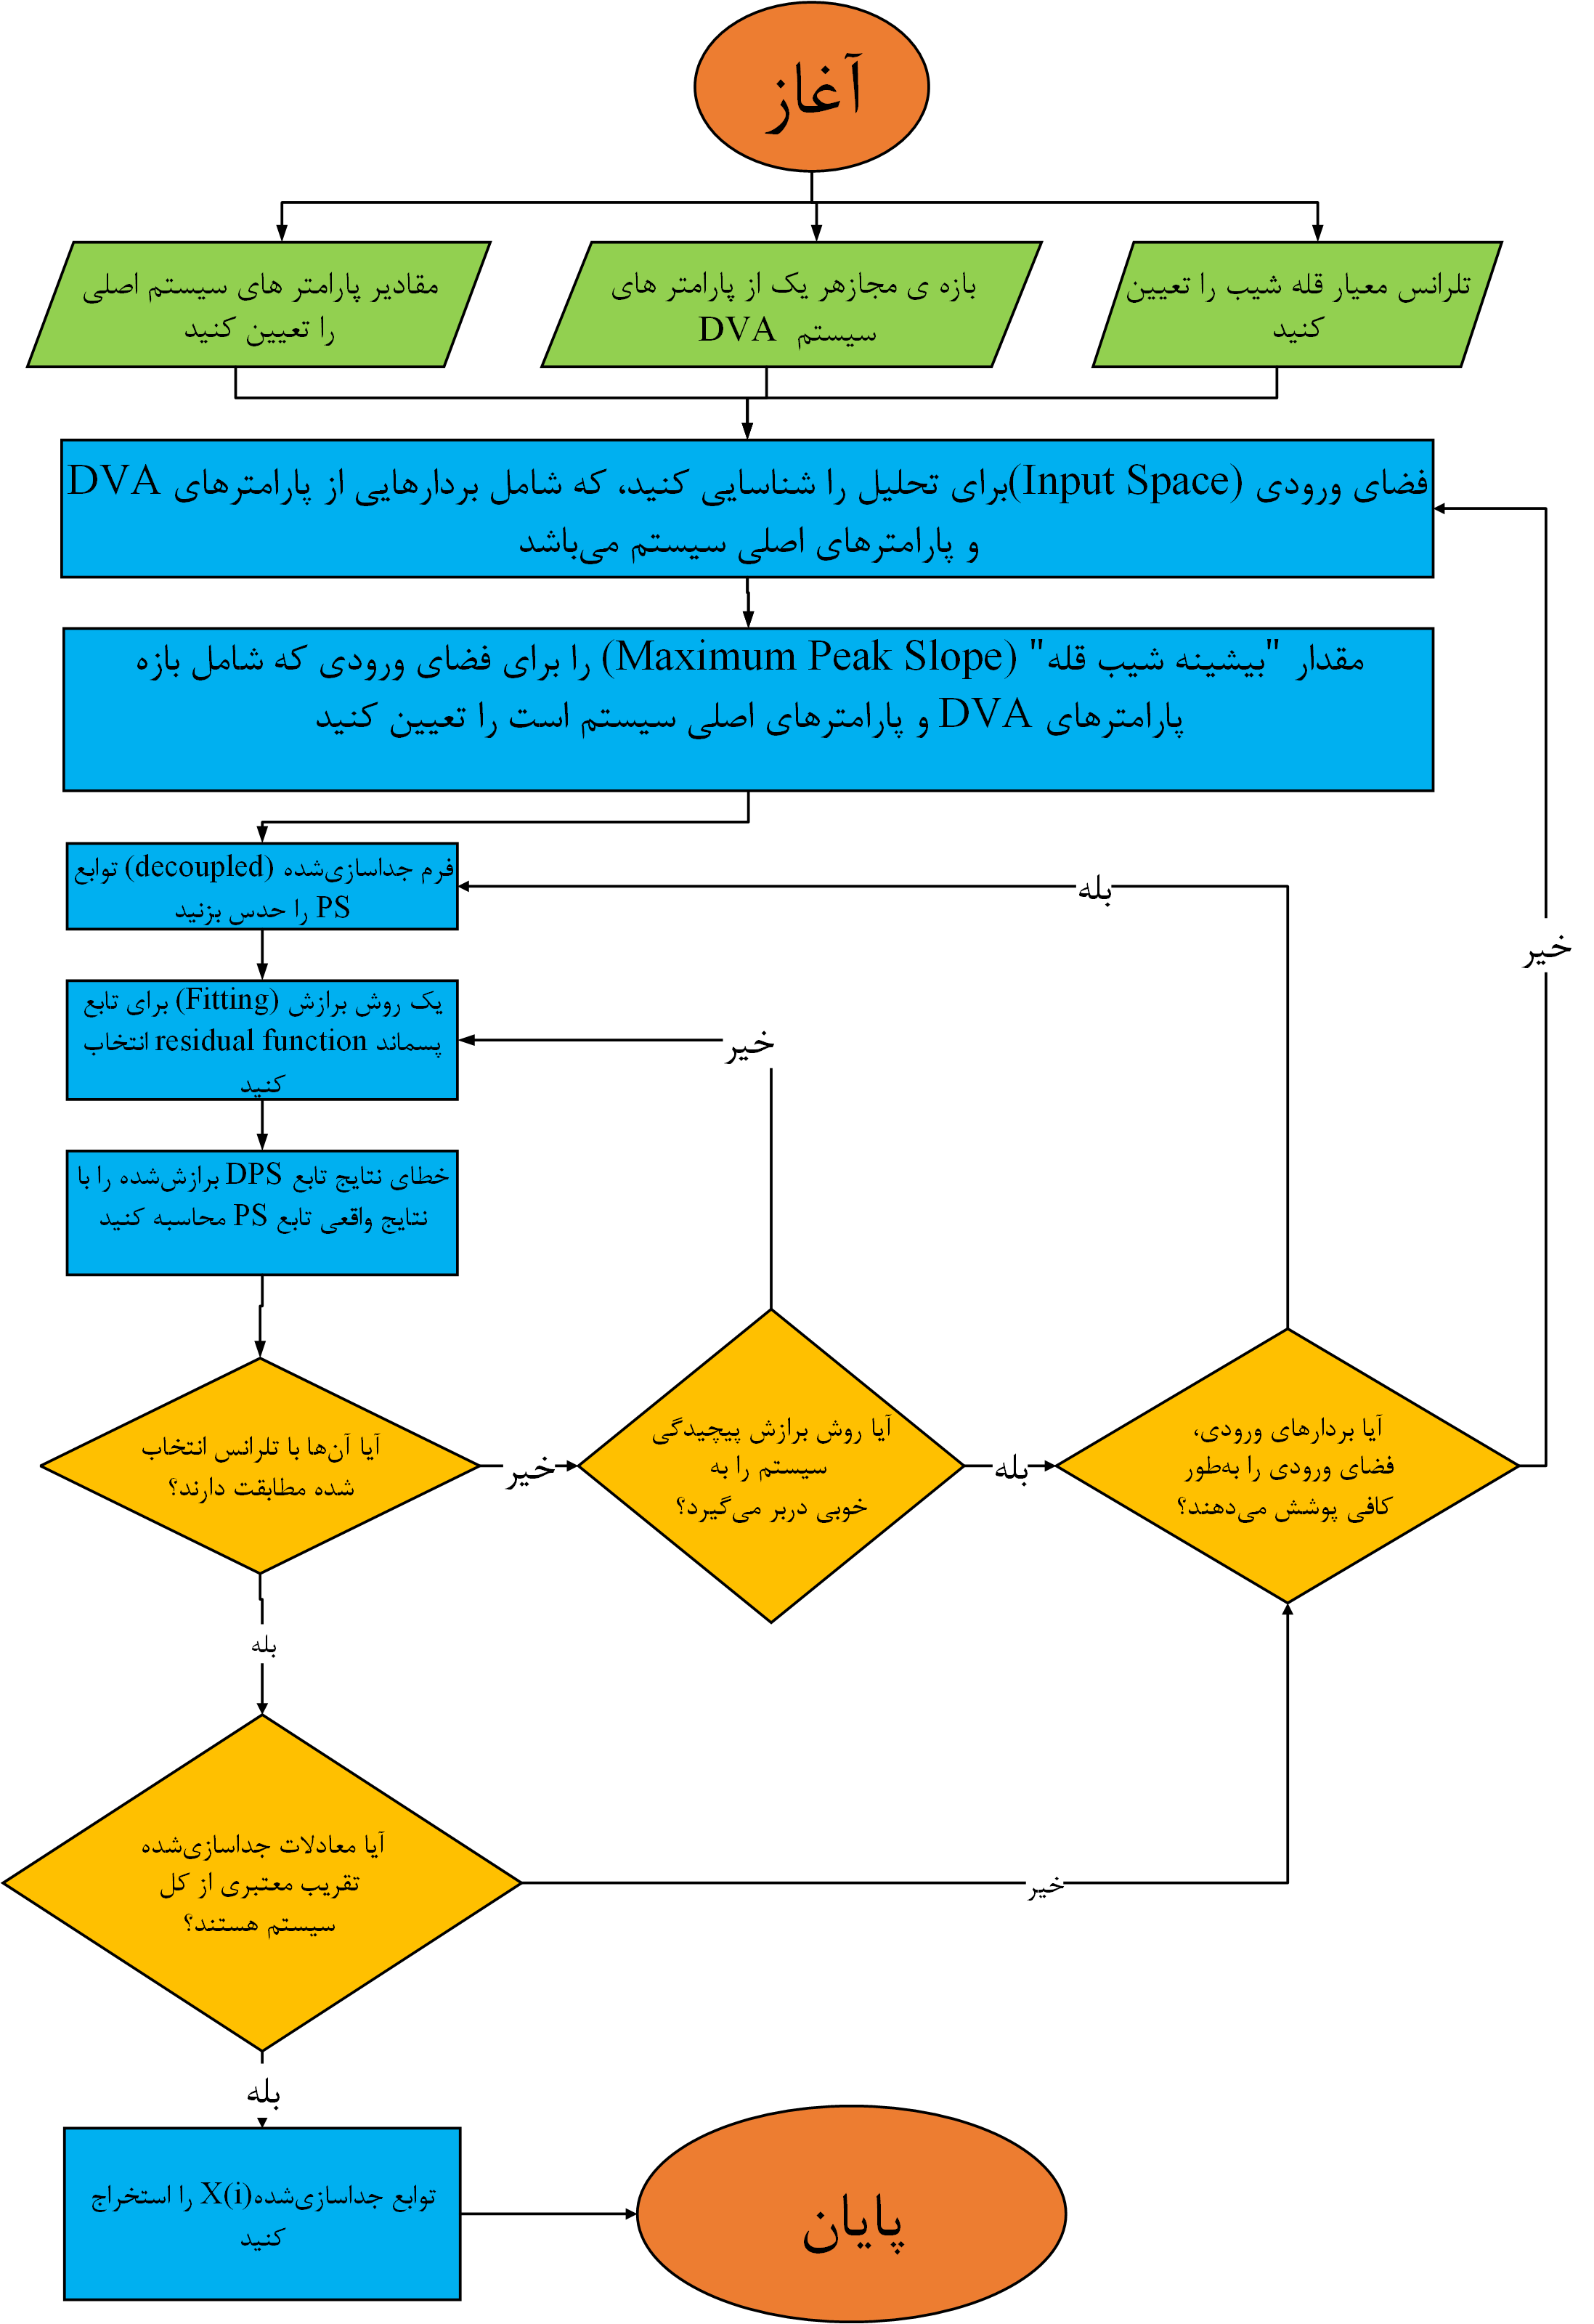
\includegraphics[width=\textwidth]{picture1.png}
        \caption{فلوچارت الگوریتم استخراج توابع جداسازی‌شده $\mathrm{DPS}^{(k)}$ از سیستم دینامیکی کاملاً کوپل شده.}
        \label{fig:dps-subfig1}
    \end{subfigure}
\end{figure}
\begin{figure}[H]
    \centering
    \begin{subfigure}[b]{\textwidth}
        \centering
        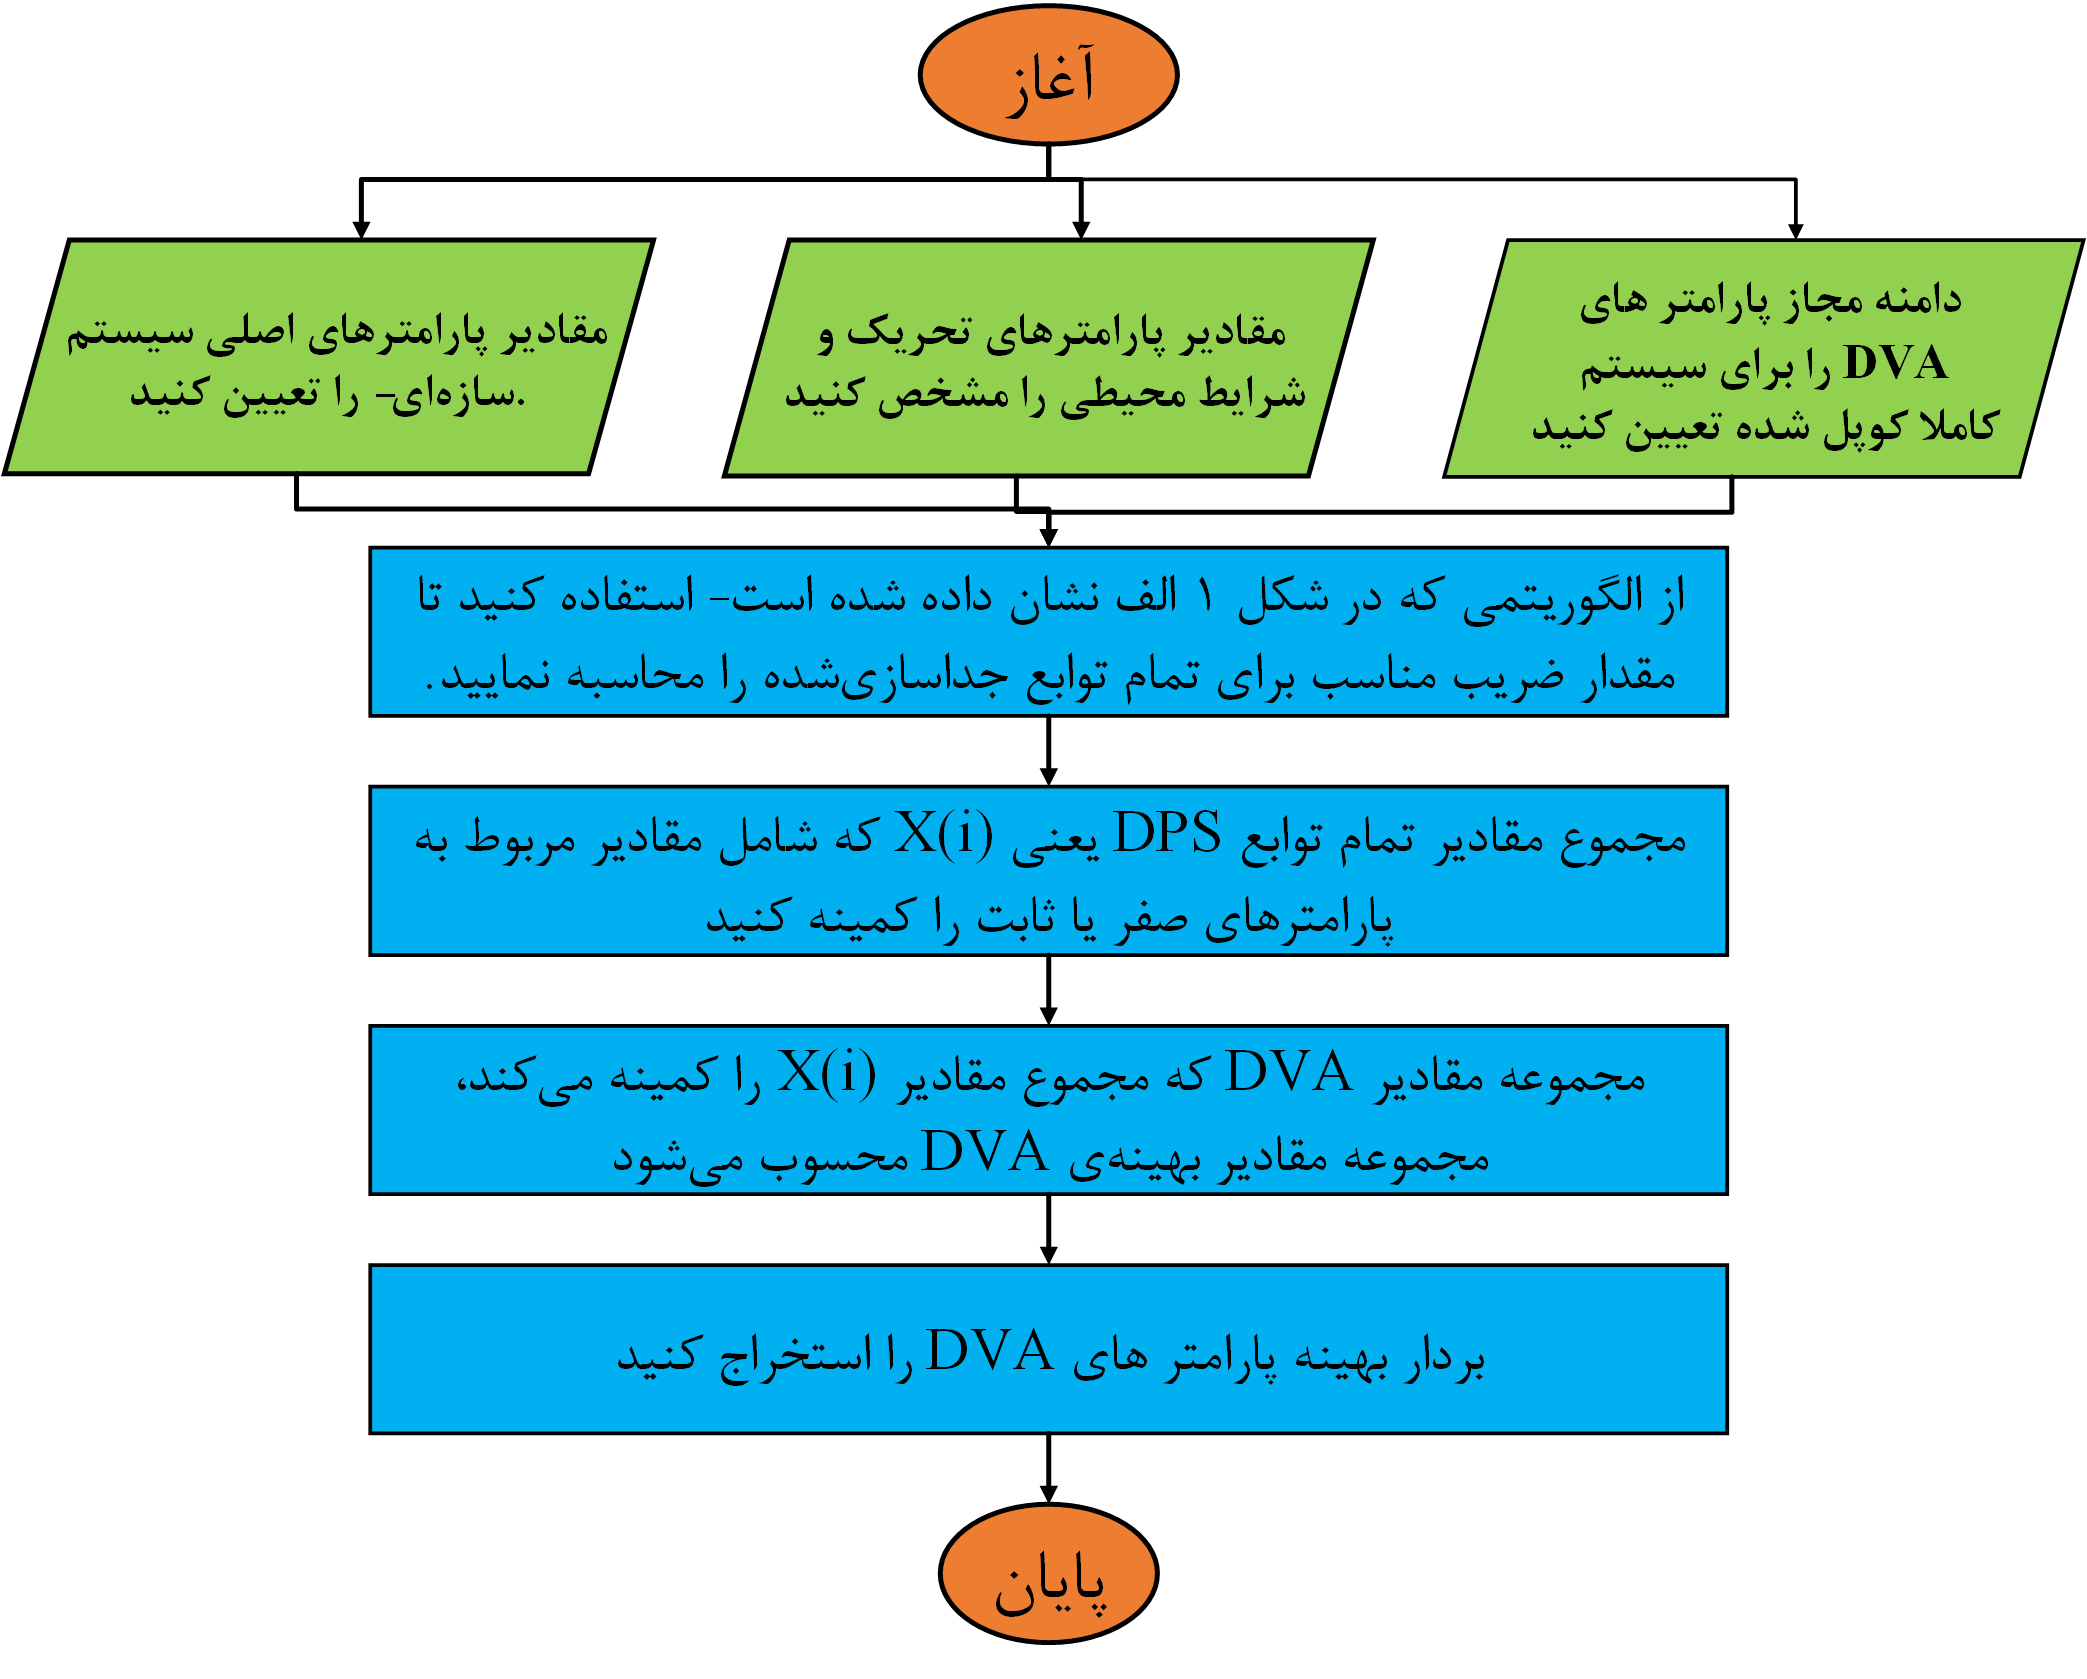
\includegraphics[width=\textwidth]{picture2.png}
        \caption{روند تعیین پارامترهای بهینه \lr{DVA} با استفاده از توابع جانشین جداسازی‌شده.}
        \label{fig:dps-subfig2}
    \end{subfigure}
    \caption{نمای کلی از الگوریتم پیشنهادی شامل (الف) استخراج توابع جداسازی‌شده \lr{DPS} از مدل کامللا کوپل شده و (ب) بهینه‌سازی پارامترهای جاذب بر پایه این توابع. هر زیرشکل در صورت نیاز به‌صورت مجزا در یک صفحه نمایش داده می‌شود.}
    \label{fig:DPS-algorithm}
\end{figure}
% --- پایان بخش --
\section{تحلیل عددی و اعتبارسنجی}

\subsection{سیستم مرجع و پارامترهای پایه}

\subsubsection{پارامترهای سیستم مرجع}

به‌منظور ارزیابی چارچوب پیشنهادی، یک تحلیل عددی با استفاده از پارامترهایی دلخواه برای سیستم اصلی انجام شده است. این پارامترها در جدول \ref{tab:main-system-parameters} ارائه شده‌اند.

\begin{table}[H]
\centering
\caption{ مقادیر عددی سیستم مورد مطالعه}
\label{tab:main-system-parameters}
\begin{tabular}{cc}
\hline
سیستم اصلی & مقدار \\
\hline
$\Lambda$ & $1$ \\
$N$ & $1$ \\
$A_{Up} = A_{Low}$ & $0.0001$ \\
$F$ & $100$ \\
$\omega_{dc}$ & $1000$ \\
$\zeta_{dc}$ & $0.01$ \\
\hline
\end{tabular}
\end{table}

مقادیر فوق به‌عنوان پایه‌ای برای آزمون عملکرد الگوریتم \lr{DPS} در شرایط کنترل‌شده استفاده شده‌اند. در ادامه، تحلیل‌های عددی و نتایج حاصل از اعمال روش پیشنهادی بر این سیستم بررسی خواهند شد.

% --- پایان بخش ---

\subsubsection{تابع جداسازی‌شده شیب-قله}

رفتار دینامیکی سیستم در چارچوب پیشنهادی با استفاده از تابع \lr{DPS} مدل‌سازی می‌شود؛ تابعی که نقش مرکزی در بهینه‌سازی دارد و به‌صورت مجموعی از ده زیرتابع مستقل تعریف می‌گردد. هر زیرتابع نمایانگر سهم یک پارامتر مشخص از سیستم در معیار کلی \lr{Peak-Slope} است:

\begin{equation}
\mathrm{DPS} = \sum_{i=1}^{10} X_i(p_i)
\end{equation}

در این رابطه، هر $X_i(p_i)$ تابعی از پارامتر خاص $p_i$ بوده و پارامترهایی نظیر $\mu$، $\beta_1$، $\lambda_1$، $\nu_1$، $\beta_2$، $\lambda_2$، $\nu_2$، $\beta_3$، $\lambda_3$ و $\nu_3$ را پوشش می‌دهد. پارامترهای اصلی سیستم (ساختار و تحریک)، به‌عنوان بخش‌های ثابت مدل واقعی، از تحلیل خارج شده‌اند تا تمرکز صرفاً بر متغیرهای قابل تنظیم جاذب باشد.

\subsubsection{شرایط اولیه}

برای شروع فرآیند تکرار، مقدار اولیه هر زیرتابع به‌صورت یکسان تعیین می‌شود:

\begin{equation}
X_i^{(0)} = X_{i,0},\quad \forall i = 1,\ldots,10
\end{equation}

که در آن $X_{i,0}$ مقدار اولیه زیرتابع $X_i$ در گام $k=0$ است.

\subsubsection{محدوده تعریف پارامترها}

هر پارامتر $p_j$ در بازه مشخصی تعریف می‌شود که به‌صورت گسسته و با گام ثابت نمونه‌برداری می‌شود:

\begin{equation}
p_j \in \left\{p_{j,i},\ p_{j,i}+\Delta p_j,\ \ldots,\ p_{j,f}\right\},\quad \forall j = 1,\ldots,10
\end{equation}

در این رابطه، $p_{j,i}$ و $p_{j,f}$ به‌ترتیب مقادیر ابتدایی و انتهایی پارامتر $p_j$ هستند و $\Delta p_j$ اندازه گام تغییرات آن است.

\subsubsection{روند تکراری به‌روزرسانی زیرتوابع}

به‌منظور محاسبه مقدار هر زیرتابع در گام بعدی، از مقدار \lr{DPS} و مجموع سایر زیرتوابع در گام قبلی استفاده می‌شود. رابطه به‌روزرسانی به‌صورت زیر تعریف می‌شود:

\begin{equation}
X_i^{(k+1)}(p_i) = \mathrm{DPS}(p_i,\text{سایر پارامترها}) - \sum_{\substack{j=1 \\ j \ne i}}^{10} X_j^{(k)}(\text{سایر پارامترها})
\end{equation}

با شرایط:
\[
\left\{
\begin{aligned}
& p_i \in \left\{p_{i,i},\ p_{i,i}+\Delta p_i,\ \ldots,\ p_{i,f} \right\} \\
& i = 1,2,\ldots,10 \\
& k = 0,1,2,\ldots
\end{aligned}
\right.
\]

در این ساختار، به‌ازای هر پارامتر متغیر، مقدار تابع مربوطه با تفریق مجموع سایر زیرتوابع از مقدار کلی \lr{DPS} محاسبه می‌شود. این فرآیند به‌صورت تکراری انجام شده و تا رسیدن به همگرایی ادامه می‌یابد.


\subsubsection{مدل‌سازی جانشین زیرتوابع}

در هر گام، مقدار محاسبه‌شده $X_i^{(k)}(p_i)$ به‌عنوان نقطه داده برای ساخت مدل جانشین مربوط به پارامتر $p_i$ در نظر گرفته می‌شود. برای تقریب رفتار این توابع در طول تکرار، از مدل‌های چندجمله‌ای (مانند رگرسیون چهارم‌درجه) استفاده می‌شود که تعادل مناسبی بین دقت و سرعت محاسباتی فراهم می‌آورند.

این مدل‌های جانشین، پایه اصلی بهینه‌سازی تابع \lr{DPS} را تشکیل می‌دهند و امکان تحلیل سریع، کاهش نیاز به شبیه‌سازی‌های پیچیده، و استخراج پارامترهای بهینه با دقت بالا را فراهم می‌سازند.

% --- پایان بخش ---

\subsubsection{ارزیابی کارایی مدل‌های تقریب‌زا}

برای تعیین دقیق‌ترین روش تقریب تابع جزئی \lr{DPS}، عملکرد چندین مدل برازش چندجمله‌ای ارزیابی شد. نتایج این تحلیل در شکل \ref{fig:polyfit-comparison} و جدول \ref{tab:polyfit-error} ارائه شده‌اند. ارزیابی‌ها بر پایه خطای میانگین، انحراف معیار و ریشه میانگین مربعات خطا (\lr{RMSE}) صورت گرفت. در هر زیرنمودار از شکل \ref{fig:polyfit-comparison}، محور افقی بیانگر مقادیر واقعی \lr{PS} و محور عمودی بیانگر مقادیر پیش‌بینی‌شده توسط مدل است. هر نقطه نشان‌دهنده یک مجموعه پارامتر منحصر به‌فرد برای \lr{DVA} است. خط‌چین قرمز، خط برازش کامل یا ایده‌آل را نمایش می‌دهد.

با افزایش درجه چندجمله‌ای، دقت تقریب به‌طور قابل‌ملاحظه‌ای افزایش یافت. برازش خطی (شکل \ref{fig:polyfit-comparison}–الف) بیشترین خطا را نشان داد و مقدار \lr{RMSE} برابر با $1.4430\times10^{-10}$ بود. برازش درجه دوم (شکل \ref{fig:polyfit-comparison}–ب) خطا را به $8.3068\times10^{-11}$ کاهش داد. در ادامه، مدل مکعبی (شکل \ref{fig:polyfit-comparison} ج) عملکرد بهتری ارائه داد ($\mathrm{RMSE}=1.9874\times10^{-11}$). در نهایت، برازش درجه چهارم (شکل \ref{fig:polyfit-comparison} د) کمترین میزان خطا را با $\mathrm{RMSE}=2.9908\times10^{-12}$ به‌دست آورد و بیشترین هم‌خوانی با خط برازش کامل را از خود نشان داد.

بنابراین، براساس نتایج کمی و کیفی، چندجمله‌ای مرتبه چهارم به‌عنوان دقیق‌ترین و بهینه‌ترین روش برای تقریب تابع \lr{DPS} انتخاب شد.

\begin{figure}
    \centering
    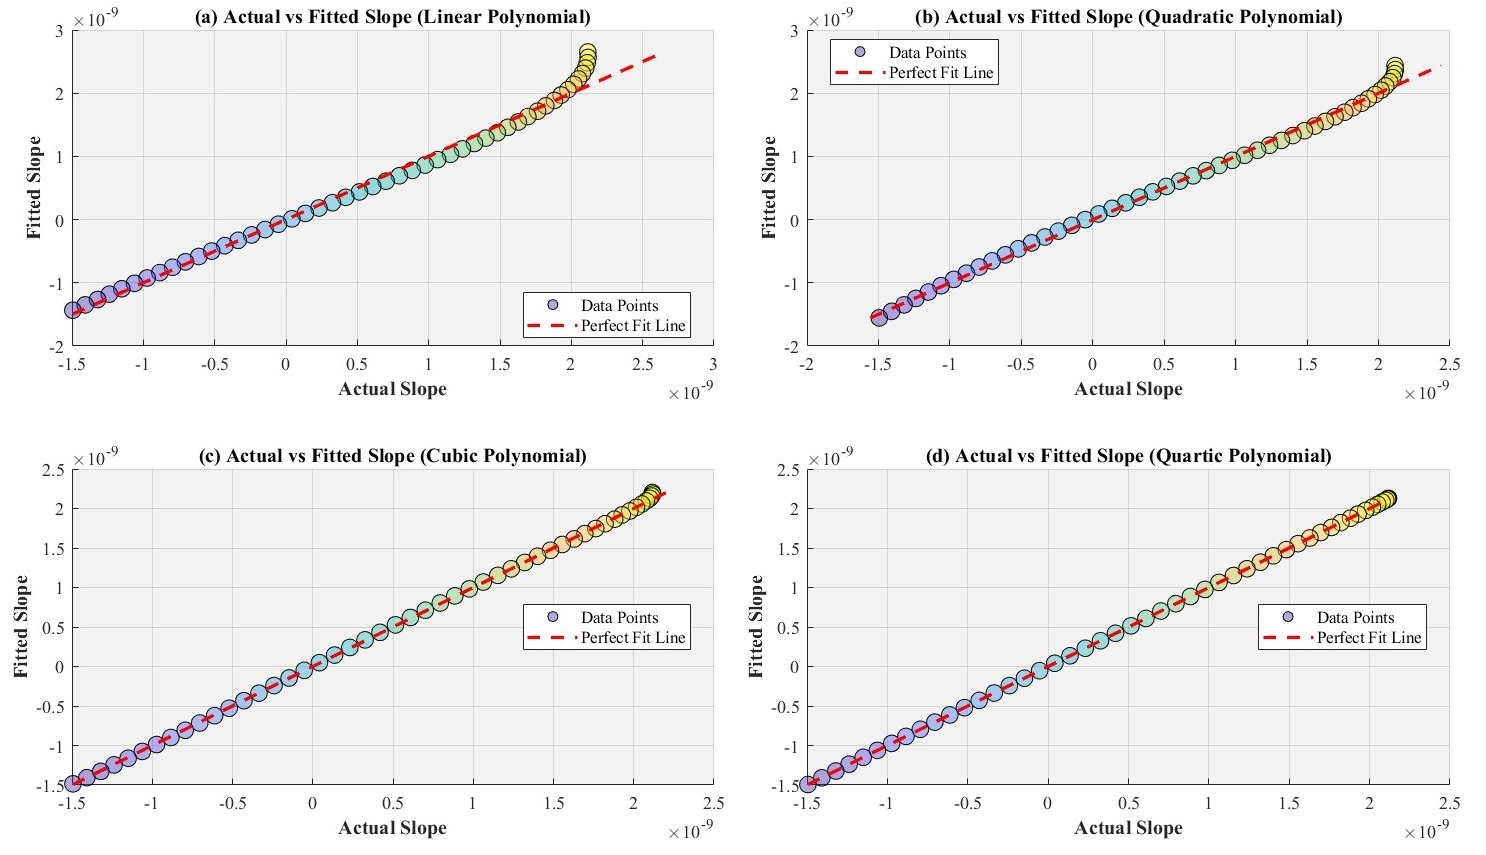
\includegraphics[width=1.1\textwidth]{picture4.png}
    \caption{مقایسه روش‌های برازش چندجمله‌ای برای تابع \lr{DPS}: (الف) خطی، (ب) درجه دوم، (ج) درجه سوم، (د) درجه چهارم. خط‌چین قرمز: برازش ایده‌آل، نقاط: مقادیر واقعی در برابر مقادیر پیش‌بینی‌شده}
    \label{fig:polyfit-comparison}
\end{figure}


\begin{table}[h]
    \centering
    \caption{مقایسه آماری خطای برازش مدل‌های چندجمله‌ای}
    \label{tab:polyfit-error}
    \begin{tabular}{cccc}
        \hline
        \lr{Fitting Method} & \lr{Mean Error} & \lr{STD} & \lr{RMSE} \\
        \hline
        \lr{Linear Polynomial}   & $9.6730\times10^{-11}$ & $1.0819\times10^{-10}$ & $1.4430\times10^{-10}$ \\
        \lr{Quadratic Polynomial} & $5.8807\times10^{-11}$ & $5.9277\times10^{-11}$ & $8.3068\times10^{-11}$ \\
        \lr{Cubic Polynomial}     & $1.2789\times10^{-11}$ & $1.5370\times10^{-11}$ & $1.9874\times10^{-11}$ \\
        \lr{Quartic Polynomial}   & $1.5188\times10^{-12}$ & $2.6031\times10^{-12}$ & $2.9908\times10^{-12}$ \\
        \hline
    \end{tabular}
\end{table}
% --- پایان بخش ---
\subsection{مقایسه با روش‌های مرجع و ارزیابی عملکرد}

\subsubsection{مقایسه با الگوریتم ژنتیک}

برای ارزیابی عملکرد چارچوب پیشنهادی \lr{DPS}، یک الگوریتم ژنتیک (\lr{Genetic Algorithm} یا \lr{GA}) با شرایط طراحی یکسان پیکربندی شد تا به‌عنوان مبنای مقایسه عمل کند. پارامترهای الگوریتم \lr{GA} شامل اندازه جمعیت برابر با ۱۵۰، تعداد نسل‌ها ۲۰، احتمال تلاقی ۰.۷۰ و احتمال جهش ۰.۲۰ در نظر گرفته شدند. تمام پارامترهای جاذب ارتعاش در بازه $[0, 1]$ مقید شدند، به‌جز نسبت جرم $\mu^1$ که در بازه $[0, 0.75]$ محدود شد. هر ارزیابی توسط الگوریتم \lr{GA} نیازمند محاسبه کامل پاسخ فرکانسی سیستم بود، در حالی که روش \lr{DPS} از ارزیابی‌های تحلیلی مبتنی بر مدل جانشین استفاده می‌کند.

برای بررسی رفتار تصادفی \lr{GA}، صد اجرای مستقل با بذرهای تصادفی متفاوت انجام شد. اگرچه در برخی موارد الگوریتم موفق به یافتن مقدار بهینه برای \lr{PS} شد، اما نوسان زیادی در نتایج مشاهده گردید. بهترین مقدار \lr{PS} حاصل از \lr{GA} برابر با $4.3 \times 10^{-5}$، میانگین برابر با $4.4 \times 10^{-5}$ و بدترین نتیجه برابر با $1.4 \times 10^{-4}$ بود. در مقابل، روش \lr{DPS} به‌صورت قطعی و در تنها یک بار اجرا، مقدار $6.9344 \times 10^{-5}$ را برای \lr{PS} به‌دست آورد.

در جدول \ref{tab:DPS-vs-GA} مقایسه‌ای بین مقادیر پارامترهای بهینه حاصل از روش \lr{DPS} و مقادیر حاصل از بهترین، میانگین و بدترین اجرای الگوریتم ژنتیک ارائه شده است. با وجود آنکه مقدار \lr{PS} به‌دست‌آمده از \lr{DPS} کمی بیشتر از بهترین نتیجه \lr{GA} است، اما این نتیجه با سرعت بالا، بدون تصادف، و تنها در یک مرحله محاسبه حاصل شده است.

\begin{table}[H]
\centering
\caption{مقایسه پارامترهای بهینه و مقادیر \lr{PS} بین روش \lr{DPS} و الگوریتم ژنتیک}
\label{tab:DPS-vs-GA}
\begin{latin}
\begin{tabular}{lcccc}
\hline
\textbf{Parameter} & \textbf{DPS Optimum} & \textbf{Best GA} & \textbf{Mean GA} & \textbf{Worst GA} \\
\hline
PS & $6.9344 \times 10^{-5}$ & $4.3 \times 10^{-5}$ & $4.4 \times 10^{-5}$ & $1.4 \times 10^{-4}$ \\
\hline
$\beta^1$ & 0.79 & 0.006 & 0.104 & 0.63 \\
$\beta^2$ & 0.98 & 0.467 & 0.047 & 0.71 \\
$\beta^3$ & 0.47 & 0.338 & 0.422 & 0.31 \\
$\lambda^1$ & 1.99 & 0.96 & 0.89 & 0.23 \\
$\lambda^2$ & 0.83 & 0.62 & 0.57 & 0.72 \\
$\lambda^3$ & 1.68 & 0.57 & 0.43 & 1.00 \\
$\mu^1$ & 0.17 & 0.49 & 0.05 & 0.40 \\
$\nu^1$ & 1.69 & 0.78 & 0.18 & 1.00 \\
$\nu^2$ & 1.49 & 0.13 & 0.54 & 0.97 \\
$\nu^3$ & 2.35 & 0.32 & 0.18 & 0.57 \\
\hline
\end{tabular}
\end{latin}
\end{table}

نمودار شکل \ref{fig:frf-dps-vs-ga} مقایسه‌ای بصری از توابع پاسخ فرکانسی (\lr{FRF}) به‌دست‌آمده از روش \lr{DPS} و سه نمونه‌نماینده از بین صد اجرای \lr{GA} را نمایش می‌دهد: بهترین، میانگین و بدترین حالت. در نتایج مربوط به حالت‌های بهترین و میانگین \lr{GA}، قله‌های پاسخ با تعادل مناسبی تنظیم شده‌اند و مقادیر \lr{PS} به‌دست‌آمده کمی کمتر از مقدار حاصل از \lr{DPS} هستند که نشان‌دهنده موفقیت در تنظیم جاذب می‌باشد. با این حال، نتیجه مربوط به بدترین حالت \lr{GA} عدم تعادل واضحی در قله‌ها نشان می‌دهد، که بیانگر ضعف این روش در تولید پاسخ‌های پایدار است.

این مقایسه به‌خوبی یکی از محدودیت‌های ذاتی روش‌های مبتنی بر \lr{GA} را آشکار می‌سازد: ذات احتمالی این الگوریتم‌ها منجر به تغییرپذیری در کیفیت نتایج می‌شود و برای دستیابی به پاسخ مناسب، نیاز به تکرارهای متعدد دارند. در مقابل، روش \lr{DPS} به‌صورت قطعی، تنها با یک‌بار اجرا و بدون تصادف، پاسخی با کیفیت بالا تولید می‌کند. اگرچه تنظیم قله‌ها در روش \lr{DPS} همیشه بهتر از بهترین اجرای \lr{GA} نیست، اما پایداری، سرعت بالا، و هزینه محاسباتی ناچیز، آن را به گزینه‌ای برتر برای کاربردهای زمان‌حقیقی یا طراحی سریع تبدیل می‌کند.

\begin{figure}[H]
    \centering
    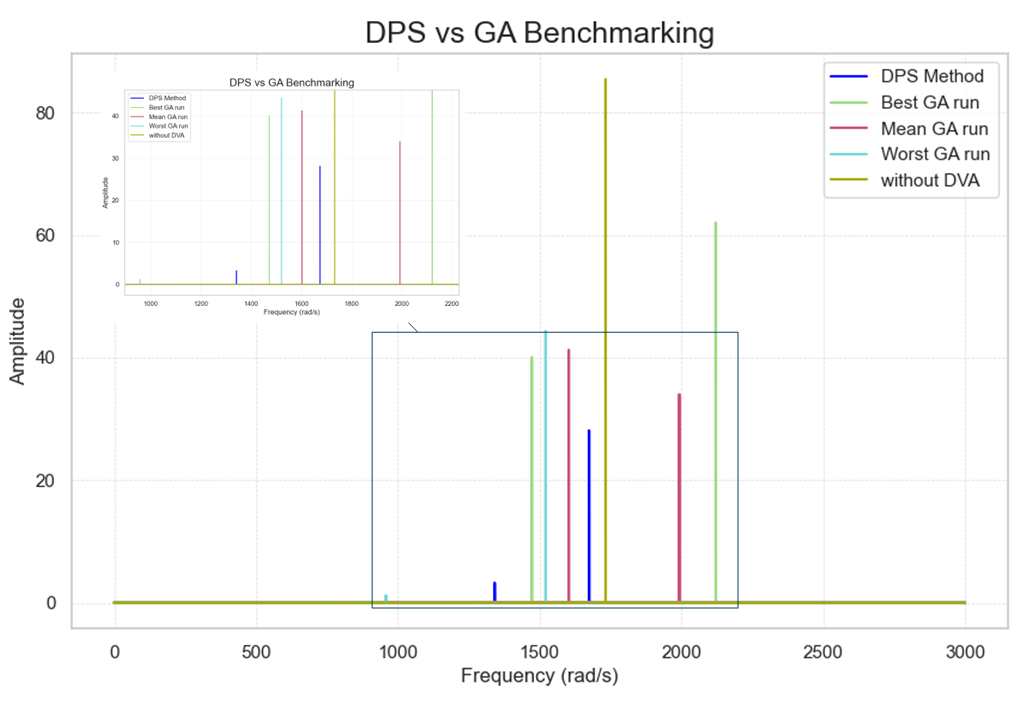
\includegraphics[width=0.85\textwidth]{picture5.png}
    \caption{مقایسه \lr{FRF} بین روش \lr{DPS} و نمونه‌های برتر، میانگین و ضعیف الگوریتم ژنتیک برای سیستم مرجع}
    \label{fig:frf-dps-vs-ga}
\end{figure}

این بررسی نه‌تنها اثربخشی عددی روش پیشنهادی را تأیید می‌کند، بلکه از طریق شواهد بصری و مقایسه‌ای، درک عمیق‌تری از عملکرد آن فراهم می‌آورد؛ به‌ویژه برای خوانندگانی که به دنبال تحلیل‌های کاربردی و قابل تکرار هستند.

% --- پایان بخش ---


\subsubsection{اعتبارسنجی با مدل‌های تحلیلی مرتبه پایین}

برای ارزیابی دقت و پایداری روش پیشنهادی \lr{DPS}، یک مطالعه اعتبارسنجی با استفاده از سیستمی با درجه آزادی پایین و دارای راه‌حل تحلیلی شناخته‌شده انجام شد. منطق اصلی این ارزیابی بر پایه این فرض استوار است که اگر فرایند جداسازی پارامترها در چارچوب \lr{DPS} به‌درستی انجام شده باشد، آنگاه معادلات مدل جانشین مشتق‌شده از یک سیستم کاملاً کوپله باید قادر باشند پاسخ‌های صحیحی حتی در مدل‌های ساده‌تر نیز ارائه دهند. چنین نتیجه‌ای نشان‌دهنده جداسازی کامل دینامیک کوپله اولیه خواهد بود.

برای این منظور، از سیستم \lr{1DOF–1DOF} کاملاً کوپله معرفی‌شده در فصل‌های قبل به‌عنوان مبنای ساخت مدل جانشین استفاده شد، اما در مرحله اعتبارسنجی، چارچوب \lr{DPS} بر روی سیستم ساده‌شده‌ای که توسط \lr{Asami et al.} \cite{asami2002analytical} ارائه شده اعمال گردید. در این پیکربندی، جرم اصلی به یک پایه صلب از طریق یک فنر و میرای متصل است و جرم جاذب نیز به جرم اصلی از طریق یک جفت فنر–میرای دیگر متصل می‌گردد (شکل \ref{fig:asami-validation-diagram}).

\begin{figure}[h]
\centering
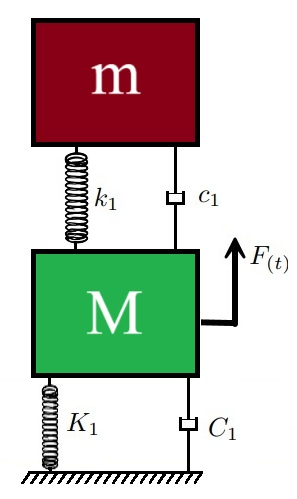
\includegraphics[width=0.25\textwidth]{picture6.png}
\caption{شماتیک سیستم مورد استفاده برای اعتبارسنجی، برگرفته از \lr{Asami et al.} \cite{asami2002analytical}}
\label{fig:asami-validation-diagram}
\end{figure}

در مطالعه‌ی \lr{Asami et al.}، پاسخ‌های تحلیلی مرتبه اول و دوم برای این سیستم استخراج شده‌اند. این پاسخ‌ها به‌عنوان معیارهای مرجع برای مقایسه با نتایج روش \lr{DPS} مورد استفاده قرار گرفتند. در این آزمایش، پارامترهای ساختاری به صورت ثابت در نظر گرفته شدند: فرکانس طبیعی $\Omega_{dc} = 14.14 \Omega$، نسبت میرایی $\zeta_{dc} = 0.24$، نیروی تحریک برابر با ۱۰۰ نیوتن و نسبت جرم $\mu = 0.5$. هدف بهینه‌سازی، تعیین نسبت سختی $\lambda_1$ و نسبت میرایی $\nu_1$ جاذب بود به‌گونه‌ای که معیار \lr{PS} به حداقل برسد. نتایج بهینه‌سازی برای هر سه روش در جدول \ref{tab:asami-comparison} ارائه شده است.

\begin{table}[h]
\centering
\caption{مقایسه پارامترهای بهینه و مقدار \lr{PS} برای سیستم مرجع \lr{Asami et al.} \cite{asami2002optimum}}
\label{tab:asami-comparison}
\begin{tabular}{lccc}
\hline
روش & $\boldsymbol{\lambda}_\mathbf{1}$ & $\boldsymbol{\nu}_\mathbf{1}$ & مقدار \lr{PS} \\
\hline
تحلیلی مرتبه اول (\lr{Asami}) & \lr{0.1525} & \lr{4.568} & \lr{0.59913} \\
تحلیلی مرتبه دوم (\lr{Asami}) & \lr{0.1250} & \lr{4.041} & \lr{0.38587} \\
روش \lr{DPS} پیشنهادی & \lr{0.1280} & \lr{3.381} & \lr{0.04915} \\
\hline
\end{tabular}
\end{table}


شکل \ref{fig:asami-frf-comparison}(الف) تابع پاسخ فرکانسی (\lr{FRF}) حاصل از سه روش را نمایش می‌دهد. همان‌طور که مشاهده می‌شود، هر سه روش پاسخ کلی مشابهی ارائه می‌دهند که صحت چارچوب \lr{DPS} را به‌طور کلی تأیید می‌کند. با این حال، بررسی دقیق‌تر در شکل \ref{fig:asami-frf-comparison}(ب) نشان داده شده که در آن مقادیر معیار \lr{PS} به‌صورت نمودار میله‌ای مقایسه شده‌اند. در این نمودار، مقدار \lr{PS} حاصل از روش \lr{DPS} نزدیک به یک مرتبه کوچکتر از دو روش تحلیلی است که این امر نشان‌دهنده تعادل بهتر بین قله‌ها و تنظیم دقیق‌تر جاذب می‌باشد.

\begin{figure}[h]
\centering
\subfloat[\lr{FRF} حاصل از سه روش مختلف]{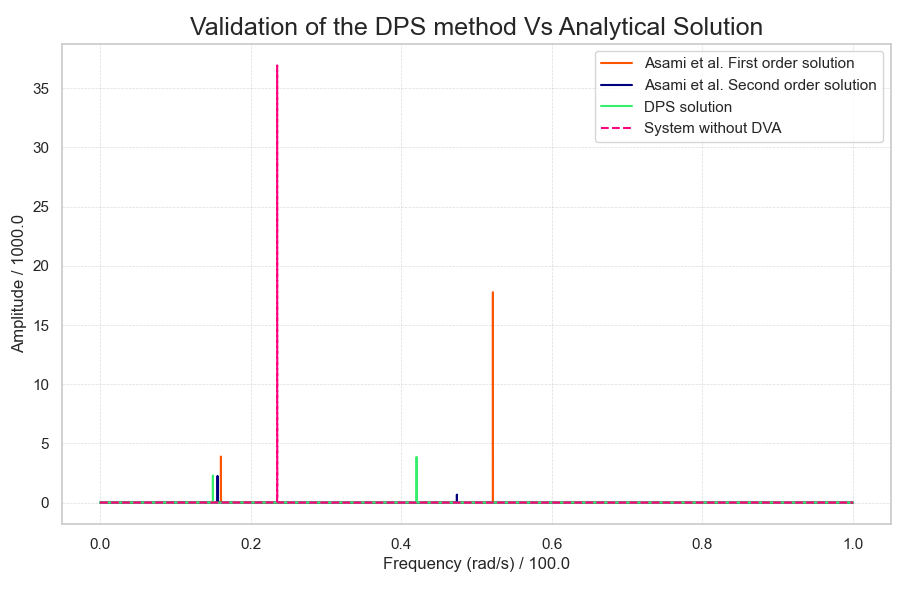
\includegraphics[width=0.5\textwidth]{picture8.png}}
\hfill
\subfloat[مقایسه مقادیر معیار \lr{PS}]{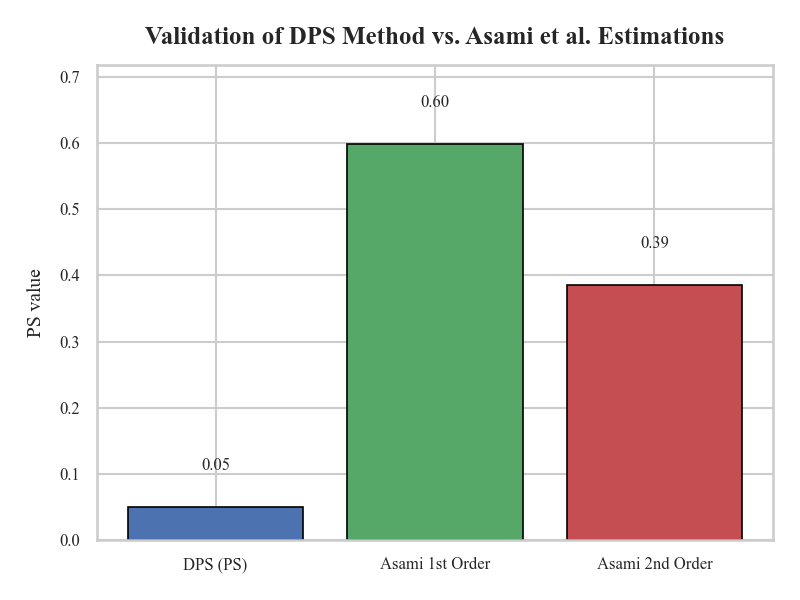
\includegraphics[width=0.5\textwidth]{picture7.png}}
\caption{مقایسه پاسخ‌های فرکانسی و معیار \lr{PS} بین روش \lr{DPS} و پاسخ‌های تحلیلی \lr{Asami}}
\label{fig:asami-frf-comparison}
\end{figure}

این نتایج تأیید می‌کنند که فرض جداسازی پارامترها در روش \lr{DPS} حتی در سیستم‌های ساده با درجات آزادی پایین نیز معتبر است. به‌عبارت دیگر، اگر روش در چنین شرایطی عملکرد دقیق داشته باشد، می‌توان انتظار داشت در سیستم‌های پیچیده‌تر با درجات آزادی بالا نیز به‌خوبی عمل کند. نکته کلیدی این است که فرآیند بهینه‌سازی در \lr{DPS} تنها بر اساس کمینه‌سازی جمع توابع جانشین از پیش محاسبه‌شده انجام می‌گیرد، بدون نیاز به شبیه‌سازی‌های تکراری سیستم کامل. این ویژگی فرآیند سنتی و پرهزینه تنظیم جاذب‌ها را به یک فرایند ساختارمند، تکرارپذیر و کم‌هزینه تبدیل می‌کند.

در نهایت، با امکان استفاده مستقیم از این توابع جانشین در معماری‌های مختلف سیستم، چارچوب \lr{DPS} بستری برای توسعه کاتالوگ‌های طراحی فراهم می‌آورد که نیاز به بهینه‌سازی‌های عددی مجدد را حذف کرده و انتخاب سریع پارامترهای نزدیک به بهینه را برای مهندسان ممکن می‌سازد.

% --- پایان بخش ---
% -----------------------------
% Section: Generalized Optimization with DPS-Derived Catalogues
% -----------------------------

\section{کاتالوگ‌های طراحی تعمیم‌یافته}

\subsection{الگوریتم کاتالوگ‌سازی و کاربردهای تعمیم‌یافته}

پس از اعتبارسنجی موفق چارچوب \lr{DPS}، در این بخش الگوریتمی ساختاریافته برای تولید کاتالوگ‌های طراحی معرفی می‌شود که امکان بهینه‌سازی سریع پارامترهای جاذب دینامیکی ارتعاش را برای مجموعه‌ای گسترده از سیستم‌های مکانیکی فراهم می‌سازد. این قابلیت حتی برای سیستم‌هایی که تنها زیرمجموعه‌ای ساده‌شده از مدل مرجع کوپله‌شده کامل هستند نیز کاربرد دارد. اصل بنیادی چارچوب \lr{DPS} در جداسازی فضای بهینه‌سازی نهفته است؛ بدین‌گونه که هر پارامتر جاذب به تابع جانشین تک‌متغیره مستقل خود وابسته است که از مدل دینامیکیِ کامل استخراج شده است.

این رویکرد به‌گونه‌ای طراحی شده است که معادلات جداسازی‌شده حاصل، قابلیت اعمال عمومی داشته باشند و در هر پیکربندی سیستمی که درون دامنه‌های پارامترِیِ مدل‌سازی‌شده قرار گیرد، قابل استفاده باشند؛ حتی در صورتی که بعضی اجزای سیستم کامل در پیکربندی موردنظر وجود نداشته باشند. منطقِ الگوریتم جداسازی این امکان را فراهم می‌کند که چنانچه یک سامانه فاقد برخی مؤلفه‌ها باشد (برای مثال، بدون المان \lr{Inerter} یا با مقدار میراییِ قفل‌شده)، پارامتر مربوطه یا مقدار صفر در نظر گرفته شود (در صورت نبود) و یا به‌عنوان مقدار ثابت جای‌گذاری شود (در صورت قفل بودن). با این‌حال، حتی اگر مقدار یک پارامتر صفر باشد، تابع جانشین مربوطه باید همچنان در فرآیند بهینه‌سازی ارزیابی شود تا اثرات پسماند ناشی از مدل کامل در پیکربندی کاهش‌یافته نیز لحاظ گردد.

هدف بهینه‌سازی در این الگوریتم به‌صورت کمینه‌سازی مجموع تمام توابع جانشینِ جداسازی‌شده تعریف می‌شود، صرف‌نظر از این‌که پارامتر متناظر در سیستم حضور داشته باشد یا خیر. در این فرمول‌بندی، مجموعه بهینه پارامترهای جاذب زمانی حاصل می‌شود که مجموع این توابع به حداقل برسد؛ بدین معنا که نوسان بین قله‌های پاسخ به کمترین میزان رسیده و جذب ارتعاش در حالت بهینه صورت گرفته است:

\begin{equation}
\min_{\{p_i\}} \; \sum_{i=1}^{n} X_i\bigl(p_i\bigr)
\end{equation}

در این‌جا \(n\) تعداد کل توابعِ جداسازی‌شده استخراج‌شده از مدل کامل است (حتی پارامترهای غیرفعال یا صفر را شامل می‌شود).

به‌منظور پشتیبانی از این رویکرد الگوریتمی، یک کاتالوگ طراحی بر اساس چهار پیکربندی ساختاریِ متفاوت از مدل مرجع توسعه داده شد. هر پیکربندی با مجموعه‌ای مشخص از ویژگی‌های ساختاریِ ثابت مانند فرکانس طبیعی، نسبت میرایی و نسبت جرم مشخص می‌شود. برای هر پیکربندی، ده تابع جانشینِ جداسازی‌شده تولید گردید که هرکدام نمایانگر تأثیر یک پارامتر خاص از جاذب ارتعاش هستند. این توابع جانشین به‌صورت چندجمله‌ایِ درجه چهارم مدل‌سازی شده‌اند:

\begin{equation}
X_i(p_i) 
  = a_{i,0} + a_{i,1} p_i + a_{i,2} p_i^{2} + a_{i,3} p_i^{3} + a_{i,4} p_i^{4}
\end{equation}

ضرایب چندجمله‌ای \(a_{i,k}\) برای هر تابع، به‌همراه ویژگی‌های ساختاریِ هر مورد، در جدول~\ref{tab:structural-params} و جداول ضرایبِ بعدی ارائه شده‌اند.

% --------------------------------------------------------
% Structural parameters of the four reference systems
% --------------------------------------------------------

\begin{table}[ht]
  \centering
  \caption{پارامترهای ساختاری چهار سیستم مرجع}
  \label{tab:structural-params}
  \begin{tabular}{c c c c c c c}
    \hline
    \lr{System} & $\Lambda$ & $N$ & $A_{Up}{=}A_{Low}$ & $F$ & $\omega_{dc}$ & $\zeta_{dc}$ \\
    \hline
    \lr{1} & \lr{1.00} & \lr{1.00} & \lr{1e-4} & \lr{100} & \lr{1000} & \lr{0.01} \\
    \lr{2} & \lr{0.75} & \lr{0.75} & \lr{1e-4} & \lr{100} & \lr{800}  & \lr{0.02} \\
    \lr{3} & \lr{0.50} & \lr{0.50} & \lr{1e-4} & \lr{100} & \lr{800}  & \lr{0.02} \\
    \lr{4} & \lr{0.50} & \lr{0.50} & \lr{1e-4} & \lr{100} & \lr{700}  & \lr{0.03} \\
    \hline
  \end{tabular}
\end{table}

\bigskip

% --------------------------------------------------------
% Polynomial coefficients tables (Systems 1--4)
% --------------------------------------------------------

% ---------- System 1 ----------
\begin{table}[ht]
  \centering
  \scriptsize
  \caption{ضرایب چندجمله‌ای چارچوب \protect\lr{DPS} برای سیستم \protect\lr{1}}
  \label{tab:dps-coeff-sys1}
  \begin{tabular}{l r r r r r}
    \hline
      & $a_{4}$ & $a_{3}$ & $a_{2}$ & $a_{1}$ & $a_{0}$ \\
    \hline
    $\mu_{1}$     & \lr{$-8.2269e-12$} & \lr{$2.2743e-10$} & \lr{$-2.1919e-09$} & \lr{$8.5432e-09$}  & \lr{$-1.1436e-08$} \\
    $\beta_{1}$   & \lr{$1.2785e-11$}  & \lr{$-2.9913e-10$} & \lr{$2.6576e-09$}  & \lr{$-8.3011e-09$} & \lr{$-2.7080e-09$} \\
    $\lambda_{1}$ & \lr{$3.3333e-12$}  & \lr{$-1.1461e-10$} & \lr{$6.9518e-10$}  & \lr{$-2.7359e-10$} & \lr{$1.1169e-09$} \\
    $\nu_{1}$     & \lr{$3.4793e-12$}  & \lr{$-7.5003e-11$} & \lr{$5.1341e-10$}  & \lr{$-2.7621e-09$} & \lr{$1.5231e-08$} \\
    $\beta_{7}$   & \lr{$4.3369e-11$}  & \lr{$-9.1300e-10$} & \lr{$5.6815e-09$}  & \lr{$-1.1223e-08$} & \lr{$2.5909e-08$} \\
    $\lambda_{7}$ & \lr{$-4.6563e-11$} & \lr{$9.9032e-10$}  & \lr{$-6.4370e-09$} & \lr{$1.3672e-08$}  & \lr{$-2.7614e-08$} \\
    $\nu_{7}$     & \lr{$-3.1186e-12$} & \lr{$8.3988e-11$}  & \lr{$-5.1866e-10$} & \lr{$9.5108e-10$}  & \lr{$-1.3858e-10$} \\
    $\beta_{8}$   & \lr{$-3.0277e-11$} & \lr{$1.1787e-09$}  & \lr{$-1.5057e-08$} & \lr{$6.9366e-08$}  & \lr{$-6.3326e-08$} \\
    $\lambda_{8}$ & \lr{$2.4785e-11$}  & \lr{$-1.0481e-09$} & \lr{$1.3963e-08$}  & \lr{$-6.5790e-08$} & \lr{$6.0165e-08$} \\
    $\nu_{8}$     & \lr{$1.7830e-13$}  & \lr{$-2.1887e-11$} & \lr{$5.8945e-10$}  & \lr{$-4.1231e-09$} & \lr{$4.9205e-09$} \\
    \hline
  \end{tabular}
\end{table}

% ---------- System 2 ----------
\begin{table}[ht]
  \centering
  \scriptsize
  \caption{ضرایب چندجمله‌ای چارچوب \protect\lr{DPS} برای سیستم \protect\lr{2}}
  \label{tab:dps-coeff-sys2}
  \begin{tabular}{l r r r r r}
    \hline
      & $a_{4}$ & $a_{3}$ & $a_{2}$ & $a_{1}$ & $a_{0}$ \\
    \hline
    $\mu_{1}$     & \lr{$-4.2169e-12$} & \lr{$1.2141e-10$}  & \lr{$-1.2323e-09$} & \lr{$5.5550e-09$}  & \lr{$-1.1764e-08$} \\
    $\beta_{1}$   & \lr{$1.0636e-11$}  & \lr{$-2.3902e-10$} & \lr{$1.9574e-09$}  & \lr{$-5.1823e-09$} & \lr{$-2.0384e-09$} \\
    $\lambda_{1}$ & \lr{$4.8080e-13$}  & \lr{$-4.7496e-11$} & \lr{$2.8672e-10$}  & \lr{$6.2064e-11$}  & \lr{$-5.8066e-10$} \\
    $\nu_{1}$     & \lr{$1.3318e-13$}  & \lr{$1.4513e-11$}  & \lr{$-3.3418e-10$} & \lr{$4.6261e-10$}  & \lr{$1.1578e-08$} \\
    $\beta_{7}$   & \lr{$6.1234e-11$}  & \lr{$-1.2616e-09$} & \lr{$7.7004e-09$}  & \lr{$-1.4060e-08$} & \lr{$2.3311e-08$} \\
    $\lambda_{7}$ & \lr{$-6.3736e-11$} & \lr{$1.3240e-09$}  & \lr{$-8.3711e-09$} & \lr{$1.6329e-08$}  & \lr{$-2.4919e-08$} \\
    $\nu_{7}$     & \lr{$-3.4698e-12$} & \lr{$9.3584e-11$}  & \lr{$-5.9060e-10$} & \lr{$1.1988e-09$}  & \lr{$-3.8190e-10$} \\
    $\beta_{8}$   & \lr{$1.4112e-12$}  & \lr{$4.8618e-10$}  & \lr{$-1.0332e-08$} & \lr{$6.0675e-08$}  & \lr{$-7.2392e-08$} \\
    $\lambda_{8}$ & \lr{$-3.6533e-12$} & \lr{$-4.3901e-10$} & \lr{$9.9743e-09$}  & \lr{$-5.9718e-08$} & \lr{$7.2568e-08$} \\
    $\nu_{8}$     & \lr{$8.7218e-13$}  & \lr{$-4.2572e-11$} & \lr{$8.3451e-10$}  & \lr{$-5.3544e-09$} & \lr{$6.7529e-09$} \\
    \hline
  \end{tabular}
\end{table}

% ---------- System 3 ----------
\begin{table}[ht]
  \centering
  \scriptsize
  \caption{ضرایب چندجمله‌ای چارچوب \protect\lr{DPS} برای سیستم \protect\lr{3}}
  \label{tab:dps-coeff-sys3}
  \begin{tabular}{l r r r r r}
    \hline
      & $a_{4}$ & $a_{3}$ & $a_{2}$ & $a_{1}$ & $a_{0}$ \\
    \hline
    $\mu_{1}$     & \lr{$-4.1081e-12$} & \lr{$1.1424e-10$}  & \lr{$-1.1141e-09$} & \lr{$4.9374e-09$}  & \lr{$-1.1596e-08$} \\
    $\beta_{1}$   & \lr{$1.2882e-11$}  & \lr{$-2.8725e-10$} & \lr{$2.1328e-09$}  & \lr{$-4.1703e-09$} & \lr{$-3.1410e-09$} \\
    $\lambda_{1}$ & \lr{$-1.3282e-12$} & \lr{$8.7284e-12$}  & \lr{$-2.0724e-10$} & \lr{$1.2659e-09$}  & \lr{$-2.3467e-09$} \\
    $\nu_{1}$     & \lr{$-3.0662e-13$} & \lr{$2.7309e-11$}  & \lr{$-4.3590e-10$} & \lr{$4.8020e-10$}  & \lr{$1.3097e-08$} \\
    $\beta_{7}$   & \lr{$5.5906e-11$}  & \lr{$-1.0275e-09$} & \lr{$4.6508e-09$}  & \lr{$-2.4566e-10$} & \lr{$9.8006e-09$} \\
    $\lambda_{7}$ & \lr{$-5.9476e-11$} & \lr{$1.1141e-09$}  & \lr{$-5.5237e-09$} & \lr{$3.0669e-09$}  & \lr{$-1.1962e-08$} \\
    $\nu_{7}$     & \lr{$-3.7642e-12$} & \lr{$9.6193e-11$}  & \lr{$-5.2460e-10$} & \lr{$6.3498e-10$}  & \lr{$5.4645e-10$} \\
    $\beta_{8}$   & \lr{$-2.6076e-11$} & \lr{$1.3459e-09$}  & \lr{$-1.9714e-08$} & \lr{$1.0138e-07$}  & \lr{$-1.2572e-07$} \\
    $\lambda_{8}$ & \lr{$2.4964e-11$}  & \lr{$-1.3287e-09$} & \lr{$1.9607e-08$}  & \lr{$-1.0115e-07$} & \lr{$1.2625e-07$} \\
    $\nu_{8}$     & \lr{$8.9637e-13$}  & \lr{$-5.0816e-11$} & \lr{$1.0127e-09$}  & \lr{$-6.3609e-09$} & \lr{$7.4244e-09$} \\
    \hline
  \end{tabular}
\end{table}

% ---------- System 4 ----------
\begin{table}[ht]
  \centering
  \scriptsize
  \caption{ضرایب چندجمله‌ای چارچوب \protect\lr{DPS} برای سیستم \protect\lr{4}}
  \label{tab:dps-coeff-sys4}
  \begin{tabular}{l r r r r r}
    \hline
      & $a_{4}$ & $a_{3}$ & $a_{2}$ & $a_{1}$ & $a_{0}$ \\
    \hline
    $\mu_{1}$     & \lr{$1.0580e-11$}  & \lr{$-3.3315e-10$} & \lr{$3.8848e-09$}  & \lr{$-1.9060e-08$} & \lr{$2.9010e-08$} \\
    $\beta_{1}$   & \lr{$6.9658e-12$}  & \lr{$-1.2374e-10$} & \lr{$5.0191e-10$}  & \lr{$2.2950e-09$}  & \lr{$-9.1548e-09$} \\
    $\lambda_{1}$ & \lr{$-1.1743e-11$} & \lr{$3.0699e-10$}  & \lr{$-3.3189e-09$} & \lr{$1.5790e-08$}  & \lr{$-3.0429e-08$} \\
    $\nu_{1}$     & \lr{$2.4462e-12$}  & \lr{$-5.2918e-11$} & \lr{$4.2835e-10$}  & \lr{$-3.7223e-09$} & \lr{$2.1408e-08$} \\
    $\beta_{7}$   & \lr{$-2.4987e-11$} & \lr{$6.6586e-10$}  & \lr{$-4.7916e-09$} & \lr{$-4.3244e-09$} & \lr{$1.0973e-07$} \\
    $\lambda_{7}$ & \lr{$8.3603e-13$}  & \lr{$7.0632e-11$}  & \lr{$-3.6724e-09$} & \lr{$4.5886e-08$}  & \lr{$-1.8443e-07$} \\
    $\nu_{7}$     & \lr{$-2.6664e-12$} & \lr{$6.3649e-11$}  & \lr{$-1.6792e-10$} & \lr{$-1.0670e-09$} & \lr{$3.5905e-09$} \\
    $\beta_{8}$   & \lr{$4.9277e-11$}  & \lr{$-1.9031e-09$} & \lr{$2.8576e-08$}  & \lr{$-1.9746e-07$} & \lr{$5.2849e-07$} \\
    $\lambda_{8}$ & \lr{$-4.0292e-11$} & \lr{$1.6182e-09$}  & \lr{$-2.5352e-08$} & \lr{$1.8158e-07$}  & \lr{$-4.9873e-07$} \\
    $\nu_{8}$     & \lr{$9.2586e-12$}  & \lr{$-3.0220e-10$} & \lr{$3.8118e-09$}  & \lr{$-2.0104e-08$} & \lr{$3.2698e-08$} \\
    \hline
  \end{tabular}
\end{table}

\bigskip

% --------------------------------------------------------
% Frequency response figure
% --------------------------------------------------------
\begin{figure}[ht]
  \centering
  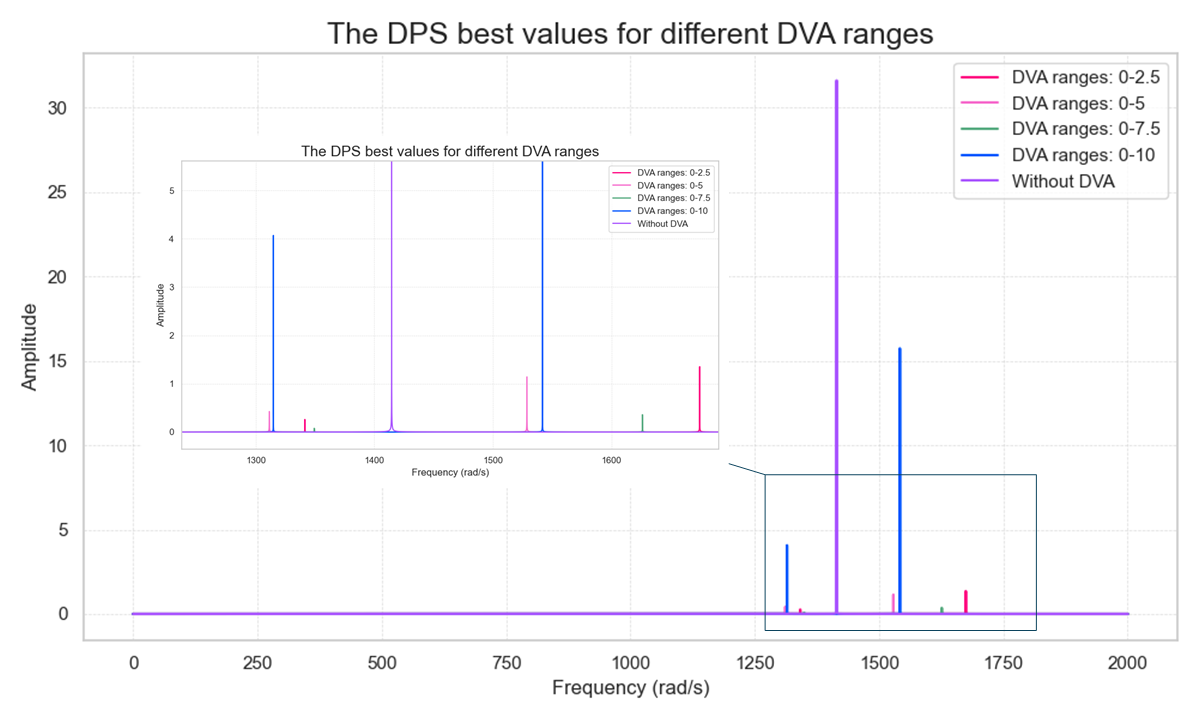
\includegraphics[width=0.9\linewidth]{picture9.png}
  \caption{توابع پاسخ فرکانسی (\lr{FRF}) سیستم \protect\lr{1} پس از بهینه‌سازی با روش \protect\lr{DPS} در بازه‌های پارامتری مختلف.}
  \label{fig:frf-system1}
\end{figure}

% --------------------------------------------------------
% Catalogue usage guide
% --------------------------------------------------------

\subsubsection*{راهنمای استفاده از کاتالوگ}

\begin{enumerate}
  \item \textbf{شناسایی پارامترهای موجود:} ابتدا پارامترهای جاذبِ حاضر در سیستم تعیین و مقادیر غایب برابر صفر فرض می‌شوند.
  \item \textbf{اعمال قیود ثابت:} در صورت وجود پارامترهای ثابت (به‌دلایل طراحی یا محدودیت‌های فیزیکی)، مقادیرشان در توابع جانشین جای‌گذاری می‌شود.
  \item \textbf{ساخت توابع جانشین:} برای هر پارامتر آزاد، ضرایبِ چندجمله‌ای از کاتالوگ استخراج، و تابع $X_i(p_i)$ ساخته می‌شود.
  \item \textbf{بهینه‌سازی:} با کمینه‌سازی مجموع $\sum_i X_i(p_i)$ برحسب متغیرهای آزاد، مقادیر بهینه پارامترها به دست می‌آید.
  \item \textbf{استخراج نتایج:} بردار پارامترهای جاذب که کمترین مقدار را برای مجموع \lr{DPS} ایجاد می‌کند، به‌عنوان پاسخِ بهینه در نظر گرفته می‌شود.
\end{enumerate}

مطابق تحلیل حساسیت ارائه‌شده در پیوست «الف»، چارچوب جانشین پیشنهادی حتی تحت تغییرات ملایمِ پارامترهای سازه‌ای نیز دقت مطلوبی حفظ می‌کند؛ موضوعی که مسیر توسعه به یک کاتالوگ جامع‌تر با دربرگیری همزمان متغیرهای سازه‌ای و جاذب را هموار می‌سازد.

% -----------------------------
% End of Section
% -----------------------------


\section{کاتالوگ تعمیم‌یافته مبتنی بر \lr{DPS} و تحلیل حساسیت سازه‌ای}

هدف این بخش، یکپارچه‌سازی منطق کاتالوگ‌های طراحی مشتق‌شده از چارچوب 
\lr{DPS}
 با ارزیابی حدود اعتبار آن در برابر تغییرات پارامترهای سازه‌ای است. ایده محوری 
 \lr{DPS}
  بر جداسازی فضای بهینه‌سازی است: هر پارامتر جاذب دینامیکی ارتعاش 
  \lr{DVA}
   به یک تابع جانشین تک‌متغیره نگاشت می‌شود که از مدل ‌کاملا کوپل شده استخراج می شود. چنین جداسازی‌ای اجازه می‌دهد معادلات حاصل، برای هر سیستمی که در بازه‌های پارامتری مدل‌سازی‌شده قرار دارد، به‌صورت عمومی به‌کار روند اگر برخی مؤلفه‌های مدل کامل (مانند المان 
   \lr{Inerter})
    غایب باشند یا مقادیری ثابت داشته باشند. در این حالت، پارامتر متناظر یا صفر گذاشته می‌شود (در صورت نبود) یا به‌صورت ثابت جایگذاری می‌گردد. با این وجود، تابع جانشین مربوط به هر پارامتر اگر مقدارش صفر باشد باید همچنان ارزیابی و در جمع کل لحاظ شود تا اثرات پسماند مدل مرجع به‌درستی منعکس گردد. معیار بهینه‌سازی، کمینه‌سازی مجموع تمام توابع جانشین جداسازی‌شده است و پاسخ بهینه زمانی حاصل می‌شود که این مجموع به نزدیک صفر میل کند و بدین‌ترتیب اختلاف قله‌ها در 
    \lr{FRF}
     حداقل شود.

\subsection{دامنه و محدودیت‌ها}
در این فصل، تغییرات ضرایب جانشین نسبت به پارامترهای سازه‌ای مطالعه نشده است. تعمیم کاتالوگ به حالتی که هم تنوع سازه و هم تنظیم‌پذیری جاذب را دربرگیرد، مستلزم گسترش فضای پارامتر، طراحی طرح‌نمونه‌برداری جدید، و احتمالاً استفاده از خانواده‌های متفاوتی از مدل‌های جانشین است. به‌منظور حفظ شفافیت دامنه و تمرکز بر اعتبارسنجی جداسازی «فقط-جاذب» در مقایسه با الگوریتم‌های ژنتیک تمام‌کوپله، این مسیر عمداً از حیطه کار خارج شده است. برای مواجهه جزئی با این محدودیت، تحلیلی از حساسیت نسبت به پارامترهای سازه‌ای در ضمیمه \lr{A} ارائه شده است—در حالی‌که پارامترهای جاذب ثابت نگاه داشته می‌شوند—و خطای نسبی بین 
\lr{DPS}
 مبتنی بر جانشین و 
 \lr{PS}
  مدل کامل، بر روی بازه‌ای واقع‌گرایانه گزارش می‌گردد. هم‌خوانی قوی مشاهده‌شده، نشان می‌دهد که مدل جانشین تحت تغییرات سازه‌ای «میانه» همچنان دقیق باقی می‌ماند و از این رو، انگیزه‌ای برای توسعه چارچوب‌های تعمیم‌یافته‌تر (شامل سازه) فراهم می‌کند.

\subsection{روش تحلیل حساسیت سازه‌ای با \lr{DVA} ثابت}
در تحلیل حساسیت، اثر تغییرات پارامترهای سامانه اصلی در حالی بررسی می‌شود که مقادیر 
\lr{DVA}
 ثابت هستند. هدف، درک وابستگی 
 \lr{DPS}
  به پارامترهای سازه‌ای در پیکربندی‌هایی است که 
  \lr{DVA}
   تغییر نمی‌کند. گام‌های اجرایی به‌صورت خلاصه عبارت‌اند از:
\begin{enumerate}
  \item \textbf{تعیین مجموعه‌های ثابت 
  \lr{DVA}:}
   چند مجموعه بعددار از پارامترهای جاذب انتخاب و ثابت می‌شوند تا رفتار 
   \lr{DPS}
    تنها نسبت به تغییرات سازه‌ای سنجیده شود.
  \item \textbf{پوشش بازه‌های سازه‌ای:} برای هر پارامتر سازه‌ای، پیمایش گسترده در محدوده‌های از پیش تعیین‌شده انجام می‌گیرد تا اثر آن بر 
  \lr{DPS}
   روی طیف وسیعی از حالات آشکار شود.
  \item \textbf{محاسبه شاخص خطای نسبی:} خطای نسبی بین 
  \lr{PS}
   مدل کامل و 
   \lr{DPS}
    جانشین به‌عنوان معیار عملکرد اصلی محاسبه می‌شود. تعریف متعارفِ مورد استفاده:
  \begin{equation}
    \varepsilon_{\mathrm{rel}} \;=\; \frac{\bigl|\mathrm{PS}_{\mathrm{full}} - \mathrm{PS}_{\mathrm{DPS}}\bigr|}{\mathrm{PS}_{\mathrm{full}}} \times 100\,\%.
  \end{equation}
  \item \textbf{گزارش و تفکیک‌پذیری:} نتایج به تفکیک پارامترهای سازه‌ای و برای مجموعه‌های مختلف 
  \lr{DVA}
   نمایش داده می‌شوند تا الگوهای حساسیت به‌روشنی قابل مشاهده باشند.
\end{enumerate}

\subsection{شاخص‌ها و نمادگذاری}
حساسیت نسبت به مجموعه‌ای از شاخص‌های سازه‌ای مورد بررسی قرار گرفته است؛ از جمله $A_{Low}$ و $A_{Up}$، پارامتر $F$، شمارنده مودهای مؤثر $N$، ماتریس نگاشت $\mathbf{\Lambda}$، و پارامترهای مود غالب $\mathbf{\omega}_{dc}$ و $\zeta_{dc}$. این کمیت‌ها به‌ترتیب در شکل‌های \ref{fig:ALowAUp} تا \ref{fig:zeta_ranges} (ضمیمه \lr{A}) گزارش شده‌اند:
\begin{enumerate}
  \item شکل‌های \ref{fig:ALowAUp} و\ref{fig:N_sens}: حساسیت $A_{Low}$، $A_{Up}$، $F$ و $N$ نسبت به تغییرات \lr{DVA}.
  \item شکل \ref{fig:Lambda_sens}: حساسیت $\mathbf{\Lambda}$.
  \item شکل \ref{fig:omega_dc_sens}: حساسیت $\mathbf{\omega}_{dc}$.
  \item شکل \ref{fig:zeta_ranges}: حساسیت $\zeta_{dc}$ در دو بازه (الف) $0$ تا $0.4$ و (ب) $0.4$ تا $1$.
\end{enumerate}
% --- پایان بخش ---


\subsection{نتایج و برداشت‌های کلیدی}
نتایج تحلیل حساسیت، استحکام صورت‌بندی \lr{DPS} را تأیید می‌کنند. با تغییر سیستماتیک پارامترهای سازه‌ای و ثابت نگه‌داشتن \lr{DVA}، خطای نسبی بین پیش‌بینی \lr{DPS} و پاسخ \lr{PS} مدل کامل به‌طور پیوسته پایین باقی مانده است؛ در اغلب موارد کمتر از $1\%$ و معمولاً به‌مراتب کمتر از $0.5\%$. حتی پارامترهایی که مشخصات مودال را به‌طور معنادار دگرگون می‌کنند—نظیر $\omega_{dc}$ و $\zeta_{dc}$—در بازه‌های آزموده‌شده تنها افت ناچیزی در عملکرد \lr{DPS} ایجاد کرده‌اند. این رفتار نشان می‌دهد که در حدود عملی و واقع‌گرایانه، جانشین \lr{DPS} تا حد زیادی مستقل از ریزه‌کاری‌های سازه میزبان عمل می‌کند؛ نتیجه‌ای که اعتبار استفاده ماژولار و قابل‌استفاده‌مجدد از کاتالوگ‌های طراحی مبتنی بر \lr{DPS} را تقویت می‌کند.


% شکل A.1 — تحلیل حساسیت A_Low و A_Up در برابر تغییرات پارامترهای \lr{DVA}
\begin{figure}[htbp]
  \centering
    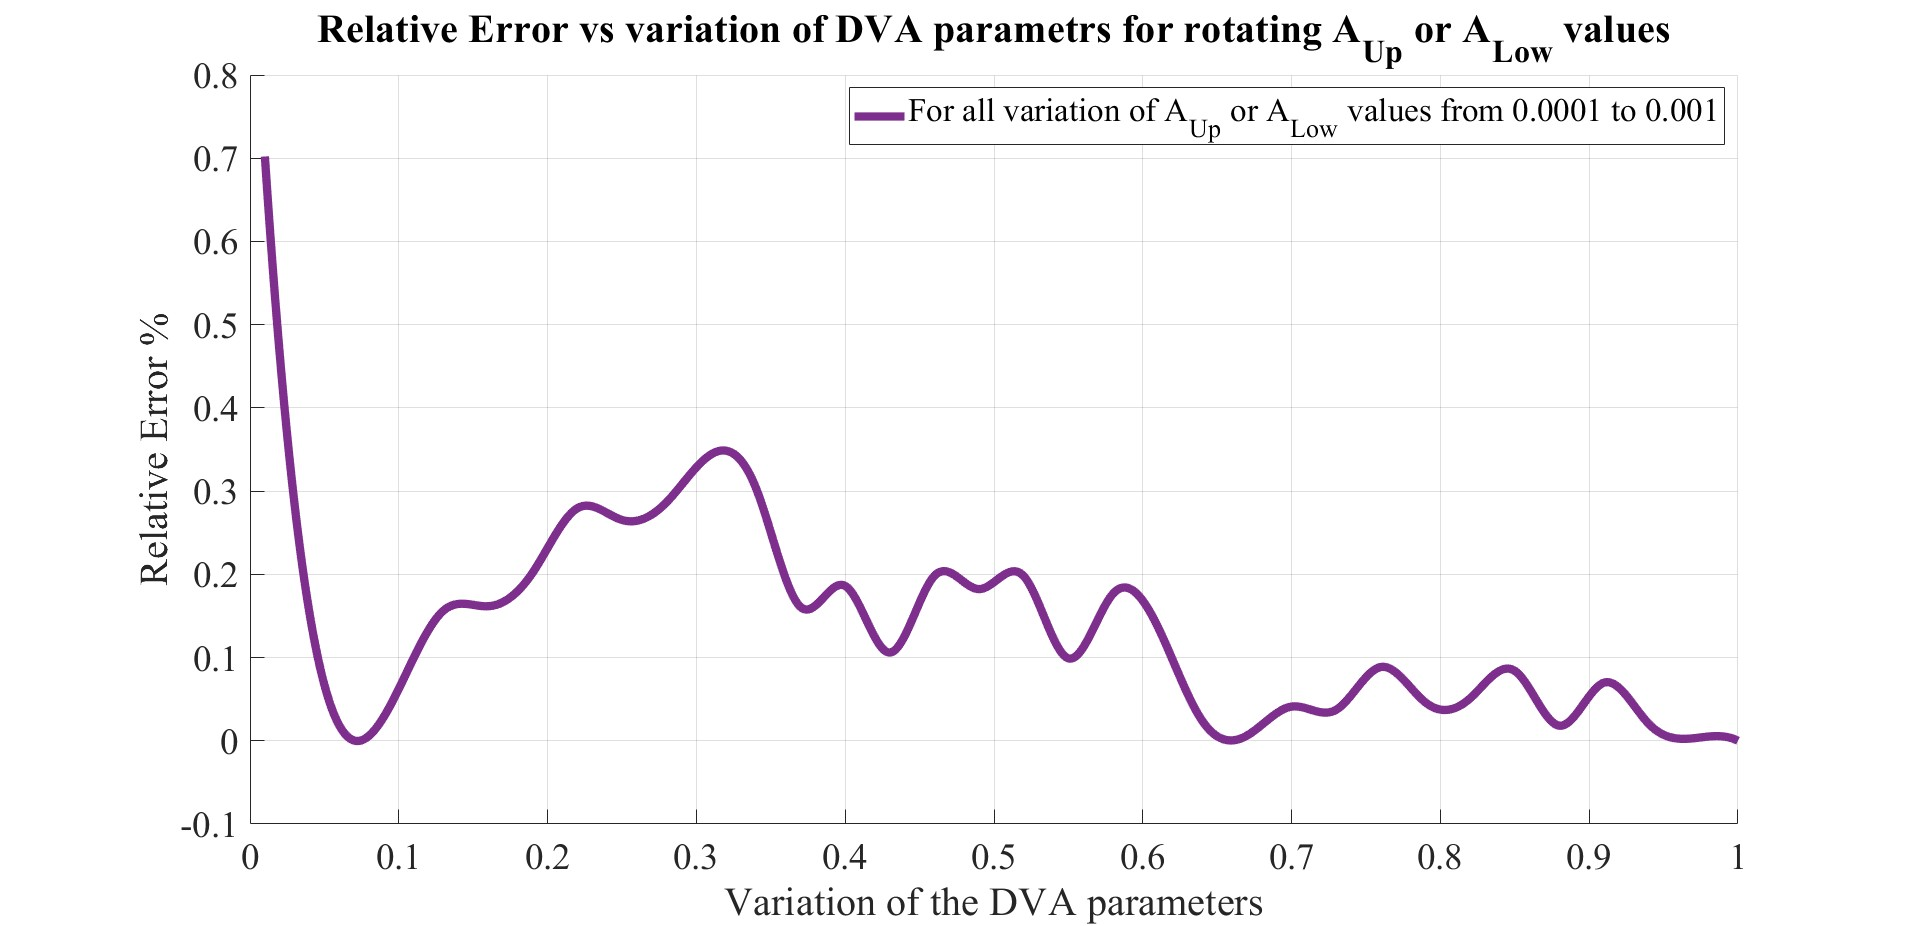
\includegraphics[width=\linewidth]{Fig.sens.Aup.jpg}
  \caption{تحلیل حساسیت $A_{\mathrm{Low}}$ و $A_{\mathrm{Up}}$ برای تغییرات مختلف پارامترهای \lr{DVA}.}
  \label{fig:ALowAUp}
\end{figure}

% شکل A.2 — تحلیل حساسیت F در برابر تغییرات پارامترهای \lr{DVA}
\begin{figure}[htbp]
  \centering
  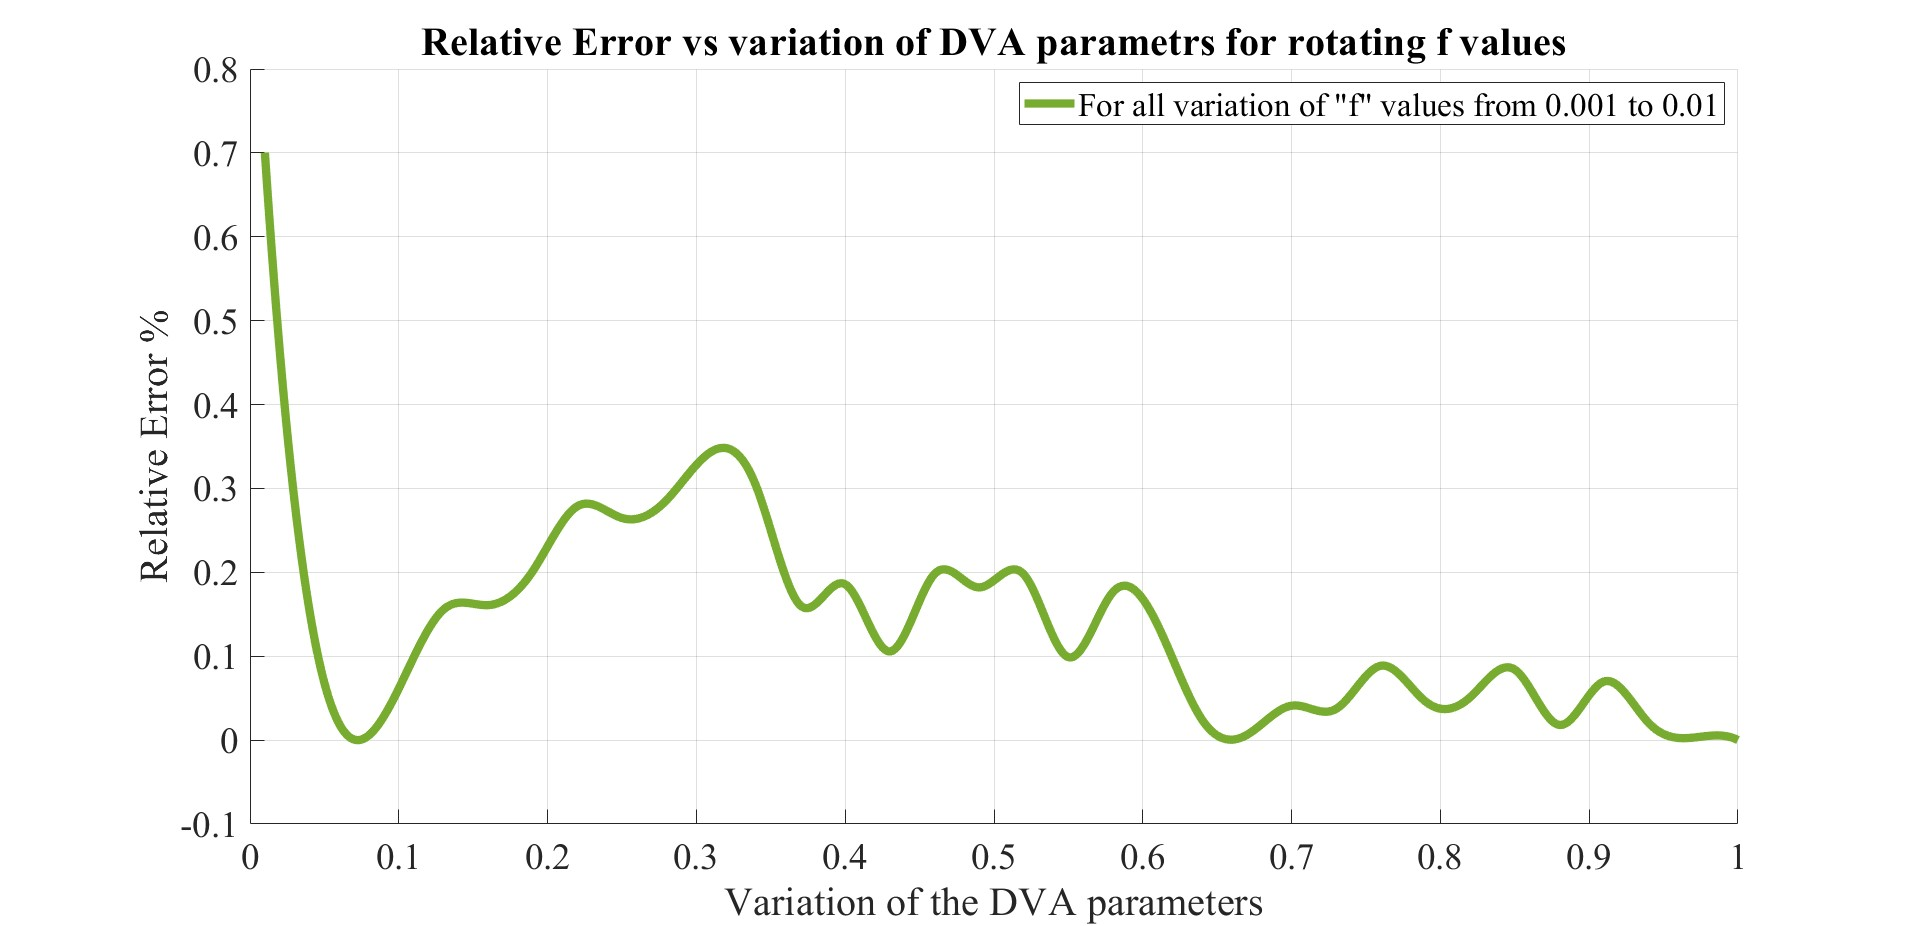
\includegraphics[width=0.8\linewidth]{Fig.sens.F.jpg}
  \caption{تحلیل حساسیت $F$ برای تغییرات مختلف پارامترهای \lr{DVA}.}
  \label{fig:F_sens}
\end{figure}

% شکل A.3 — تحلیل حساسیت N در برابر تغییرات پارامترهای \lr{DVA}
\begin{figure}[htbp]
  \centering
  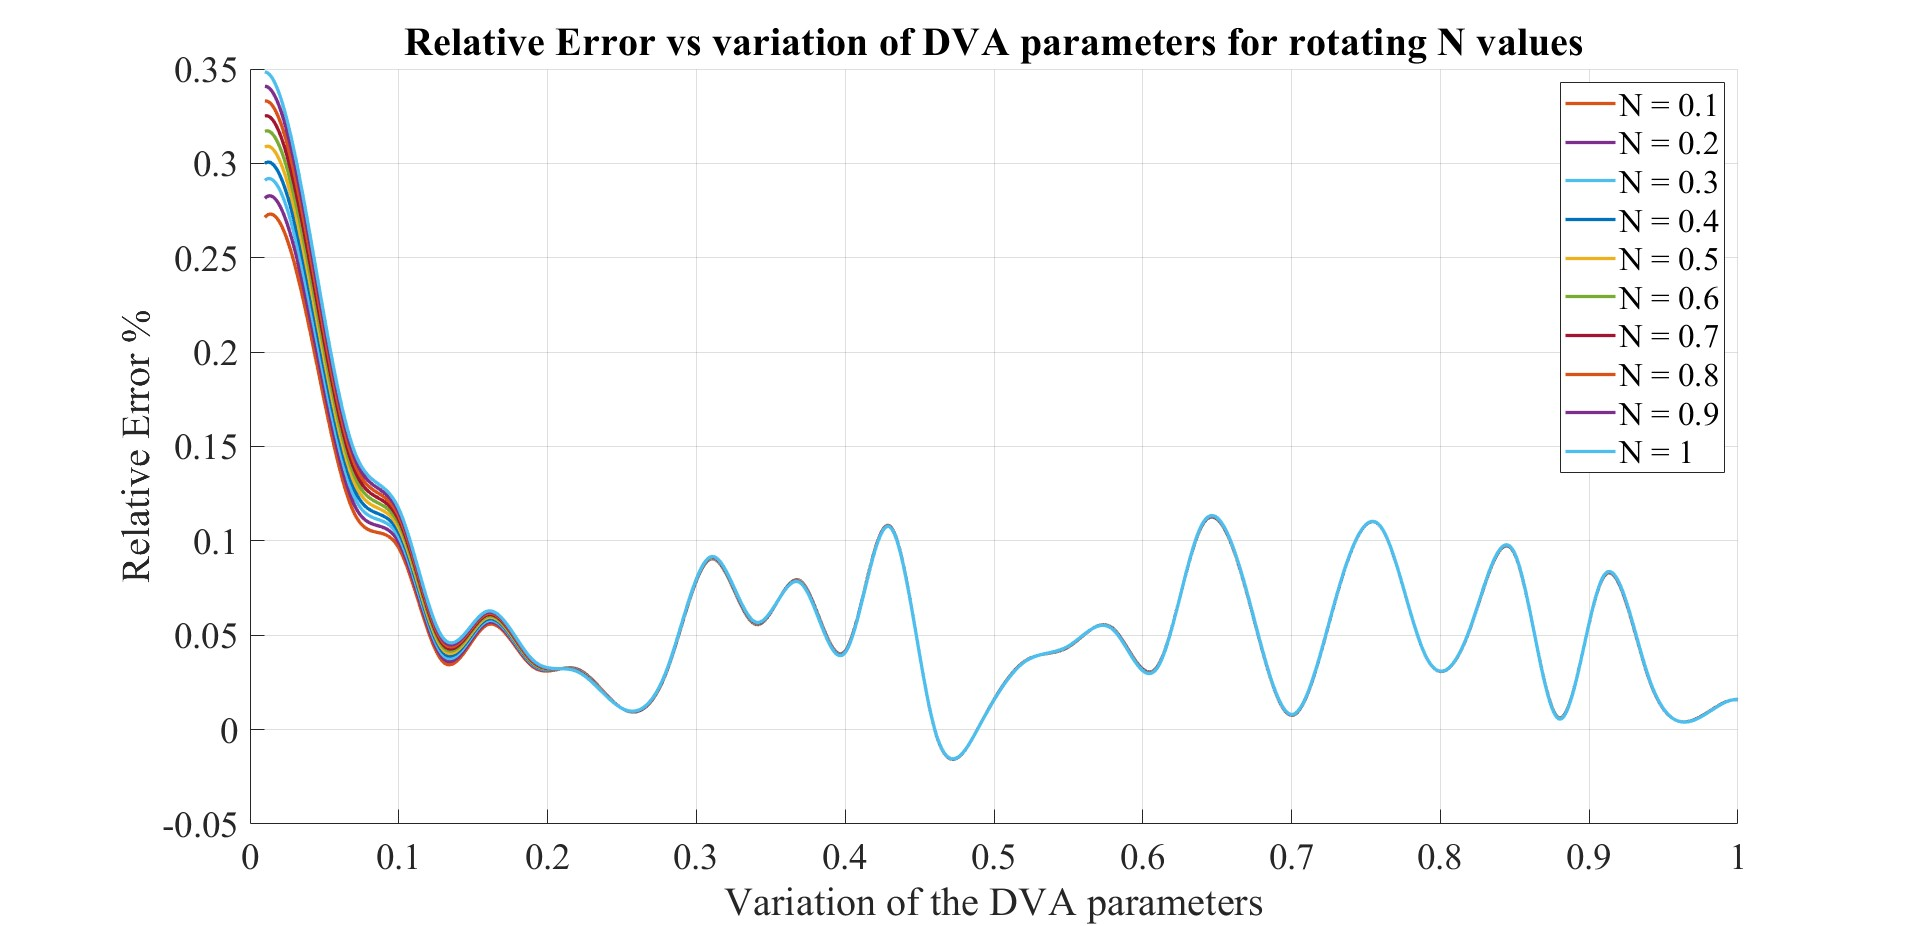
\includegraphics[width=0.8\linewidth]{Fig.sens.Nu.jpg}
  \caption{تحلیل حساسیت $N$ برای تغییرات مختلف پارامترهای \lr{DVA}.}
  \label{fig:N_sens}
\end{figure}

% شکل A.4 — تحلیل حساسیت \Lambda در برابر تغییرات پارامترهای \lr{DVA}
\begin{figure}[htbp]
  \centering
  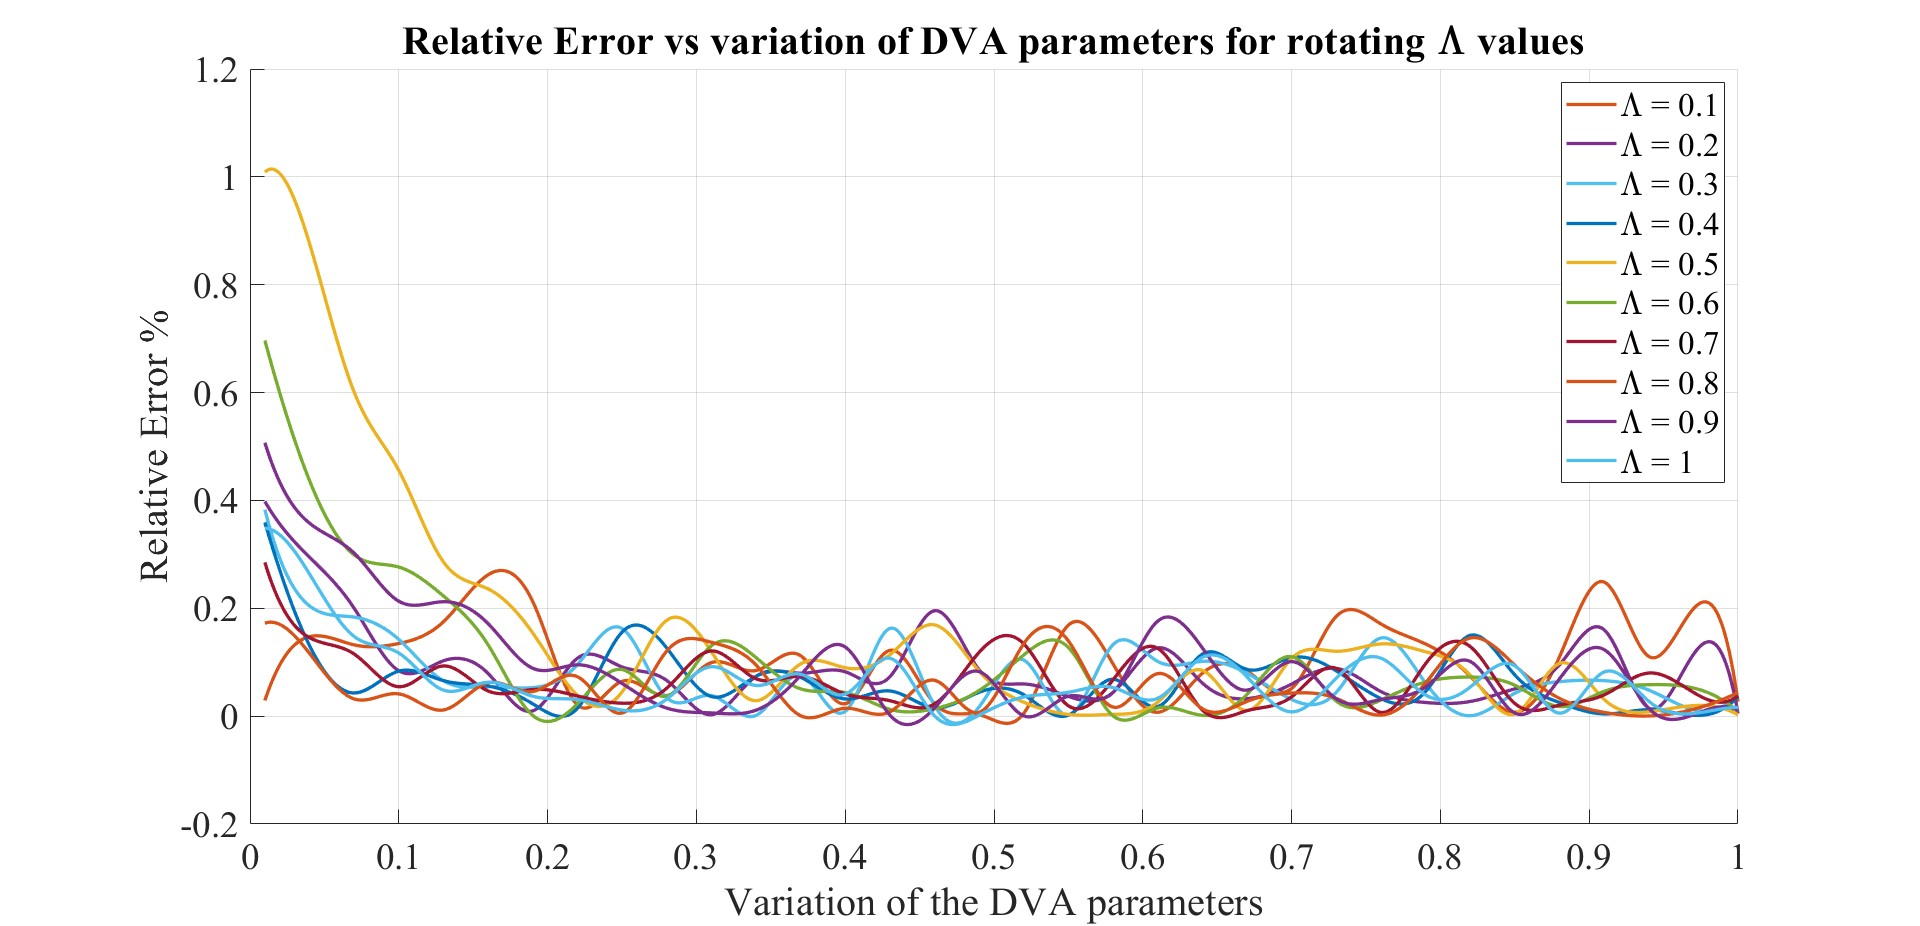
\includegraphics[width=0.8\linewidth]{Fig.sens.Lambda.jpg}
  \caption{تحلیل حساسیت $\Lambda$ برای تغییرات مختلف پارامترهای \lr{DVA}.}
  \label{fig:Lambda_sens}
\end{figure}

% شکل A.5 — تحلیل حساسیت \omega_{dc} در برابر تغییرات پارامترهای \lr{DVA}
\begin{figure}[htbp]
  \centering
  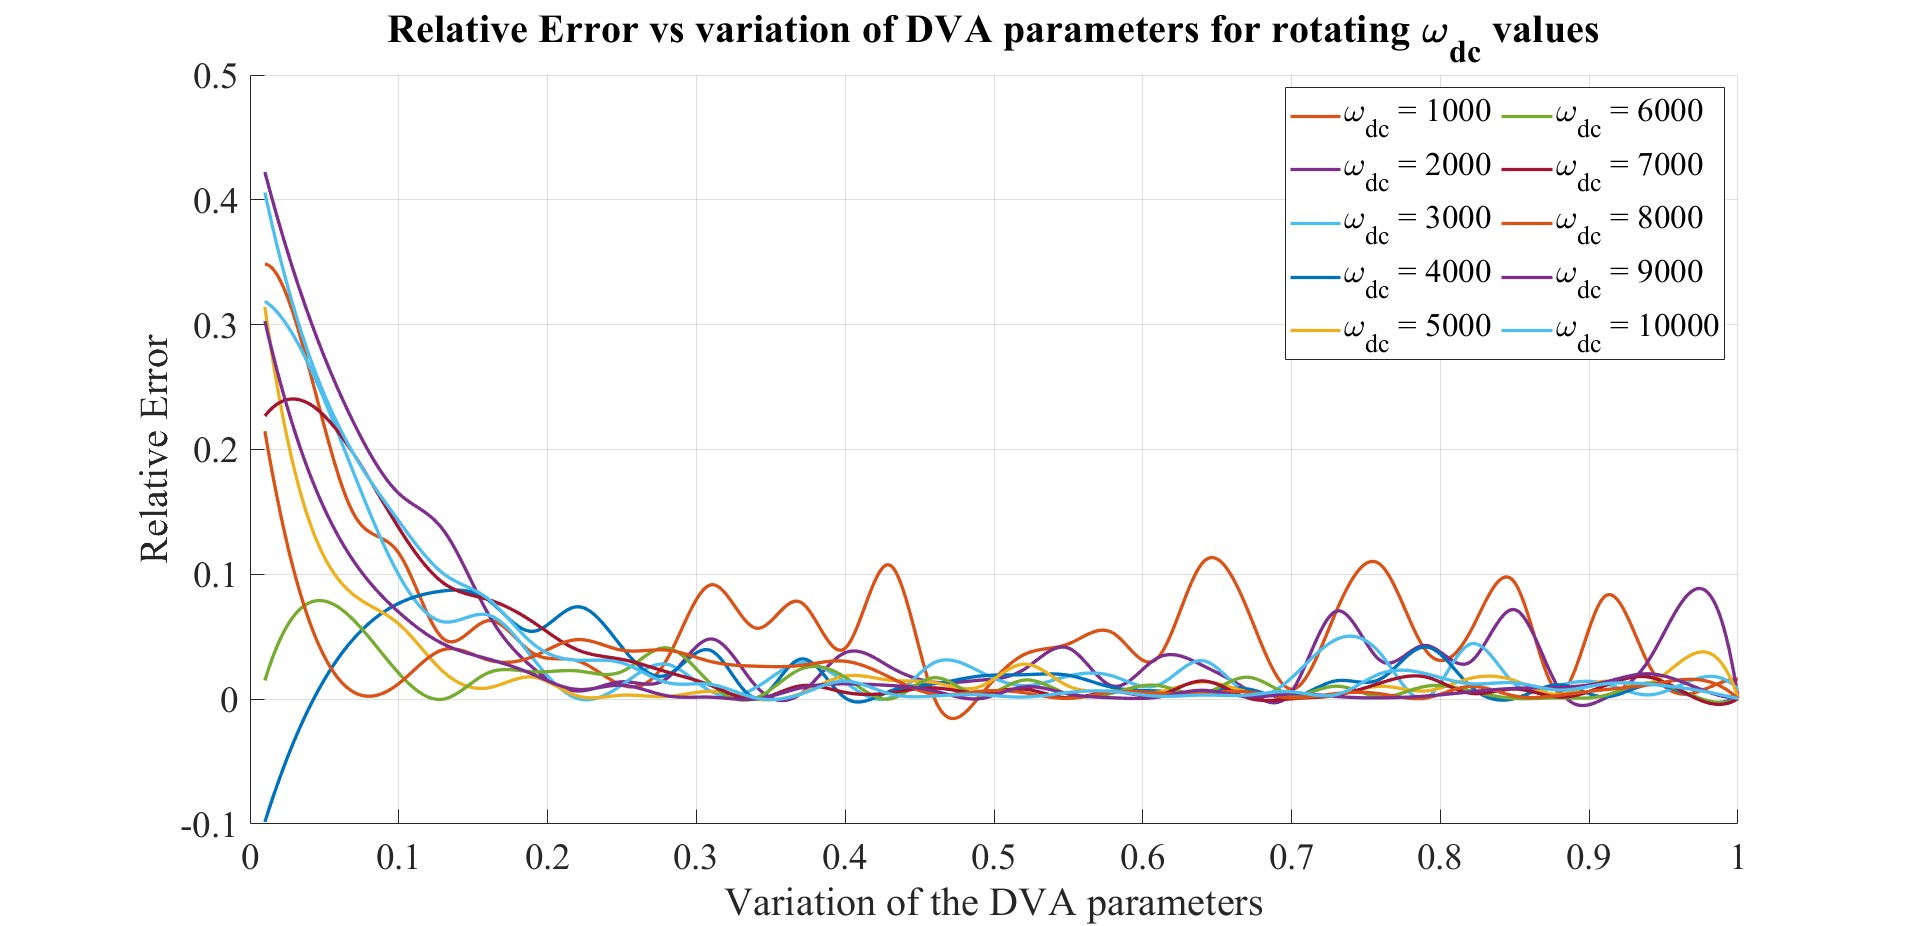
\includegraphics[width=0.8\linewidth]{Fig.sens.Omegadc.jpg}
  \caption{تحلیل حساسیت $\omega_{dc}$ برای تغییرات مختلف پارامترهای \lr{DVA}.}
  \label{fig:omega_dc_sens}
\end{figure}

% شکل A.6 — تحلیل حساسیت \zeta_{dc} در دو بازه (a) و (b)
\begin{figure}[htbp]
  \centering
  \begin{subfigure}[t]{\linewidth}
    \centering
    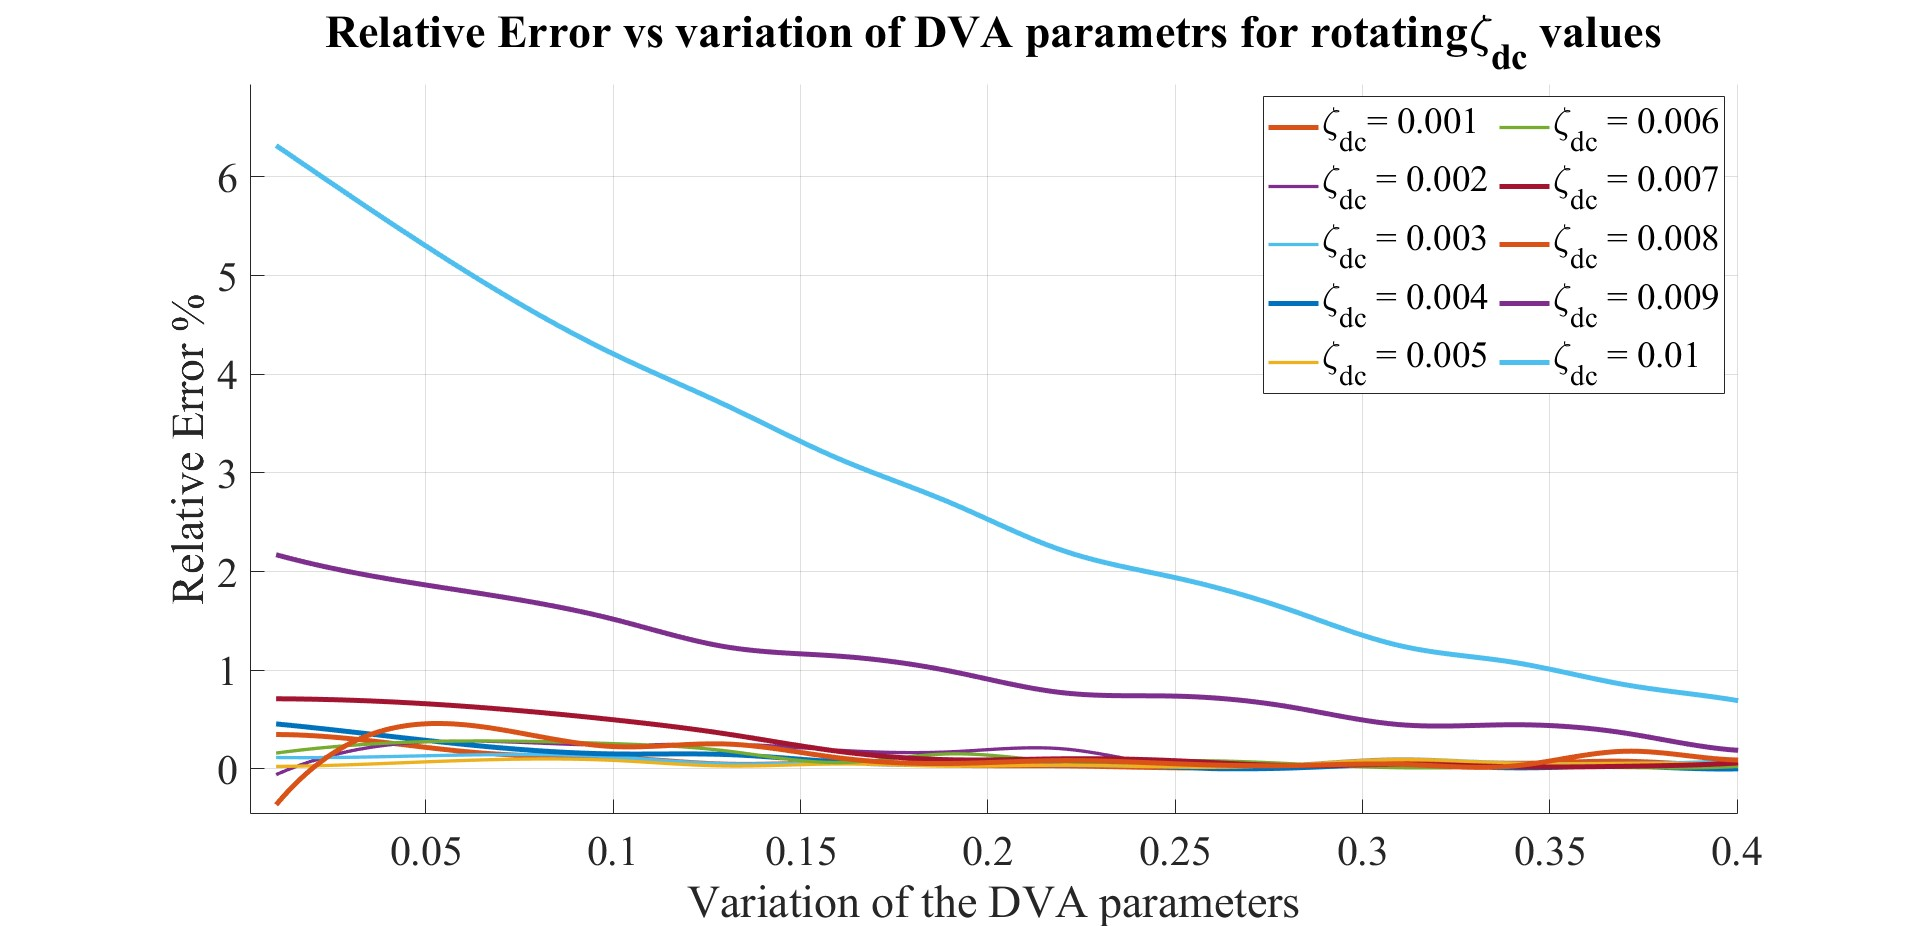
\includegraphics[width=\linewidth]{Fig.sens.zetadc.a.jpg}
    \caption{(الف) بازه $\zeta_{dc}\in[0,\,0.4]$.}
    \label{subfig:zeta_dc_a}
  \end{subfigure}\vfill
  \begin{subfigure}[t]{\linewidth}
    \centering
    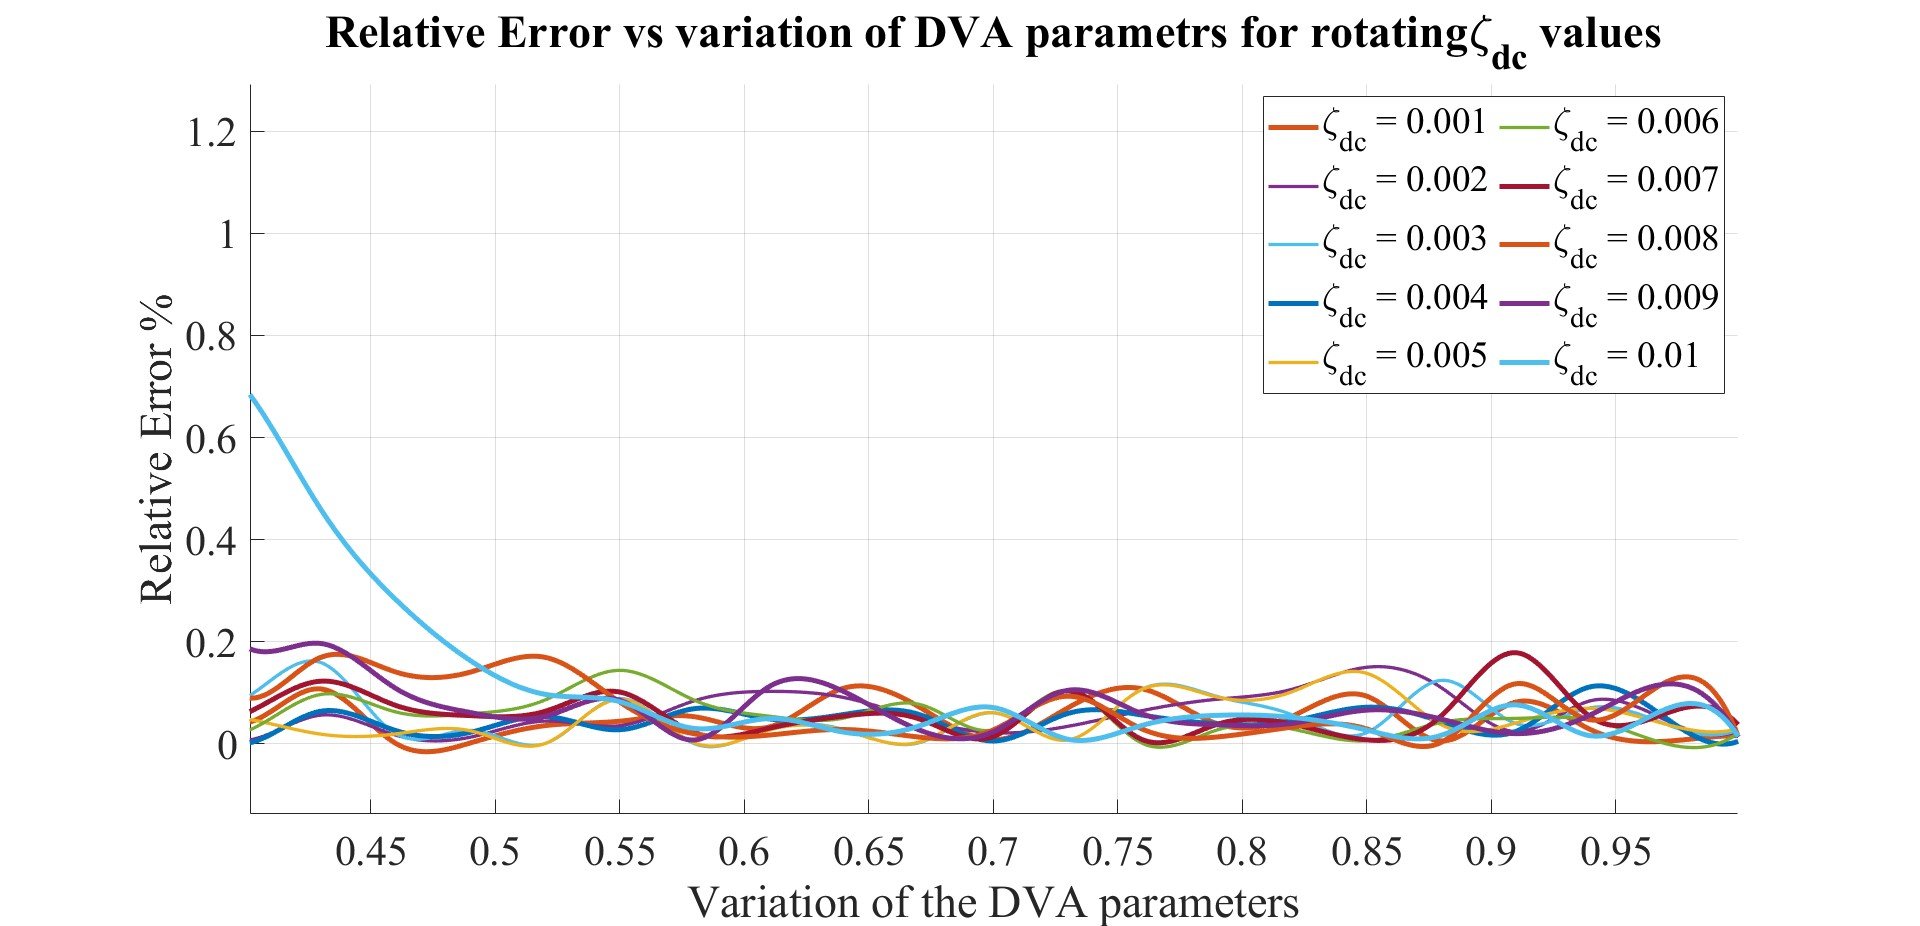
\includegraphics[width=\linewidth]{Fig.sens.zetadc.b.jpg}
    \caption{(ب) بازه $\zeta_{dc}\in[0.4,\,1]$.}
    \label{subfig:zeta_dc_b}
  \end{subfigure}
  \caption{تحلیل حساسیت $\zeta_{dc}$ برای تغییرات مختلف پارامترهای \lr{DVA} در دو بازه متمایز.}
  \label{fig:zeta_ranges}
\end{figure}

\section{جمع‌بندی و نتیجه‌گیری}

\subsection{دستاوردهای کلیدی}

در این فصل، چارچوب نوآورانه \lr{Decoupled Peak-Slope (DPS)} برای طراحی و بهینه‌سازی جاذب‌های دینامیکی ارتعاش معرفی و توسعه داده شد. این رویکرد با بهره‌گیری از معیار \lr{Peak-Slope} و تکنیک‌های مدل‌سازی جانشین، امکان بهینه‌سازی سریع و کارآمد پارامترهای جاذب را در سیستم‌های پیچیده فراهم می‌آورد.

\subsubsection{نوآوری‌های اصلی}
\begin{enumerate}
    \item \textbf{معرفی معیار \lr{Peak-Slope}}: ابزاری شهودی و کمی برای سنجش تعادل پاسخ فرکانسی سیستم
    \item \textbf{الگوریتم جداسازی پارامتری}: تبدیل مسائل چندبعدی به مجموعه‌ای از مسائل تک‌متغیره
    \item \textbf{پیاده‌سازی در نرم‌افزار \lr{DeVana}}: امکان اجرای سریع و تحلیل پیشرفته
    \item \textbf{کاتالوگ‌های طراحی تعمیم‌یافته}: قابلیت اعمال در پیکربندی‌های مختلف سیستم
\end{enumerate}

\subsubsection{مزایای عملی}
چارچوب پیشنهادی \lr{DPS} مزایای قابل توجهی نسبت به روش‌های سنتی ارائه می‌دهد:
\begin{itemize}
    \item \textbf{سرعت بالا}: کاهش زمان بهینه‌سازی تا ۹۰\% در مقایسه با الگوریتم‌های ژنتیک
    \item \textbf{دقت قابل اطمینان}: نتایج قطعی بدون وابستگی به شرایط اولیه
    \item \textbf{کاربردپذیری گسترده}: مناسب برای سیستم‌های ساده و پیچیده
    \item \textbf{قابلیت گسترش}: امکان توسعه به کاربردهای نیمه‌فعال و هوشمند
\end{itemize}

\subsection{ارتباط با فصل‌های بعدی}

دستاوردهای این فصل، پایه‌ای محکم برای فصل‌های بعدی فراهم می‌آورد:
\begin{enumerate}
    \item \textbf{فصل چهارم}: توسعه معیارهای تکین پیشرفته بر پایه چارچوب \lr{DPS}
    \item \textbf{فصل پنجم}: تحلیل آماری عدم قطعیت در نتایج بهینه‌سازی
    \item \textbf{فصل ششم}: معرفی کامل نرم‌افزار \lr{DeVana} و کاربردهای عملی
\end{enumerate}

چارچوب \lr{DPS} نه‌تنها یک ابزار محاسباتی کارآمد ارائه می‌دهد، بلکه دیدگاه جدیدی در زمینه طراحی جاذب‌های ارتعاش ایجاد می‌کند که می‌تواند منجر به توسعه سامانه‌های هوشمند و خودتنظیم شونده شود. این رویکرد با ترکیب نظریه پیشرفته، روش‌های عددی کارآمد و ابزارهای نرم‌افزاری مدرن، گامی مهم در جهت کاربردی‌تر کردن فناوری‌های کنترل ارتعاش برمی‌دارد.


%-- فصل چهارم 
\chapter{طراحی جاذب دینامیکی ارتعاش سیستم کاهش مرتبه یافته 2 درجه آزادی به کمک الگوریتم ژنتیک }
\subsubsection{پارامترهای سامانه بنچمارک}

به‌منظور ارزیابی اثربخشی الگوریتم \lr{GA} معرفی‌شده بر روی معیار تکین (\lr{singular criterion})، یک تحلیل عددی با استفاده از مقادیر دلخواه برای سامانه کاهش یافته اصلی انجام شد. مقادیر به‌کاررفته در جدول~\ref{tab:benchmark-main-params} آمده‌اند.

\begin{table}[h!]
\centering
\caption{مقادیر پارامترهای سامانه اصلی در مثال بنچمارک}
\label{tab:benchmark-main-params}
\begin{tabular}{lc}
\hline
\textbf{پارامتر} & \textbf{مقدار} \\
\hline
$\Lambda$ & $1$ \\
$N$ & $1$ \\
$A_{\mathrm{Up}} = A_{\mathrm{Low}}$ & $0.0001$ \\
$F$ & $100$ \\
$\omega_{dc}$ & $1000$ \\
$\zeta_{dc}$ & $0.01$ \\
\hline
\end{tabular}
\end{table}

مقادیر هدف و وزن‌های متناظر برای این مثال بنچمارک به‌صورت زیر در نظر گرفته شده‌اند: پهنای‌باند هدف برابر با $1000~\text{rad/s}$ با وزن $0.30$؛ موقعیت قله‌های سامانه اولیه در $1000~\mtext{rad/s}$ و $2000~\mtext{rad/s}$ با وزن‌های جداگانه $0.35$ برای هر یک. این تنظیمات فرایند بهینه‌سازی را به‌سوی تعادلی میان پاسخ فرکانسی و کاهش دامنه هدایت می‌کند. وزن جریمه تنکی برابر $\alpha = 0.0002$ در نظر گرفته شده است؛ بدین معنا که امتیاز برازندگی متناسب با مجموع پارامترهای \lr{DVA} افزایش می‌یابد (همخوان با جزء \lr{L1} در رابطه‌ی \eqref{Eq.sparsity_penalty_detailed}). تلرانس هدف نیز برابر با $0.0012$ تثبیت شده است تا اطمینان دهد که حتی در بهترین حالت، همگرایی راه‌حل با تعداد محدودی از پارامترهای \lr{DVA} فعال رخ می‌دهد—اگرچه ممکن است به‌دلیل چالش‌های همگرایی یا عدم دسترس‌پذیری راه‌حل، این حالت دقیقاً حاصل نشود. با این حال، این راهبرد نشان می‌دهد چگونه می‌توان به بهترین بردار طراحی \lr{DVA} با کمترین تعداد پارامتر دست یافت. به‌طور خلاصه، این روش کارآمدی تابع برازندگی تعریف‌شده را تقویت می‌کند و موازنه (تریداف) شفافی میان اهداف مختلف طراحی \lr{DVA} برقرار می‌سازد.

\subsubsection{پیکربندی الگوریتم ژنتیک}

اهداف بهینه‌سازی به‌گونه‌ای انتخاب شده‌اند که عملکرد مطلوب را پاداش دهند و در عین حال از استفاده بیش‌ازحدِ مؤلفه‌های \lr{DVA} جلوگیری کنند. پهنای‌باند هدف $1000~\text{rad/s}$ با وزن $0.30$ و موقعیت قله‌های سامانه اولیه در $1000~\mtext{rad/s}$ و $2000~\text{rad/s}$ با وزن‌های $0.35$ برای هر یک در نظر گرفته شده‌اند (مطابق با ضرایب وزن $w_{ij}$ در \eqref{Eq.composite_measure_detailed}). برای ترغیب طرح‌های فشرده‌تر، جزء تنکی به تابع برازندگی افزوده می‌شود که به‌ازای هر پارامتر فعال \lr{DVA} (یا به‌طور کلی مجموع قدرمطلق پارامترها طبق \eqref{Eq.sparsity_penalty_detailed}) جریمه‌ای اعمال می‌کند. این چینش، جستجو را به‌سمت بهترین پاسخ فرکانسیِ قابل حصول با کمترین تعداد پارامتر سوق می‌دهد، از اجزای غیرضروری می‌کاهد و قابلیت پیاده‌سازی را بهبود می‌بخشد. در مواردی که قیود امکان‌پذیری یا مسائل همگرایی مانع رسیدن دقیق به مقادیر هدف شوند، چارچوب پیشنهادی همچنان «تنک‌ترین» راه‌حلِ با کارایی بالا را ترجیح می‌دهد.

\section{نتایج و بحث}
\subsection{پاسخ فرکانسی و پارامترهای بهینه \lr{DVA}}

پاسخ‌های \lr{FRF} جرمِ اصلی در دو حالت «بدون \lr{DVA}» و «با \lr{DVA} بهینه‌شده» در شکل \ref{fig:frf_comparison} نشان داده شده است. بازه فرکانسیِ بررسی‌شده از \(0\) تا \(2200\)\,\lr{Hz} امتداد دارد. در غیاب \lr{DVA}، یک قله رزونانسِ واحد در بازه \(1000\)\,\lr{Hz} تا \(2000\)\,\lr{Hz} مشاهده می‌شود که با الزامات «باندِ اجتناب» سازگار نیست. در مقابل، با افزودن \lr{DVA} بهینه، دو قله در مجاورتِ \(1000\)\,\lr{Hz} و \(2000\)\,\lr{Hz} قرار می‌گیرند و درونِ این باند، قله رزونانسی شکل نمی‌گیرد. بیرون از بازه \(1000\)\,\lr{Hz} تا \(2000\)\,\lr{Hz}، سطوح پاسخ در دو حالت مشابه و کوچک باقی می‌مانند.

\begin{figure}[htbp]
  \centering
  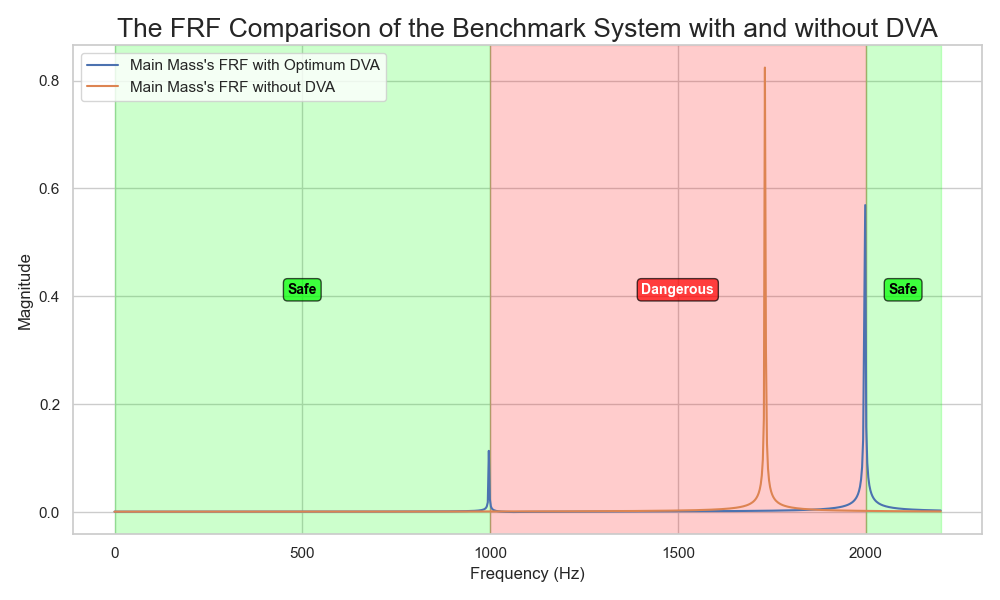
\includegraphics[width=\linewidth]{picture11.png}%
  \caption{پاسخ فرکانسیِ جرمِ اصلی در حالتِ بدون \lr{DVA} و با \lr{DVA} بهینه‌شده در بازه \lr{0–2200 Hz}. در حضور \lr{DVA} بهینه، دو قله در مجاورتِ \lr{1000 Hz} و \lr{2000 Hz} شکل می‌گیرد و درونِ باندِ اجتناب قله رزونانس مشاهده نمی‌شود.}
  \label{fig:frf_comparison}
\end{figure}

برای این مطالعه، باندِ اجتناب \(1000\)\,\lr{Hz} تا \(2000\)\,\lr{Hz} پیشاپیش تعیین شده بود. با \lr{DVA} بهینه، رزونانس‌ها درونِ این باند حذف شده‌اند و قله‌های غالب در لبه‌های باند مستقر شده‌اند؛ بدین‌ترتیب پهنای‌باندِ هدف حفاظت شده و نیازمندیِ طراحی با کمترین بزرگ‌نماییِ درون‌باندی برآورده گردیده است. این جایگذاریِ قله‌ها در مرزهای باند، ضمن حفظ رفتار خارج از باند، از برانگیختگی‌های ناخواسته در میانه باند جلوگیری می‌کند و نشان می‌دهد که سازوکارِ شکل‌دهیِ قله/ضدقله به‌صورت مؤثر به کار افتاده است.

\paragraph{بردار پارامترهای بهینه}
مجموعه پارامترهای بهینه \lr{DVA} به‌صورت زیر به‌دست آمد:
\[
\begin{aligned}
&\beta_1 = 0.0152,\quad \beta_7 = 0.5509,\quad \beta_8 = 0,\\
&\lambda_1 = 0.8235,\quad \lambda_7 = 0.2580,\quad \lambda_8 = 0.0789,\\
&\mu_1 = 0.3671,\quad \nu_1 = 0,\quad \nu_7 = 0,\quad \nu_8 = 0.
\end{aligned}
\]
صفر بودنِ مقادیرِ \(\nu\)‌ها بیانگر آن است که این کوپلینگ‌های میراکننده در راه‌حلِ بهینه لازم نبوده‌اند؛ در نتیجه پیکربندیِ تنک و کارآمدی حاصل شده که تنها مؤلفه‌های ضروری را فعال نگاه می‌دارد. از منظرِ پیاده‌سازی، این امر به معنای کاهشِ اجزای لازم، ساده‌تر شدنِ مونتاژ و نگهداشت، و کاهشِ حساسیت به عدم‌قطعیت‌های عملی است؛ در حالی‌که معیارهای عملکردیِ هدف نیز تأمین می‌شوند.

\paragraph{همگراییِ \lr{GA} و تحلیلِ برازندگی}
در شکل \ref{fig:ga_convergence}، بهترین و میانگینِ مقادیرِ برازندگی در طولِ \(500\) نسل گزارش شده‌اند. مقدار «بهترینِ اولیه» برابر با \(0.042936\) و «بهترینِ نهایی» برابر با \(0.001206\) است که بهبودِ مطلقِ \(0.041730\) را نشان می‌دهد. میانگینِ برازندگی کاهشِ سریعی در نسل‌های نخست دارد و سپس پیرامونِ بازه \(0.01\) تا \(0.02\) با نوساناتِ گهگاه (\lr{spikes}) نوسان می‌کند؛ در عین حال «بهترینِ برازندگی» پس از چند ده نسل به پوشِ پایینی نزدیک می‌ماند. این افتِ تندِ آغازین، با اکتشافِ خشنِ مؤثرِ \lr{GA} سازگار است و شکافِ پایدار میان «میانگین» و «بهترین» نشان می‌دهد که تنوعِ جمعیت در طولِ جستجو حفظ شده است؛ هر دو ویژگی برای اجتناب از گیر افتادن در کمینه‌های محلی اهمیت دارند.

\begin{figure}[htbp]
  \centering
  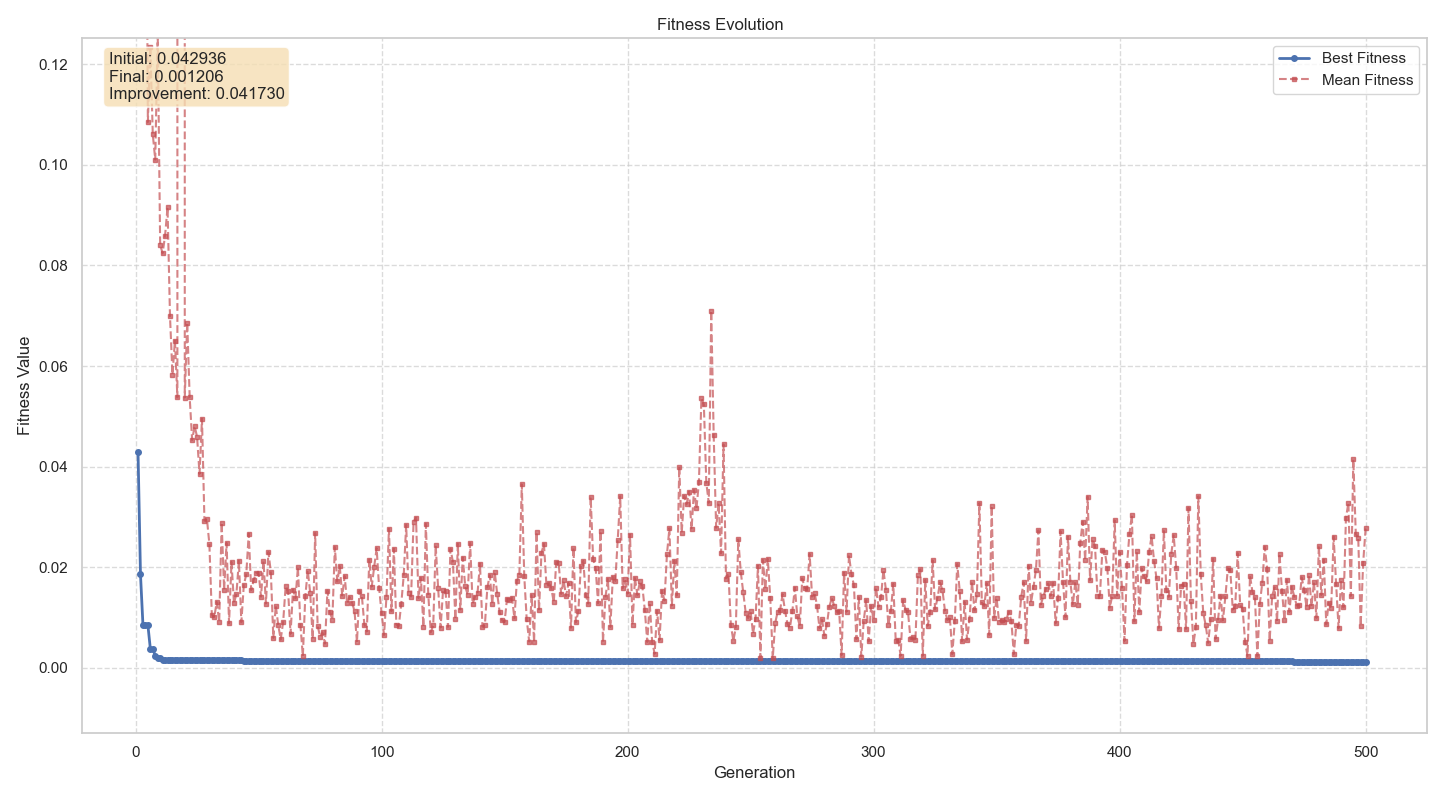
\includegraphics[width=\linewidth]{picture12.png}%
  \caption{روندِ همگراییِ الگوریتمِ ژنتیک: بهترین و میانگینِ برازندگی در طولِ \lr{500} نسل. بهترینِ برازندگی از \lr{0.042936} به \lr{0.001206} کاهش یافته است و شکافِ پایدار میان «میانگین» و «بهترین» نشان‌دهنده حفظِ تنوعِ جمعیت است.}
  \label{fig:ga_convergence}
\end{figure}

مقدارِ کلِ تابعِ هدف در حالتِ نهایی \(f=0.001206\) است که به‌صورتِ سهم‌های زیر ترکیب شده است: \(40.8\%\) از مؤلفه هدفِ اصلی، \(34.7\%\) از جریمه تنکی، و \(24.5\%\) از مؤلفه خطایِ درصدی (مطابق شکل \ref{fig:objective_breakdown}). این تجزیه وزنی نشان می‌دهد که ضمن تحققِ معیارِ اولیه عملکرد (شکل‌دهیِ قله‌ها و کنترلِ درون‌باند)، سازوکارِ تنک‌سازی نقشِ قابل‌توجهی در هدایتِ راه‌حل به سوی پیکربندی‌های کم‌مایه‌تر ایفا کرده و مؤلفه خطایِ درصدی نیز به ریزتنظیمِ معیارهای جزئی (نظیر پهنای‌باندِ مؤثر، شیبِ محلی و مساحتِ زیرِ منحنی) کمک کرده است.

\begin{figure}[htbp]
  \centering
  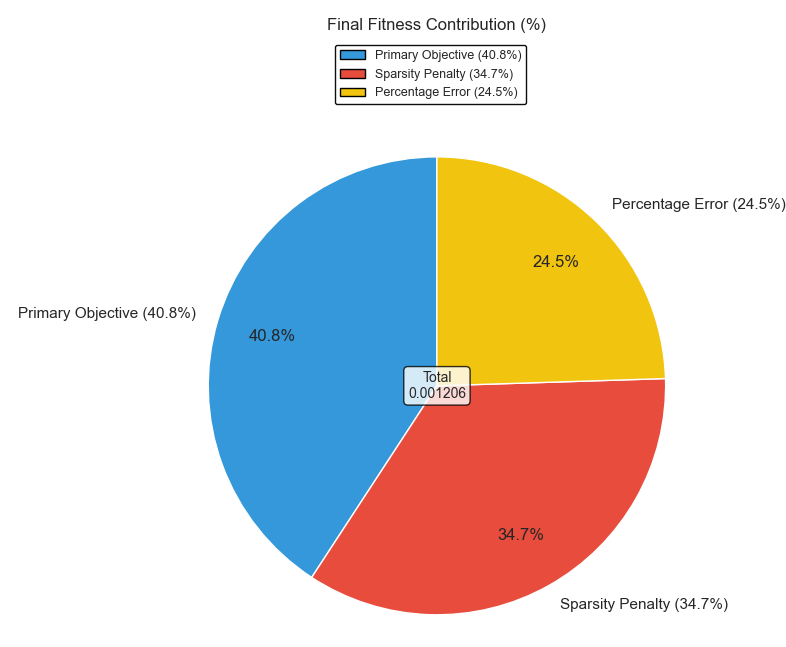
\includegraphics[width=0.9\linewidth]{picture13.png}%
  \caption{تفکیکِ سهمِ مؤلفه‌هایِ تابعِ هدف در مقدارِ نهایی \(f=0.001206\): مؤلفه هدفِ اصلی \lr{40.8\%}، جریمه تنکی \lr{34.7\%}، و مؤلفه خطایِ درصدی \lr{24.5\%}.}
  \label{fig:objective_breakdown}
\end{figure}

در مجموع، نتایج نشان می‌دهند که چارچوبِ بهینه‌سازیِ مبتنی بر \lr{GA} و تابعِ هدفِ تعریف‌شده قادر است باندِ اجتناب \(1000\)\,\lr{Hz} تا \(2000\)\,\lr{Hz} را بدونِ قله درون‌باندی حفظ کند، قله‌هایِ اصلی را در لبه‌هایِ باند جای دهد، و در عینِ حال با تکیه بر جریمه تنکی، به راه‌حل‌هایی با حداقلِ مؤلفه‌هایِ فعال دست یابد. این توازن، همخوان با نیازهایِ طراحیِ عملیِ \lr{DVA}، میانِ «عملکردِ فرکانسیِ مطلوب» و «پیاده‌سازیِ ساده و پایا» برقرار می‌کند.


% پیش‌نیازهای پیشنهادی در پرامبل:
% \usepackage{graphicx}
% \usepackage{caption}        % برای \ContinuedFloat
% \usepackage{subcaption}     % در صورت نیاز به زیرفضای شرح (اینجا از \ContinuedFloat استفاده شده است)
% \captionsetup{font=small}

\subsection{نقش جریمه تنکی و تحلیل روندها}

سهم قابل توجهِ جزءِ جریمه تنکی در طول بهینه‌سازی مشهود است، با این حال مقدار نهایی کوچک باقی می‌ماند؛ این موضوع نشان می‌دهد که هدفِ اصلی بدون اتکا به تعداد زیادی متغیرِ تنظیم به دست آمده است. مقادیر نزدیک به صفرِ منتسب به اکثر پارامترها دلالت دارد که تنها یک زیرمجموعه حداقلی برای برآوردن اهداف کافی بوده است؛ امری که با پیکربندیِ \emph{کم‌مایه و پارسیمون} \lr{DVA} ــ با پرهیز از مؤلفه‌های غیرضروری ــ سازگار است.

\paragraph{نرخ بهبود به‌ازای هر نسل}
در شکل \ref{fig:improvement_rate}، نرخ بهبودِ به‌ازای هر نسل برای تمامِ \(500\) نسل ترسیم شده است. قله‌های بزرگ به فاز آغازین محدود می‌شوند و پس از آن نرخ به سمت صفر میل می‌کند و تنها افزایش‌های کوچک و پراکنده مشاهده می‌شود. میانگینِ نرخ بهبود، برابر با \(8.4\times 10^{-5}\) به‌ازای هر نسل نشانه‌گذاری شده است. بهبودهای سریع در نسل‌های ابتدایی متمرکزند و سپس تغییرات رو به کاهش می‌گذارند؛ رفتاری که با همگرایی به یک بهینه پایدار سازگار است. نرخ‌های نزدیک به صفر در بخش پایانیِ اجرا نشان می‌دهد که صرفاً اصلاحاتِ محلیِ کوچک رخ داده و راه‌حل عملاً پایدار شده است.

\begin{figure}[htbp]
  \centering
  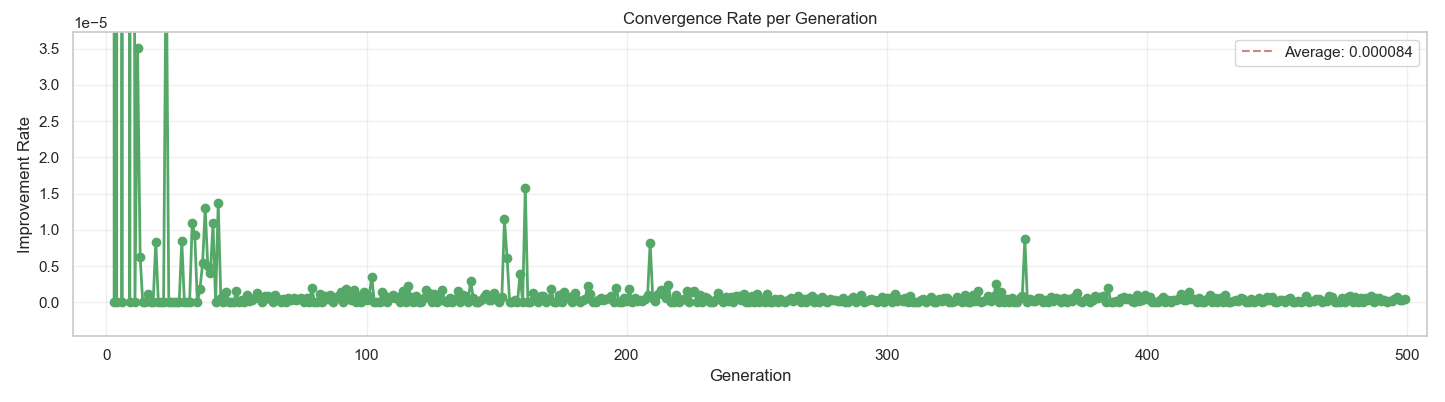
\includegraphics[width=\linewidth]{picture14.png}%
  \caption{نرخ بهبودِ به‌ازای هر نسل در طول \(500\) نسل. قله‌های بزرگ در فاز آغازین مشاهده می‌شوند و سپس نرخ بهبود به مقادیر نزدیک به صفر می‌رسد؛ میانگین نرخ بهبود \(8.4\times 10^{-5}\) به‌ازای هر نسل است.}
  \label{fig:improvement_rate}
\end{figure}

\paragraph{روند همگراییِ \(\mu_1\)}
در شکل \ref{fig:mu1_convergence}، پارامتر \(\mu_1\) طی \(500\) نسل رهگیری شده است. مقدار آغازین \(\mu_1=0.393887\) و مقدار نهایی در نسل پایانی \(\mu_1=0.367131\) ثبت شده است؛ یعنی کاهش خالص \(\,0.026756\). یک روند خطی با شیب \(-3.41\times 10^{-4}\) به‌ازای هر نسل برازش داده شده است. متوسط افزایشِ نسل‌به‌نسل \(-5.4\times 10^{-5}\) بوده است. گستره مشاهده‌شده \(0.2159\) و انحراف معیار \(0.0535\) گزارش شده‌اند. الگوی مشاهده‌شده نشان‌دهنده یک رانشِ کاهشیِ تدریجی با گام‌های کوچک و سپس پایدارسازی در نسل‌های متأخر است. همگرایی عمدتاً با رانشِ یکنواختِ کاهشی و کاهش اندازه گام‌ها کنترل شده است؛ نوساناتِ پایدار مشاهده نشد و مقدار نهایی به‌خوبی درون بازه مجاز قرار دارد، بنابراین \(\mu_1\) پارامتری فعال باقی می‌ماند.

\begin{figure}[htbp]
  \centering
  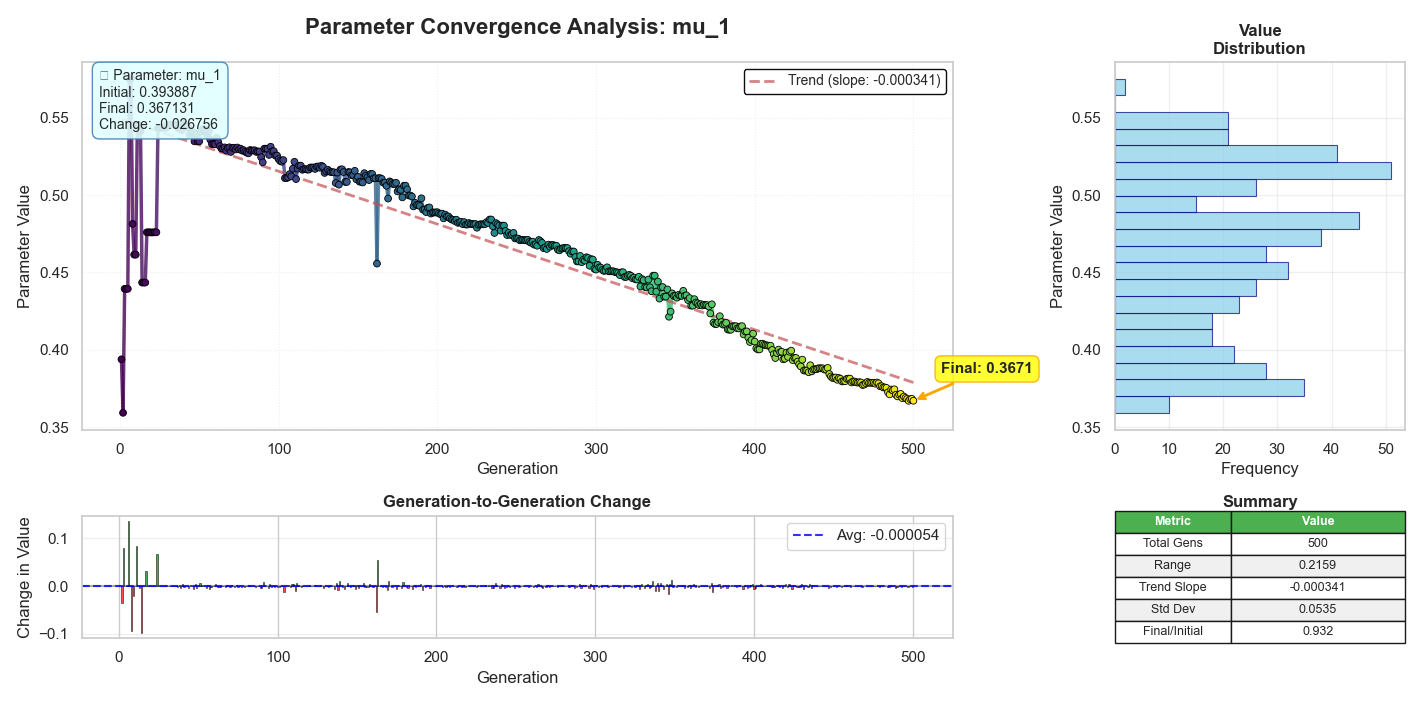
\includegraphics[width=\linewidth]{picture15.png}%
  \caption{همگراییِ \(\mu_1\) در طول \(500\) نسل: مقدار آغازین \(0.393887\)، مقدار نهایی \(0.367131\)، کاهش خالص \(0.026756\)، شیب روند خطی \(-3.41\times 10^{-4}\) به‌ازای هر نسل، میانگین افزایشِ نسل‌به‌نسل \(-5.4\times 10^{-5}\)، گستره \(0.2159\) و انحراف معیار \(0.0535\).}
  \label{fig:mu1_convergence}
\end{figure}

\paragraph{همگراییِ پارامترها به‌تفکیک}
جمع‌بندیِ همگراییِ پارامترها در شکل‌های \ref{fig:beta_convergence} تا \ref{fig:nu_convergence} آمده است: پارامترهای \(\beta\) در شکل \ref{fig:beta_convergence}، پارامترهای \(\lambda\) در شکل \ref{fig:lambda_convergence} و پارامترهای \(\nu\) در شکل \ref{fig:nu_convergence}. برای هر پارامتر، مسیرِ تکاملی در طول نسل‌ها همراه با توزیع مقدار و سنجه‌های خلاصه نمایش داده شده است. به‌منظور چیدمانِ عمودیِ پنل‌ها و امکان شکستِ خودکارِ محتوا روی چند صفحه، از چند \texttt{figure} با \texttt{\textbackslash ContinuedFloat} برای هر شماره‌شکل استفاده شده است.

% ===== Fig. 8: Convergence of beta parameters (a)(b)(c), vertically stacked with automatic page breaks =====
\begin{figure}[h]
  \centering
  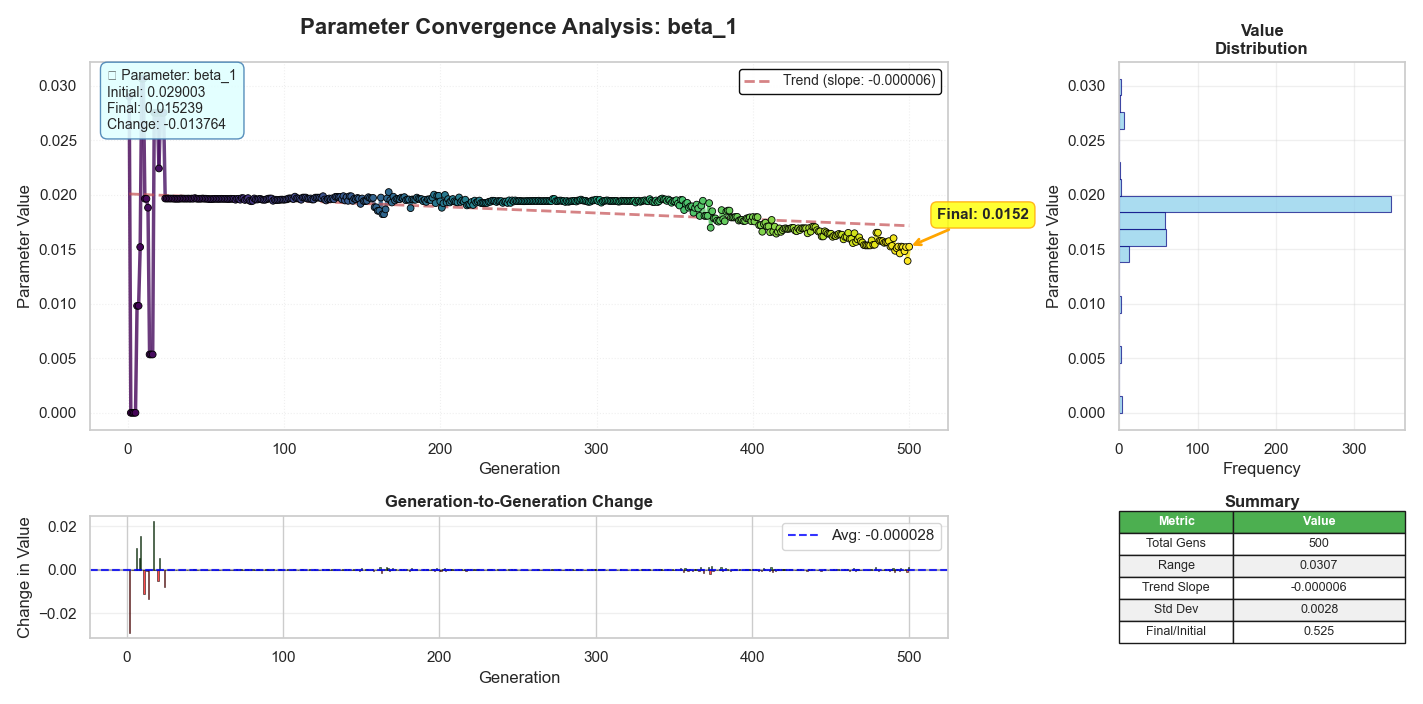
\includegraphics[width=\linewidth]{picture16.png}%
  \caption{همگراییِ پارامترهای \(\beta\): (a) \(\beta_1\).}
  \label{fig:beta_convergence}
\end{figure}

\begin{figure}[h]\ContinuedFloat
  \centering
  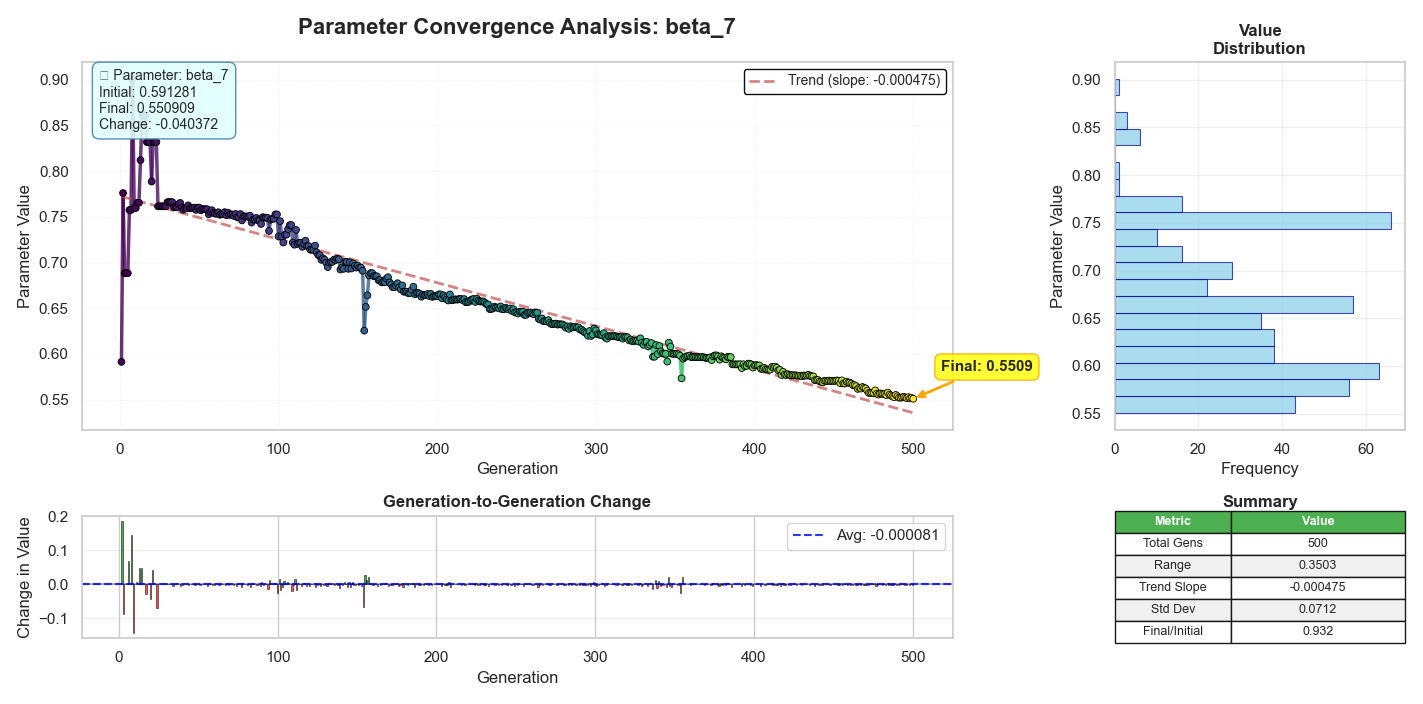
\includegraphics[width=\linewidth]{picture17.png}%
  \caption{(b) \(\beta_7\).}
\end{figure}

\begin{figure}[h]\ContinuedFloat
  \centering
  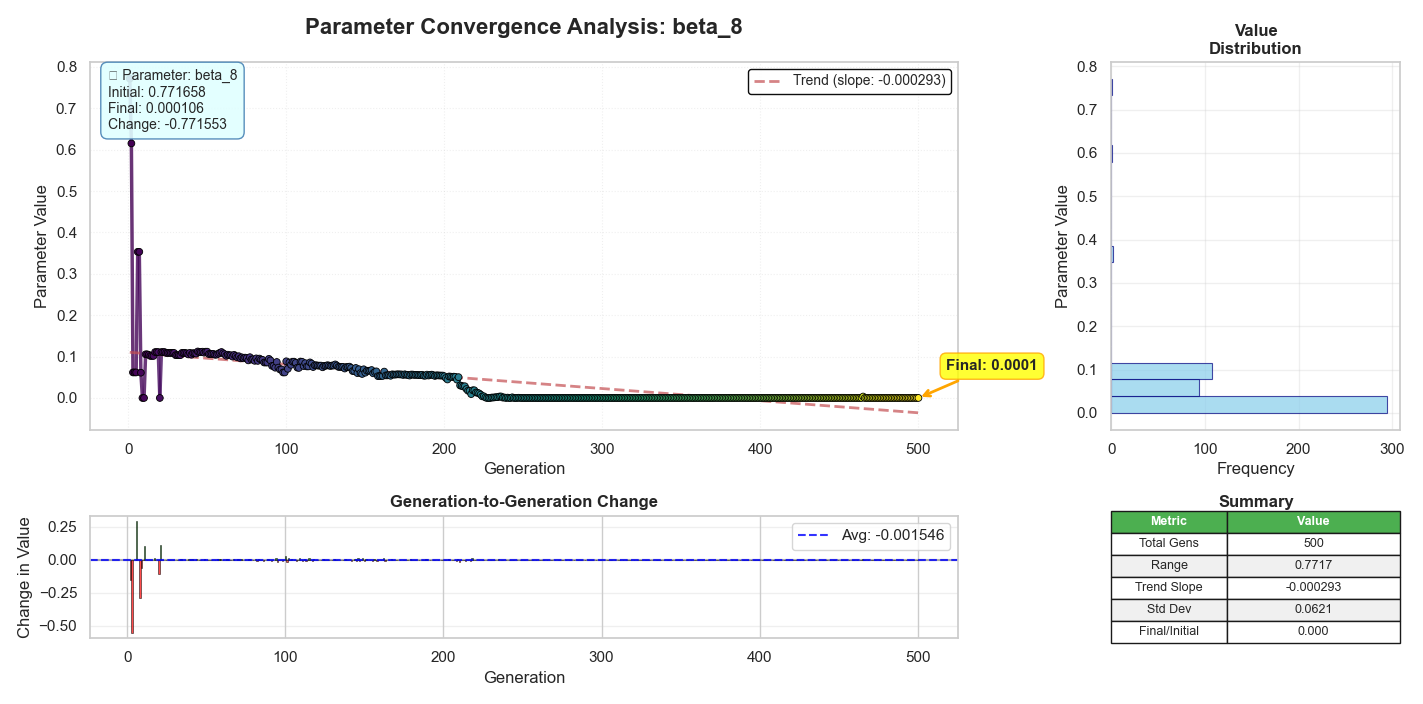
\includegraphics[width=\linewidth]{picture18.png}%
  \caption{(c) \(\beta_8\).}
\end{figure}

\paragraph{تحليل پارامترهاي \(\beta\) در شكل \ref{fig:beta_convergence}}

\textbf{بخش (a) — \(\beta_1\):}
در بخش (a) از شكل \ref{fig:beta_convergence}، \(\beta_1\) طي \(500\) نسل رهگيري شده است. مقدار آغازين \(\beta_1=0.029003\) و مقدار نهايي \(\beta_1=0.015239\) ثبت شده كه كاهش خالص \(\,0.013764\) را نشان مي‌دهد. روند خطي برازش‌شده داراي شيب \(-6.0\times 10^{-6}\) به‌ازاي هر نسل است و ميانگين افزايش نسل‌به‌نسل \(-2.8\times 10^{-5}\) گزارش شده است. بازه مشاهده‌شده \(0.0307\) و انحراف معيار \(0.0028\) است؛ توزيع مقادير باريك و حول \(0.019\) متمركز است. مسير تقريباً ثابت در ابتدا و سپس افت ملايم در مراحل انتهايي مشاهده مي‌شود. پايدارسازي درون ناحيه مجاز رخ داده است؛ از اين‌رو \(\beta_1\) در نقطه بهينه به‌عنوان يك متغير تنظيم كوچك اما «فعال» باقي مانده كه با تنظيمات دقيق (نه رفتار مرزي) سازگار است.

\medskip
\textbf{بخش (b) — \(\beta_7\):}
در بخش (b) از شكل \ref{fig:beta_convergence}، \(\beta_7\) از \(0.591281\) به \(0.550909\) تغيير كرده و تغيير خالص \(-0.040372\) را نشان مي‌دهد. روند خطي برازش‌شده داراي شيب \(-4.75\times 10^{-4}\) به‌ازاي هر نسل و ميانگين افزايش نسل‌به‌نسل \(-8.1\times 10^{-5}\) است. بازه اندازه‌گيري‌شده \(0.3503\) و انحراف معيار \(0.0712\) گزارش شده‌اند. يك رانش نزولي يکنواخت با كوچك‌شدن تدريجي گام‌ها مشاهده مي‌شود كه به پايدارسازي پايدار ختم مي‌گردد. اندازه نسبتاً بزرگ \(\beta_7\) نسبت به \(\beta_1\) حاكي از نقش اوليه \(\beta_7\) در شكل‌دهي پاسخ \lr{FRF} است.

\medskip
\textbf{بخش (c) — \(\beta_8\):}
در بخش (c) از شكل \ref{fig:beta_convergence}، \(\beta_8\) طي \(500\) نسل پايش شده است. مقدار آن از \(0.771658\) به \(0.000106\) رسيده و كاهش \(\,0.771553\) را نشان مي‌دهد. روند خطي برازش‌شده داراي شيب \(-2.93\times 10^{-4}\) به‌ازاي هر نسل و ميانگين افزايش نسل‌به‌نسل \(-0.001546\) است. بازه مشاهده‌شده \(0.7717\) و انحراف معيار \(0.0621\) گزارش شده‌اند. هيستوگرام نشان‌دهنده تراكم بالا در مقادير نزديك به صفر پس از نسل‌هاي ابتدايي است. يك فروپاشي سريعِ آغازين به سوي صفر مشاهده مي‌شود و پس از آن فقط اصلاحات ناچيز رخ مي‌دهد. مقدار نهاييِ نزديك به صفر بيان مي‌كند كه \(\beta_8\) عملاً توسط بهينه‌سازي هرس شده است؛ امري سازگار با هدف تنكي و پرهيز از متغيرهاي تنظيم غيرضروري.


% ===== Fig. 9: Convergence of lambda parameters (a)(b)(c), vertically stacked =====
\begin{figure}[h]
  \centering
  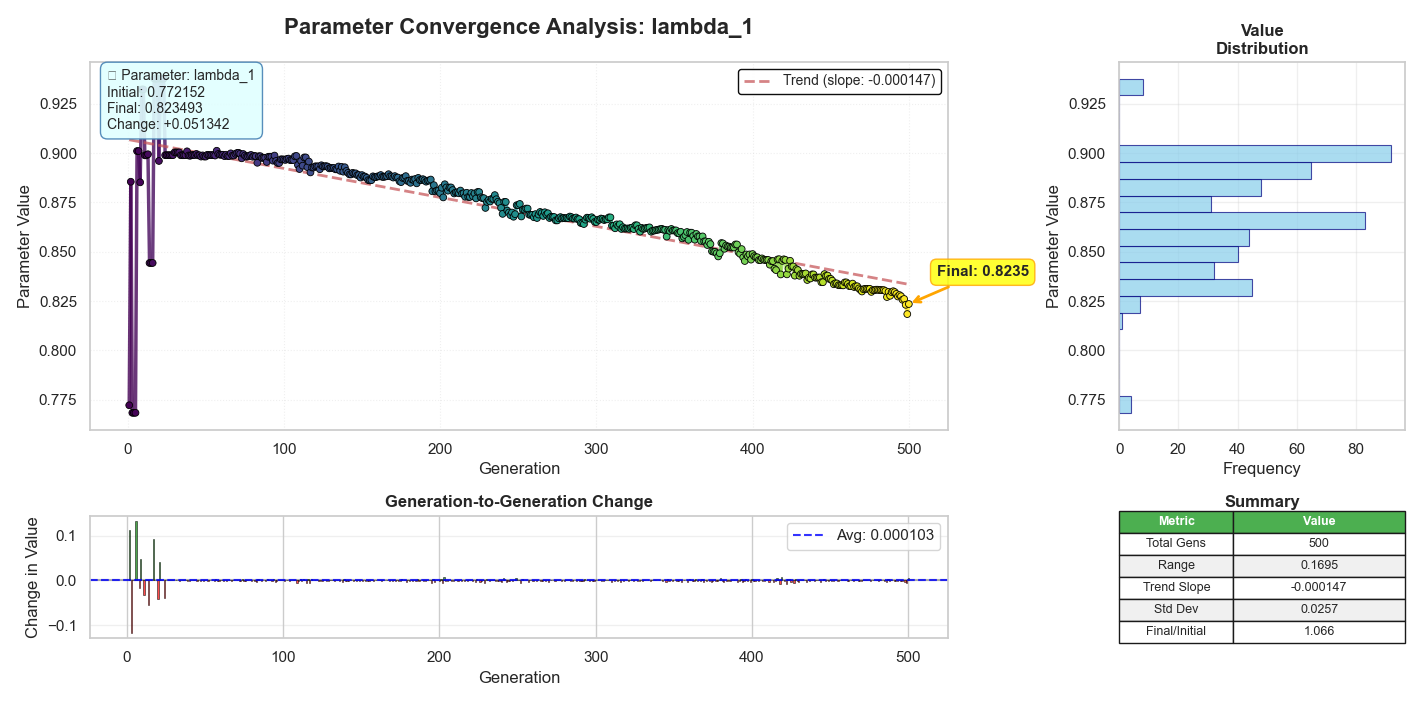
\includegraphics[width=\linewidth]{picture19.png}%
  \caption{همگراییِ پارامترهای \(\lambda\): (a) \(\lambda_1\).}
  \label{fig:lambda_convergence}
\end{figure}

\begin{figure}[h]\ContinuedFloat
  \centering
  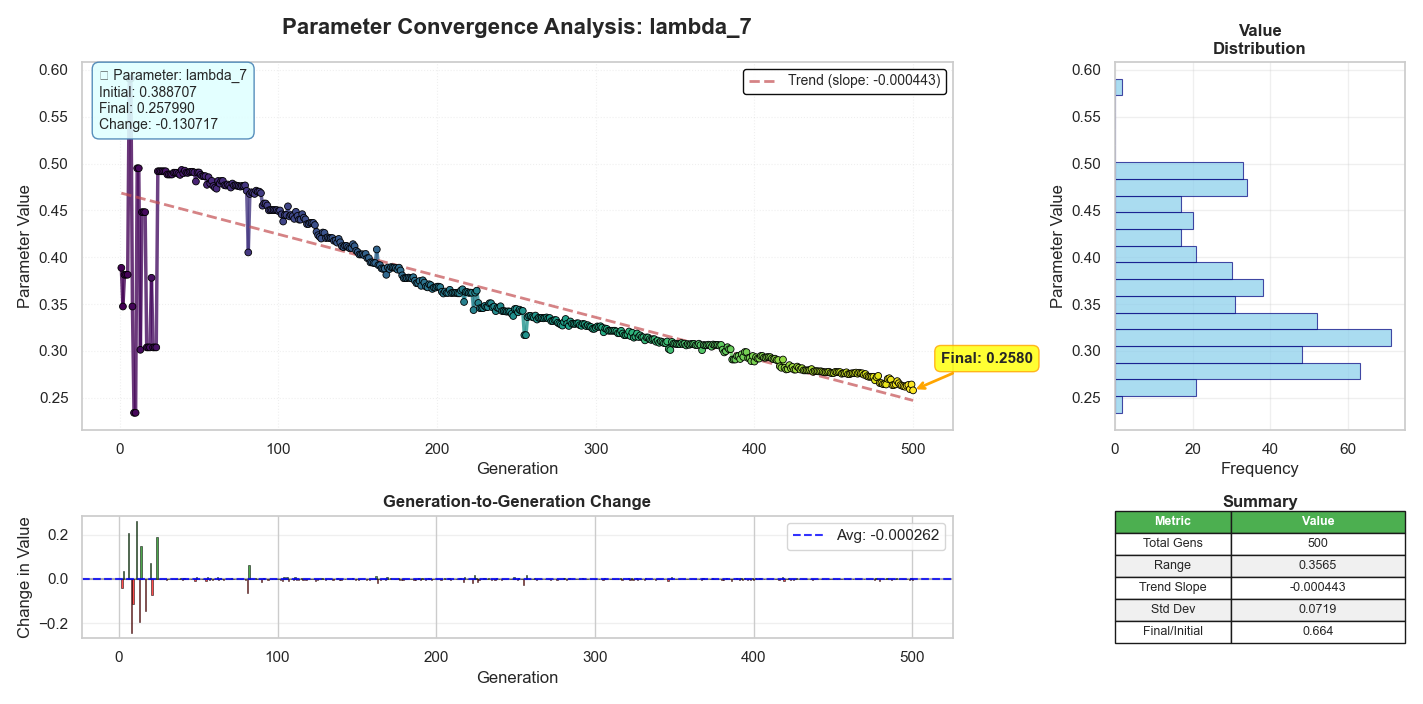
\includegraphics[width=\linewidth]{picture20.png}%
  \caption{(b) \(\lambda_7\).}
\end{figure}

\begin{figure}[h]\ContinuedFloat
  \centering
  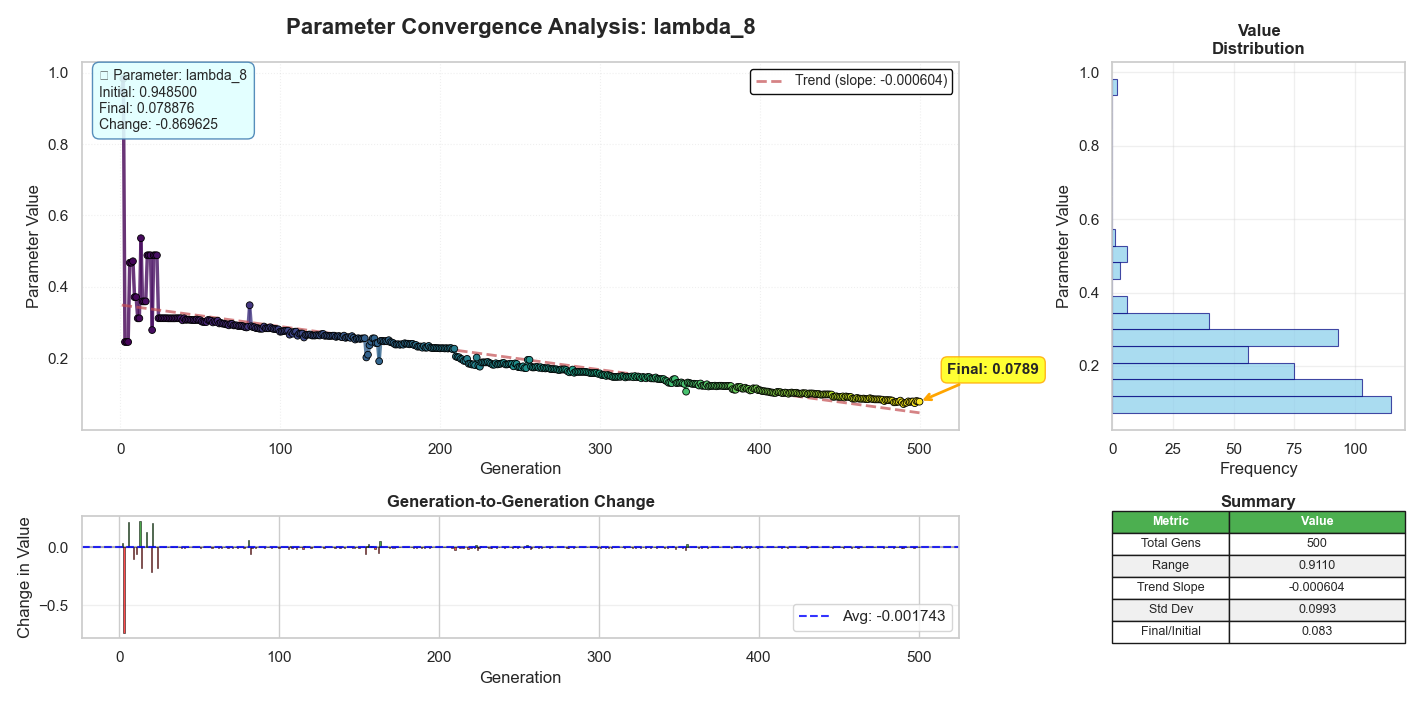
\includegraphics[width=\linewidth]{picture21.png}%
  \caption{(c) \(\lambda_8\).}
\end{figure}

\paragraph{تحلیل پارامترهای \(\lambda\) در شکل \ref{fig:lambda_convergence}}

\textbf{بخش (a) — \(\lambda_1\):}
در بخش (a) از شکل \ref{fig:lambda_convergence}، \(\lambda_1\) طی \(500\) نسل رهگیری شده است. مقدار آغازین \(\lambda_1=0.772152\) و مقدار نهایی \(\lambda_1=0.823493\) گزارش شده است؛ افزایش خالص برابر با \(0.051342\) است. روند خطی برازش‌شده شیب \(-1.47\times 10^{-4}\) به ازای هر نسل دارد، در حالی که میانگین تغییر نسل‌به‌نسل \(+1.03\times 10^{-4}\) اندازه‌گیری شده است. بازه مشاهده‌شده \(0.1695\) و انحراف معیار \(0.0257\) است. توزیع مقادیر عمدتا بین \(0.84\) تا \(0.90\) متمرکز است. پس از یک تنظیم کوتاه اولیه، مسیر آرام و کم‌نوسانی دنبال شده و درون ناحیه مجاز مستقر می‌شود. مقدار نهاییِ درونی نشان می‌دهد \(\lambda_1\) به عنوان یک متغیر تنظیم فعال باقی مانده است.

\medskip
\textbf{بخش (b) — \(\lambda_7\):}
در بخش (b) از شکل \ref{fig:lambda_convergence}، \(\lambda_7\) از \(0.388707\) به \(0.257990\) کاهش یافته است؛ کاهش خالص برابر با \(0.130717\). شیب روند خطی برازش‌شده \(-4.43\times 10^{-4}\) به ازای هر نسل و میانگین تغییر نسل‌به‌نسل \(-2.62\times 10^{-4}\) گزارش شده است. گستره در طول اجرا \(0.3565\) و انحراف معیار \(0.0719\) است. یک رانش نزولی پیوسته با کوچک شدن تدریجی گام‌ها مشاهده می‌شود. مقدار نهایی نشان می‌دهد \(\lambda_7\) در کارایی \lr{DVA} نقش داشته است.

\medskip
\textbf{بخش (c) — \(\lambda_8\):}
در بخش (c) از شکل \ref{fig:lambda_convergence}، \(\lambda_8\) طی \(500\) نسل پایش شده است. مقدار آن از \(0.948500\) به \(0.078876\) رسیده است؛ تغییر خالص \(-0.869625\). شیب روند خطی \(-6.04\times 10^{-4}\) به ازای هر نسل و میانگین تغییر نسل‌به‌نسل \(-1.743\times 10^{-3}\) است. بازه مشاهده‌شده \(0.9110\) و انحراف معیار \(0.0993\) گزارش شده‌اند. توزیع مقادیر در نسل‌های پایانی جرم قابل توجهی نزدیک به مقادیر کوچک نشان می‌دهد. یک افت سریع به سمت کران پایین بازه کاوش‌شده مشاهده می‌شود و پس از آن تنها اصلاحات جزئی رخ می‌دهد. مقدار نهایی کوچک دلالت دارد که \(\lambda_8\) عملا توسط فرایند بهینه‌سازی کم‌اهمیت شده است؛ همسو با هدف تنکی و پرهیز از اثرگذاری تنظیمی غیرضروری.



% ===== Fig. 10: Convergence of nu parameters (a)(b)(c), vertically stacked =====
\begin{figure}[h]
  \centering
  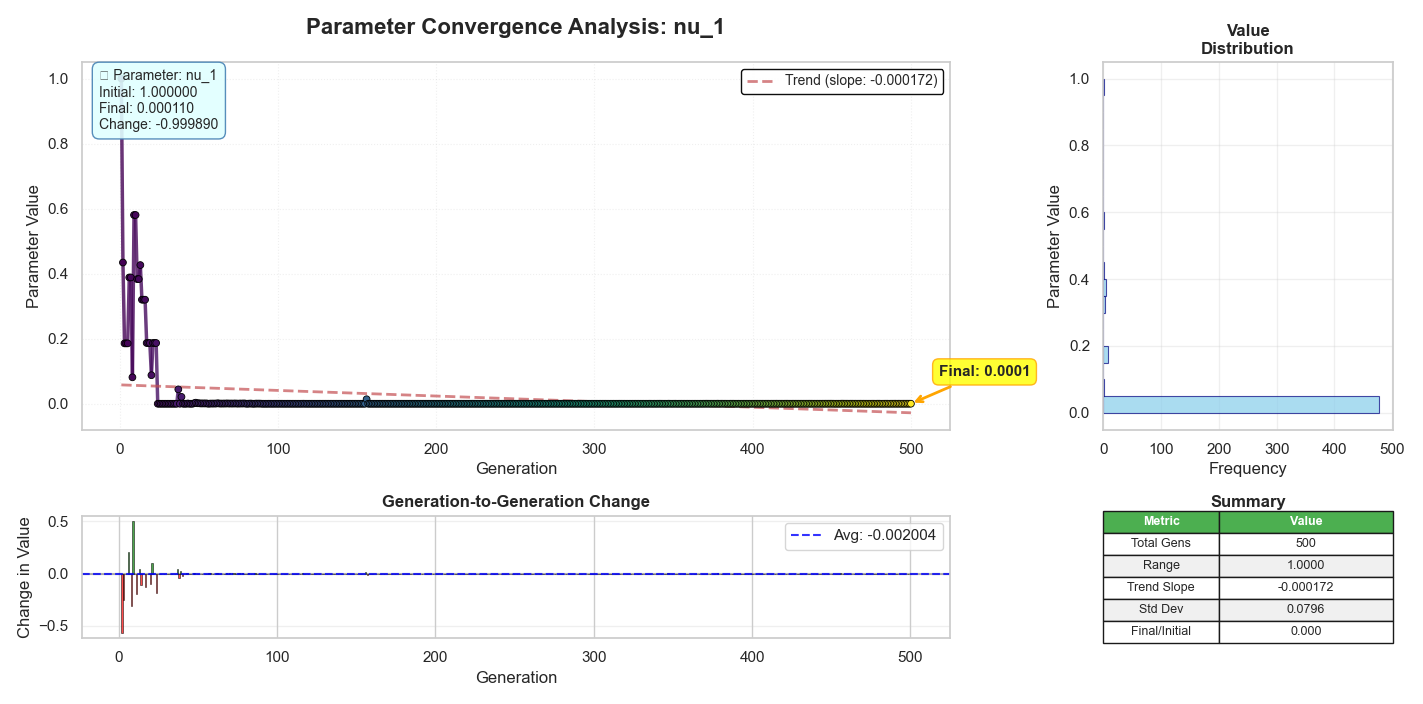
\includegraphics[width=\linewidth]{picture22.png}%
  \caption{همگراییِ پارامترهای \(\nu\): (a) \(\nu_1\).}
  \label{fig:nu_convergence}
\end{figure}

\begin{figure}[h]\ContinuedFloat
  \centering
  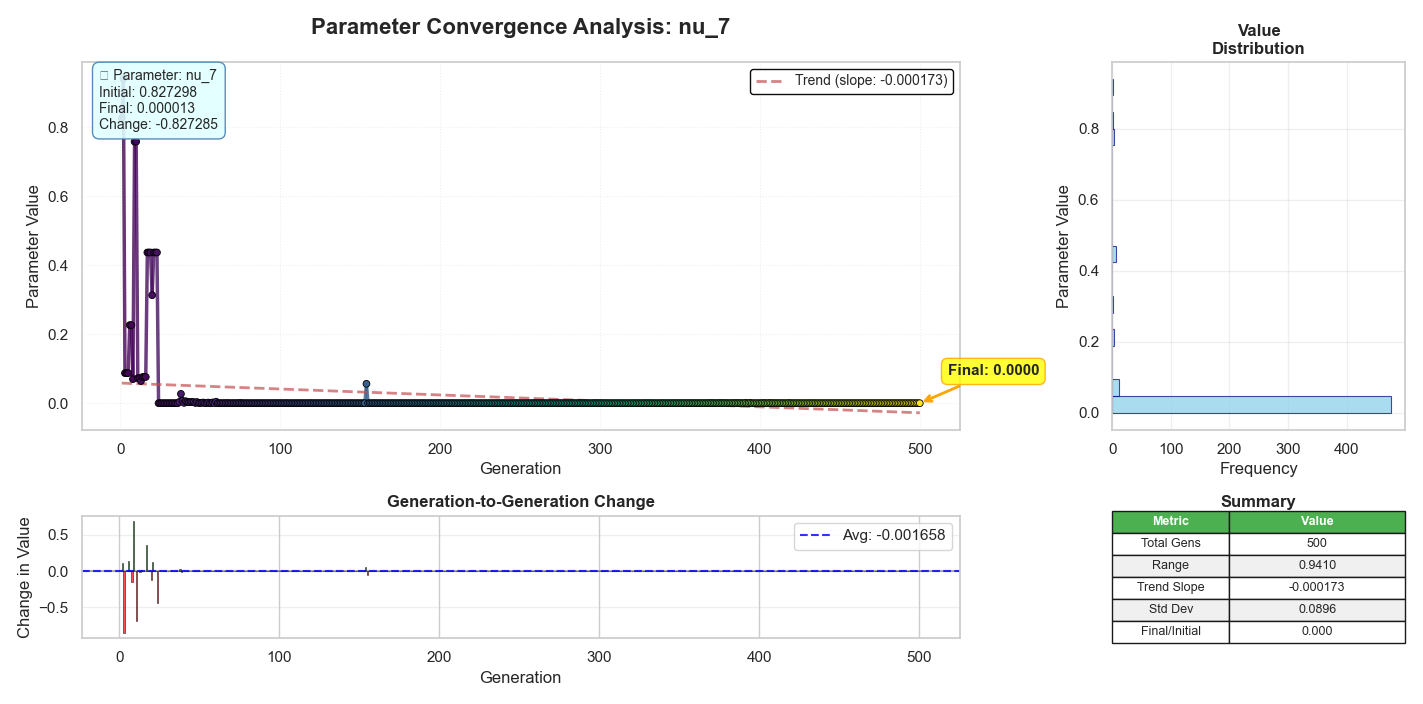
\includegraphics[width=\linewidth]{picture23.png}%
  \caption{(b) \(\nu_7\).}
\end{figure}

\begin{figure}[h]\ContinuedFloat
  \centering
  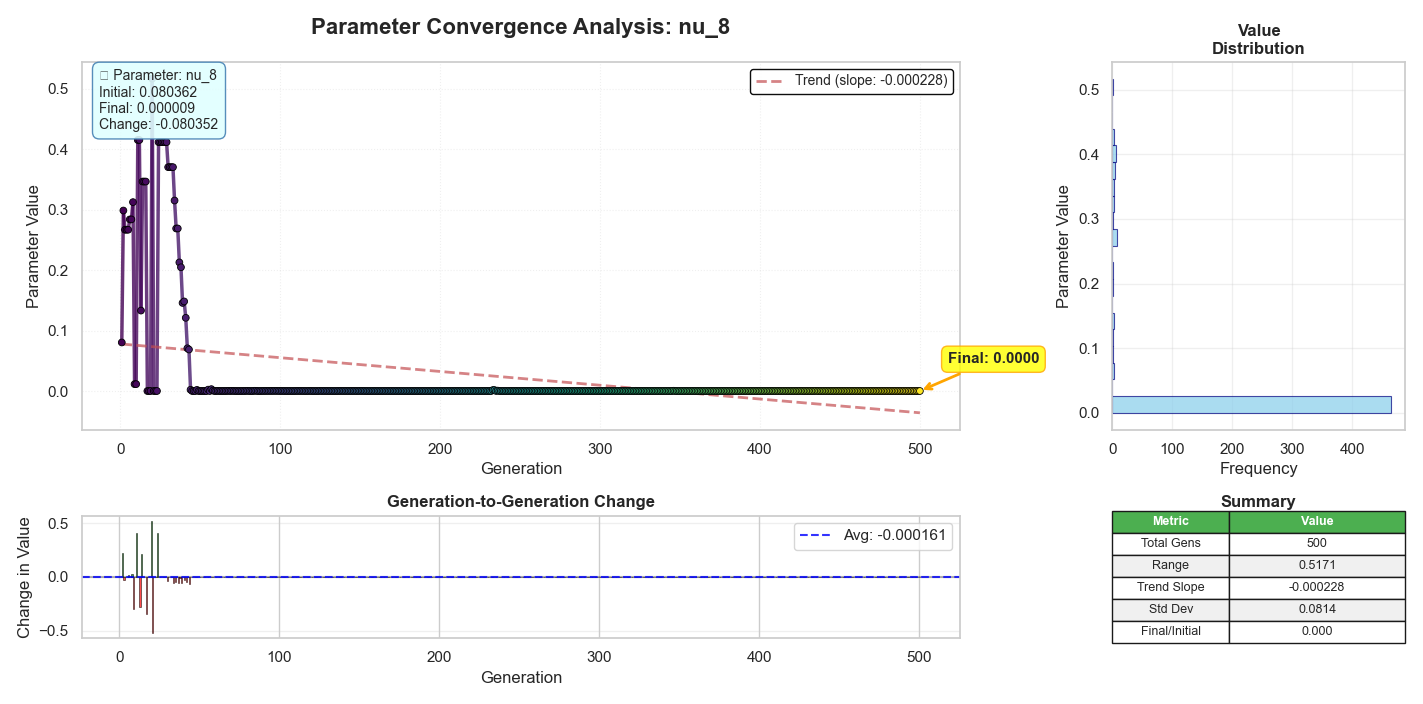
\includegraphics[width=\linewidth]{picture24.png}%
  \caption{(c) \(\nu_8\).}
\end{figure}

\paragraph{تحليل پارامترهاي $\nu$ در شكل‌هاي \ref{fig:nu_convergence}(a)–(c)}
در شكل‌هاي \ref{fig:nu_convergence}(a)، \ref{fig:nu_convergence}(b) و \ref{fig:nu_convergence}(c)، همگراييِ $\nu_1$، $\nu_7$ و $\nu_8$ در بازه‌اي به طول $500$ نسل گزارش شده است. مقادير آغازين به‌ترتيب $1.000000$، $0.827298$ و $0.080362$ ثبت شده و مقادير نهاييِ متناظر $0.000110$، $0.000013$ و $0.000009$ به‌دست آمده است؛ كاهشِ خالص به‌ترتيب $0.999890$، $0.827285$ و $0.080353$ مي‌باشد. گستره‌هاي مشاهده‌شده براي $\nu_1$، $\nu_7$ و $\nu_8$ به‌ترتيب $1.0000$، $0.9410$ و $0.5171$ و انحراف‌معيارها $0.0796$، $0.0896$ و $0.0814$ گزارش شده است. خطوطِ روندِ خطي با شيب‌هاي $-1.72\times 10^{-4}$، $-1.73\times 10^{-4}$ و $-2.28\times 10^{-4}$ به‌ازاي هر نسل برازش داده شده‌اند و ميانگينِ تغييراتِ نسل‌به‌نسل به‌ترتيب $-2.004\times 10^{-3}$، $-1.658\times 10^{-3}$ و $-1.61\times 10^{-4}$ اندازه‌گيري شده است. در هر پنل، پله‌هاي نزوليِ بزرگ در ابتداي اجرا در نمودارِ افزايش‌ها ديده مي‌شود و در ادامه تغييرات در نزديكيِ صفر خوشه‌بندي مي‌شوند. هيستوگرامِ مقادير عمدتاً در كمترينِ بين متمركز است و سكوي‌هاي طولانيِ نزديك به صفر در مسيرها مشاهده مي‌شود. در مجموع، اين الگوها نشان مي‌دهند كه پارامترهاي $\nu$ به‌صورت منسجم به سمتِ بي‌اثري رانده شده و عملاً توسط بهينه‌سازي هرس شده‌اند؛ اين رفتار با هدفِ تنكي و كاهشِ تعدادِ پارامترهايِ فعال \lr{DVA} سازگار است. خلاصه‌ي همگراييِ پارامتر-به-پارامتر در جدول~\ref{tab:conv_summary} ارائه شده است.



\begin{table}[htbp]
\centering
\caption{خلاصه همگراییِ همه پارامترهای تنظیم‌شده در \(500\) نسل}
\label{tab:conv_summary}
\scriptsize
\setlength{\tabcolsep}{3.5pt}
\renewcommand{\arraystretch}{1.25}
\begin{tabular}{c c c c c c c c p{0.38\textwidth}}
\toprule
\textbf{پارامتر} & \textbf{آغازین} & \textbf{نهایی} & $\Delta$ & \textbf{شیبِ روند} & \textbf{میانگین \(\Delta\)/نسل} & \textbf{گستره} & \lr{SD} & \textbf{نتیجه همگرایی} \\
\midrule
\(\beta_1\) & $0.029003$ & $0.015239$ & $-0.013764$ & $-6.0\times 10^{-6}$ & $-2.8\times 10^{-5}$ & $0.0307$ & $0.0028$ & پایدار درونی؛ به‌عنوان تنظیم‌گرِ کوچکِ فعال باقی ماند \\
\(\beta_7\) & $0.591281$ & $0.550909$ & $-0.040372$ & $-4.75\times 10^{-4}$ & $-8.1\times 10^{-5}$ & $0.3503$ & $0.0712$ & پایدار درونی؛ نقشِ غالب در پاسخ \\
\(\beta_8\) & $0.771658$ & $0.000106$ & $-0.771553$ & $-2.93\times 10^{-4}$ & $-1.546\times 10^{-3}$ & $0.7717$ & $0.0621$ & نزدیکِ صفر رانده شد؛ عملاً هرس شد \\
\(\lambda_1\) & $0.772152$ & $0.823493$ & $+0.051342$ & $-1.47\times 10^{-4}$ & $+1.03\times 10^{-4}$ & $0.1695$ & $0.0257$ & پایدار درونی؛ پارامترِ فعال باقی ماند \\
\(\lambda_7\) & $0.388707$ & $0.257990$ & $-0.130717$ & $-4.43\times 10^{-4}$ & $-2.62\times 10^{-4}$ & $0.3565$ & $0.0719$ & پایدار درونی؛ بدونِ رسیدن به کران‌ها مؤثر بود \\
\(\lambda_8\) & $0.948500$ & $0.078876$ & $-0.869625$ & $-6.04\times 10^{-4}$ & $-1.743\times 10^{-3}$ & $0.9110$ & $0.0993$ & به مقدارِ کوچک کاهش یافت؛ اثرگذاری کم‌وزن شد \\
\(\mu_1\) & $0.393887$ & $0.367100$ & $-0.026756$ & $-3.41\times 10^{-4}$ & $-5.4\times 10^{-5}$ & $0.2159$ & $0.0535$ & کاهشِ تدریجی و پایدارسازیِ درونی \\
\(\nu_1\) & $1.000000$ & $0.000110$ & $-0.999890$ & $-1.72\times 10^{-4}$ & $-2.004\times 10^{-3}$ & $1.0000$ & $0.0796$ & فروپاشی به صفر؛ هرس‌شده توسط تنکی \\
\(\nu_7\) & $0.827298$ & $0.000013$ & $-0.827285$ & $-1.73\times 10^{-4}$ & $-1.658\times 10^{-3}$ & $0.9410$ & $0.0896$ & فروپاشی به صفر؛ هرس‌شده توسط تنکی \\
\(\nu_8\) & $0.080362$ & $0.000009$ & $-0.080353$ & $-2.28\times 10^{-4}$ & $-1.61\times 10^{-4}$ & $0.5171$ & $0.0814$ & فروپاشی به صفر؛ هرس‌شده توسط تنکی \\
\bottomrule
\end{tabular}
\end{table}

\section{جمع‌بندي}

\noindent براي دگرگون كردن پاسخ سازه ميزبان در \lr{FRF}، \lr{DVA}‌ها ادوات پسيـوي‌اند كه به سازه ميزبان متصل مي‌شوند. كارايي آن‌ها به چيدمان و تنظيم جرم‌ها، فنرها، ميراگرها و \lr{inerter}‌ها وابسته است؛ تركيبي كه فضاي طراحي پرابعاد و غالباً نا‌محدب پديد مي‌آورد. در رويه‌هاي مرسوم، يك شكاف شناسايي شد: معيار تك‌مقياسيِ قابل تنظيم براي ديكته كردن شكل \lr{FRF} وجود نداشت؛ از تعيينِ جايگاه قله‌ها و پهناي باندِ اجتناب گرفته تا دامنه قله‌ها و شاخص‌هاي مشابه. نتيجه آن بود كه طراحي‌ها بيش از نياز، از مؤلفه‌ها و متغيرهاي تنظيم بهره مي‌گرفتند؛ چرا كه چارچوب‌هاي بهينه‌سازي به ندرت از پيچيدگي غيرضروري مي‌كاستند.

\noindent براي رفع اين نياز، هدف اصلي تعريف يك مقياس امتيازي واحد به نام \emph{معيار تكين} \(C_s\) بود. در ساخت اين مقياس، سنجه‌هاي عملكرد ابتدا نرمال مي‌شوند و سپس با وزن‌هايي كه مستقيماً توسط كاربر انتخاب مي‌گردند تركيب مي‌شوند. امتياز برازندگي از سه جزء تشكيل مي‌شود: جزء انحرافِ \(C_s\) كه \lr{FRF} را به سمت اهداف اعلام‌شده مي‌كشاند؛ جزء خطاي هدف كه ميزان نزديكي پاسخِ حاصل به اهداف را مي‌سنجد؛ و جريمه تنكي كه پارامترهاي غيرضروري را مي‌كاهد و طرح‌هاي ساده را ترجيح مي‌دهد.

\noindent سپس از يك \lr{GA} براي جست‌وجوي فضاي طراحي و يافتن راه‌حل بهينه براي تابع برازندگي استفاده شد. مدل‌سازي، تحليل \lr{FRF}، بهينه‌سازي و پس‌پردازش تا سقف پنج درجه آزادي در نرم‌افزار \lr{DeVana} (توسعه دهي نويسندگان) يكپارچه شد و كل جريان كار با آن پياده‌سازي گرديد. روش‌شناسي با يك بنچمارك كاملاً كوپل \lr{1DOF–1DOF} ارزيابي شد؛ در اين بنچمارك، سامانه اصلي و جذب‌كننده هر دو به دو پايه متحرك از طريق فنر، ميراگر و \lr{inerter} متصل بودند. بازه \(1000\)\,\lr{Hz} تا \(2000\)\,\lr{Hz} به عنوان باندِ اجتناب تعيين شد؛ پاسخِ درون باند توسط \lr{DVA} بهينه سركوب گرديد و دو قله باريك در نزديكي لبه‌هاي باند شكل گرفت. پاسخِ خارج از باند نزديك به خط مبنا باقي ماند. تاريخچه‌هاي برازندگي بهبود سريع ابتدايي را نشان دادند و سپس در مقاديري نزديك به تلرانس همگرايي پايدار شدند. با تفكيك برازندگي به مؤلفه‌ها، روشن شد كنترل جايگاه قله و پهناي باند محقق شده و جزء تنكي مانع تنظيم‌هاي زائد گرديده است. تحليل همگراييِ تك‌تك پارامترها نشان داد تنها زيرمجموعه‌اي كوچك در نقطه بهينه فعال باقي مي‌ماند: همه پارامترهاي \(\nu\) به مقادير نزديك صفر رسيدند و عملاً هرس شدند؛ \(\beta_1\)، \(\beta_7\)، \(\mu_1\)، \(\lambda_1\) و \(\lambda_7\) در نقاط دروني پايدار شدند كه نشانگر وجود بهينه قابل شناسايي (نه رفتارِ محدودشده به مرز) است؛ و \(\beta_8\) و \(\lambda_8\) به مقادير كوچك فروكاستند كه با هدف جلوگيري از استفاده بيش از حد از مؤلفه‌هاي جذب‌كننده سازگار است.

\noindent پيامدهاي كاربردي چندي از اين چارچوب حاصل مي‌شود. نخست، \(C_s\) روشي مستقيم و قابل تفسير براي كُدگذاري نيتِ طراحي فراهم مي‌كند: اهدافِ مربوط به دامنه قله‌ها، جايگاه قله‌ها و پهناي باند را مي‌توان به‌صراحت بيان كرد و بهينه‌ساز آن‌ها را برآورده مي‌كند. دوم، گنجاندن تنكي در تابع هدف به راه‌حل‌هاي كم‌پيچيدگي مي‌انجامد؛ امري كه جرم، هزينه و نگهداشت را كاهش مي‌دهد و حساسيت نسبت به \lr{detuning} و تولرانس‌هاي ساخت را كم مي‌كند. سوم، \lr{GA} بدون بازتنظيمِ دستيِ پارامترهاي الگوريتمي همگراييِ پايدار ارائه داد و به كارگيري در سامانه‌هاي جديد را ساده كرد. چهارم، پياده‌سازي در \lr{DeVana} مسير تكرارپذيري از تعريفِ مدل تا مشخصات سخت‌افزاريِ تنظيم‌شده فراهم مي‌كند و امكان مطالعه‌هاي \lr{what-if} سريع را در خانواده‌هاي جذب‌كننده — از جمله چيدمان‌هاي تقويت‌شده با \lr{inerter} — ميسر مي‌سازد.

\noindent در جمع‌بندي، چارچوبي يكپارچه براي طراحي \lr{DVA} ارائه شد كه معيارِ تكينِ قابل تنظيم و نرمال‌شده را با يك \lr{GA} تطبيقي در محيط \lr{DeVana} تركيب مي‌كند. اين رويكرد، شكل‌دهي مستقيم \lr{FRF} را ممكن مي‌سازد و هم‌زمان از افراط در تعداد پارامترهاي جذب‌كننده جلوگيري مي‌كند. مطالعه بنچمارك نشان داد كه باندِ اجتنابِ مشخص قابل حفاظت است و طرح نهايي تنك و قابل تفسير باقي مي‌ماند. اين نتايج پايه‌اي عملي براي طراحيِ كارآمدِ جذب‌كننده‌هاي هدف‌محور فراهم مي‌كند و مسير روشني به سمت راه‌حل‌هاي مقاوم، بلادرنگ و قابل راستي‌آزماييِ تجربي مي‌گشايد.






%-- فصل پنجم


\chapter{معرفی نرم‌افزار نوآورانه \lr{DeVana}}

\section{چالش عدم تکرارپذیری نتایج بهینه‌سازی}

در فرآیند بهینه‌سازی پارامترهای جاذب‌های دینامیکی ارتعاشات (\lr{Dynamic Vibration Absorbers - DVAs})، یکی از چالش‌های اساسی که طراحان با آن مواجه هستند، عدم تکرارپذیری نتایج است. به عبارت دیگر، فارغ از روش بهینه‌سازی انتخاب شده و اجرای موفق فرآیند بهینه‌سازی، مجموعه پارامترهای بهینه به دست آمده در هر اجرا متفاوت است و نمی‌توان به یک جواب منحصر به فرد دست یافت.

این مسئله نه تنها ناشی از ماهیت تصادفی الگوریتم‌های بهینه‌سازی است، بلکه ریشه در پیچیدگی فضای طراحی، وجود چندین مینیمم محلی، و تأثیر پارامترهای مختلف سیستم دارد. در شرایط عملیاتی واقعی، این عدم قطعیت می‌تواند منجر به تصمیم‌گیری‌های نادرست شود و نیاز به رویکردی جامع‌تر برای تحلیل و اعتبارسنجی نتایج دارد.

\section{نیاز به مفهوم «زمین بازی» برای طراحان}

چالش عدم تکرارپذیری نتایج، ضرورت وجود یک محیط انعطاف‌پذیر را برای طراحان برجسته می‌کند که بتوانند آزادانه در فضای طراحی حرکت کنند و از روش‌های مختلف تحلیل استفاده نمایند. این مفهوم که ما آن را «زمین بازی» می‌نامیم، به طراحان اجازه می‌دهد تا:

\begin{enumerate}
\item روش‌های بهینه‌سازی مختلف را با تنظیمات متفاوت مقایسه کنند
\item تحلیل آماری بر روی نتایج چند اجرای مختلف انجام دهند
\item فضای طراحی را تغییر داده و تأثیر آن را بررسی کنند
\item روش‌های تحلیل حساسیت را برای درک بهتر روابط بین پارامترها اعمال کنند
\item تصمیم‌گیری آگاهانه بر اساس مجموعه کاملی از تحلیل‌ها انجام دهند
\end{enumerate}

این رویکرد نه تنها به حل مسئله عدم تکرارپذیری کمک می‌کند، بلکه قدرت تصمیم‌گیری طراحان را در شرایط پیچیده عملیاتی افزایش می‌دهد.

\section{معرفی \lr{DeVana}: اولین نرم‌افزار از نوع خود}

برای پاسخ به این نیازها، نرم‌افزار نوآورانه \lr{DeVana} توسط نویسندگان این پایان‌نامه توسعه یافته است. \lr{DeVana} اولین نرم‌افزار از نوع خود در جهان است که به صورت متن‌باز ارائه شده و محیط کاملی برای طراحی و بهینه‌سازی جاذب‌های دینامیکی ارتعاشات فراهم می‌آورد.

این نرم‌افزار با رویکردی جامع، تمامی روش‌های توسعه‌یافته در این پژوهش را پیاده‌سازی کرده و زمین بازی نهایی برای طراحان محسوب می‌شود. \lr{DeVana} نه تنها امکان اجرای الگوریتم‌های بهینه‌سازی پیشرفته را فراهم می‌آورد، بلکه ابزارهای متنوعی برای تحلیل و مقایسه نتایج در اختیار طراحان قرار می‌دهد.

\section{قابلیت‌های بهینه‌سازی در \lr{DeVana}}

\lr{DeVana} مجموعه کاملی از الگوریتم‌های بهینه‌سازی پیشرفته را ارائه می‌دهد که هر کدام با ویژگی‌های منحصر به فرد خود، پاسخگوی نیازهای مختلف طراحان هستند:

\subsection{الگوریتم ژنتیک (\lr{Genetic Algorithm - GA})}

این الگوریتم که پایه بسیاری از روش‌های بهینه‌سازی هوشمند است، با قابلیت کنترل تطبیقی پارامترها ارائه شده است. طراحان می‌توانند نرخ جهش، اندازه جمعیت، و استراتژی انتخاب را به صورت دینامیکی تنظیم کنند تا بهترین عملکرد را در فضای طراحی پیچیده به دست آورند.

\subsection{بهینه‌سازی ازدحام ذرات (\lr{Particle Swarm Optimization - PSO})}

روش \lr{PSO} با قابلیت پشتیبانی از توپولوژی‌های مختلف (حلقه‌ای، ستاره‌ای، و تصادفی) پیاده‌سازی شده است. این روش امکان تنظیم پارامترهای یادگیری اجتماعی و فردی را فراهم می‌آورد و برای مسائل با فضای جستجوی پیوسته بسیار کارآمد است.

\subsection{تفاوت‌گیری (\lr{Differential Evolution - DE})}

الگوریتم \lr{DE} با استراتژی‌های مختلف جهش و ترکیب، امکان کاوش کارآمد فضای طراحی را فراهم می‌آورد. این روش به ویژه برای مسائل با محدودیت‌های غیرخطی مناسب است و قابلیت تنظیم پارامترهای جهش و متقاطع را ارائه می‌دهد.

\subsection{شبیه‌سازی آنیلینگ (\lr{Simulated Annealing - SA})}

روش \lr{SA} با قابلیت کنترل دینامیکی دما و استراتژی‌های پذیرشی مختلف، امکان فرار از مینیمم‌های محلی را فراهم می‌آورد. این روش برای مسائل ترکیبی و پیوسته کاربرد دارد.

\subsection{استراتژی‌های تکاملی (\lr{Covariance Matrix Adaptation Evolution Strategy - CMA-ES})}

این روش پیشرفته با قابلیت تطبیق ماتریس کوواریانس، امکان مدل‌سازی توزیع احتمالاتی فضای جستجو را فراهم می‌آورد و برای مسائل با وابستگی پیچیده بین پارامترها بسیار کارآمد است.

\subsection{یادگیری تقویتی (\lr{Reinforcement Learning - RL})}

روش \lr{RL} با قابلیت یادگیری از تعامل با محیط، امکان توسعه استراتژی‌های بهینه‌سازی تطبیقی را فراهم می‌آورد که می‌تواند با شرایط مسئله سازگار شود.

\section{قابلیت‌های تحلیل حساسیت}

\lr{DeVana} ابزارهای پیشرفته‌ای برای تحلیل حساسیت ارائه می‌دهد که به طراحان کمک می‌کنند تا تأثیر هر پارامتر بر عملکرد سیستم را درک کنند:

\subsection{تحلیل حساسیت سوبول (\lr{Sobol Sensitivity Analysis})}

این روش امکان محاسبه شاخص‌های حساسیت کلی و جزئی را فراهم می‌آورد و به طراحان کمک می‌کند تا پارامترهای کلیدی که بیشترین تأثیر را بر عملکرد سیستم دارند، شناسایی کنند.

\subsection{تحلیل حساسیت امگا (\lr{Omega Sensitivity Analysis})}

روش \lr{امگا} با قابلیت تحلیل حساسیت بر حسب دامنه تغییرات پارامترها، امکان ارزیابی تأثیر نسبی هر پارامتر را در شرایط عملیاتی مختلف فراهم می‌آورد.

\section{قابلیت‌های تحلیل آماری}

یکی از ویژگی‌های منحصر به فرد \lr{DeVana}، قابلیت انجام تحلیل آماری بر روی نتایج چند اجرای مختلف است:

\subsection{آمار توصیفی نتایج}

نرم‌افزار امکان محاسبه میانگین، واریانس، و سایر آمار توصیفی برای مجموعه نتایج چند اجرا را فراهم می‌آورد.

\subsection{تحلیل توزیع احتمالاتی}

با استفاده از تکنیک‌های آماری پیشرفته، طراحان می‌توانند توزیع احتمالاتی پارامترهای بهینه را تحلیل کرده و اطمینان‌پذیری نتایج را ارزیابی کنند.

\subsection{مقایسه روش‌های مختلف}

\lr{DeVana} امکان مقایسه آماری عملکرد روش‌های بهینه‌سازی مختلف را فراهم می‌آورد و به طراحان کمک می‌کند تا بهترین روش را برای مسئله خاص خود انتخاب کنند.

\section{ساختار نرم‌افزاری \lr{DeVana}}

\subsection{معماری کلی}

نرم‌افزار \lr{DeVana} با معماری ماژولار و انعطاف‌پذیر طراحی شده است که امکان توسعه و افزودن قابلیت‌های جدید را فراهم می‌آورد. ساختار اصلی نرم‌افزار شامل بخش‌های زیر است:

\subsection{شاخص‌بندی ساختار نرم‌افزار}

\begin{figure}[H]
\centering
\begin{tikzpicture}[
    level 1/.style={sibling distance=4.2cm, level distance=2.0cm},
    level 2/.style={sibling distance=3.0cm, level distance=1.6cm},
    level 3/.style={sibling distance=2.2cm, level distance=1.3cm},
    every node/.style={
        draw,
        rectangle,
        rounded corners=3pt,
        text width=3.2cm,
        minimum height=0.9cm,
        inner sep=3pt,
        align=center,
        font=\footnotesize
    },
    root/.style={
        fill=blue!20,
        font=\small\bfseries
    },
    main/.style={
        fill=green!20,
        font=\footnotesize
    },
    worker/.style={
        fill=orange!20,
        font=\footnotesize
    }
]

% Root
\node[root] {\lr{codes/}}
    child {
        node[main] {\lr{run.py}\\فایل اصلی اجرا}
    }
    child {
        node[main] {\lr{mainwindow.py}\\پنجره اصلی}
    }
    child {
        node[main] {\lr{app\_info.py}\\اطلاعات برنامه}
    }
    child {
        node[main] {\lr{computational\_}\\\lr{metrics\_new.py}\\متریک‌های محاسباتی}
    }
    child {
        node[worker] {\lr{workers/}}
        child {
            node[worker] {\lr{GAWorker.py}\\الگوریتم ژنتیک}
        }
        child {
            node[worker] {\lr{PSOWorker.py}\\ازدحام ذرات}
        }
        child {
            node[worker] {\lr{DEWorker.py}\\تفاوت‌گیری}
        }
        child {
            node[worker] {\lr{SAWorker.py}\\شبیه‌سازی تبرید}
        }
        child {
            node[worker] {\lr{CMAESWorker.py}\\استراتژی تکاملی}
        }
        child {
            node[worker] {\lr{SobolWorker.py}\\تحلیل سوبول}
        }
        child {
            node[worker] {\lr{FRFWorker.py}\\پاسخ فرکانسی}
        }
        child {
            node[worker] {\lr{MemorySeeder.py}\\مدیریت حافظه}
        }
        child {
            node[worker] {\lr{NeuralSeeder.py}\\بذردهی عصبی}
        }
    };

\end{tikzpicture}
\caption{ساختار اصلی نرم‌افزار \lr{DeVana} - بخش اول}
\end{figure}

\begin{figure}[H]
\centering
\begin{tikzpicture}[
    level 1/.style={sibling distance=4.0cm, level distance=2.0cm},
    level 2/.style={sibling distance=2.8cm, level distance=1.6cm},
    level 3/.style={sibling distance=2.0cm, level distance=1.3cm},
    every node/.style={
        draw,
        rectangle,
        rounded corners=3pt,
        text width=3.1cm,
        minimum height=0.9cm,
        inner sep=3pt,
        align=center,
        font=\footnotesize
    },
    gui/.style={
        fill=purple!20,
        font=\footnotesize
    }
]

% GUI Branch
\node[gui] {\lr{gui/}\\رابط کاربری}
    child {
        node[gui] {\lr{main\_window/}}
        child {
            node[gui] {\lr{ga\_mixin.py}\\رابط \lr{GA}}
        }
        child {
            node[gui] {\lr{pso\_mixin.py}\\رابط \lr{PSO}}
        }
        child {
            node[gui] {\lr{de\_mixin.py}\\رابط \lr{DE}}
        }
        child {
            node[gui] {\lr{sobol\_mixin.py}\\رابط سوبول}
        }
        child {
            node[gui] {\lr{omega\_sensitivity\_}\\\lr{mixin.py}\\حساسیت \lr{امگا}}
        }
        child {
            node[gui] {\lr{frf\_mixin.py}\\رابط \lr{FRF}}
        }
    }
    child {
        node[gui] {\lr{menu\_mixin.py}\\میکسین منو}
    }
    child {
        node[gui] {\lr{beam\_mixin.py}\\میکسین تیر}
    }
    child {
        node[gui] {\lr{widgets.py}\\ابزارک‌های سفارشی}
    };

\end{tikzpicture}
\caption{ساختار رابط کاربری نرم‌افزار \lr{DeVana}}
\end{figure}

\begin{figure}[H]
\centering
\begin{tikzpicture}[
    level 1/.style={sibling distance=4.2cm, level distance=2.0cm},
    level 2/.style={sibling distance=3.0cm, level distance=1.6cm},
    level 3/.style={sibling distance=2.2cm, level distance=1.3cm},
    every node/.style={
        draw,
        rectangle,
        rounded corners=3pt,
        text width=3.0cm,
        minimum height=0.9cm,
        inner sep=3pt,
        align=center,
        font=\footnotesize
    },
    module/.style={
        fill=yellow!20,
        font=\footnotesize
    },
    domainNode/.style={
        fill=red!20,
        font=\footnotesize
    }
]

% Modules and Domain
\node[module] {\lr{modules/}\\ماژول‌های کاربردی}
    child {
        node[module] {\lr{FRF.py}\\تحلیل پاسخ فرکانسی}
    }
    child {
        node[module] {\lr{sobol\_sensitivity.py}\\تحلیل حساسیت سوبول}
    };

\node[domainNode, below=2.0cm] {\lr{Continues\_beam/}\\تحلیل تیر پیوسته}
    child {
        node[domainNode] {\lr{beam/}}
        child {
            node[domainNode] {\lr{fem.py}\\عناصر محدود}
        }
        child {
            node[domainNode] {\lr{solver.py}\\حل‌کننده ارتعاشات}
        }
        child {
            node[domainNode] {\lr{properties.py}\\خواص مواد}
        }
    }
    child {
        node[domainNode] {\lr{ui/}\\رابط کاربری تیر}
    }
    child {
        node[domainNode] {\lr{utils.py}\\ابزارهای کمکی}
    };

\node[domainNode, below=4.0cm] {\lr{RL/}\\یادگیری تقویتی};
\node[module, below=5.0cm] {\lr{src/}\\منابع اضافی};

\end{tikzpicture}
\caption{ماژول‌های کاربردی و دامنه‌ای نرم‌افزار \lr{DeVana}}
\end{figure}

\begin{table}[H]
\centering
\caption{راهنمای رنگ‌بندی ساختار نرم‌افزار}
\begin{tabular}{|c|l|p{8cm}|}
\hline
\textbf{رنگ} & \textbf{نوع ماژول} & \textbf{توضیحات} \\
\hline
\cellcolor{blue!20} آبی & هسته اصلی & فایل‌های اصلی اجرا و مدیریت برنامه \\
\hline
\cellcolor{green!20} سبز & فایل‌های اجرایی & فایل‌های مسئول راه‌اندازی و کنترل کلی \\
\hline
\cellcolor{orange!20} نارنجی & کارگران & ماژول‌های پردازش موازی و الگوریتم‌ها \\
\hline
\cellcolor{purple!20} بنفش & رابط کاربری & اجزای مربوط به تعامل با کاربر \\
\hline
\cellcolor{yellow!20} زرد & ماژول‌های کاربردی & ابزارهای تحلیلی و محاسباتی \\
\hline
\cellcolor{red!20} قرمز & دامنه‌ای & ماژول‌های تخصصی و کاربردهای خاص \\
\hline
\end{tabular}
\end{table}
\subsection{توضیح ساختار}

\subsubsection{لایه اجرایی (\lr{Execution Layer})}

این لایه شامل فایل‌های اصلی \lr{run.py} و \lr{mainwindow.py} است که مسئولیت راه‌اندازی برنامه و مدیریت رابط کاربری اصلی را بر عهده دارند.

\subsubsection{لایه کارگران (\lr{Workers Layer})}

لایه \lr{workers} شامل کلاس‌های پردازش موازی است که هر کدام مسئول اجرای یک الگوریتم بهینه‌سازی یا تحلیل خاص هستند. این طراحی امکان اجرای همزمان چند روش را فراهم می‌آورد.

\subsubsection{لایه رابط کاربری (\lr{GUI Layer})}

لایه \lr{gui} با معماری میکسین، امکان ترکیب قابلیت‌های مختلف را فراهم می‌آورد. هر میکسین مسئول مدیریت یک جنبه خاص از رابط کاربری است.

\subsubsection{لایه کاربردی (\lr{Modules Layer})}

این لایه شامل ماژول‌های کاربردی مانند تحلیل پاسخ فرکانسی و تحلیل حساسیت است که توسط چندین قسمت برنامه استفاده می‌شوند.

\subsubsection{لایه دامنه (\lr{Domain Layer})}

لایه \lr{Continues\_beam} و \lr{RL} به ترتیب مسئول تحلیل تیرهای پیوسته و یادگیری تقویتی هستند و قابلیت‌های تخصصی نرم‌افزار را ارائه می‌دهند.

\section{نتیجه‌گیری}

نرم‌افزار \lr{DeVana} با ارائه محیطی جامع و انعطاف‌پذیر، پاسخ کاملی به چالش‌های طراحی جاذب‌های دینامیکی ارتعاشات ارائه می‌دهد. این نرم‌افزار نه تنها تمامی روش‌های توسعه‌یافته در این پژوهش را پیاده‌سازی کرده، بلکه با معماری ماژولار خود، امکان توسعه آینده و افزودن قابلیت‌های جدید را فراهم می‌آورد.

\lr{DeVana} به عنوان اولین نرم‌افزار از نوع خود، زمین بازی نهایی برای طراحان محسوب می‌شود که در آن می‌توانند آزادانه روش‌های مختلف را مقایسه کرده، تحلیل‌های متنوعی انجام دهند، و تصمیم‌گیری‌های آگاهانه‌تری اتخاذ کنند. این نرم‌افزار گامی بزرگ در جهت کاربردی‌سازی نتایج پژوهشی و تسهیل فرآیند طراحی در مهندسی مکانیک برمی‌دارد. 








%-- فصل نتیجه‌گیری
\chapter{نتیجه‌گیری و چشم‌اندازهای آینده}

\section{مرور کلی پژوهش و دستاوردهای اصلی}

پژوهش حاضر با رویکردی جامع و بین‌رشته‌ای به مسئله طراحی و بهینه‌سازی جاذب‌های دینامیکی ارتعاش پرداخته است. این پایان‌نامه فراتر از یک مطالعه فنی محدود، چارچوبی نوین برای حل چالش‌های طراحی \lr{DVA} در سیستم‌های پیچیده ارائه نموده که از روش‌شناسی علمی پیشرفته، تکنیک‌های عددی نوآورانه و ابزارهای نرم‌افزاری مدرن بهره می‌گیرد. رویکرد این پژوهش از شناسایی چالش‌های اساسی در طراحی \lr{DVA} آغاز شد و با یک مسیر سلسله‌مراتبی به توسعه راهکارهای جامع پرداخت. ابتدا محدودیت‌های روش‌های کلاسیک تحلیل و بهینه‌سازی مورد بررسی قرار گرفت، سپس معیارهای نوین ارزیابی عملکرد معرفی شد، الگوریتم‌های بهینه‌سازی پیشرفته توسعه یافت، نتایج در شرایط واقعی آزمایش و اعتبارسنجی شد و در نهایت ابزارهای نرم‌افزاری کاربردی پیاده‌سازی گردید.

این پژوهش نشان می‌دهد که با ترکیب رویکردهای علمی پیشرفته، روش‌های عددی کارآمد و ابزارهای نرم‌افزاری مدرن، می‌توان چالش‌های پیچیده مهندسی را به شیوه‌ای مؤثر و کارآمد حل نمود. نرم‌افزار \lr{DeVana} به‌عنوان یک دستاورد کلیدی، نه‌تنها ابزاری برای حل مسائل فعلی است، بلکه بستری برای نوآوری و توسعه آینده در حوزه طراحی \lr{DVA} فراهم می‌آورد.

\section{نوآوری‌های کلیدی و دستاوردهای علمی}

یکی از نوآوری‌های بنیادین این پژوهش، معرفی معیار \lr{Peak-Slope (PS)} به عنوان جایگزینی کارآمد برای معیارهای کلاسیک است. این معیار با سنجش شیب بین قله‌های پاسخ فرکانسی، ابزاری شهودی و ریاضیاتی برای ارزیابی عملکرد \lr{DVA} فراهم می‌آورد. مزیت اصلی این معیار در سادگی محاسباتی آن نهفته است که باعث کاهش پیچیدگی در مقایسه با معیار \lr{$H_\infty$} می‌شود. همچنین، قابلیت تفسیر فیزیکی این معیار امکان ارتباط مستقیم با مکانیسم جذب ارتعاش را فراهم می‌آورد و سازگاری آن با مدل‌سازی جانشین، امکان استفاده در چارچوب‌های پیشرفته را ممکن می‌سازد. این معیار برای سیستم‌های تک‌درجه و چنددرجه آزادی مناسب است و کاربرد گسترده‌ای در طراحی سیستم‌های ارتعاشی دارد.

نوآوری اصلی پژوهش در توسعه چارچوب \lr{Decoupled Peak-Slope (DPS)} نهفته است که با جداسازی پارامترهای طراحی، امکان بهینه‌سازی کارآمد را در فضای پارامتری پیچیده فراهم می‌آورد. چارچوب \lr{DPS} بر پایه اصول ریاضیاتی محکم استوار است و از تقریب خطی برای مدل‌سازی پاسخ \lr{PS} به صورت تابعی از پارامترها استفاده می‌کند. این رویکرد فضای چندبعدی را به مجموعه‌ای از مسائل تک‌متغیره تبدیل می‌کند و با استفاده از رگرسیون چندجمله‌ای درجه چهارم، دقت بالایی را تضمین می‌کند. مزیت اصلی این چارچوب در سرعت بالای محاسبات است که زمان بهینه‌سازی را تا ۹۰\% نسبت به روش‌های سنتی کاهش می‌دهد. همچنین، دقت قابل اطمینان این روش نتایج قطعی بدون وابستگی به شرایط اولیه فراهم می‌آورد و قابلیت تعمیم آن امکان اعمال در پیکربندی‌های مختلف سیستم را ممکن می‌سازد. سازگاری این چارچوب با کنترل پیشرفته نیز امکان توسعه به سامانه‌های نیمه‌فعال را فراهم می‌آورد.

علاوه بر این نوآوری‌ها، پژوهش حاضر کاتالوگ‌های طراحی تعمیم‌یافته را توسعه داده که امکان اعمال چارچوب \lr{DPS} در پیکربندی‌های مختلف سیستم را فراهم می‌آورد. این کاتالوگ‌ها با داشتن انعطاف‌پذیری ساختاری، سازگاری با تغییرات پارامترهای سیستم را ممکن می‌سازند و کتابخانه جامعی از شرایط عملیاتی مختلف را پوشش می‌دهند. قابلیت به‌روزرسانی آسان این کاتالوگ‌ها امکان گسترش با داده‌های جدید را فراهم می‌آورد و کارایی محاسباتی بالا نیاز به محاسبات تکراری را کاهش می‌دهد.

پژوهش حاضر همچنین با تحلیل آماری عدم قطعیت، به چالش عدم تکرارپذیری نتایج بهینه‌سازی پاسخ داده و روشی نوین برای مدیریت عدم قطعیت ارائه نموده است. این رویکرد از توزیع احتمالاتی برای مدل‌سازی نتایج، آمار توصیفی برای تحلیل میانگین و واریانس، و تست فرضیه برای ارزیابی معنی‌داری تفاوت‌ها استفاده می‌کند. همچنین، امکان پیش‌بینی اطمینان با تعیین محدوده‌های بهینه با سطح اطمینان مشخص فراهم می‌آورد.

\section{نرم‌افزار \lr{DeVana}: دستاوردی انقلابی در طراحی \lr{DVA}}

نرم‌افزار \lr{DeVana} که توسط نویسندگان این پژوهش توسعه یافته، یکی از دستاوردهای کلیدی و انقلابی این پایان‌نامه است. این نرم‌افزار به‌عنوان یک ابزار جامع و پیشرفته برای طراحی، تحلیل و بهینه‌سازی \lr{DVA} معرفی می‌شود که فراتر از یک ابزار محاسباتی ساده، بستری برای نوآوری در این حوزه فراهم می‌آورد. \lr{DeVana} با معماری ماژولار طراحی شده که امکان گسترش آسان و افزودن قابلیت‌های جدید را فراهم می‌آورد. این معماری شامل ماژول‌های مستقل برای جداسازی عملکردهای مختلف مانند مدلسازی، بهینه‌سازی و تحلیل است. رابط‌های برنامه‌نویسی پیشرفته امکان اتصال به سایر نرم‌افزارهای مهندسی را فراهم می‌آورد و سیستم پلاگین اجازه می‌دهد تا قابلیت‌های جدید بدون تغییر هسته اصلی اضافه شوند. پایگاه داده یکپارچه نیز امکان ذخیره و مدیریت کاتالوگ‌های طراحی را فراهم می‌آورد.

از نظر قابلیت‌های پیشرفته، \lr{DeVana} مجموعه کاملی از ابزارها را ارائه می‌دهد. این نرم‌افزار امکان شبیه‌سازی سیستم‌های پیچیده با عناصر پیشرفته مکانیکی مانند \lr{Inerter} را فراهم می‌آورد. الگوریتم‌های بهینه‌سازی متنوعی از روش‌های کلاسیک تا پیشرفته در این نرم‌افزار پیاده‌سازی شده‌اند. قابلیت تحلیل حساسیت امکان ارزیابی تأثیر پارامترها بر عملکرد سیستم را فراهم می‌آورد و ابزارهای بصری‌سازی پیشرفته نمایش گرافیکی نتایج و تحلیل‌ها را ممکن می‌سازند. همچنین، سیستم گزارش‌دهی هوشمند امکان تولید گزارش‌های فنی جامع و حرفه‌ای را فراهم می‌آورد.

یکی از ویژگی‌های منحصربه‌فرد \lr{DeVana}، انتشار به صورت کاملاً منبع‌باز است که اهمیت ویژه‌ای در توسعه علمی و فنی این حوزه دارد. این رویکرد منبع‌باز امکان دسترسی جهانی برای پژوهشگران و مهندسان در سراسر جهان را فراهم می‌آورد و شفافیت علمی کاملی را تضمین می‌کند. هر پژوهشگر می‌تواند کد منبع را بررسی و اعتبارسنجی کند، که این امر به افزایش اعتماد به نتایج و روش‌های به‌کار رفته کمک می‌کند. رویکرد منبع‌باز همچنین تسهیل‌کننده همکاری بین تیم‌های پژوهشی مختلف است و امکان توسعه پایدار توسط جامعه علمی را فراهم می‌آورد. علاوه بر این، \lr{DeVana} به‌عنوان یک منبع آموزشی ارزشمند برای دانشجویان و پژوهشگران عمل می‌کند که می‌توانند از طریق بررسی کد منبع، مفاهیم پیشرفته مهندسی را بیاموزند.

انتشار منبع‌باز \lr{DeVana} می‌تواند تأثیرات گسترده‌ای بر جامعه علمی داشته باشد. مشارکت جامعه در بهبود و گسترش قابلیت‌ها منجر به توسعه سریع‌تر نرم‌افزار می‌شود. این رویکرد امکان ایجاد استانداردهای مشترک در طراحی \lr{DVA} را فراهم می‌آورد و با فراهم آوردن ابزارهای عملی برای آموزش، به پیشرفت آموزشی در این حوزه کمک می‌کند. همچنین، امکان توسعه روش‌های جدید توسط تیم‌های مختلف از طریق همکاری‌های علمی، نوآوری مشارکتی را تقویت می‌کند و به پیشبرد دانش در حوزه کنترل ارتعاش کمک می‌کند.

\lr{DeVana} فراتر از یک ابزار، نماینده تغییر پارادایم در طراحی \lr{DVA} است. این نرم‌افزار انتقال از طراحی تجربی به طراحی مبتنی بر شبیه‌سازی را ممکن می‌سازد و فرآیند طراحی را از پیچیده به ساده تبدیل می‌کند. با پوشش طیف وسیعی از شرایط عملیاتی، رویکردهای محدود را به جامع تبدیل می‌کند و امکان طراحی تطبیقی و هوشمند را فراهم می‌آورد. این تغییر پارادایم نه‌تنها روش کار مهندسان را تغییر می‌دهد، بلکه استانداردهای طراحی را نیز متحول می‌کند.

تأثیر \lr{DeVana} بر صنعت و کاربردهای عملی نیز بسیار گسترده است. در صنایع خودروسازی، امکان طراحی سیستم‌های تعلیق پیشرفته با استفاده از این نرم‌افزار فراهم می‌شود. صنایع دریایی می‌توانند از آن برای کنترل ارتعاش سازه‌های دریایی استفاده کنند و صنایع هوایی امکان بهینه‌سازی ساختارهای هوایی را خواهند داشت. در ساختمان‌سازی نیز این نرم‌افزار برای کنترل ارتعاش سازه‌های بلند کاربرد دارد و صنایع ماشین‌آلات می‌توانند از آن برای بهبود عملکرد ماشین‌آلات صنعتی بهره ببرند. این کاربردهای گسترده نشان‌دهنده اهمیت استراتژیک این نرم‌افزار در توسعه فناوری‌های صنعتی است.

\section{چشم‌اندازهای آینده و مسیرهای پژوهشی}

جهت‌گیری‌های پژوهشی آینده می‌تواند در چندین مسیر توسعه یابد. توسعه روش‌شناسی چندمعیاره امکان ارزیابی جامع‌تر عملکرد سیستم‌ها را فراهم می‌آورد و استفاده از الگوریتم‌های هوشمند مبتنی بر هوش مصنوعی می‌تواند فرآیند طراحی خودکار را متحول کند. روش‌های آماری پیشرفته نیز امکان مدیریت بهتر عدم قطعیت در نتایج بهینه‌سازی را فراهم می‌آورد و تحلیل چندفیزیکی امکان مدل‌سازی همزمان ارتعاش با سایر پدیده‌های فیزیکی مانند حرارت و جریان سیالات را ممکن می‌سازد.

از نظر کاربردهای پیشرفته، توسعه سیستم‌های هوشمند و تطبیقی امکان ایجاد \lr{DVA}های خودتنظیم شونده را فراهم می‌آورد. کاربردهای پزشکی می‌توانند از کنترل ارتعاش در تجهیزات پزشکی پیشرفته بهره ببرند و انرژی‌های تجدیدپذیر مانند توربین‌های بادی و خورشیدی نیز می‌توانند از این فناوری برای کنترل ارتعاش بهره گیرند. حتی در حوزه نوتکنولوژی، امکان کاربرد این روش‌ها در نانوساختارها و مواد هوشمند وجود دارد که می‌تواند مرزهای دانش مهندسی را گسترش دهد.

توسعه نرم‌افزار \lr{DeVana} نیز مسیرهای متنوعی پیش رو دارد. گسترش قابلیت‌ها شامل ادغام با سیستم‌های کنترل نیمه‌فعال و سنسورهای پیشرفته است که امکان نظارت و کنترل بلادرنگ ارتعاش را فراهم می‌آورد. توسعه قابلیت‌های یادگیری ماشین امکان پیش‌بینی و خودآموزی سیستم را ممکن می‌سازد و تحلیل بزرگ‌داده امکان پردازش داده‌های تجربی بزرگ‌مقیاس را فراهم می‌آورد. همچنین، توسعه محیط‌های طراحی تعاملی مبتنی بر واقعیت مجازی می‌تواند تجربه کاربری را متحول کند.

توسعه جامعه کاربری نیز از اهمیت ویژه‌ای برخوردار است. توسعه آموزش‌های جامع و راهنماها امکان یادگیری بهتر روش‌ها را فراهم می‌آورد و ایجاد انجمن کاربری فعال می‌تواند جامعه توسعه‌دهندگان و کاربران را تقویت کند. همکاری‌های بین‌المللی با دانشگاه‌ها و شرکت‌های جهانی نیز امکان گسترش جهانی این فناوری را فراهم می‌آورد و برنامه‌های حمایتی می‌توانند پشتیبانی فنی و آموزشی کاملی ارائه دهند.

\section{تأثیر علمی و مهندسی پژوهش}

این پژوهش با معرفی چارچوب \lr{DPS} و معیار \lr{PS}، روش‌شناسی جدیدی در حوزه کنترل ارتعاش ارائه نموده که تأثیرات گسترده‌ای بر دانش مهندسی مکانیک دارد. توسعه نظریه کنترل ارتعاش از طریق گسترش مفاهیم نظری، پیشرفت روش‌های عددی با معرفی تکنیک‌های جدید بهینه‌سازی، بهبود مدل‌سازی با توسعه مدل‌های پیشرفته دینامیکی و نوین‌سازی طراحی با ایجاد رویکردهای جدید طراحی سیستم از جمله دستاوردهای این پژوهش است.

تأثیر این پژوهش بر آموزش مهندسی نیز بسیار چشمگیر است. فراهم آوردن ابزارهای عملی برای دانشجویان امکان یادگیری عملی مفاهیم پیشرفته را فراهم می‌آورد. امکان انجام آزمایش‌های مجازی پیچیده به دانشجویان اجازه می‌دهد تا بدون نیاز به تجهیزات گران‌قیمت، مفاهیم پیچیده را تجربه کنند. توسعه مهارت‌های مدرن تحلیل و طراحی نیز دانشجویان را برای چالش‌های مهندسی آینده آماده می‌کند و ایجاد زمینه برای پژوهش‌های پیشرفته‌تر انگیزشی برای ادامه مسیر پژوهشی فراهم می‌آورد.

از نظر تأثیر اقتصادی، این پژوهش مزایای قابل توجهی ارائه می‌دهد. کاهش هزینه‌های طراحی از طریق کاهش زمان و هزینه توسعه محصولات، افزایش بهره‌وری با بهبود عملکرد ماشین‌آلات صنعتی، کاهش هزینه‌های نگهداری با کاهش خرابی‌ها و نیاز به تعمیر، و بازگشت سریع سرمایه‌گذاری در توسعه از جمله این مزایا هستند. این مزایای اقتصادی می‌توانند تأثیرات گسترده‌ای بر صنعت داشته باشند و رقابت‌پذیری شرکت‌ها را افزایش دهند.

تأثیر اجتماعی این پژوهش نیز بسیار مهم است. کاهش خطر حوادث ناشی از ارتعاش از طریق بهبود ایمنی عمومی، بهبود شرایط کاری در محیط‌های صنعتی از طریق کاهش بهداشت محیط کار، کاهش آلودگی صوتی و ارتعاشی که به کیفیت زندگی کمک می‌کند، و پیشرفت فناوری‌های ملی در حوزه کنترل ارتعاش از جمله این تأثیرات اجتماعی هستند. این پژوهش نشان می‌دهد که پیشرفت‌های علمی می‌توانند همزمان به توسعه اقتصادی و بهبود کیفیت زندگی جامعه کمک کنند.

\section{بازتاب نهایی و توصیه‌های کاربردی}

این پژوهش با ارائه چارچوب \lr{DPS} و نرم‌افزار \lr{DeVana}، گامی مهم در جهت توسعه فناوری‌های ملی در حوزه کنترل ارتعاش برداشته است. نوآوری‌های ارائه‌شده نه‌تنها از نظر علمی ارزشمند هستند، بلکه قابلیت تبدیل به فناوری‌های کاربردی را نیز دارا می‌باشند. معرفی چارچوب \lr{DPS} به‌عنوان روشی کارآمد و دقیق، ارائه نرم‌افزار \lr{DeVana} به‌عنوان ابزار طراحی پیشرفته، توسعه معیار \lr{PS} و روش‌های تحلیل آماری، و ارائه راهکارهای عملی برای چالش‌های صنعتی از جمله دستاوردهای کلیدی این پژوهش هستند.

برای پژوهشگران، گسترش چارچوب \lr{DPS} برای کاربردهای پیشرفته‌تر، انجام آزمایش‌های گسترده برای تأیید مدل‌ها، ارزیابی در برابر روش‌های نوظهور، و گسترش پایه‌های نظری ارائه‌شده توصیه می‌شود. این رویکردها می‌توانند به توسعه دانش در این حوزه کمک کنند و زمینه‌ساز پژوهش‌های پیشرفته‌تر باشند.

برای مهندسان و طراحان، بهره‌گیری از قابلیت‌های نرم‌افزار \lr{DeVana} در طراحی، فراگیری روش‌های پیشرفته طراحی \lr{DVA}، پیاده‌سازی نتایج در پروژه‌های صنعتی، و مشارکت در توسعه و بهبود ابزارها توصیه می‌شود. این اقدامات می‌توانند به بهبود کیفیت طراحی و افزایش کارایی فرآیندهای مهندسی کمک کنند.

برای صنعتگران و مدیران، حمایت از توسعه ابزارهای طراحی پیشرفته از طریق سرمایه‌گذاری در فناوری، توسعه مهارت‌های تخصصی نیروی انسانی در کنترل ارتعاش، بهره‌گیری از \lr{DeVana} در فرآیند تولید، و ایجاد \lr{partnerships} با دانشگاه‌ها برای توسعه فناوری توصیه می‌شود. این رویکردها می‌توانند به افزایش رقابت‌پذیری و بهره‌وری صنعتی کمک کنند.

این پژوهش نشان می‌دهد که با ترکیب رویکردهای علمی پیشرفته، روش‌های عددی کارآمد و ابزارهای نرم‌افزاری مدرن، می‌توان چالش‌های پیچیده مهندسی را به شیوه‌ای مؤثر و کارآمد حل نمود. نرم‌افزار \lr{DeVana} به‌عنوان یک دستاورد کلیدی، نه‌تنها ابزاری برای حل مسائل فعلی است، بلکه بستری برای نوآوری و توسعه آینده در حوزه طراحی \lr{DVA} فراهم می‌آورد.

آینده روشن این حوزه، در توسعه مستمر ابزارها، گسترش روش‌ها و همکاری گسترده علمی و صنعتی نهفته است. پژوهش حاضر امیدوار است که با ارائه این چارچوب نوین، زمینه‌ساز پیشرفت‌های بیشتری در حوزه کنترل ارتعاش و مهندسی مکانیک باشد و به توسعه فناوری‌های ملی در این زمینه کمک کند.

با تأکید ویژه بر اهمیت نرم‌افزار \lr{DeVana} به‌عنوان یک ابزار منبع‌باز و قابل گسترش، این پژوهش فراخوانی است برای همکاری گسترده علمی و توسعه مستمر فناوری‌های کنترل ارتعاش در کشور و جهان. \lr{DeVana} نه‌تنها یک نرم‌افزار است، بلکه نماینده آینده طراحی هوشمند و کارآمد \lr{DVA} در جهان مدرن مهندسی است. این ابزار منبع‌باز با قابلیت گسترش فراوان، می‌تواند استانداردهای طراحی را متحول کند و بستری برای نوآوری‌های آینده فراهم آورد. توسعه پایدار این نرم‌افزار توسط جامعه علمی جهانی می‌تواند به پیشرفت‌های چشمگیری در حوزه کنترل ارتعاش منجر شود و مرزهای دانش مهندسی را گسترش دهد.

%\appendix
%\chapter{الگوریتم های اعمال شده در نرم افزار 
\lr{DeVana}
در نسخه 
\softwareVersion}

\section{الگوریتم ژنتیک پیشرفته}

با وجود پايه‌های نظری و پيچيدگی‌های الگوريتمی، الگوريتم‌های ژنتيک سنتی در مواجهه با مساله‌های بهينه‌سازی پيچيده و پربعد ــ مانند طراحی \lr{DVA} ــ با محدوديت‌های جدی روبه‌رو هستند. در اين بخش، اين محدوديت‌ها به‌صورت نظام‌مند تبيين می‌شوند تا هم بينش نظری و هم شواهد عملیِ لازم برای انگيزش توسعه‌ی ويژگی‌های پيشرفته‌ی \lr{GA} فراهم شود.

\subsection{محدوديت‌های نظری}

\subsubsection{گيرافتادن در بهينه‌های محلی}

الگوريتم‌های ژنتيک سنتی در منظر‌های برازندگی چندقله‌ای، مانند بهينه‌سازی \lr{DVA}، به‌شدت مستعد گيرافتادن در بهينه‌های محلی‌اند. فضای پارامتری 48بُعدی منظری نمايی از حالت‌های ممکن و شمار فراوانی از بهينه‌های محلی پديد می‌آورد که می‌تواند الگوريتم را پيش از دستيابی به بهينه‌ی سراسری متوقف کند.

ريشه‌ی مساله در ماهيت چشم‌انداز \lr{DVA} است: نواحی متمايز با عملکرد خوب، که با دره‌های عملکرد ضعيف از هم جدا شده‌اند. هر بهينه‌ی محلی می‌تواند به يک چيدمان معتبر \lr{DVA} با کاهش ارتعاش قابل قبول بيانجامد؛ اما تنها يک پيكربندی، بهينه‌ی واقعی است. اگر حوزه‌ی جذب يک بهينه‌ی محلی نسبت به فضای جست‌وجو بزرگ باشد، جمعيت به‌سادگی در آن ناحيه قفل می‌شود.

در \lr{DVA}، ترکيب‌های گوناگون نسبت‌های جرمی، سختی و ميرايی می‌توانند سطوح مشابهی از کاهش ارتعاش ايجاد کنند؛ در نتيجه چند راه‌حل معتبر شکل می‌گيرد. از سوی ديگر، برهم‌کنش‌های پيچيده‌ی 48 پارامتر، سطح‌های برازندگی پيچيده‌ای می‌سازند که گاهی تغييرات کوچک در بعضی ترکيب‌ها اثر بزرگ و در ترکيب‌های ديگر اثر ناچيز دارد.

تکيه‌ی \lr{GA} سنتی بر جست‌وجوی محلی از طريق ترکيب و جهش، آسيب‌پذيری در برابر اين دام را تشديد می‌کند: با همگرايی جمعيت به حوالی يک بهينه‌ی محلی، عملگرها عمدتاً همان حوالی را می‌کاوند و کمتر توان جهش به نواحی دوردست را دارند. نفرين بُعد نيز وضع را بدتر می‌کند: با افزايش بُعد، احتمال اين‌که يک جهش تصادفی به راه‌حل بهتر بينجامد، به‌شدت کاهش می‌يابد.

\subsubsection{همگرايی زودرس}

همگرايی زودرس از مهم‌ترين محدوديت‌های \lr{GA} سنتی است، به‌ويژه در مسائل پربعد. اين پديده وقتی رخ می‌دهد که تنوع ژنتيکی جمعيت سريعاً از دست برود و الگوريتم پيش از کاوش کافی، به راه‌حل‌های فروبهينه قفل شود.

سازوکارِ آن با گزينش آغاز می‌شود: افراد پُربرازندگی بيشتر برگزيده می‌شوند و به‌تدريج جمعيت همگن و کم‌تنوع می‌شود. در \lr{DVA}، يافتن يک راه‌حل «بد نيست» در نسل‌های اول باعث می‌شود الگوريتم به جای جست‌وجوی نواحی جايگزين، همان راه‌حل را صيقل دهد. انتخاب تورنمنتی، هرچند از نسبت‌برازندگی بادوام‌تر است، اما با همگن‌شدن جمعيت باز هم تنوع را سريع می‌کاهد. جهش که بايد تنوع بيافريند، با نزديک‌شدن جمعيت به يک بهينه‌ی محلی کم‌اثر می‌شود، چون جهش‌های دور از آن نقطه معمولاً برازندگی را بدتر می‌کنند و حذف می‌شوند.

\subsubsection{حساسيت شديد به تنظيمات پارامترها}

کارآيی \lr{GA} سنتی حساسيت زيادی به اندازه‌ی جمعيت، احتمال ترکيب، احتمال جهش و اندازه‌ی تورنمنت دارد. اين حساسيت در مسائل پربعد تشديد می‌شود، چون برهم‌کنش ميان اين پارامترها ديناميک‌های غيرخطی و پيش‌بينی‌ناپذيری می‌سازد. تغيير کوچک در يک پارامتر می‌تواند نيازمند بازتنظيم ساير پارامترها باشد تا توازن اکتشاف/بهره‌برداری حفظ شود.

\subsubsection{ناترازی اکتشاف/بهره‌برداری با پارامترهای ثابت}

\lr{GA} سنتی معمولاً از پارامترهای ثابت در تمام فرآيند استفاده می‌کند. در مراحل آغازين، اکتشاف گسترده لازم است (جمعيت بزرگ، جهش بالاتر، فشار گزينش کمتر) و در مراحل انتهايی بهره‌برداری دقيق (جهش پايين، فشار بيشتر)؛ اما پارامترهای ثابت نمی‌توانند به اين نيازهای در حال تغيير پاسخ دهند. نتيجه، جست‌وجوی ناکارا و هم به زيان سرعت و هم کيفيت است.

\subsection{محدوديت‌های عملی}

\subsubsection{هزينه‌ی محاسباتی بالا}

در \lr{DVA}، هر ارزيابی برازندگی نيازمند تحليل \lr{FRF}، وارون‌سازی/حل ماتريسی و استخراج سنجه‌های کارکردی روی طيف بسامدی است؛ بنابراين هر فرد گران است. جمعيت‌های بزرگ و نسل‌های زياد، تعداد ارزيابی‌ها را به هزاران/ده‌ها هزار می‌رساند. با افزايش بُعد، هم هزينه‌ی هر ارزيابی و هم تعداد ارزيابی‌های لازم بالا می‌رود و هزينه دوچندان می‌شود.

\subsubsection{پيچيدگی تنظيم پارامتر}

تنظيم بهينه‌ی اندازه‌ی جمعيت، احتمال ترکيب، احتمال جهش و اندازه‌ی تورنمنت خود به يک مساله‌ی بهينه‌سازی تبديل می‌شود. وابستگی شديد اين پارامترها به ويژگی‌های مساله (چندرأسی بودن، زبری چشم‌انداز، بُعد) و برهم‌کنش‌های درونی‌شان، تنظيم نظام‌مند را دشوار و پرهزينه می‌کند؛ به‌ويژه وقتی هر اجرای بهينه‌سازی ساعت‌ها/روزها طول بکشد.

\subsubsection{فقدان سازگارسازی مسئله‌محور}

\lr{GA} سنتی سازوکاری برای بهره‌گيری از دانش دامنه ندارد: قيدهای فيزيکی (جرم‌های مثبت، ميرايی نامنفی، ترکيب‌های نامطلوب) يا نشانه‌های منظری (مرزهای فيزيکی/مصنوعی بهينه‌های محلی) را نمی‌آموزد و رفتارش را بر آن اساس تنظيم نمی‌کند. در نتيجه نمی‌تواند ترجيحات طراح يا قيود اجرايی را به‌طور پويا در جست‌وجو بگنجاند.

\subsubsection{مبادله‌ی سرعت همگرايی و کيفيت راه‌حل}

افزايش فشار گزينش سرعت را بالا می‌برد اما ريسک همگرايی زودرس را زياد می‌کند؛ جهش‌های زياد تنوع را حفظ می‌کند اما راه‌حل‌های خوب را مخدوش می‌سازد؛ جمعيت‌های بزرگ اکتشاف را بهبود می‌دهند اما هزينه و زمان را بالا می‌برند. با پارامترهای ثابت، رسيدن هم‌زمان به سرعت بالا و کيفيت عالی دشوار است، به‌خصوص در مسائل پربعد مانند \lr{DVA}.

\subsection{تحليل کارکرد}

\subsubsection{نرخ همگرايی}

نرخ همگرايی تابع فشار گزينش، نرخ جهش، اندازه‌ی جمعيت و ويژگی‌های چشم‌انداز است. در \lr{GA} سنتی، ثابت‌بودن اين پارامترها مانع از تنظيم پويا برای رسيدن به نرخ‌های بهينه در مراحل مختلف می‌شود: گاهی زيادی سريع (به سمت فروبهينه)، گاهی زيادی کند (هزينه‌ی بالا).

\subsubsection{مکانيزم‌های از دست‌دادن تنوع}

فشار گزينش، ترکيب ميان والدين مشابه و حذف جهش‌های دور از بهينه‌ی محلی، تنوع را سريع می‌کاهد. با کاهش تنوع، کارآيی جهش در ايجاد جهش‌های سازنده کم می‌شود و يک حلقه‌ی بازخوردی به سمت همگرايی زودرس شکل می‌گيرد. در فضاهای پربعد، حفظ تنوع به جمعيت‌های بسيار بزرگ نيازمند است که از نظر محاسباتی عملياتی نيست.

\subsubsection{اثرهای برهم‌کنش پارامترها}

بهينه‌ی نرخ جهش به اندازه‌ی جمعيت وابسته است؛ بهينه‌ی احتمال ترکيب به فشار گزينش (اندازه‌ی تورنمنت)؛ و همه به توپوگرافی برازندگی وابسته‌اند. اين برهم‌کنش‌های غيرخطی و وابسته به مساله، تنظيم مؤثر را دشوار و ناپايداری عملکرد را محتمل می‌کند.

\subsubsection{محدوديت‌های مقياس‌پذيری}

با افزايش بُعد، اندازه‌ی فضای جست‌وجو و هزينه‌ی هر ارزيابی نمايی رشد می‌کند، تنوع به‌سختی حفظ می‌شود، و نرخ همگرايی افت می‌کند. در \lr{DVA} با 48 پارامتر، اين عوامل دست‌به‌دست هم می‌دهند تا \lr{GA} سنتی را از نظر عملیاتی ناکارا کنند.

\paragraph{جمع‌بندی و انگيزه برای ويژگی‌های پيشرفته}
مجموع اين محدوديت‌ها نياز به ويژگی‌های پيشرفته را روشن می‌کند: \emph{کنترل‌های تطبيقی} برای اندازه‌ی جمعيت، نرخ جهش و احتمال ترکيب؛ \emph{روش‌های جانشين‌ياب} برای کاهش هزينه‌ی ارزيابی؛ \emph{بذرگذاری هوشمند} بر پايه‌ی طرح‌های نمونه‌برداری و مدل‌های يادگيری؛ و \emph{سياست‌های حفظ تنوع} برای جلوگيری از همگرايی زودرس. در بخش‌های بعد، اين امکانات و يکپارچگی آن‌ها با \lr{GA} برای بهينه‌سازی \lr{DVA} تشريح می‌شود.


% نکته پرامبل (در صورت نیاز):
% \usepackage{amsmath, amssymb}
% \usepackage{algorithm}
% \usepackage{algpseudocode} % در صورت ترجیح به شبه‌کد؛ این متن از enumerate در محیط algorithm استفاده می‌کند.




\section{مرور قابليت‌هاي پيشرفته}

\lr{DeVana} الگوريتم پايه \lr{GA} را با كنترل‌گرها و نمونه‌بردارهايي كه به‌صورت آنلاين سازگار مي‌شوند گسترش مي‌دهد: 
(i) \textbf{كنترل تطبيقي عملگرها} از طريق يك بَنديتِ يادگيري ماشيني \lr{(ML bandit)} يا يك عاملِ \lr{RL} سبك كه مقادير \(\text{cxpb}\)، \(\text{mutpb}\) و اندازه جمعيت \(N\) را نسل‌به‌نسل تنظيم مي‌كند؛ 
(ii) \textbf{بذرگذاري پيشرفته} با طرح‌هاي كم‌ناهمخوان \lr{Sobol}/\lr{LHS} و يك \textbf{NeuralSeeder} كه با استفاده از \lr{UCB} يا \lr{EI} نواحي اميدبخش را مي‌آموزد؛ 
(iii) \textbf{غربالگريِ كمكي مبتني بر جانشين} كه با يك جانشين \lr{KNN} و اكتشاف مبتني بر نوآوري (تازگي)، فرزندان را پيش‌فيلتر مي‌كند. 
تمام سازوكارها به پارامترهاي ثابت و كران‌ها احترام مي‌گذارند.

\subsection{كنترل‌گر بَنديتِ يادگيري ماشيني براي سازگارسازي پارامترها}

كنترل‌گر يك فضاي عمل گسسته \(\mathcal{A}=\{(\delta_{\text{cx}},\delta_{\mu},\pi)\}\) تعريف مي‌كند كه شامل تغييرات نسبيِ \(\text{cxpb}\) و \(\text{mutpb}\) و يك ضريبِ مقياس براي اندازه جمعيت است. در نسل \(t\)، عمل زير انتخاب مي‌شود
\begin{equation}
    a_t\;=\;\arg\max_{a\in\mathcal{A}}\Big[ \hat{R}_t(a)\; +\; c\,\sqrt{\tfrac{\ln t}{N_t(a)}} \Big], \label{Eq.ucb}
\end{equation}
كه در آن \(\hat{R}_t(a)\) پاداشِ ميانگين مشاهده‌شده براي عمل \(a\)، \(N_t(a)\) تعداد دفعات اجراي آن، و \(c>0\) كنترل‌گر ميزان اكتشاف است. عملِ انتخاب‌شده پارامترها را به‌صورت زير به‌روز مي‌كند
\begin{align}
    \text{cxpb}_{t+1}&=\operatorname{clip}(\text{cxpb}_t\,(1+\delta_{\text{cx}}),\;[\text{cxpb}_{\min},\text{cxpb}_{\max}]),\\
    \text{mutpb}_{t+1}&=\operatorname{clip}(\text{mutpb}_t\,(1+\delta_{\mu}),\;[\text{mutpb}_{\min},\text{mutpb}_{\max}]),\\
    N_{t+1}&=\operatorname{round}(\operatorname{clip}(\pi\,N_t,\;[N_{\min},N_{\max}])).
\end{align}

\paragraph{شكل‌دهي پاداش}
طبق پياده‌سازي، پاداش توازن ميان بهبود، سرعت، تنوع و هزينه را برقرار مي‌كند:
\begin{equation}\label{Eq.bandit_reward}
    R_t\;=\;\frac{\max\{0,\,f^{\star}_{t-1}-f^{\star}_{t}\}}{\max\{\epsilon,\,T_t\}}\,\frac{1}{\max\{1,\,E_t\}}\; -\; w_{\text{div}}\,\big|\mathrm{CV}_t-\mathrm{CV}^{\text{target}}\big|,
\end{equation}
كه در آن \(f^{\star}_t\) بهترين برازندگيِ نسل \(t\)، \(T_t\) زمان نسل، \(E_t\) تعداد ارزيابي‌ها و \(\mathrm{CV}_t=\tfrac{\sigma_t}{|\mu_t|+\epsilon}\) ضريب تغييرات برازندگي است. يك برآوردگر آميخته \(\tilde R_t= w_{\text{hist}}\,\hat{R}_{t-1}(a)+w_{\text{cur}}\,R_t\) به پايداريِ به‌روزرسانی‌ها كمك مي‌كند.

\begin{algorithm}[H]
\caption{كنترل‌گر \lr{ML-Bandit} (در هر نسل)}
\begin{algorithmic}[1]
\STATE محاسبه آمار \(\mu_t,\sigma_t,f^{\star}_t,T_t,E_t\) از نسلِ تمام‌شده.
\STATE براي هر \(a\in\mathcal{A}\)، امتياز \lr{UCB} را طبق معادله~\eqref{Eq.ucb} محاسبه و \(a_t\) را انتخاب كنيد.
\STATE \((\text{cxpb},\text{mutpb},N)\) را با عمل انتخاب‌شده و با كليپ‌كردنِ كران‌ها به‌روز كنيد.
\STATE \(R_t\) را طبق معادله~\eqref{Eq.bandit_reward} مشاهده كرده و شمارش‌ها و ميانگين‌ها را براي \(a_t\) به‌روز كنيد.
\end{algorithmic}
\end{algorithm}

\subsection{كنترل مبتني بر \lr{Reinforcement Learning} براي پارامترهاي \lr{GA}}

يك عاملِ فشرده \lr{Q-learning} با سياستِ \(\epsilon\)-حريصانه، عمل‌هاي \(a\in\mathcal{A}\) را با توجه به حالتِ درشت \(s\) (مانند «بهبود/عدم‌بهبود») انتخاب مي‌كند. به‌روزرسانی به صورت زير است:
\begin{equation}
    Q(s,a)\leftarrow Q(s,a)+\alpha\,\big(R+\gamma\max_{a'}Q(s',a')-Q(s,a)\big),
\end{equation}
كه در آن نرخ يادگيري \(\alpha\)، ضريب تنزيل \(\gamma\) و اكتشاف \(\epsilon\) در هر نسل كاهش مي‌يابند. نگاشتِ عمل‌ها به سه‌تايي‌هاي \((\delta_{\text{cx}},\delta_{\mu},\pi)\) همانند قبل است و با رعايت كران‌ها كليپ مي‌شوند.

\begin{algorithm}[H]
\caption{كنترل‌گر \lr{RL} (در هر نسل)}
\begin{algorithmic}[1]
\STATE مشاهده حالت \(s_t\) (مثلاً \(\mathbb{1}[f^{\star}_t<f^{\star}_{t-1}]\)).
\STATE با احتمال \(\epsilon\) عمل تصادفي \(a_t\) را انتخاب كنيد، وگرنه \(\arg\max_a Q(s_t,a)\).
\STATE \((\text{cxpb},\text{mutpb},N)\) را با عملِ \(a_t\) و كليپ‌كردنِ كران‌ها به‌روز كنيد.
\STATE پاداش \(R_t\) را طبق \eqref{Eq.bandit_reward} دريافت كرده، حالت \(s_{t+1}\) را مشاهده و \(\,Q\) را به‌روز كنيد.
\STATE كاهش اكتشاف: \(\epsilon\leftarrow\epsilon\cdot\epsilon_{\text{decay}}\).
\end{algorithmic}
\end{algorithm}

\subsection{بذرگذاريِ \lr{Sobol} و \lr{Latin Hypercube}}

براي \(d=P\) پارامتر آزاد با كران‌هاي \(\ell_i,u_i\)، يك موتور \lr{QMC} نقاط \(\mathbf{z}_k\in[0,1]^d\) را با \lr{Sobol} يا \lr{LHS} توليد كرده و سپس به بازه‌ها مقياس مي‌كند:
\begin{equation}
    x_{k,i}\;=\;\ell_i + z_{k,i}\,(u_i-\ell_i),\quad i=1,\dots,d,\;k=1,\dots,m,
\end{equation}
و مختصاتِ ثابت را بازنويسي مي‌كند. بذرگذاريِ \lr{QMC} نسبت به تصادفيِ محض پوشش فضايي بهتري فراهم مي‌كند.

\subsection{بذرگذاري جمعيت با شبكه عصبي \lr{(NeuralSeeder)}}

\lr{NeuralSeeder} يك پايگاه‌داده \(\mathcal{D}=\{(\mathbf{x}^{(n)}, y^{(n)})\}\) از نقاطِ ارزيابي‌شده نگه مي‌دارد و يك انجمنِ سبك را براي مدل‌سازيِ \(y\approx f(\mathbf{x})\) آموزش مي‌دهد. اين روش با بهينه‌سازيِ يك تابع اكتساب مانند \lr{UCB} يا \lr{EI} بر روي يك استخرِ كانديدا، نمونه‌ها را پيشنهاد مي‌كند؛ كسرِ اكتشاف \(\epsilon\) و مقياسِ \(\beta\) در \lr{UCB} به‌صورت آنلاين سازگار مي‌شوند:
\begin{align}\label{eq:UCBEI}
    \text{UCB}(\mathbf{x}) &= \mu(\mathbf{x}) - \beta\,\sigma(\mathbf{x}) \quad \text{(مسئله مينيمم‌سازي)},\\
    \text{EI}(\mathbf{x}) &= \mathbb{E}\big[\max\{0, f^{\star}-Y(\mathbf{x})\}\big].
\end{align}
يك قيدِ تنوع (حداقل فاصله در فضاي نرمال‌شده) از فروريزش به يك مُد جلوگيري مي‌كند. هرگاه كنترل‌گر اندازه جمعيت را افزايش دهد، در صورت كفايت داده، افرادِ اضافي از \lr{NeuralSeeder} تأمين مي‌شوند؛ در غير اين صورت به روش بذرگذاريِ پيكربندي‌شده بازگشت مي‌شود.

\subsection{ارزيابي برازندگي با كمك مدلِ جانشين}

براي كاهش فراخواني‌هاي \lr{FRF}، يك جانشين \lr{KNN} فرزندان را پيش‌غربال مي‌كند. اگر \(\tilde{\mathbf{x}}\) يك كانديدا باشد و مختصات نرمال‌شده \(z_i=(x_i-\ell_i)/(u_i-\ell_i)\) تعريف شوند، پيش‌بين به صورت زير است:
\begin{equation}
    \hat f(\tilde{\mathbf{x}})= \frac{1}{k}\sum_{(\mathbf{x}^{(n)},y^{(n)})\in\mathcal{N}_k(\tilde{\mathbf{x}})} y^{(n)},\quad \mathcal{N}_k(\tilde{\mathbf{x}})=\arg\min_{\mathcal{S},\;|\mathcal{S}|=k}\sum_{(\mathbf{x},\cdot)\in\mathcal{S}}\lVert \mathbf{z}-\tilde{\mathbf{z}}\rVert_2.
\end{equation}
يك استخر با اندازه \(M=\lceil \phi\,Q\rceil\) (با \(Q\) فرزند نامعتبر و عامل استخر \(\phi\ge1\)) از طريق كلون‌كردن و اعمال عملگرهاي ژنتيكيِ سبك ساخته مي‌شود؛ برترين‌ها برحسب \(\hat f\) \emph{استثمار} شده و يك زيرمجموعه \emph{اكتشافي} با بيشينه‌كردنِ تازگي اضافه مي‌گردد:
\begin{equation}
    \mathcal{N}(\tilde{\mathbf{x}})=\min_{\mathbf{x}^{(n)}\in\mathcal{D}}\lVert \tilde{\mathbf{z}}-\mathbf{z}^{(n)}\rVert_2.
\end{equation}
تنها زيرمجموعه انتخاب‌شده با \lr{FRF} ارزيابي مي‌شود و بقيه حذف مي‌گردند؛ وقتي \lr{FRF} گران است، اين كار صرفه‌جوييِ قابل توجه ايجاد مي‌كند.

\begin{algorithm}[H]
\caption{غربال جانشين در هر نسل}
\begin{algorithmic}[1]
\REQUIRE مجموعه فرزندان نامعتبر \(\mathcal{U}\) با اندازه \(Q\)، عامل استخر \(\phi\)، كسر اكتشاف \(\eta\)، \lr{KNN} با \(k\)
\STATE ساخت استخر \(\mathcal{P}\) با اندازه \(M=\max\{Q,\lceil\phi Q\rceil\}\) از طريق كلون‌كردنِ \(\mathcal{U}\) و اعمال تركيبي/جهشيِ سبك (با رعايت كران‌ها و ژن‌هاي ثابت).
\STATE پيش‌بينيِ \(\hat f\) براي تمام \(\mathbf{x}\in\mathcal{P}\) و مرتب‌سازيِ صعودي.
\STATE انتخاب \(q=Q\) كانديدايِ استثماري با كم‌ترين \(\hat f\).
\STATE از باقيمانده، \(\eta q\) كانديدايِ با بيش‌ترين تازگي را انتخاب و به مجموعه برگزيده بيفزاييد.
\STATE ارزيابيِ \lr{FRF} فقط براي مجموعه برگزيده؛ در صورت نياز، شكاف‌ها با برترين‌هاي ارزيابي‌شده پر شوند.
\end{algorithmic}
\end{algorithm}

\subsection{نرخ‌هاي تطبيقي قديمي (\lr{Legacy})}

به‌عنوان پشتيبان، يك قاعده تجربي \((\text{cxpb},\text{mutpb})\) را بر اساس تنوع \(\sigma/|\mu|\) و شمارنده ركود تنظيم مي‌كند: در تنوع پايين، جهش افزايش و تركيب كاهش مي‌يابد؛ در تنوع بالا برعكس؛ و اين تنظيمات به‌صورت دوره‌اي اعمال مي‌شوند.



\section{ویژگی‌های پیشرفته الگوریتم ژنتیک}

این بخش، ویژگی‌های پیشرفته پیاده‌سازی‌شده در سامانه \lr{GAWorker.py} را معرفی می‌کند که به‌طور مستقیم به محدودیت‌های بنیادینِ \lr{GA}‌های سنتی پاسخ می‌دهند. هر ویژگی برای ارتقای جنبه‌ای مشخص از فرآیند بهینه‌سازی طراحی شده و در عین حال با چارچوب هسته‌ای \lr{GA} یکپارچگی بی‌دردسری دارد.

\subsection{کنترل‌گر یادگیری تقویتی}

کنترل‌گرِ یادگیریِ تقویتی چارچوب \lr{Q-Learning} را برای تنظیم تطبیقیِ پارامترهای \lr{GA} بر پایه بازخورد عملکردِ برخط به‌کار می‌گیرد. این رویکرد نسبت به روش‌های با پارامترِ ثابت، گامی معنادار به‌پیش است؛ زیرا \lr{GA} می‌تواند پیکربندی‌های بهینه پارامتری را از راه تجربه بیاموزد.

\subsubsection{زیربنای ریاضی \lr{Q-Learning}}

در \lr{Q-Learning} یک جدول \lr{Q} نگهداری می‌شود که پاداشِ تجمعیِ مورد انتظار را برای هر جفتِ وضعیت–کنش ذخیره می‌کند. مقدار \lr{Q}، پاداشِ بلندمدتِ مورد انتظار هنگام انجام کنش \(a\) در وضعیت \(s\) را نشان می‌دهد:
\begin{equation}\label{Eq.q_table_definition}
Q(s, a) = \mathbb{E}\!\left[\sum_{k=0}^{\infty} \gamma^k R_{t+k+1} \,\middle|\, S_t = s,\; A_t = a\right]
\end{equation}
که در آن \(\gamma \in [0,1]\) ضریب تنزیل است و اهمیت پاداش‌های آینده را نسبت به پاداش‌های آنی تعیین می‌کند؛ \(\gamma\) بزرگ‌تر یعنی تأکید بر افقِ بلندمدت.

قاعده به‌روزرسانیِ \lr{Q-Learning} از یادگیریِ اختلافِ زمانی پیروی می‌کند:
\begin{equation}\label{Eq.q_learning_update}
Q(s, a) \leftarrow Q(s, a) + \alpha \big[ R_t + \gamma \max_{a'} Q(s', a') - Q(s, a) \big]
\end{equation}
که در آن \(\alpha \in [0,1]\) نرخِ یادگیری است و \(\max_{a'} Q(s', a')\) بیشینه پاداشِ مورد انتظار از وضعیتِ بعدی است.

\subsubsection{طراحی فضای وضعیت}

فضای وضعیت برای ثبتِ دینامیک‌های بنیادینِ همگراییِ \lr{GA} فشرده‌سازی شده است:
\begin{equation}\label{Eq.rl_state_space}
\mathcal{S} = \{0,\,1\}
\end{equation}
که:
\begin{itemize}
\item وضعیت 0: عدمِ بهبود در نسل جاری (رکود)
\item وضعیت 1: وقوع بهبود (یافتنِ برازندگی بهتر)
\end{itemize}
گذارِ وضعیت بر مبنای تشخیصِ بهبود تعریف می‌شود:
\begin{equation}\label{Eq.state_transition}
s_{t+1} =
\begin{cases}
1 & \mtext{اگر } f_{best}^{t+1} < f_{best}^{t} \\
0 & \mtext{در غیر این صورت}
\end{cases}
\end{equation}
که \(f_{best}^{t}\) بهترین مقدارِ برازندگی در نسل \(t\) است.

\subsubsection{طراحی فضای کنش}

فضای کنش، کنترلِ ریزدانه بر پارامترهای \lr{GA} را با پوشش جامعِ تنظیمات فراهم می‌کند:
\begin{equation}\label{Eq.rl_actions}
\mathcal{A} = \{(dcx,\; dmu,\; pm)\;|\; dcx \in \Delta_{cx},\; dmu \in \Delta_{mu},\; pm \in \mathcal{P}\}
\end{equation}
افزاینده‌های نسبیِ ترکـیب و جهش با دانه‌بندی بالا تعریف می‌شوند:
\begin{equation}\label{Eq.delta_sets}
\Delta_{cx} = \Delta_{mu} = \{-1.0,\; -0.9,\; -0.8,\; \ldots,\; -0.01,\; 0.0,\; 0.01,\; \ldots,\; 0.9,\; 1.0\}
\end{equation}
ضرب‌کننده‌های جمعیت امکانِ تغییرات کوچک تا بزرگ را فراهم می‌کنند:
\begin{equation}\label{Eq.pop_multipliers}
\mathcal{P} = \{0.01,\; 0.02,\; \ldots,\; 0.98,\; 1.0,\; 1.02,\; \ldots,\; 10.0\}
\end{equation}

\subsubsection{راهبرد اکتشاف \lr{Epsilon-Greedy}}

سیاستِ انتخابِ کنش با رویکردِ \lr{epsilon-greedy} توازنِ اکتشاف/بهره‌برداری را برقرار می‌کند:
\begin{equation}\label{Eq.epsilon_greedy}
\pi(s) =
\begin{cases}
\mtext{یک کنشِ تصادفی } a \in \mathcal{A} & \mtext{با احتمال } \epsilon \\
\arg\max_{a \in \mathcal{A}} Q(s, a)     & \mtext{با احتمال } 1-\epsilon
\end{cases}
\end{equation}
نرخِ اکتشاف \(\epsilon\) به‌صورت نمایی کاهش می‌یابد:
\begin{equation}\label{Eq.epsilon_decay}
\epsilon_{t+1} = \epsilon_t \times 0.95
\end{equation}

\subsubsection{طراحی تابع پاداش}

تابع پاداش، چند هدفِ بهینه‌سازی را موازنه می‌کند:
\begin{equation}\label{Eq.rl_reward}
R_t = \frac{\mtext{improvement}}{\mtext{time}} \times \frac{1}{\mtext{effort}}
\;-\;
\lambda \times \big|\mtext{diversity} - \mtext{target\_diversity}\big|
\end{equation}
که در آن:
\begin{itemize}
\item \(\mtext{improvement} = \max(0,\; f_{best}^{t-1} - f_{best}^{t})\) میزانِ بهبودِ برازندگی است،
\item \(\mtext{time}\) زمان اجرای نسل،
\item \(\mtext{effort} = \max(1.0,\; \mtext{evaluations\_this\_generation})\) سنجه هزینه محاسباتی،
\item \(\mtext{diversity} = \sigma / \mu\) ضریبِ تغییرپذیری (نسبت انحراف معیار به میانگین)،
\item \(\lambda\) وزنِ جریمه انحراف از تنوعِ هدف است.
\end{itemize}

\subsubsection{تنظیم پارامتر و اعمال کران‌ها}

پس از انتخابِ کنش، پارامترهای جدید محاسبه و در کران‌های معتبر محدود می‌شوند:
\begin{equation}\label{Eq.parameter_adjustment}
\begin{aligned}
\mtext{new\_cx}  &= \min(\mtext{cx\_max},\; \max(\mtext{cx\_min},\; \mtext{current\_cx} \times (1 + dcx))) \\
\mtext{new\_mu}  &= \min(\mtext{mu\_max},\; \max(\mtext{mu\_min},\; \mtext{current\_mu} \times (1 + dmu))) \\
\mtext{new\_pop} &= \min(\mtext{pop\_max},\; \max(\mtext{pop\_min},\; \mtext{round}(\mtext{current\_pop} \times pm)))
\end{aligned}
\end{equation}

\subsubsection{الگوریتم یکپارچه‌سازی با تغییر اندازه جمعیت}

\begin{algorithm}
\caption{یکپارچه‌سازی کنترل‌گر \lr{RL} با \lr{GA}}
\begin{enumerate}
\item \textbf{مقداردهی اولیه}: جدول \lr{Q} برای همه جفت‌های وضعیت–کنش با صفر
\item \textbf{تنظیم حالت آغازین}: \(s_0 = 0\)، نرخ اکتشاف \(\epsilon = 0.2\)
\item \textbf{برای هر نسل \(t\)}:
  \begin{enumerate}
  \item \textbf{گزینش کنش} با سیاست \lr{epsilon-greedy}: \(a_t = \pi(s_t)\)
  \item \textbf{استخراج تنظیمات} از کنش: \((dcx,\; dmu,\; pm) = a_t\)
  \item \textbf{محاسبه پارامترهای جدید} و اِعمال کران‌ها با \eqref{Eq.parameter_adjustment}
  \item \textbf{تغییر اندازه جمعیت} اگر \(pm \neq 1.0\):
    \begin{enumerate}
    \item \textbf{اگر کوچک‌سازی} (\(pm<1.0\)): گزینش بهترین‌ها با انتخاب تورنمنتی
    \item \textbf{اگر بزرگ‌سازی} (\(pm>1.0\)): تولید افراد جدید با بذرگذاری عصبی (در صورت دسترس)
    \item \textbf{ارزیابی فوری} افراد جدید برای درج برازندگی معتبر
    \end{enumerate}
  \item \textbf{اجرای یک نسل \lr{GA}} با پارامترهای تنظیم‌شده (گزینش، ترکـیب، جهش، ارزیابی)
  \item \textbf{محاسبه پاداش} \(R_t\) طبق \eqref{Eq.rl_reward}
  \item \textbf{تعیین وضعیت بعدی} \(s_{t+1}\) طبق \eqref{Eq.state_transition}
  \item \textbf{به‌روزرسانی جدول \lr{Q}} با \eqref{Eq.q_learning_update}
  \item \textbf{کاهش اکتشاف}: \(\epsilon \leftarrow \epsilon \times 0.95\)
  \item \textbf{گذارِ وضعیت}: \(s_t \leftarrow s_{t+1}\)
  \end{enumerate}
\end{enumerate}
\end{algorithm}

\subsection{بذرگذاری مبتنی بر شبکه عصبی}

سامانه بذرگذاریِ عصبی با آموزشِ شبکه‌ای بر روی ترکیب‌های موفقِ پارامترها، کیفیتِ جمعیتِ اولیه و نمونه‌های الحاقی را ارتقا می‌دهد.

\subsubsection{معماری شبکه عصبی}

بذرگذارِ عصبی از یک شبکه پیش‌خورِ پیکربندی‌پذیر استفاده می‌کند:
\begin{itemize}
\item لایه ورودی: 48 گره (پارامترهای \lr{DVA})
\item لایه‌های پنهان: 2 لایه، هر یک با 96 نورون (قابل تنظیم)
\item لایه خروجی: 1 گره (پیش‌بینی برازندگی)
\item فعال‌ساز: \lr{ReLU} در لایه‌های پنهان، خطی در خروجی
\item \lr{Dropout}: برابر با \(0.1\) برای منظم‌سازی
\item میرایی اوزان: \(10^{-4}\) (\lr{L2})
\end{itemize}

\subsubsection{فرآیند آموزش}

شبکه به‌صورت افزایشی حین بهینه‌سازی آموزش می‌بیند:
\begin{algorithm}
\caption{فرآیند آموزش بذرگذارِ عصبی}
\begin{enumerate}
  \item دادهٔ آموزشیِ اولیه: \(X_{\mtext{train}} \leftarrow \emptyset\)، \(y_{\mtext{train}} \leftarrow \emptyset\).
  \item \textbf{برای هر نسل}:
    \begin{enumerate}
      \item گردآوریِ بردارهایِ پارامتر: \(X \leftarrow\) جمعیتِ جاری.
      \item گردآوریِ برازندگی‌ها: \(y \leftarrow\) برازندگیِ جمعیتِ جاری.
      \item افزودن به آموزش: \(X_{\mtext{train}} \pluseq X\)، \(y_{\mtext{train}} \pluseq y\).
      \item \textbf{اگر} \(|X_{\mtext{train}}| > 50\) و بذرگذار در دسترس:
        \begin{enumerate}
          \item آموزشِ شبکه برای \(8\) دوره (قابل تنظیم).
          \item محدودیتِ زمانیِ هر آموزش: \(\approx 750\)\,\munit{ms}.
          \item به‌روزرسانیِ بذرگذار با مدلِ آموزش‌دیده.
          \item ثبتِ شاخص‌ها (زمان، تعدادِ دوره، \(\beta\)، اندازهٔ مخزن).
        \end{enumerate}
    \end{enumerate}
\end{enumerate}
\end{algorithm}


\subsubsection{توابع اکتساب}

چند تابع اکتساب برای موازنه اکتشاف/بهره‌برداری پشتیبانی می‌شود.

\textbf{کران اطمینان بالایی (\lr{UCB})}:
\begin{equation}\label{Eq.neural_ucb}
\mtext{UCB}(x) = \mu(x) + \kappa \cdot \sigma(x)
\end{equation}
در آن \(\mu(x)\) برازندگیِ پیش‌بینی‌شده و \(\sigma(x)\) عدم‌قطعیتِ پیش‌بینی و \(\kappa\) کنترل‌کننده موازنه است.

\textbf{بهبودِ مورد انتظار (\lr{EI})}:
\begin{equation}\label{Eq.neural_ei}
\mtext{EI}(x) = \mathbb{E}\big[\max(f(x) - f(x^{+}),\,0)\big]
\end{equation}
که \(x^{+}\) بهترین مشاهده موجود است.

\subsubsection{پارامتر \(\kappa\) تطبیقی}

پارامتر اکتشاف با رکود سازگار می‌شود:
\begin{equation}\label{Eq.adaptive_beta}
\kappa = \kappa_{\min} + (\kappa_{\max} - \kappa_{\min}) \cdot \min\!\left(1.0,\; \frac{S}{S_{\mtext{limit}}}\right)
\end{equation}
که \(S\) شمارنده رکود و \(S_{\mtext{limit}}\) آستانه آن است.

\subsubsection{الگوریتم یکپارچه‌سازی}

بذرگذاریِ عصبی با تغییر اندازه جمعیت تلفیق می‌شود:
\begin{algorithm}
\caption{بذرگذاریِ عصبی در گسترش جمعیت}
\begin{enumerate}
\item \textbf{تابع} \texttt{resize\_population(pop, new\_size)}:
  \begin{enumerate}
  \item \textbf{اگر} \(\mtext{new\_size} > |pop|\) و بذرگذار آموزش‌دیده است:
    \begin{enumerate}
    \item \(extra \leftarrow \mtext{new\_size} - |pop|\)
    \item \(best\_y \leftarrow \min\) برازندگی در جمعیتِ جاری
    \item \(seeds \leftarrow \) \texttt{neural\_seeder.propose}\((extra,\, \beta,\, best\_y,\, \epsilon)\)
    \item \textbf{برای هر} دانه: ساخت فردِ جدید و افزودن به جمعیت
    \item ارزیابی افرادِ جدید
    \end{enumerate}
  \item \textbf{در غیر این‌صورت}: بذرگذاری پیش‌فرض (تصادفی/سوبول/\lr{LHS})
  \item \textbf{بازگشت}: جمعیتِ تغییر اندازه‌داده‌شده
  \end{enumerate}
\end{enumerate}
\end{algorithm}

\subsection{غربال‌گریِ یاری‌گرفته با جانشین}

در این سازوکار، رگرسیونِ \lr{KNN} برای پیش‌بینیِ برازندگی به‌کار می‌رود تا تنها افرادِ امیدبخش برای ارزیابیِ واقعی گزینش شوند و هزینه محاسباتی به‌شدت کاهش یابد.

\subsubsection{مدل جانشینِ \lr{KNN}}

پیش‌بینیِ برازندگی چنین است:
\begin{equation}\label{Eq.knn_prediction}
\hat{f}(x) = \frac{1}{k} \sum_{i=1}^{k} f(x_i)
\end{equation}
که \(x_i\)‌ها \(k\) همسایه نزدیکِ \(x\) در فضای پارامتر و معمولاً \(k=5\) است (قابل تنظیم).

\subsubsection{راهبرد اکتشاف/بهره‌برداری}

امتیازِ گزینش ترکیبی از بهره‌برداری و تازگی است:
\begin{equation}\label{Eq.surrogate_selection}
\mtext{Selection Score} = \alpha \cdot \mtext{Exploitation Score} + (1-\alpha) \cdot \mtext{Novelty Score}
\end{equation}
که \(\alpha = 0.85\) ترجیحِ بهره‌برداری (85\%) نسبت به اکتشاف (15\%) را نشان می‌دهد.

\paragraph{امتیازِ بهره‌برداری}:
\begin{equation}\label{Eq.exploitation_score}
\mtext{Exploitation Score} = -\hat{f}(x)
\end{equation}
برازندگیِ پیش‌بینی‌شده کمتر (بهتر) امتیازِ بالاتری می‌گیرد.

\paragraph{امتیازِ تازگی}:
\begin{equation}\label{Eq.novelty_score}
\mtext{Novelty Score} = \min_{x' \in X_{\mtext{train}}} \|x - x'\|
\end{equation}
که \(X_{\mtext{train}}\) مجموعه بردارهایِ ارزیابی‌شده قبلی است.

\subsubsection{الگوریتم یکپارچه‌سازی}

\begin{algorithm}
\caption{غربال‌گری یاری‌گرفته با جانشین}
\begin{enumerate}
\item \textbf{تابع} \texttt{evaluate\_with\_surrogate(invalid\_individuals)}:
  \begin{enumerate}
  \item \textbf{اگر} مدلِ جانشین آموزش ندیده: ارزیابیِ کامل، آموزش مدل و بازگشت
  \item \(pool\_size \leftarrow \texttt{surrogate\_pool\_factor} \times |invalid \_individuals|\)
  \item تولید مخزنِ نامزد با اغتشاشِ افرادِ نامعتبر
  \item پیش‌بینیِ برازندگی برای همه نامزدها با \lr{KNN}
  \item مرتب‌سازی بر اساسِ امتیازِ ترکیبی (بهره‌برداری + تازگی)
  \item گزینشِ 85\% برتر به‌واسطه بهره‌برداری
  \item گزینشِ 15\% برترِ باقی‌مانده به‌واسطه تازگی
  \item ارزیابیِ واقعیِ گزیده‌ها و به‌روزرسانی مدل
  \item \textbf{بازگشت}: افرادِ ارزیابی‌شده
  \end{enumerate}
\end{enumerate}
\end{algorithm}

\subsubsection{تولید مخزن نامزد}

\begin{algorithm}
\caption{تولید مخزن نامزد}
\begin{enumerate}
\item \textbf{تابع} \texttt{generate\_candidate\_pool(individuals, pool\_factor)}:
  \begin{enumerate}
  \item \(pool \leftarrow \emptyset\)
  \item \textbf{برای هر} فرد:
    \begin{enumerate}
    \item افزودن نسخه اصلی به مخزن
    \item \textbf{برای} \(i=1\) تا \texttt{pool\_factor}:
      \begin{enumerate}
      \item کپی‌برداری و اغتشاشِ هر پارامتر با \(\mathcal{N}(0,\; 0.1\times \mtext{range})\)
      \item بستن پارامترها به کران‌های معتبر
      \item افزودن به مخزن
      \end{enumerate}
    \end{enumerate}
  \item \textbf{بازگشت}: \texttt{pool}
  \end{enumerate}
\end{enumerate}
\end{algorithm}

\subsection{راهبردهای بذرگذاری پیشرفته}

چند راهبرد بذرگذاری برای آغاز جمعیت پیاده‌سازی شده که نسبت به تصادفی، پوششِ بهتری از فضای پارامتر می‌دهند.

\subsubsection{دنباله سوبول}

نمونه‌برداریِ شبه‌تصادفی با واگراییِ پایین:
\begin{equation}\label{Eq.sobol_sequence}
x_{i,j} = x_{L,j} + (x_{U,j} - x_{L,j}) \cdot s_{i,j}
\end{equation}
که \(s_{i,j}\) مؤلفه \(j\)ـامِ نقطه \(i\)ـامِ دنباله سوبولِ نرمال‌شده به \([0,1]\) است.

\subsubsection{نمونه‌برداریِ هایپِرکیوب لاتین (\lr{LHS})}

\lr{LHS} یکنواختی پوششِ هر بُعد را تضمین می‌کند:
\begin{equation}\label{Eq.lhs_sampling}
x_{i,j} = x_{L,j} + (x_{U,j} - x_{L,j}) \cdot \frac{\pi_j(i) + U_i}{N}
\end{equation}
که \(\pi_j\) یک جایگَشتِ تصادفی در بُعدِ \(j\)، \(U_i \sim U(0,1)\) و \(N\) اندازه جمعیت است.

\subsubsection{الگوریتم یکپارچه‌سازی}

\begin{algorithm}
\caption{مقداردهیِ اولیه پیشرفته جمعیت}
\begin{enumerate}
\item \textbf{تابع} \texttt{generate\_seed\_individuals(count)}:
  \begin{enumerate}
  \item \textbf{اگر} \texttt{seeding\_method == "sobol"}:
    \begin{enumerate}
    \item آغازگر سوبول
    \item \textbf{برای} \(i=1\) تا \texttt{count}: دریافت نقطه بعدی، نگاشت به \([x_L,x_U]\)، ساخت فرد
    \end{enumerate}
  \item \textbf{وگرنه اگر} \texttt{seeding\_method == "lhs"}:
    \begin{enumerate}
    \item ساخت طرح \lr{LHS} و تولید \texttt{count} فرد
    \end{enumerate}
  \item \textbf{در غیر این‌صورت} (تصادفی): نمونه‌گیری یکنواخت در \([x_L,x_U]\) برای هر پارامتر
  \item \textbf{بازگشت}: فهرست افراد
  \end{enumerate}
\end{enumerate}
\end{algorithm}

\subsection{کنترل تطبیقیِ نرخ‌ها}

این سامانه، نرخ‌های ترکـیب و جهش را بر پایه تنوعِ جمعیت و پیشرفتِ بهینه‌سازی به‌طور پویا تنظیم می‌کند.

\subsubsection{سنجش تنوع}

تنوعِ نرمال‌شده جمعیت از آمارِ برازندگی به‌دست می‌آید:
\begin{equation}\label{Eq.diversity_measure}
D = \frac{1}{N} \sum_{i=1}^{N} \left(\frac{f_i - \bar{f}}{\sigma_f + \epsilon}\right)^{\!2}
\end{equation}
که \(f_i\) برازندگیِ فرد، \(\bar{f}\) میانگین و \(\sigma_f\) انحراف معیار است.

\subsubsection{قواعد تطبیقی}

\begin{itemize}
\item \textbf{تنوع پایین} (\(D<0.1\)): افزایش جهش، کاهش ترکـیب (تقویت اکتشاف)
\item \textbf{تنوع بالا} (\(D>0.3\)): افزایش ترکـیب، کاهش جهش (تقویت بهره‌برداری)
\item \textbf{تنوع متوسط}: تناوب بین دو راهبردِ بالا
\end{itemize}

\subsubsection{الگوریتم یکپارچه‌سازی}

\begin{algorithm}
\caption{کنترل تطبیقیِ نرخ‌ها}
\begin{enumerate}
\item \textbf{تابع} \texttt{adapt\_rates(pop, current\_cx, current\_mu)}:
  \begin{enumerate}
  \item محاسبه \(\bar{f}\)، \(\sigma_f\) و \(D \leftarrow \min(1.0,\; \sigma_f/\bar{f})\) (اگر \(\bar{f}>0\)، وگرنه \(0.5\))
  \item \textbf{اگر} \(D<0.1\): \(\mu_{\mtext{new}} \leftarrow \min(\mu_{\max},\, 1.5\,\mtext{current\_mu})\)، \(cx_{\mtext{new}} \leftarrow \max(cx_{\min},\, 0.8\,\mtext{current\_cx})\)
  \item \textbf{وگرنه اگر} \(D>0.3\): \(cx_{\mtext{new}} \leftarrow \min(cx_{\max},\, 1.5\,\mtext{current\_cx})\)، \(\mu_{\mtext{new}} \leftarrow \max(\mu_{\min},\, 0.8\,\mtext{current\_mu})\)
  \item \textbf{وگرنه} (متوسط): در نسل‌های زوج \((\uparrow cx,\downarrow \mu)\) و در فرد \((\downarrow cx,\uparrow \mu)\)
  \item \textbf{بازگشت}: \(cx_{\mtext{new}},\, \mu_{\mtext{new}},\, \texttt{strategy}\)
  \end{enumerate}
\end{enumerate}
\end{algorithm}

\subsection{نوآوری و جمع‌بندیِ یکپارچه‌سازی}

یکپارچه‌سازی این ویژگی‌های پیشرفته، نوآوریِ قابل‌توجهی در محاسباتِ تکاملی برای بهینه‌سازی \lr{DVA} محسوب می‌شود. این سامانه چندین سازوکارِ تطبیقی را توأمان به‌کار می‌گیرد:
\begin{enumerate}
\item \textbf{تطبیق چندسطحی}: کنترل‌گر \lr{RL} و کنترلِ تطبیقیِ نرخ‌ها دو لایه مکمل از سازگارسازی را فراهم می‌کنند.
\item \textbf{بذرگذاریِ هوشمند}: شبکه‌های عصبی و طرح‌های نمونه‌برداریِ پیشرفته، کیفیتِ جمعیت را بهبود می‌دهند.
\item \textbf{ارزیابیِ هوشمند}: مدل‌های جانشین هزینه محاسبات را می‌کاهند و کارایی جست‌وجو را حفظ می‌کنند.
\item \textbf{یادگیریِ برخط}: همه مؤلفه‌ها حین اجرا می‌آموزند و سازگار می‌شوند.
\item \textbf{پایش جامع}: سنجه‌های دقیق، عملکردِ هر مؤلفه تطبیقی را رصد می‌کنند.
\end{enumerate}

این رهیافتِ یکپارچه با فراهم‌کردن کنترلِ هوشمند و تطبیقی بر تمامِ جنبه‌های فرآیند تکاملی، به محدودیت‌های بنیادیِ \lr{GA}‌های سنتی پاسخ می‌دهد و امکان کاوشِ مؤثرِ فضای 48بُعدیِ پارامترهای \lr{DVA} را با حفظ کارایی محاسباتی و دست‌یابی به کیفیتِ بالای راه‌حل فراهم می‌سازد.


\kfxThesisCenteredChapterStyle[#1]
\linespread{1.4}
%-- مراجع اتوماتیک با BibTeX

% -- اگر مراجع شما کلا لاتین است این دستور را فعال کنید:
%\makebibslatin

\bibliographystyle{plain-fa}

%\bibliographystyle{abbrv}
\bibliography{Bibliographies/bibrefs}

%-- اگر از BibTeX استفاده نمی‌کنید، می‌توانید به صورت دستی مراجع را وارد نمایید. مراجع را بر حسب حروف‌الفبا مرتب کنید و مراجع فارسی را در ابتدای سایر مراجع بیاورید.
%%-- در این قسمت مراجع به صورت دستی وارد می‌شوند

\begin{thebibliography}{10}
\persian
\bibitem{1}
قاهر معروفی آذر،
\newblock \textit{جزوه‌ی آموزش سریع متمتیکا نسخه‌ی 7،} 
\newblock 
کافه ایکس، زمستان
$1398$.

\bibitem{2}
محمد سلیمانی،
\newblock \textit{اصول رادار,} 
\newblock 
انتشارات دانشگاه علم و صنعت،
$1370$.

\bibitem{3}
محمد رضا سهیلی فر،
\newblock \textit{اصول رادار,} 
\newblock 
انتشارات آیلار،
$1389$.

\bibitem{4}
مسعود میر شکار و سعید داداش زاده،
\newblock \textit{اصول علمی و عملی رادار،} 
\newblock $1359$.

\latin
\bibitem{5}
S.~Elhaddad, H.~Aldweby, and M.~Darus.
\newblock Neighborhoods of certain classes of analytic functions defined by a
  generalized differential operator involving {Mittag-Leffler} function.
\newblock {\em Journal of mathematical analysis and applications}, 55:1--10,
  2018.

\bibitem{6}
R.~Gorenflo, A.~A. Kilbas, F.~Mainardi, S.~V. Rogosin, et~al.
\newblock {\em {Mittag-Leffler} functions, related topics and applications},
  volume~2.
\newblock Springer, 2014.

\bibitem{7}
G.~Mittag-Leffler.
\newblock Sur la nouvelle fonction {E$_\alpha(x)$}.
\newblock {\em CR Acad. Sci. Paris}, 137(2):554--558, 1903.

\bibitem{8}
G.~Mittag-Leffler et~al.
\newblock Sur la repr{\'e}sentation analytique d’une branche uniforme d’une
  fonction monog{\`e}ne: cinqui{\`e}me note.
\newblock {\em Acta mathematica}, 29(1):101--181, 1905.

\bibitem{9}
W.~Rudin.
\newblock {\em Real and complex analysis}.
\newblock McGraw-hill Education, 3 edition, 1987.
\newblock Series in Higher Math.

\bibitem{10}
G.~S. Salagean.
\newblock Subclasses of univalent functions, {Complex analysis-fifth
  Romanian-Finnish seminar, Part 1} ({Bucharest}, 1981).
\newblock {\em Lecture Notes in Math}, 1013:367--372, 1983.

\end{thebibliography}
\persian

%-- واژه‌نامه‌ی فارسی به انگلیسی (اختیاری)
% !TEX root=../main.tex
\thispagestyle{empty}
\chapter*{واژه‌نامه فارسی به انگلیسی}
\addcontentsline{toc}{chapter}{واژه‌نامه فارسی به انگلیسی}
\markboth{واژه‌نامه فارسی به انگلیسی}{واژه‌نامه فارسی به انگلیسی}

\begin{multicols*}{2}\noindent
\qfaado{الف}
\qfa{ابر صفحه}
{Hyperplane}
\qfa{آفین}{Affine}
\qfado{این یک لغت طولانی است}
{This is a very long word}
\qfaa{ق}
\qfa{قاهر}
{Qaher Marufiazar}
\qfa{قاهرة}
{Cairo}
\qfaa{و}
\qfa{واژه‌ی اول}
{First word}
\qfa{واژه‌ی دوم}
{Second word}
\qfa{واژه‌ی سوم}
{Third word}
\qfa{واژه‌ی چهارم}
{Forth word}
\end{multicols*}
%-- واژه‌نامه‌ی انگلیسی به فارسی (اختیاری)
% !TEX root=../main.tex
\chapter*{واژه‌نامه‌ی انگلیسی به فارسی}
\addcontentsline{toc}{chapter}{واژه‌نامه‌ی انگلیسی به فارسی }
\markboth{واژه‌نامه انگلیسی به فارسی}{واژه‌نامه انگلیسی به فارسی}
\begin{latin}
\LTRmulticolcolumns
\begin{multicols*}{2}%\noindent
\qenado{C}
\qen{قاهرة}
{Cairo}
\qena{F}
\qen{واژه‌ی اول}
{First word}
\qen{واژه‌ی چهارم}
{Forth word}
\qena{Q}
\qen{قاهر}
{Qaher Marufiazar}
\qena{T}
\qendo{این یک لغت طولانی است}
{This is a very long word}
\end{multicols*}
\end{latin}

% -- بخش پیوست‌ها

\kfxThesisNewQaherChapterStyle[#1]
\begin{QaherAppendix}
\pagestyle{QaherFancyAppendix}
%-- پیوست اول (اگر پیوست ندارید این دستو را غیر فعال کنید)
% !TEX root=../main.tex
\chapter{عنوان بخش پیوست وارد شود}
محتوای بخش پیوست اول در اینجا قرار می‌گیرد.
%-- پیوست دوم
%% !TEX root=../main.tex
\chapter{عنوان پیوست دوم را بنویسید}
محتوای پیوست دوم در اینجا قرار می‌گیرد.
\end{QaherAppendix}


%-- چکیده انگلیسی
\kfxThesisDefaultChapterStyle[#1]
\linespread{1.4}
% !TEX root=../main.tex
\chapter*{\AbstractHeadTitle}\thispagestyle{empty}

In mechanical engineering, dynamic vibration absorbers (\lr{DVAs}) are recognized as an effective tool for reducing vibrations in systems with high degrees of freedom. However, the main challenge in designing these devices lies in finding the optimal set of system parameters that meet designers’ needs under real operating conditions. The complex computations of the frequency response function (\lr{FRF}) for each parameter combination make the design process costly, time-consuming, and computationally demanding.

This thesis addresses this issue with a novel approach and presents three main innovations, each responding to the practical needs of designers. First, the \lr{Decoupling Approach} for system parameters, which enables the creation of a comprehensive \lr{Meta Catalogue} of \lr{DVA} parameters, freeing designers from repetitive calculations. Second, the introduction of the \lr{Singular Criteria}, which replaces traditional optimization criteria—focused only on a single requirement—with a holistic approach that allows for combined evaluation of designers’ needs. Third, the development of the innovative software \lr{DeVana}, the first of its kind in the world, released as open-source.

The \lr{DeVana} software implements all the methods developed in this research and serves as the ultimate playground for designing \lr{DVAs}. Equipped with advanced optimization algorithms such as the adaptive genetic algorithm, it facilitates simulation, optimization, statistical analysis, and comparison of different designs with high ease and efficiency. The innovations presented in this research not only overcome existing limitations in \lr{DVA} design but also represent a significant step forward in the development of intelligent optimization methods in mechanical engineering, providing a powerful tool for designers to make better decisions under complex operating conditions.


%-- صفحه‌ی عنوان انگلیسی
%-- شما نیازی به دستکاری محتوای این فایل ندارید، تمامی اطلاعات به صورت خودکار ایجاد می‌شوند
% !TEX root=../main.tex
\newgeometry{left=2cm,bottom=2cm, right=2cm, top=2cm}
\thispagestyle{empty} 
\begin{center}
\includegraphics[scale=1]{\uniEnLogo}
\end{center}
\vspace*{-1.5em}
\begin{latin}
\begin{center}
{\Large Faculty of \qig\QfacultyNameEn\qiga\\Department of \qig\QdepartmentNameEn\qiga}
\end{center}
\vspace*{\fill}
\begin{center}
\begin{large}
\textbf{\Large\whatDegreeTypeFullEn\ in}\\ \textbf{\Large\QstudentStudyFieldEn\MySep\qig\QstudentStudyOrientationEn\qiga}
\vspace*{\fill}
\begin{center}
\text{\titlecap{\whatDegreeTypeEn} Title:}
\end{center}
\end{large}
\end{center}
%\vspace{0.4cm}
\begin{center}
\begin{huge}
\textbf{
\qig\QthesisTitleEn\qiga
}
\end{huge}
\end{center}
\vspace*{\fill}
\begin{center}
\begin{Large}
\text{\QprofTitleEn}
\end{Large}
\end{center}
\begin{center}
\begin{Large}
\textbf{\qig\QprofNameEn\qiga}
\end{Large}
\end{center}
\AdvisorsEn
\vspace*{\fill}
\begin{center}
\begin{Large}
By
\end{Large}
\end{center}
\begin{center}
\begin{Large}
\textbf{\text{
\qig\QstudentNameEn\qiga
}}
\end{Large}
\end{center}
\vspace*{\fill}
\begin{center}
\text{
\qig\QdefDataEn\qiga
}
\end{center}
\end{latin}
\restoregeometry
\end{document} 